\documentclass[a4paper,abstracton]{article}	                       %How the paper looks
\usepackage[utf8]{inputenc}					%Accept different language input encodings
\usepackage{tabularx}						%Tabular package
\usepackage{textcomp}						%Compares texts
\usepackage[version=4]{mhchem}				%Sets chemical formulas etc.
\usepackage{graphicx}						%For pictures
\usepackage{epstopdf}						%Turns eps files to pdf
\usepackage{textgreek}						%Greek letters
\usepackage{caption}						%To customize caption
\usepackage{subcaption}						%and subcaptions
%\usepackage{subfloat}						%and subfloat?
\usepackage{fancyhdr}						%Customize headnotes
\usepackage{amsmath}						%Mathformulas
\usepackage{gensymb}						%\degree  \celsius, \perthousand, \micro and \ohm
\usepackage{float}							%Improves the interface for defining floating objects 
\usepackage{pdfpages}						%Makes 
\usepackage{tikz}
\usepackage{pgf}
\usepackage{pgfplots}
\usepackage{pgfplotstable}
\usepgfplotslibrary{groupplots}

\usepackage{geometry}
\usepackage{titlesec}
 \geometry{
 a4paper,
 total={170mm,247mm},						%The "inside" of the page(without margins)
 bottom=20mm,							%Bottom margin
 right=20mm,								%Right margin
 left=20mm,								%Left margin
 top=30mm,								%Top margin
 }										%Customize page layout, implementing auto-centering
\usepackage{listings}						%Language
\usepackage{textcomp}						%Symbols
\usepackage{ghsystem}						%GHS 		
\usepackage[singlespacing]{setspace}	
\usepackage{multirow}
\usepackage{multicol}
\usepackage{balance}
\usepackage{array} 
\usepackage{filecontents}
\usepackage{wrapfig,}
\usepackage{xcolor}
\definecolor{darkgreen}{rgb}{0.0, 0.2, 0.13}
\definecolor{mauve}{rgb}{0.88, 0.69, 1.0}
\definecolor{applegreen}{rgb}{0.55, 0.71, 0.0}
\definecolor{ao(english)}{rgb}{0.0, 0.5, 0.0}
\newcolumntype{P}[1]{>{\centering\arraybackslash}p{#1}}
\newcolumntype{C}[1]{>{\centering\arraybackslash}m{#1}}

\usepackage{makecell}
\usepackage[utf8]{inputenc}
%\usepackage[ngerman]{babel}
\usepackage[T1]{fontenc}

%This part is dedicated to breaking URL's
\usepackage[hyphens]{url}
\usepackage[hidelinks]{hyperref}
\hypersetup{breaklinks=true}
\def\UrlBreaks{\do\/\do-}
\urlstyle{same}
\UseRawInputEncoding %Be careful here

%This part is dedicated to citations using the achemso package
\usepackage{fixltx2e}
\usepackage{lmodern}
\usepackage{booktabs}
%\usepackage{hypdoc} 
%\usepackage{mathpazo} 
\usepackage{microtype}
%\usepackage{achemso} 
%\setkeys{acs}{usetitle = true}
\usepackage{mhchem}

%This part is dedicated to citations using biblatex to change to: chem-angew and chem-acs
\usepackage{csquotes}
\usepackage[backend=bibtex,
style=chem-angew, 
%nosorting=none, 
%sorticities=true,
url=true,
giveninits=true,
maxcitenames = 1, 
]{biblatex}
%\DeclareNameAlias{author}{last-first}			%Author surname-name
%\DeclareNameAlias{editor}{last-first}			%Editor surname-name
%\DeclareNameAlias{translator}{last-first}		%Translator surname - name
\renewbibmacro{in:}{}					%Supressing "in"


%This part is dedicated to make et al in italics
\newcommand*{\mkandothers}{\mkbibemph}
\renewbibmacro*{name:andothers}{%
  \ifboolexpr{
    test {\ifnumequal{\value{listcount}}{\value{liststop}}}
    and
    test \ifmorenames
  }
    {\ifnumgreater{\value{liststop}}{1}
       {\finalandcomma}
       {}%
     \andothersdelim\bibstring[\mkandothers]{andothers}}
    {}}

\renewcommand{\cite}{\supercite}						%change cite to supercite



%\let\mkbibsuperbracket\mkbibsuperscript				%Easier way to change to no brackets
\DeclareCiteCommand{\supercite}[\mkbibsuperscript]		% Change here
  {\usebibmacro{cite:init}
   \let\multicitedelim=\supercitedelim
   \iffieldundef{prenote}
     {}
     {\BibliographyWarning{Ignoring prenote argument}}%
   \iffieldundef{postnote}
     {}
     {\BibliographyWarning{Ignoring postnote argument}}}
  {\usebibmacro{citeindex}%
   \usebibmacro{cite:comp}}
  {}
  {\usebibmacro{cite:dump}}							%No brackets in chem-angew


%\renewcommand{\cellalign/theadalign}{vh}
\newcommand*\wildcard[2][5cm]{\vspace*{0cm}\parbox{#1}{\hrulefill\par#2}} %For multiple signatures

%This part is dedicated to  multicol
%\setlength{\columnsep}{<width>}
%\multicoltolerance = 9999 								%Default = 9999
%\raggedcolumns										%So that the bottom doesn't align


\titleformat{\section}										%Section formating
  {\normalfont\Large\bfseries}{\thesection}{1em}{}[{\titlerule[0.8pt]}]
  
\titleformat{\subsection}										
  {\normalfont\large\bfseries}{\thesection}{1em}{}[{\titlerule[0.6pt]}]
    
\titleformat{\subsubsection}										
  {\normalfont\normalsize\bfseries}{\thesection}{1em}{}[{\titlerule[0.4pt]}]
  
  
%This part is dedicated to the bib file
\begin{filecontents}{OSP.bib}

%Papers/Journals
@article{enthalpieT,
  title={Enthalpy of vaporization, its temperature dependence and correlation with surface tension: a theoretical approach},
  author={Alibakhshi, Amin},
  journal={Fluid Phase Equilibria},
  volume={432},
  pages={62--69},
  year={2017},
  publisher={Elsevier}
}
@article{bp,
  title={Quantitative structure-property relationships for prediction of boiling point, vapor pressure, and melting point},
  author={Dearden, John C},
  journal={Environmental Toxicology and Chemistry: An International Journal},
  volume={22},
  number={8},
  pages={1696--1709},
  year={2003},
  publisher={Wiley Online Library}
}




%Books
@book{Book_Name,
 place={}, 
 title={},
  publisher={}, 
  author={},
  chapter = {},
  pages = {},
   year={}
   }
  

@book{meister,
  title={Grundpraktikum Physikalische Chemie: Theorie und Experimente},
  author={Meister, Erich},
  year={Version 17. Februar 2021},
  publisher={prov. 3.Aufl.,vdf Hochschulverlag AG an der ETH Zuerich}
}   

@book{reference,
  title={Properties of gases and liquids},
  author={Poling, Bruce E and Prausnitz, John M and O’connell, John P},
  year={2001},
  publisher={McGraw-Hill Education}
}  

@book{FTIR,
  title={Green synthesis, characterization and applications of nanoparticles},
  author={Shukla, Ashutosh Kumar and Iravani, Siavash},
  chapter = {12},
  pages = {303-319},
  year={2018},
  publisher={Elsevier}
}

% websites
@online{nhexane,
  author = {},
  title = {nhexane},
  year = {},
  url = {https://www.sigmaaldrich.com/catalog/product/mm/104391?lang=en&region=GB},
  urldate = {2021-05-27}
}
@online{methanol,
  author = {},
  title = {methanol},
  year = {},
  url = {https://www.sigmaaldrich.com/catalog/product/mm/106009?lang=en&region=GB},
  urldate = {2021-05-27}
}
@online{ethanol,
  author = {},
  title = {ethanol},
  year = {},
  url = {https://www.sigmaaldrich.com/catalog/product/mm/100983?lang=en&region=GB&gclid=CjwKCAjwqcKFBhAhEiwAfEr7zWpGSQrSt92RQ4nciBtxosH0CKxcwSZkxbZxyq86p3Zo6e3xtN2o4RoCLkAQAvD_BwE},
  urldate = {2021-05-28}
}
@online{buyancy,
  author = {},
  title = {},
  year = {},
  url = {https://chem.libretexts.org/Ancillary_Materials/Reference/Reference_Tables/Analytic_References/Appendix_093A_Correcting_Mass_for_the_Buoyancy_of_Air},
  urldate = {2021-05-28}
}
@online{def,
  author = {Encyclopædia Britannica},
  title = {Vapour pressure},
  year = {2021},
  url = {https://www.britannica.com/science/vapor-pressure},
  urldate = {2021-06-01}
}





\end{filecontents}
\addbibresource{OSP.bib}


\setlength\parindent{0pt}

\lstset{%
  language=R,                     % the language of the code
  basicstyle=\scriptsize,       % the size of the fonts that are used for the code
  numbers=left,                   % where to put the line-numbers
  numberstyle=\tiny\color{gray},  % the style that is used for the line-numbers
  stepnumber=1,                   % the step between two line-numbers. If it's 1, each line
                                  % will be numbered
  numbersep=5pt,                  % how far the line-numbers are from the code
  backgroundcolor=\color{white},  % choose the background color. You must add \usepackage{color}
  showspaces=false,               % show spaces adding particular underscores
  showstringspaces=false,         % underline spaces within strings
  showtabs=false,                 % show tabs within strings adding particular underscores
  frame=single,                   % adds a frame around the code
  rulecolor=\color{black},        % if not set, the frame-color may be changed on line-breaks within not-black text (e.g. comments (green here))
  tabsize=2,                      % sets default tabsize to 2 spaces
  captionpos=b,                   % sets the caption-position to bottom
  breaklines=true,                % sets automatic line breaking
  breakatwhitespace=false,        % sets if automatic breaks should only happen at whitespace
  title=\lstname,                 % show the filename of files included with \lstinputlisting;
                                  % also try caption instead of title
  keywordstyle=\color{blue},      % keyword style
  commentstyle=\color{ao(english)},   % comment style
  stringstyle=\color{mauve},      % string literal style
  escapeinside={\%*}{*)},         % if you want to add a comment within your code
  morekeywords={*,...}            % if you want to add more keywords to the set
}

\graphicspath{ {"../Bilder/"} }

\newcommand{\headerline}[4]{%
\par\medskip\noindent
\makebox[200pt][l]{#1}%
\makebox[115pt][c]{#2}%
\makebox[115pt][r]{#3}\par\medskip}

\begin{document}

%No pagebreak after titlepage
%\let\endtitlepage\relax

\begin{titlepage}
\thispagestyle{fancy} 
\renewcommand{\headrulewidth}{0.5pt}
\lhead{PCP: Experiment DDR}  
\chead{ETH Z\"urich}
\rhead{Spring Semester 2021} 


	\begin{center}
 	\huge \textbf{Vapour pressure and transient evaporation cooling curves used for the determination of enthalpy and entropy of vaporisation and the normal boiling temperature of verified substances ethanol and n-hexane}
 	\vskip 1cm
	\end{center}
	
\begin{minipage}[t]{.49\linewidth}
\begin{center}
\large {Elin Sebesta} \\
\large {esebesta@student.ethz.ch}\\
\end{center}
\end{minipage}
\begin{minipage}[t]{.49\linewidth}
\begin{center}
\large Assistant: Matthias B\"utikofer\\
\large matthias.buetikofer@phys.chem.ethz.ch
\end{center}
\end{minipage}

\vskip 1 cm

 % \rule{\linewidth}{1pt}
 \subsection*{Abstract}
In the following experiments the vapour pressure and the transient evaporation cooling curve from n-hexane and ethanol were analyzed. The identity of the used substances were verified by the determination of the refractive index and the density. The refractive index of n-hexane was determined as 1.37516 $\pm$ 0.00005 and for ethanol as 1.36125 $\pm$ 0.00004 using a refractometer. The density by weighing resulted in 0.6576 $\pm$ 0.0006 \si{\gram\per\cubic\centi\metre} for n-hexane and in 0.785 $\pm$ 0.002 \si{\gram\per\cubic\centi\metre} for ethanol. Using a density meter the density of n-hexane was determined as 0.6594 $\pm$ 0.0006 \si{\gram\per\cubic\centi\metre} and as 0.7892 $\pm$ 0.0002 \si{\gram\per\cubic\centi\metre} for ethanol. For n-hexane $\Delta_{\textit{v}}$H (enthalpy of vaporisation) = 30866.9 $\pm$ 236.4 \si{\joule\per\mol}, T$_{0}$ (normal boiling temperature) = 342.30 $\pm$ 0.12 K and $\Delta_{\textit{v}}$S (entropy of vaporisation) = 91.3 $\pm$ 1.4 \si{\joule\per\mol\per\kelvin} was calculated by using measurement data from a vapour pressure machinery. The values for ethanol resulted in  $\Delta_{\textit{v}}$H = 41216 $\pm$ 423 \si{\joule\per\mol}, T_{0} = 351.87 $\pm$ 0.13 K and $\Delta_{\textit{v}}$S = 118.1 $\pm$ 1.3.  \si{\joule\per\mol\per\kelvin}. Additionally the substance parameters of the Antoine-Equation were determined as A = 6.41 $\pm$ 0.18, B = 861.07 $\pm$ 88.19 C$^{\circ}$, C =  183.3 $\pm$ 10.4 C$^{\circ}$ for n-hexane and as  A = 7.69, B = 1268.84 C$^{\circ}$, C = 192 C$^{\circ}$. Measurement data 
obtained from a TREVAC apparatus provided additionally values for the enthaply of vaporisation, which resulted in $\Delta_{\textit{v}}$H = 30.2 $\pm$ 3.8 \si{\kilo\joule\per\mol} for n-hexane and in $\Delta_{\textit{v}}$H = 35.2 $\pm$ 4.6 \si{\kilo\joule\per\mol} for ethanol.
% \rule{\linewidth}{1pt}

\vfill
	
	
Z\"urich,  \today
\hspace{\fill}
\begingroup
  \wildcard{Elin Sebesta}
\endgroup


\end{titlepage}



\pagestyle{fancy} \renewcommand{\headrulewidth}{0.5pt}
\lhead{PCP: Experiment DDR}  
\chead{ETH Z\"urich}
\rhead{Spring Semester 2021} 



\section*{Introduction}
Vapour pressure is generated by a vapour, which is in equilibrium with the liquid and solid form of the same substance. It is a measure of the tendency of a substance to transition into the gaseous state\cite{def}. With increasing temperature the vapour pressure increases differently, depending on the pyhsicochemical properties of a substance, which makes the vapour pressure an important substance property. Another important substance property is the normal boiling point, which is the temperature at which vapour pressure equals atmospheric pressure\cite{bp}. 
\singlespacing
For the experiments the used substances were verified by the determination of the refractive index and the density.
For the density determination by weighing the substance and dividing it through the volume a buoyancy correction must be taken into account. The following formula represents the buoyancy correction equation\cite{buyancy}.

\begin{equation}\label{eq:buoyancy}
   {m_{\textit{corr}}} = m_{\textit{w}} \cdot (1 + (\frac{1}{\rho} - \frac{1}{8.40  \si{\gram\per\cubic\centi\metre}}) \cdot 0.0012  \si{\gram\per\cubic\centi\metre}
\end{equation}

8.40 \si{\gram\per\cubic\centi\metre} stands for the density of the calibration weight, 0.0012 \si{\gram\per\cubic\centi\metre} for the density of air under normal laboratory conditions and $\rho$ for the density of the substance to be analyzed. \textit{m$_{\textit{w}}$} is the mass of the substance, which was actually measured on the scale. 
\singlespacing
The vapour pressure experiment had the aim to determine the enthalpy and entropy of vaporisation by measuring boiling points at different pressures. In order to be able to better classify the value obtained for the enthalpy of vaporisation, the value was also determined by means of the evaporation coldness. 
\singlespacing
The vapour pressure curve, which illustrates the temperature dependence of the vapour pressure, can be described by the Clausius-Clapeyron-Equation:

\begin{equation}\label{eq:claus1}
   {p_{\textit{A}}(T)} = p_{\textit{A}}(T_{0}) \cdot \exp(\frac{\Delta_{\textit{v}}H_{A}}{R \cdot T_{0}}) \cdot \exp(\frac{-\Delta_{\textit{v}}H_{A}}{R \cdot T}),
\end{equation}

where p$_{\textit{A}}(T_{0})$ = 1013.25 mbar (atmospheric pressure), R = 8.1344698 \si{\joule\per\mol\per\kelvin}, T$_{0}$ = the normal boiling temperature and T and $\rho_{\textit{A}}$ are the respective values of temperature and vapour pressure. The Clausius-Clapeyron-Equation can be converted in a linear context to

\begin{equation}\label{eq:claus2}
   {ln\frac{p_{\textit{A}}(T)}{p_{\textit{A}}(T_{0})}} = \frac{\Delta_{\textit{v}}H_{A}}{R} \cdot (\frac{1}{T_{0}} - \frac{1}{T}).
\end{equation}

By knowing the $\Delta_{\textit{v}}$H$_{\textit{A}}$ and $T_{0}$ value the entropy of vaporisation ($\Delta_{\textit{v}}$S$_{\textit{A}}$) can be calculated using Eq.\ref{eq:entropy}.

\begin{equation}\label{eq:entropy}
   {\Delta_{\textit{v}}S_{\textit{A}}(T_{\textit{b}})} = \frac{\Delta_{\textit{v}}H_{\textit{A}}(T_{\textit{b}})}{T_{\textit{b}}}
\end{equation}

For the description of the vapour pressure curve in addition to Clausius' model, there is also one by Antoine, which derived from the Clausius-Clapeyron-Equation. Antoine's equation is

\begin{equation}\label{eq:antoine}
   {\log_{10}(\frac{p_{\textit{A}}}{p_{\textit{0}}})} = A - \frac{B}{\theta + C},
\end{equation}

where $\rho_{0}$ is 1 mbar and $\theta$ in C$^{\circ}$ the boiling temperature at pressure $\rho_{\textit{A}}$. A, B and C stand for substance specific parameters. 

When a substance changes from the liquid to the gaseous state below the boiling temperature, it is called evaporation. The energy source for the evaporation originates primarily from the liquid itself, leading to a decrease of the liquid temperature, which is called evaporative cooling\cite{meister}. By measuring the evaporative cooling the enthalpy of vaporisation can be calculated using Eq.\ref{eq:TREVAC}.

\begin{equation}\label{eq:TREVAC}
   {\Delta_{\textit{v}}H_{\textit{L}}} = \Delta_{\textit{v}}H_{\textit{ref}} \cdot  \frac{\rho_{\textit{ref}} \cdot M_{\textit{L}} \cdot A_{\textit{L}}}{\rho_{\textit{L}}\cdot M_{\textit{ref}} \cdot A_{\textit{ref}}}
\end{equation}

M stands for the molar mass, $\rho$ for the density and A represents the measured peak area. The index \textit{L} refers to the substance to be analyzed and \textit{ref} to the reference substance.
\clearpage

\section*{Experimental}
\subsection*{Chemicals}
For the experiments n-hexane, $ M_{\ce{C6H14}}= 86.18$ \si{\g}\si{\mol}$^{-1}$\cite{nhexane}, for liquid chromatography and ethanol, $ M_{\ce{CH3CH2OH }}= 46.07$ \si{\g}\si{\mol}$^{-1}$\cite{ethanol}, PH EUR, absolute for analysis, both provided from Merck KGaA were used. Methanol, $ M_{\ce{CH3OH}}= 32.04 $ \si{\g}\si{\mol}$^{-1}$\cite{methanol}, PH EUR, for analysis from Merck KGaA was used as a reference substance for the transient evaporation cooling experiments. 

\subsection*{Sample preparation}
No special sample preparation was carried out. The samples were simply filled into their containers. 

\subsection*{Measurements}
For the verification of the samples ethanol and n-hexane their refractive index was measured using a refractometer (ATAGO RX-500) at a temperature of 19.8 C$^{\circ}$. The unladen weight of a 25 mL flask was weighted and noted. By using a pipette 25 mL of each substance was filled into the flask and then weighted. The used scale was from METTLER TOLEDO (XA204 Delta Range). The weighted masses were further used for the determination of the density. The density was also measured by using a density meter (PAAR, DMA 48) at a temperature of 20 C$^{\circ}$. 
\\
The measurement apparatus for the vapour pressure experiments can be seen in Fig.\ref{fig:Skizze1}. Before the measurements, it was checked whether the apparatus is tight. Therefore the pressure was set to 300 mbar and no leakage showed up. Ethanol respectively n-hexane was filled together with some boiling chips into a 25 mL two neck flask. The heating cover (WINKLER WHLG2 PILZ LG2) enveloped the flask and was connected to a heater (WINKLER WL10), which was put on stage 2. The flask was connected with a dimroth cooler and an electrical thermometer (GREISINGER GMH 3210) via a temperature sensor (GREISINGER GTF 300 Ni-NiCr-thermoelement). The measurement apparatus was put under vacuum by a vacuum pump from B\"UCHI and connected to a safety tank, as well as a manometer. The measurements started at approximately 100 mbar and from there the pressure was increased in 50 mbar steps until 950 mbar. From 950 mbar the pressure was decreased in 50 mbar steps until 350 mbar. In total, the pressure and the associated boiling temperature were written down 30 times for n-hexane and 31 times for ethanol. The procedure for ethanol and n-hexane was the same.   

\begin{figure}[H]
\centering
 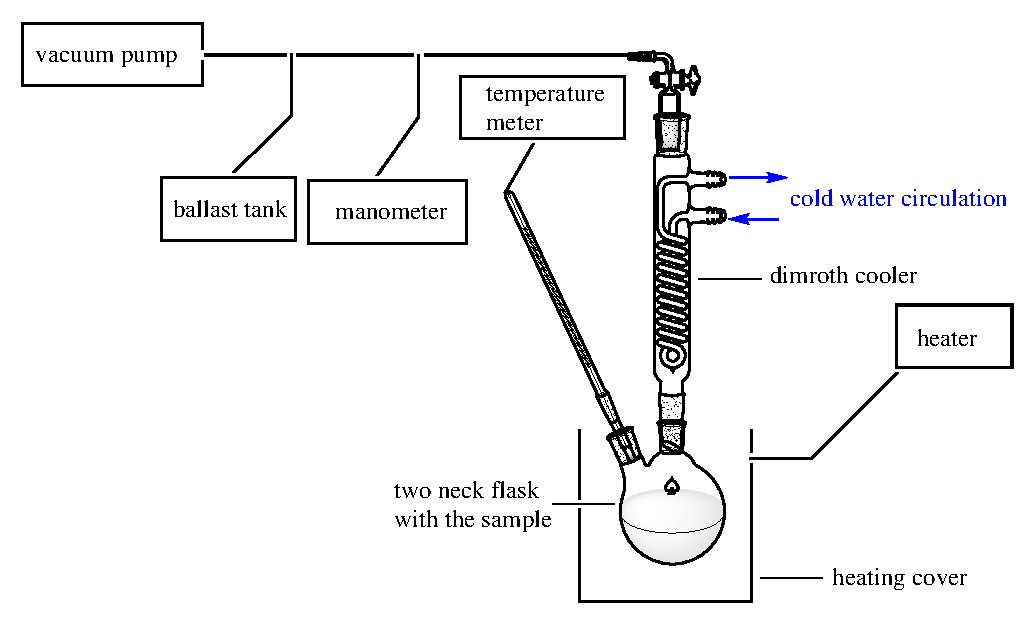
\includegraphics[scale = 0.8]{skizze1DDR.eps}
\caption{\label{fig:Skizze1}A schematic scheme of the used vapour pressure machinery. Details are described in the text.} 
\end{figure}

For the determination of the enthalpy of vaporisation out of transient evaporation cooling curves a TREVAC apparatus was used. The apparatus consists of four separate measuring cells, the schematic scheme of one measuring cell is depicted in Fig.\ref{fig:Skizze2}. Each measuring cell contains a highly sensitive temperature sensor (Semiconductor resistor NATIONAL LM 35). The inert \ce{N2} gas flows continuously over the temperature sensor and forces the evaporation rate of the analyzing liquid. The temperature in the block is kept at a constant 34.59 C$^{\circ}$ by circulating water (from a LAUDA Ecoline 103 thermostat). The \ce{N2} gas has also the temperature  34.59 C$^{\circ}$. The cells are connected to the software temperature logger (V21.7), which graphically displays the measured temperatures at a certain time interval. 

\\

5 $\mu$l of ethanol respectively n-hexane was injected into the measuring cell with a precision syringe (HAMILTON 801 RN). The measuring was stopped as soon as three meaningful peaks have been generated for each substance. The same procedure was done for the reference substance methanol. 

\begin{figure}[H]
\begin{minipage}[c]{0.55\textwidth}
\centering
 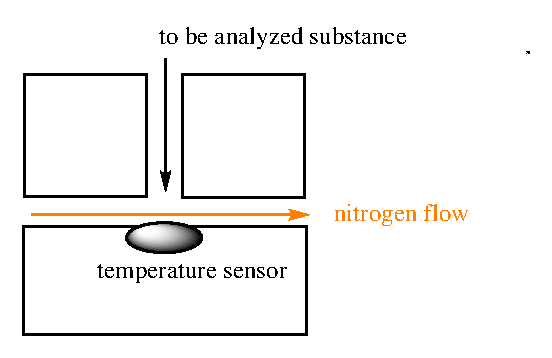
\includegraphics[scale=0.9] {skizze2DDR.eps}
 \end{minipage}\hfill
\begin{minipage}[c]{0.4\textwidth}
\caption{\label{fig:Skizze2} The schematic scheme of a measuring cell from a TREVAC apparatus. The cell contains a highly sensitive temperature sensor, which measures the transient cooling of the injected liquid. Through the flow of the inert gas the evaporation rate is accelerated. The to be analyzed liquid was injected by a precision syringe from HAMILTON.} 
\end{minipage}
\end{figure}


All measurements were plotted and the results calculated with Python (Version 3.8) as can be seen in the appendix. 

\newpage
\section*{Results and Discussion}
\subsection*{Density and refractive index determination}
The refractive index of ethanol and n-hexane was measured using a digital refractometer. The density was once determined by a density meter and once by weighing the substances. The buyoancy correction (Eq.\ref{eq:buoyancy}) was applied on the weighted mass and then the corrected mass was divided by the volume of the substance. All the results and the corresponding literature values are listed in Tab.\ref{tab:Teil1}. 

\begin{table}[H]
\centering
\begin{tabular}{c|c|c|c|c|c}
    substance &\thead{weighted\\ density $\rho$ [\si{\gram\per\cubic\centi\metre}]} &\thead{measured\\ density $\rho$ [\si{\gram\per\cubic\centi\metre}]} &\thead{reference \\ density $\rho$ [\si{\gram\per\cubic\centi\metre}]} & \thead{measured\\ refractive index $\eta$}& \thead{reference\\ refractive index $\eta$}\\
    \hline
    \thead{measuring\\ temperature [C$^{\circ}$]} & 25 & 20 & 25 & 19.8 & 20 \\
     \hline
    n-hexane & 0.6576 $\pm$ 0.0006 & 0.6594 $\pm$ 0.0006 & 0.659\cite{nhexane} & 1.37516 $\pm$ 0.00005 & 1.375\cite{nhexane}\\
    ethanol & 0.785 $\pm$ 0.002 & 0.7892 $\pm$ 0.0002 & 0.789\cite{ethanol} & 1.36125 $\pm$ 0.00004 & 1.3600\cite{ethanol}\\
\end{tabular}
\caption{\label{tab:Teil1} From the substances used for the vapour pressure and transient cooling experiments the density was determined by weighing and by using a density meter. The refractive index was measured by a digital refractometer. All the measured values correspond with the literature value, which verifies the identity of the used substances.}
\end{table}

The calculated density and refractive index values agree with the literature values. Therefore the identity and accurate purity of n-hexane and ethanol for the further experiments can be assumed. The density determination by using a density meter was more accurate than the weighing procedure. With the weighing method, the source of error is greater than with the density meter due to the manual pipetting and the measuring inaccuracy of the scale. 

\subsection*{Vapour pressure experiment}
The obtained experimental data of the boiling temperatures and the corresponding pressures were used to determine the enthalpy of vaporisation ($\Delta_{\textit{v}}$H), the entropy of vaporisation ($\Delta_{\textit{v}}$S), the normal boiling temperature (T$_{0}$) and the parameters A, B and C of the Antoine-Equation for the substances ethanol and n-hexane. The results are listed in Tab.\ref{tab:Teil2} with their corresponding literature values. $\Delta_{\textit{v}}$H and T$_{0}$ were extracted from fits of the Clausius-Clapeyron-Equation (Eq.\ref{eq:claus1}) using the experimental determined values. For both substances the experimental determined T$_{0}$ value match with the reference value. The reference values of the enthalpy of vaporisation do not lie within the 95\% confidence interval of the calculated enthalpies. The measured $\Delta_{\textit{v}}$H is for both substance higher than the reference value. For the Clausius-Clapeyron fit it was assumed that the normal pressure was 1013.25 mbar, which probably does not correspond to the exact laboratory conditions that existed. In addition the laboratory temperature was probably under 25 C$^{\circ}$, which was assumed as standard condition for the literature values\cite{reference}. The enthalpy of vaporisation is temperature dependent\cite{enthalpieT}. The lower the temperature, the higher the enthaply of vaporisation is, which would explain the higher measured enthaply of vaporisation. The parameters A, B and C obtained from a fit of the Antoine-Equation (Eq.\ref{eq:antoine}) deviate from the literature values. Different measuring conditions compared to the reference values could be the cause, similar to the deviation of the enthalpy of vaporisation. The entropy of vaporisation was calculated from the obtained data from the Clausius-Clapeyron fit, which can be seen in Fig.\ref{fig:DDR1} and the linearized Clausius-Clapeyron fit, depicted in Fig.\ref{fig:DDR2}. The $\Delta_{\textit{v}}$S values were determined using Eq.\ref{eq:entropy} resulting in too high values for both substances. The reason for the deviations are the too high $\Delta_{\textit{v}}$H values. 

\begin{table}[H]
\centering
\begin{tabular}{c|c|c|c|c|c|c}
    & $\Delta_{\textit{v}}$H [\si{\joule\per\mol}] & T_{0} [K] & A & B [C$^{\circ}$] & C [C$^{\circ}$] & $\Delta_{\textit{v}}$S [\si{\joule\per\mol\per\kelvin}]\\
    \hline
    n-hexane \\
    \hline
    measured & 30866.9 $\pm$ 236.4 & 342.30 $\pm$ 0.12 & 6.41 $\pm$ 0.18 & 861.07 $\pm$ 88.19 & 183.3 $\pm$ 10.4 & 91.3 $\pm$ 1.4\\
    literature & 28850\cite{meister} & 342.15\cite{nhexane}& 7.01045\cite{meister} & 1175.817\cite{meister} & 224.867\cite{meister} & 84\cite{meister}\\
    \hline
    ethanol \\
    \hline
    measured & 41216 $\pm$ 423 & 351.87 $\pm$ 0.13 & 7.69 & 1268.84 & 192 & 118.1 $\pm$ 1.3\\
    literature & 38560\cite{meister} & 351.39\cite{meister} & 8.23710\cite{meister} & 1592.865\cite{meister} & 226.184\cite{meister}& 110\cite{meister}\\
    
\end{tabular}
\caption{\label{tab:Teil2}The normal boiling temperature and the evaporation enthalpy from ethanol and n-hexane were determined using the Clausius-Clapeyron-Equation. The parameters A, B and C were calculated with the Antoine-Equation.}
\end{table}

In Fig.\ref{fig:DDR2} the correlation between the Clausius-Clapeyron-Equation, the Antoine-Equation and the experimental data of both solvents show a nearly perfect match. The agreement affirms the correctness of the models from Antoine and Clausius-Clapeyron. The normal pressure was assumed to be 1023.25 mbar, which yields directly to the normal boiling temperature T$_{0}$. In Fig.\ref{fig:DDR2} can be shown, that with increasing pressure the temperature rises exponentially. 

\begin{figure}[H]
    \centering
    % This file was created by tikzplotlib v0.9.8.
\begin{tikzpicture}

\definecolor{color0}{rgb}{0.75,0,0.75}

\begin{axis}[
legend cell align={left},
legend style={
  fill opacity=0.8,
  draw opacity=1,
  text opacity=1,
  at={(0.03,0.97)},
  anchor=north west,
  draw=white!80!black
},
width=\textwidth,
height=9cm,
tick align=outside,
tick pos=left,
x grid style={white!69.0196078431373!black},
xlabel={$\theta$ / C$^{\circ}$},
xmin=0.659523809523824, xmax=87.9611111111112,
xtick style={color=black},
y grid style={white!69.0196078431373!black},
ylabel={$\rho$/ \si{\milli\bar}},
ymin=0, ymax=1100,
ytick style={color=black}
]
\addplot [semithick, blue, mark=*, mark size=3, mark options={solid}, only marks]
table {%
30.7 101
38.4 150
43.4 200
47.7 241
51.2 291
54.6 351
57.3 399
59.9 451
62.2 500
64.4 550
66.5 599
68.3 648
70.1 699
71.3 749
73.2 799
74.4 851
75.9 898
77.3 948
75.9 899
74.4 849
72.9 799
71.3 749
69.7 699
68.1 649
66 599
64.2 549
62 499
59.7 449
57.2 400
54.4 349
51.2 301
};
\addlegendentry{ethanol data points}
\addplot [semithick, blue, mark=diamond*, mark size=3, mark options={solid}, only marks]
table {%
11.6 100
20.1 151
26.1 200
31 249
35.4 299
39.2 350
42.6 399
45.7 451
48.6 500
51.2 550
53.6 600
56 650
58.1 700
60.1 750
62.1 800
63.8 848
65.6 898
67.2 946
65.7 900
63.7 849
61.9 800
60 750
57.9 701
55.8 650
53.5 601
51 549
48.5 499
45.7 450
42.7 400
39.2 350
};
\addlegendentry{n-hexane data points}
\addplot [semithick, black, forget plot]
table {%
83.9928571428572 1606.4305711499
83.8907433881344 1601.55651171923
83.7886880091468 1596.69724063718
83.6866909558508 1591.85271303455
83.5847521782603 1587.02288417823
83.4828716264458 1582.20770947088
83.3810492505353 1577.40714445044
83.2792850007136 1572.62114478977
83.1775788272222 1567.84966629621
83.0759306803595 1563.0926649112
82.9743405104805 1558.35009670984
82.8728082679972 1553.62191790052
82.7713339033775 1548.90808482449
82.6699173671464 1544.20855395545
82.5685586098846 1539.52328189919
82.4672575822298 1534.85222539314
82.3660142348755 1530.19534130601
82.2648285185713 1525.55258663737
82.1637003841229 1520.92391851724
82.0626297823923 1516.30929420573
81.9616166642969 1511.70867109262
81.8606609808103 1507.12200669697
81.7597626829615 1502.54925866675
81.6589217218355 1497.99038477841
81.5581380485727 1493.44534293651
81.4574116143689 1488.91409117334
81.3567423704755 1484.39658764852
81.2561302681992 1479.89279064862
81.155575258902 1475.40265858678
81.0550772940009 1470.92615000231
80.9546363249681 1466.46322356029
80.854252303331 1462.01383805127
80.7539251806717 1457.57795239079
80.6536549086273 1453.15552561905
80.5534414388897 1448.74651690054
80.4532847232055 1444.35088552364
80.3531847133758 1439.96859090027
80.2531413612566 1435.59959256545
80.153154618758 1431.24385017703
80.0532244378447 1426.90132351523
79.9533507705358 1422.57197248232
79.8535335689047 1418.2557571022
79.7537727850784 1413.95263752009
79.6540683712389 1409.66257400213
79.5544202796216 1405.38552693501
79.4548284625159 1401.1214568256
79.3552928722654 1396.8703243006
79.2558134612671 1392.6320901062
79.1563901819721 1388.40671510765
79.0570229868848 1384.19416028897
78.9577118285634 1379.99438675253
78.8584566596195 1375.80735571875
78.7592574327181 1371.63302852568
78.6601141005776 1367.47136662869
78.5610266159696 1363.32233160011
78.461994931719 1359.18588512884
78.3630190007038 1355.06198902002
78.2640987758548 1350.9506051947
78.1652342101561 1346.85169568944
78.0664252566447 1342.765222656
77.96767186841 1338.69114836098
77.8689739985945 1334.62943518544
77.7703316003934 1330.58004562461
77.6717446270544 1326.54294228749
77.5732130318776 1322.51808789654
77.4747367682156 1318.50544528732
77.3763157894737 1314.50497740816
77.2779500491091 1310.51664731978
77.1796395006313 1306.54041819502
77.081384097602 1302.57625331841
76.9831837936352 1298.62411608592
76.8850385423967 1294.68397000455
76.7869482976041 1290.75577869204
76.688913013027 1286.83950587652
76.5909326424871 1282.93511539614
76.4930071398572 1279.04257119882
76.3951364590623 1275.16183734182
76.2973205540786 1271.29287799147
76.1995593789341 1267.43565742284
76.101852887708 1263.59014001936
76.004201034531 1259.75629027256
75.9066037735849 1255.93407278167
75.809061059103 1252.12345225335
75.7115728453695 1248.32439350134
75.6141390867198 1244.53686144614
75.5167597375402 1240.76082111468
75.419434752268 1236.99623764001
75.3221640853914 1233.24307626095
75.2249476914494 1229.50130232182
75.1277855250314 1225.77088127205
75.030677540778 1222.05177866594
74.9336236933798 1218.34396016226
74.8366239375784 1214.64739152402
74.7396782281655 1210.96203861807
74.6427865199833 1207.28786741483
74.5459487679243 1203.624843988
74.4491649269311 1199.97293451417
74.3524349519967 1196.33210527258
74.2557587981639 1192.70232264479
74.1591364205257 1189.08355311433
74.062567774225 1185.47576326645
73.9660528144545 1181.87891978778
73.8695914964569 1178.29298946601
73.7731837755244 1174.71793918961
73.6768296069991 1171.15373594753
73.5805289462724 1167.60034682883
73.4842817487856 1164.05773902248
73.3880879700292 1160.52587981697
73.2919475655431 1157.00473660005
73.1958604909167 1153.49427685841
73.0998267017885 1149.9944681774
73.0038461538462 1146.50527824072
72.9079188028267 1143.0266748301
72.8120446045158 1139.55862582504
72.7162235147487 1136.10109920251
72.6204554894089 1132.65406303661
72.5247404844291 1129.21748549832
72.4290784557908 1125.7913348552
72.3334693595241 1122.37557947108
72.237913151708 1118.97018780578
72.1424097884695 1115.57512841482
72.0469592259848 1112.19036994911
71.9515614204781 1108.81588115469
71.8562163282222 1105.45163087243
71.7609239055379 1102.09758803774
71.6656841087947 1098.75372168025
71.57049689441 1095.42000092362
71.4753622188492 1092.09639498513
71.380280038626 1088.78287317548
71.285250310302 1085.47940489851
71.1902729904867 1082.18595965085
71.0953480358374 1078.90250702171
71.0004754030591 1075.62901669255
70.9056550489048 1072.36545843683
70.8108869301749 1069.11180211972
70.7161710037175 1065.86801769782
70.6215072264281 1062.63407521888
70.5268955552498 1059.40994482153
70.4323359471729 1056.19559673501
70.3378283592353 1052.99100127888
70.2433727485219 1049.79612886275
70.148969072165 1046.61094998601
70.0546172873437 1043.43543523758
69.9603173512846 1040.26955529558
69.8660692212608 1037.11328092712
69.7718728545929 1033.966582988
69.6777282086479 1030.82943242244
69.5836352408399 1027.70180026283
69.4895939086294 1024.58365762944
69.3956041695241 1021.47497573016
69.3016659810778 1018.37572586025
69.207779300891 1015.28587940206
69.113944086611 1012.20540782477
69.020160295931 1009.1342826841
68.9264278865909 1006.07247562212
68.8327468163769 1003.01995836691
68.7391170431212 999.976702732313
68.6455385247024 996.942680617734
68.552011219045 993.91786400781
68.4585350841199 990.902224972188
68.3651100779434 987.895735665249
68.2717361585783 984.898368325873
68.1784132841329 981.910095277164
68.0851414127613 978.930888926195
67.9919205026636 975.960721763769
67.8987505120853 972.999566364149
67.8056313993175 970.047395384809
67.7125631226969 967.10418156618
67.6195456406058 964.16989773141
67.5265789114719 961.244516786099
67.4336628937679 958.328011718052
67.3407975460123 955.420355597038
67.2479828267685 952.521521574524
67.1552186946451 949.631482883451
67.0625051082959 946.750212837962
66.9698420264198 943.877684833176
66.8772294077604 941.013872344928
66.7846672111066 938.158748929533
66.6921553952919 935.31228822354
66.5996939191947 932.47446394348
66.5072827417381 929.645249885638
66.4149218218899 926.824619925801
66.3226111186626 924.012548019017
66.230350591113 921.209008199363
66.1381401983426 918.413974579689
66.0459798994975 915.627421351401
65.9538696537679 912.8493227842
65.8618094203882 910.079653225859
65.7697991586376 907.318387101989
65.6778388278389 904.565498915785
65.5859283873593 901.820963247807
65.4940677966102 899.08475475574
65.4022570150468 896.356848174161
65.3104960021683 893.637218314302
65.218784717518 890.925840063821
65.1271231206827 888.222688386568
65.0355111712932 885.527738322361
64.943948829024 882.840964986741
64.8524360535932 880.162343570755
64.7609728047626 877.491849340721
64.6695590423374 874.829457638008
64.5781947261664 872.175143878791
64.4868798161417 869.52888355384
64.3956142721989 866.890652228291
64.304398054317 864.260425541413
64.2132311225179 861.638179206392
64.122113436867 859.023889010097
64.0310449574727 856.417530812862
63.9400256444865 853.819080548271
63.8490554581028 851.228514222921
63.7581343585593 848.64580791621
63.6672623061362 846.070937780107
63.5764392611568 843.50388003895
63.4856651839871 840.944610989204
63.3949400350357 838.393106999254
63.3042637747541 835.84934450919
63.2136363636364 833.313300030587
63.123057762219 830.784950146279
63.0325279310809 828.264271510152
62.9420468308438 825.751240846924
62.8516144221714 823.245834951943
62.76123066577 820.748030690949
62.6708955223881 818.257804999881
62.5806089528162 815.775134884654
62.4903709178874 813.299997420952
62.4001813784765 810.832369754007
62.3100402955004 808.372229098403
62.2199476299181 805.919552737848
62.1299033427306 803.474318024982
62.0399073949806 801.036502381154
61.9499597477526 798.606083296222
61.860060362173 796.183038328337
61.77020919941 793.767345103743
61.680406220673 791.358981316573
61.5906513872135 788.957924728629
61.5009446603243 786.564153169195
61.4112860013396 784.177644534813
61.3216753716353 781.798376789099
61.2321127326282 779.426327962521
61.142598045777 777.061476152214
61.0531312725813 774.703799521757
60.963712374582 772.353276300991
60.874341313361 770.009884785808
60.7850180505415 767.673603337946
60.6957425477877 765.34441038481
60.6065147668048 763.022284419245
60.5173346693387 760.707203999351
60.4282022171765 758.399147748293
60.3391173721458 756.09809435409
60.2500800961154 753.804022569424
60.1610903509942 751.516911211443
60.0721480987325 749.23673916157
59.9832533013206 746.963485365298
59.8944059207895 744.697128832003
59.8056059192108 742.437648634746
59.7168532586965 740.185023910092
59.6281479013991 737.939233857895
59.5394898095112 735.70025774113
59.4508789452657 733.468074885681
59.362315270936 731.242664680163
59.2737987488354 729.024006575727
59.1853293413174 726.812080085875
59.0969070107756 724.606864786261
59.0085317196436 722.40834031451
58.9202034303949 720.216486370031
58.8319221055431 718.031282713827
58.7436877076412 715.8527091683
58.6555001992826 713.680745617087
58.5673595431001 711.515372004848
58.4792657017661 709.356568337096
58.3912186379928 707.204314680008
58.3032183145322 705.058591160251
58.2152646941755 702.919377964773
58.1273577397533 700.786655340653
58.0394974141361 698.66040359489
57.9516836802334 696.540603094244
57.8639165009941 694.427234265036
57.7761958394065 692.320277592975
57.6885216584978 690.219713622986
57.6008939213349 688.125522959014
57.5133125910235 686.03768626386
57.4257776307082 683.956184258992
57.3382890035729 681.88099772437
57.2508466728403 679.812107498275
57.1634506017723 677.749494477119
57.0761007536692 675.693139615281
56.9887970918705 673.643023924925
56.9015395797542 671.599128475825
56.8143281807373 669.561434395194
56.7271628582751 667.529922867502
56.6400435758616 665.504575134311
56.5529702970297 663.485372494095
56.4659429853505 661.472296302073
56.3789616044334 659.465327970033
56.2920261179264 657.46444896616
56.2051364895161 655.469640814869
56.1182926829269 653.480885096628
56.0314946619217 651.498163447791
55.9447423903018 649.521457560437
55.8580358319062 647.550749182185
55.7713749506124 645.586020116035
55.6847597103358 643.627252220201
55.5981900750297 641.674427407937
55.5116660086854 639.727527647377
55.4251874753322 637.786534961363
55.3387544390372 635.851431427285
55.2523668639054 633.922199176907
55.1660247140792 631.998820396212
55.0797279537391 630.081277325229
54.9934765471029 628.169552257871
54.9072704584264 626.263627541777
54.8211096520026 624.363485578142
54.7349940921623 622.469108821561
54.6489237432734 620.580479779858
54.5628985697415 618.697581013933
54.4769185360095 616.820395137598
54.3909836065574 614.948904817418
54.3050937459027 613.083092772541
54.2192489186001 611.222941774561
54.1334490892413 609.36843464733
54.0476942224552 607.519554266822
53.9619842829077 605.676283560966
53.8763192353018 603.838605509487
53.7906990443776 602.006503143758
53.7051236749117 600.179959546623
53.6195930917179 598.358957852269
53.5341072596469 596.543481246044
53.4486661435857 594.73351296432
53.3632697084587 592.92903629433
53.2779179192262 591.13003457401
53.1926107408859 589.336491191861
53.1073481384717 587.548389586776
53.0221300770537 585.765713247897
52.9369565217391 583.988445714463
52.8518274376714 582.216570575657
52.76674279003 580.450071470454
52.6817025440313 578.688932087468
52.5967066649276 576.933136164805
52.5117551180076 575.182667489911
52.426847868596 573.43750989942
52.341984882054 571.697647279011
52.2571661237785 569.963063563252
52.1723915592028 568.233742735459
52.0876611537961 566.509668827537
52.0029748730635 564.79082591985
51.9183326825459 563.077198141052
51.8337345478205 561.368769667962
51.7491804344999 559.665524725402
51.6646703082325 557.967447586059
51.5802041347029 556.274522570341
51.4957818796308 554.586734046225
51.411403508772 552.90406642912
51.3270689879174 551.226504181715
51.2427782828939 549.55403181385
51.1585313595637 547.886633882354
51.0743281838245 546.22429499092
50.9901687216093 544.566999789946
50.9060529388867 542.914732976411
50.8219808016604 541.267479293721
50.7379522759695 539.62522353157
50.653967327888 537.987950525803
50.5700259235256 536.355645158276
50.4861280290269 534.728292356713
50.4022736105713 533.105877094568
50.3184626343738 531.488384390891
50.234695066684 529.875799310181
50.1509708737864 528.268106962254
50.0672900220008 526.665292502107
49.9836524776815 525.067341129774
49.9000582072177 523.474238090195
49.8165071770335 521.885968673079
49.7329993535876 520.302518212767
49.6495347033734 518.723872088097
49.566113192919 517.150015722269
49.482734788787 515.580934582709
49.3993994575746 514.01661418094
49.3161071659135 512.457040072438
49.2328578804699 510.902197856512
49.1496515679443 509.352073176157
49.0664881950717 507.806651717938
48.9833677286212 506.265919211837
48.9002901353965 504.729861431142
48.8172553822354 503.1984641923
48.7342634360098 501.671713354795
48.6513142636258 500.149594821015
48.5684078320238 498.632094536122
48.4855441081777 497.119198487915
48.4027230590962 495.610892706718
48.3199446518213 494.107163265232
48.2372088534294 492.607996278419
48.1545156310305 491.113377903367
48.0718649517685 489.623294339168
47.9892567828211 488.137731826782
47.9066910913999 486.65667664892
47.8241678447501 485.180115129912
47.7416870101504 483.708033635576
47.6592485549133 482.240418573105
47.576852446385 480.777256390931
47.4944986519451 479.318533578598
47.4121871390066 477.864236666649
47.3299178750161 476.41435222649
47.2476908274535 474.968866870273
47.1655059638323 473.527767250768
47.083363251699 472.091040061244
47.0012626586336 470.658672035342
46.9192041522492 469.230649946955
46.8371877001922 467.806960610107
46.7552132701422 466.387590878825
46.6732808298117 464.972527647026
46.5913903469466 463.561757848393
46.5095417893255 462.155268456248
46.4277351247601 460.753046483443
46.3459703210951 459.355078982229
46.264247346208 457.961353044146
46.1825661680093 456.571855799899
46.100926754442 455.186574419235
46.0193290734824 453.805496110838
45.9377730931392 452.428608122192
45.8562587814536 451.05589773948
45.7747861064998 449.687352287458
45.6933550363846 448.322959129339
45.611965539247 446.962705666678
45.530617583259 445.606579339255
45.4493111366246 444.254567624959
45.3680461675807 442.906658039672
45.2868226443963 441.562838137153
45.2056405353729 440.223095508926
45.1244998088442 438.887417784162
45.0434004331762 437.555792629566
44.9623423767673 436.228207749266
44.8813256080479 434.904650884694
44.8003500954806 433.585109814474
44.7194158075602 432.269572354318
44.6385227128134 430.958026356896
44.557670779799 429.650459711744
44.476859977108 428.346860345137
44.396090273363 427.047216219981
44.3153616372188 425.751515335711
44.2346740373619 424.459745728164
44.1540274425105 423.171895469483
44.073421821415 421.887952668002
43.9928571428572 420.607905468132
43.9123333756507 419.331742050254
43.8318504886407 418.059450630614
43.7514084507043 416.791019461212
43.6710072307498 415.526436829689
43.5906467977172 414.265691059223
43.5103271205782 413.008770508424
43.4300481683357 411.755663571218
43.3498099100241 410.50635867675
43.2696123147093 409.260844289268
43.1894553514883 408.019108908021
43.1093389894897 406.781141067155
43.0292631978732 405.546929335603
42.9492279458297 404.31646231698
42.8692332025813 403.089728649479
42.7892789373814 401.866717005767
42.7093651195144 400.647416092879
42.6294917182956 399.431814652112
42.5496587030717 398.219901458925
42.4698660432201 397.011665322832
42.3901137081491 395.807095087301
42.3104016672983 394.606179629652
42.2307298901376 393.408907860944
42.1510983461685 392.215268725891
42.0715070049224 391.025251202745
41.9919558359622 389.838844303199
41.912444808881 388.656037072283
41.8329738933031 387.476818588274
41.7535430588829 386.301177962575
41.6741522753057 385.129104339637
41.5948015122873 383.960586896837
41.5154907395741 382.795614844401
41.436219926943 381.63417742528
41.356989044201 380.476263915072
41.277798061186 379.321863621909
41.1986469477659 378.170965886364
41.1195356738392 377.023560081353
41.0404642093346 375.879635612035
40.9614325242108 374.739181915713
40.8824405884572 373.60218846174
40.8034883720931 372.468644751421
40.7245758451678 371.338540317912
40.6457029777611 370.21186472613
40.5668697399825 369.088607572648
40.4880761019717 367.96875848561
40.4093220338984 366.852307124625
40.3306075059621 365.739243180675
40.2519324883925 364.629556376025
40.1732969514491 363.523236464121
40.0947008654208 362.420273229494
40.016144200627 361.320656487679
39.9376269274164 360.224376085105
39.8591490161675 359.131421899005
39.7807104372886 358.041783837334
39.7023111612176 356.955451838661
39.6239511584221 355.872415872084
39.545630399399 354.792665937136
39.4673488546752 353.716192063693
39.3891064948067 352.642984311878
39.3109032903791 351.573032771978
39.2327392120076 350.506327564342
39.1546142303364 349.442858839296
39.0765283160395 348.382616777052
38.9984814398201 347.325591587618
38.9204735724104 346.2717735107
38.8425046845721 345.221152815622
38.7645747470963 344.173719801232
38.6866837308029 343.129464795809
38.6088316065411 342.088378156982
38.5310183451891 341.050450271628
38.4532439176544 340.015671555801
38.3755082948734 338.984032454625
38.2978114478115 337.95552344222
38.2201533474629 336.930135021603
38.1425339648511 335.907857724611
38.0649532710281 334.888682111806
37.9874112370749 333.872598772392
37.9099078341014 332.859598324121
37.8324430332462 331.849671413219
37.7550168056766 330.842808714286
37.6776291225887 329.839000930219
37.6002799552072 328.838238792122
37.5229692747855 327.840513059225
37.4456970526055 326.84581451879
37.3684632599777 325.854133986035
37.2912678682412 324.865462304046
37.2141108487635 323.879790343689
37.1369921729408 322.897109003531
37.0599118121973 321.917409209753
36.9828697379859 320.940681916065
36.9058659217877 319.966918103627
36.8289003351123 318.996108780963
36.7519729494975 318.028244983875
36.6750837365091 317.063317775365
36.5982326677416 316.101318245553
36.5214197148172 315.142237511588
36.4446448493865 314.186066717573
36.3679080431281 313.23279703448
36.2912092677487 312.28241966007
36.2145484949833 311.33492581881
36.1379256965944 310.390306761791
36.0613408443729 309.448553766653
35.9847939101374 308.509658137498
35.9082848657345 307.573611204812
35.8318136830385 306.640404325385
35.7553803339518 305.710028882232
35.6789847904044 304.782476284514
35.6026270243541 303.857737967455
35.5263070077864 302.935805392266
35.4500247127147 302.016670046066
35.3737801111798 301.100323441803
35.2975731752501 300.186757118174
35.2214038770219 299.275962639551
35.1452721886187 298.367931595898
35.0691780821918 297.462655602698
34.9931215299198 296.560126300872
34.9171025040089 295.660335356702
34.8411209766926 294.763274461758
34.7651769202318 293.868935332818
34.6892703069149 292.977309711789
34.6134011090573 292.088389365638
34.5375692990021 291.202166086311
34.4617748491194 290.318631690654
34.3860177318065 289.437778020347
34.3102979194879 288.559596941818
34.2346153846154 287.684080346179
34.1589700996678 286.811220149138
34.083362037151 285.941008290939
34.0077911695979 285.073436736272
33.9322574695685 284.208497474213
33.8567609096497 283.346182518144
33.7813014624555 282.486483905673
33.7058791006266 281.629393698573
33.6304937968309 280.7749039827
33.5551455237628 279.923006867924
33.4798342541437 279.073694488049
33.4045599607218 278.226959000752
33.329322616272 277.3827925875
33.2541221935959 276.541187453486
33.1789586655219 275.70213582755
33.103832004905 274.865629962111
33.0287421846267 274.031662133097
32.9536891775953 273.200224639868
32.8786729567456 272.371309805153
32.8036934950386 271.544909974969
32.7287507654624 270.721017518561
32.653844741031 269.899624828323
32.5789753947852 269.080724319733
32.5041426997919 268.26430843128
32.4293466291448 267.450369624397
32.3545871559633 266.638900383388
32.2798642533937 265.829893215361
32.2051778946081 265.023340650159
32.1305280528053 264.219235240288
32.0559147012099 263.417569560853
31.9813378130727 262.618336209482
31.906797361671 261.82152780627
31.8322933203078 261.027136993698
31.7578256623123 260.235156436571
31.6833943610399 259.44557882195
31.6089993898719 258.658396859086
31.5346407222155 257.873603279348
31.4603183315039 257.09119083616
31.3860321911963 256.311152304934
31.3117822747776 255.533480482998
31.2375685557587 254.75816818954
31.1633910076764 253.985208265528
31.0892496040931 253.214593573659
31.015144318597 252.446316998277
30.9410751248022 251.680371445322
30.8670419963482 250.916749842254
30.7930449069004 250.155445137995
30.7190838301497 249.396450302858
30.6451587398127 248.639758328486
30.5712696096315 247.885362227786
30.4974164133739 247.133255034864
30.4235991248329 246.383429804961
30.3498177178272 245.635879614391
30.276072166201 244.890597560471
30.2023624438237 244.147576761465
30.1286885245902 243.406810356517
30.0550503824208 242.668291505585
29.9814479912611 241.932013389382
29.9078813250819 241.19796920931
29.8343503578794 240.4661521874
29.760855063675 239.736555566248
29.6873954165151 239.009172608952
29.6139713904716 238.28399659905
29.5405829596413 237.561020840458
29.4672300981462 236.840238657411
29.3939127801333 236.121643394396
29.3206309797748 235.405228416095
29.2473846712678 234.690987107322
29.1741738288343 233.978912872963
29.1009984267216 233.26899913791
29.0278584392015 232.56123934701
28.954753840571 231.855626964997
28.8816846051518 231.152155476432
28.8086507072906 230.450818385647
28.7356521213587 229.751609216679
28.6626888217523 229.054521513216
28.5897607828924 228.359548838536
28.5168679792246 227.666684775446
28.4440103852192 226.97592292622
28.3711879753713 226.287256912549
28.2984007242004 225.600680375471
28.2256486062508 224.916186975322
28.1529315960912 224.233770391671
28.080249668315 223.553424323262
28.0076027975401 222.875142487962
27.9349909584087 222.198918622696
27.8624141255876 221.52474648339
27.789872273768 220.852619844919
27.7173653776654 220.182532501042
27.6448934120198 219.514478264352
27.5724563515955 218.848450966211
27.500054171181 218.184444456701
27.4276868455892 217.522452604561
27.3553543496571 216.862469297133
27.2830566582462 216.204488440308
27.2107937462418 215.548503958463
27.1385655885536 214.894509794411
27.0663721601155 214.242499909345
26.9942134358851 213.592468282776
26.9220893908447 212.944408912486
26.85 212.298315814466
26.7779452383812 211.654183022862
26.7059250810422 211.012004589925
26.6339395030609 210.371774585948
26.5619884795393 209.733487099217
26.4900719856029 209.097136235954
26.4181899964016 208.462716120263
26.3463424871088 207.830220894079
26.2745294329218 207.199644717107
26.2027508090615 206.570981766773
26.1310065907729 205.94422623817
26.0592967533246 205.319372344006
25.9876212720087 204.696414314542
25.9159801221411 204.075346397552
25.8443732790614 203.456162858256
25.7728007181329 202.838857979281
25.7012624147422 202.223426060593
25.6297583442995 201.60986141946
25.558288482239 200.998158390387
25.4868528040178 200.388311325071
25.4154512851166 199.780314592344
25.3440839010399 199.174162578129
25.2727506273151 198.569849685374
25.2014514394936 197.967370334018
25.1301863131495 197.366718960923
25.0589552238806 196.767890019835
24.9877581473081 196.170877981327
24.9165950590763 195.575677332747
24.8454659348527 194.982282578169
24.774370750328 194.390688238344
24.7033094812165 193.800888850647
24.6322821032551 193.212878969025
24.5612885922041 192.626653163952
24.490328923847 192.042206022374
24.4194030739903 191.45953214766
24.3485110184634 190.878626159555
24.277652733119 190.299482694126
24.2068281938326 189.722096403716
24.1360373765028 189.146461956893
24.0652802570511 188.572574038401
23.9945568114218 188.000427349111
23.9238670155823 187.430016605972
23.8532108455227 186.861336541962
23.782588277256 186.29438190604
23.711999286818 185.729147463097
23.6414438502674 185.165627993908
23.5709219436854 184.603818295084
23.5004335431762 184.043713179022
23.4299786248665 183.485307473861
23.3595571649057 182.928596023429
23.2891691394659 182.373573687201
23.218814524742 181.820235340248
23.148493296951 181.268575873189
23.0782054323331 180.718590192148
23.0079509071505 180.170273218702
22.9377296976883 179.623619889838
22.8675417802537 179.078625157904
22.7973871311767 178.535283990562
22.7272657268097 177.993591370743
22.6571775435272 177.453542296603
22.5871225577265 176.915131781471
22.517100745827 176.378354853807
22.4471120842704 175.843206557154
22.3771565495208 175.309681950096
22.3072341180646 174.777776106207
22.2373447664104 174.247484114009
22.1674884710891 173.718801076927
22.0976652086536 173.191722113242
22.027874955679 172.666242356046
21.9581176887629 172.142356953198
21.8883933845245 171.620061067279
21.8187020196056 171.099349875548
21.7490435706695 170.580218569894
21.6794180144021 170.062662356798
21.609825327511 169.546676457282
21.5402654867257 169.032256106868
21.4707384687979 168.519396555536
21.4012442505013 168.008093067678
21.3317828086311 167.49834092205
21.2623541200048 166.990135411737
21.1929581614614 166.483471844104
21.1235949098622 165.978345540755
21.0542643420898 165.474751837486
20.9849664350489 164.972686084246
20.9157011656658 164.472143645094
20.8464685108888 163.973119898152
20.7772684476874 163.47561023557
20.7081009530533 162.979610063471
20.6389660039995 162.485114801925
20.5698635775609 161.992119884892
20.5007936507937 161.500620760187
20.4317562007759 161.010612889438
20.3627512046069 160.522091748041
20.2937786394078 160.035052825123
20.2248384823212 159.549491623495
20.1559307105109 159.065403659612
20.0870553011624 158.582784463536
20.0182122314826 158.101629578888
19.9494014786997 157.621934562812
19.8806230200634 157.14369498593
19.8118768328446 156.666906432305
19.7431628943357 156.191564499399
19.6744811818502 155.717664798029
19.605831672723 155.245202952331
19.5372143443104 154.774174599718
19.4686291739895 154.304575390838
19.400076139159 153.836400989537
19.3315552172386 153.369647072817
19.2630663856692 152.904309330795
19.1946096219127 152.440383466666
19.1261849034523 151.977865196661
19.0577922077922 151.516750250009
18.9894315124576 151.057034368898
18.9211027949948 150.598713308432
18.8528060329709 150.141782836595
18.7845412039744 149.686238734214
18.7163082856142 149.232076794914
18.6481072555205 148.779292825084
18.5799380913445 148.327882643838
18.5118007707579 147.877842082972
18.4436952714536 147.429166986932
18.3756215711451 146.981853212772
18.3075796475669 146.535896630112
18.239569478474 146.09129312111
18.1715910416424 145.648038580413
18.1036443148689 145.206128915127
18.0357292759707 144.765560044776
17.9678459027859 144.326327901262
17.8999941731733 143.888428428832
17.8321740650123 143.451857584039
17.7643855562027 143.016611335704
17.6966286246653 142.582685664876
17.6289032483409 142.150076564803
17.5612094051915 141.718780040886
17.4935470731992 141.288792110647
17.4259162303665 140.860108803691
17.3583168547168 140.432726161671
17.2907489242936 140.006640238248
17.2232124171608 139.581847099058
17.155707311403 139.158342821673
17.088233585125 138.736123495567
17.0207912164518 138.315185222079
16.9533801835289 137.895524114376
16.8860004645222 137.477136297418
16.8186520376176 137.060017907924
16.7513348810215 136.644165094333
16.6840489729605 136.229574016769
16.6167942916812 135.816240847009
16.5495708154507 135.404161768444
16.482378522556 134.993332976044
16.4152173913044 134.583750676326
16.3480874000232 134.175411087314
16.2809885270599 133.768310438509
16.2139207507821 133.362444970853
16.1468840495772 132.95781093669
16.079878401853 132.554404599736
16.0129037860369 132.152222235046
15.9459601805765 131.751260128972
15.8790475639394 131.351514579138
15.812165914613 130.952981894399
15.7453152111047 130.555658394809
15.6784954319418 130.15954041159
15.6117065556712 129.76462428709
15.5449485608601 129.370906374762
15.478221426095 128.978383039117
15.4115251299827 128.587050655698
15.3448596511494 128.196905611047
15.2782249682411 127.807944302666
15.2116210599238 127.420163138992
15.1450479048829 127.033558539354
15.0785054818235 126.648126933949
15.0119937694705 126.263864763802
14.9455127465683 125.88076848074
14.879062391881 125.498834547352
14.8126426841924 125.118059436962
14.7462536023055 124.738439633593
14.6798951250432 124.359971631936
14.6135672312479 123.982651937319
14.5472698997812 123.60647706567
14.4810031095244 123.231443543491
14.4147668393783 122.857547907822
14.3485610682629 122.484786706209
14.282385775118 122.113156496675
14.2162409389023 121.742653847683
14.1501265385943 121.373275338112
14.0840425531915 121.005017557217
14.017988961711 120.637877104604
13.9519657431889 120.271850590195
13.8859728766809 119.906934634199
13.8200103412616 119.543125867077
13.7540781160253 119.180420929516
13.688176180085 118.818816472395
13.6223045125732 118.458309156755
13.5564630926415 118.098895653765
13.4906518994606 117.740572644697
13.4248709122203 117.383336820891
13.3591201101297 117.027184883726
13.2933994724166 116.67211354459
13.2277089783282 116.318119524848
13.1620486071306 115.965199555812
13.0964183381089 115.613350378714
13.0308181505673 115.262568744671
12.9652480238286 114.912851414658
12.8997079372352 114.564195159479
12.8341978701478 114.216596759733
12.7687178019463 113.87005300579
12.7032677120293 113.524560697755
12.6378475798147 113.180116645445
12.5724573847386 112.836717668354
12.5070971062565 112.494360595627
12.4417667238422 112.15304226603
12.3764662169887 111.81275952792
12.3111955652075 111.473509239215
12.2459547480288 111.135288267369
12.1807437450017 110.798093489339
12.1155625356939 110.461921791557
12.0504110996917 110.126770069903
11.9852894166001 109.792635229675
11.9201974660427 109.45951418556
11.8551352276618 109.127403861607
11.7901026811181 108.796301191197
11.725099806091 108.466203117015
11.6601265822785 108.137106591024
11.5951829893969 107.809008574433
11.5302690071812 107.481906037672
11.4653846153847 107.155795960363
11.4005297937792 106.830675331291
11.3357045221552 106.50654114838
11.2709087803212 106.183390418659
11.2061425481043 105.861220158242
11.1414058053501 105.540027392291
11.0766985319222 105.219809155
11.0120207077028 104.900562489557
10.9473723125924 104.582284448123
10.8827533265098 104.264972091803
10.8181637293918 103.94862249062
10.7536035011937 103.633232723483
10.6890726218888 103.318799878168
10.6245710714692 103.005321051286
10.5600988299444 102.692793348256
10.4956558773425 102.381213883279
10.4312421937096 102.070579779314
10.36685775911 101.760888168047
10.3025025536262 101.452136189869
10.2381765573585 101.144320993845
10.1738797504254 100.83743973769
10.1096121129636 100.531489587746
10.0453736251276 100.226467718949
9.98116426708992 99.9223713148086
9.91698401904119 99.6191975673783
9.85283286118982 99.3169436772325
9.78871077376238 99.0156068534387
9.72461773700309 98.7151843135328
9.66055373117428 98.4156732834918
9.59651873655611 98.1170709977113
9.53251273344654 97.8193746989761
9.46853570216143 97.5225816384379
9.40458762303433 97.2266890755878
9.34066847641674 96.9316942782324
9.27677824267784 96.6375945224679
9.21291690220465 96.3443870926551
9.14908443540185 96.0520692813941
9.08528082269186 95.7606383894999
9.02150604451481 95.4700917259766
8.95776008132839 95.1804266079933
8.89404291360819 94.8916403608591
8.83035452184714 94.6037303179982
8.76669488655608 94.3166938209255
8.70306398826324 94.0305282192225
8.63946180751441 93.7452308705109
8.57588832487312 93.4607991404313
8.5123435209203 93.1772304026164
8.44882737625437 92.8945220386672
8.3853398714914 92.6126714381298
8.32188098726476 92.3316759984701
8.25845070422537 92.0515331250511
8.19504900304162 91.7722402311078
8.13167586439914 91.4937947377228
8.06833126900125 91.2161940738046
8.00501519756841 90.9394356760628
7.9417276308385 90.6635169889828
7.87846854956683 90.388435464805
7.81523793452584 90.1141885634989
7.75203576650551 89.8407737527419
7.6888620263129 89.5681885078941
7.62571669477239 89.2964303119747
7.56259975272565 89.0254966556411
7.49951118103161 88.7553850371639
7.43645096056622 88.4860929624036
7.37341907222287 88.2176179447888
7.3104154969119 87.9499575052919
7.24744021556086 87.6831091724077
7.18449320911441 87.4170704821288
7.12157445853444 87.1518389779251
7.05868394479978 86.8874122107187
6.99582164890637 86.6237877388629
6.93298755186726 86.3609631281193
6.87018163471242 86.0989359516349
6.80740387848897 85.8377037899204
6.74465426426093 85.5772642308271
6.68193277310928 85.3176148695248
6.61923938613199 85.0587533084806
6.55657408444398 84.8006771574349
6.49393684917709 84.5433840333812
6.43132766147994 84.286871560543
6.36874650251821 84.0311373703516
6.30619335347433 83.7761791014255
6.24366819554763 83.521994399548
6.1811710099542 83.2685809176446
6.1187017779269 83.0159363157617
6.05626048071554 82.7640582610468
5.9938470995865 82.5129444277244
5.93146161582303 82.2625924970756
5.8691040107251 82.0130001574174
5.80677426560931 81.7641651040799
5.74447236180907 81.5160850393865
5.68219828067441 81.2687576726313
5.61995200357188 81.0221807200589
5.55773351188486 80.7763519048428
5.49554278701333 80.5312689570658
5.43337981037371 80.2869296136957
5.37124456339916 80.0433316185684
5.30913702753935 79.8004727223645
5.24705718426043 79.558350682589
5.18500501504519 79.3169632635513
5.12298050139276 79.0763082363438
5.06098362481902 78.8363833788218
4.99901436685604 78.5971864755829
4.93707270905247 78.3587153179459
4.87515863297341 78.1209677039315
4.81327212020039 77.8839414382411
4.75141315233117 77.6476343322368
4.68958171098012 77.4120442039221
4.62777777777779 77.177168877919
};
\addplot [semithick, color0, dashed, forget plot]
table {%
83.9928571428572 1239.04233543968
83.8907433881344 1234.19777973969
83.7886880091468 1229.37135594148
83.6866909558508 1224.56299928227
83.5847521782603 1219.77264521929
83.4828716264458 1215.00022942899
83.3810492505353 1210.24568780639
83.2792850007136 1205.50895646435
83.1775788272222 1200.78997173289
83.0759306803595 1196.08867015845
82.9743405104805 1191.40498850323
82.8728082679972 1186.7388637445
82.7713339033775 1182.09023307388
82.6699173671464 1177.45903389666
82.5685586098846 1172.84520383113
82.4672575822298 1168.24868070785
82.3660142348755 1163.66940256901
82.2648285185713 1159.10730766775
82.1637003841229 1154.56233446743
82.0626297823923 1150.03442164099
81.9616166642969 1145.52350807028
81.8606609808103 1141.02953284537
81.7597626829615 1136.55243526387
81.6589217218355 1132.0921548303
81.5581380485727 1127.64863125535
81.4574116143689 1123.22180445531
81.3567423704755 1118.8116145513
81.2561302681992 1114.41800186872
81.155575258902 1110.0409069365
81.0550772940009 1105.68027048648
80.9546363249681 1101.33603345275
80.854252303331 1097.00813697102
80.7539251806717 1092.6965223779
80.6536549086273 1088.40113121033
80.5534414388897 1084.1219052049
80.4532847232055 1079.85878629718
80.3531847133758 1075.61171662112
80.2531413612566 1071.38063850838
80.153154618758 1067.16549448767
80.0532244378447 1062.96622728419
79.9533507705358 1058.78277981891
79.8535335689047 1054.61509520798
79.7537727850784 1050.46311676207
79.6540683712389 1046.32678798579
79.5544202796216 1042.20605257699
79.4548284625159 1038.1008544262
79.3552928722654 1034.01113761597
79.2558134612671 1029.93684642025
79.1563901819721 1025.8779253038
79.0570229868848 1021.83431892151
78.9577118285634 1017.80597211784
78.8584566596195 1013.79282992619
78.7592574327181 1009.79483756827
78.6601141005776 1005.81194045352
78.5610266159696 1001.84408417844
78.461994931719 997.891214526068
78.3630190007038 993.95327746532
78.2640987758548 990.030219150377
78.1652342101561 986.121985920125
78.0664252566447 982.228524297525
77.96767186841 978.349780989019
77.8689739985945 974.485702883952
77.7703316003934 970.636237053945
77.6717446270544 966.801330752334
77.5732130318776 962.980931413556
77.4747367682156 959.174986652574
77.3763157894737 955.383444264296
77.2779500491091 951.606252222957
77.1796395006313 947.843358681571
77.081384097602 944.094711971334
76.9831837936352 940.360260601048
76.8850385423967 936.639953256534
76.7869482976041 932.933738800064
76.688913013027 929.241566269784
76.5909326424871 925.563384879142
76.4930071398572 921.899144016312
76.3951364590623 918.248793243632
76.2973205540786 914.612282297031
76.1995593789341 910.98956108547
76.101852887708 907.380579690359
76.004201034531 903.785288365016
75.9066037735849 900.203637534097
75.809061059103 896.635577793042
75.7115728453695 893.081059907512
75.6141390867198 889.540034812821
75.5167597375402 886.012453613417
75.419434752268 882.4982675823
75.3221640853914 878.997428160478
75.2249476914494 875.509886956419
75.1277855250314 872.035595745509
75.030677540778 868.57450646951
74.9336236933798 865.126571235993
74.8366239375784 861.691742317826
74.7396782281655 858.269972152613
74.6427865199833 854.861213342164
74.5459487679243 851.465418651957
74.4491649269311 848.082541010601
74.3524349519967 844.712533509297
74.2557587981639 841.355349401324
74.1591364205257 838.010942101482
74.062567774225 834.67926518559
73.9660528144545 831.360272389933
73.8695914964569 828.053917610763
73.7731837755244 824.760154903752
73.6768296069991 821.478938483483
73.5805289462724 818.210222722922
73.4842817487856 814.953962152908
73.3880879700292 811.710111461628
73.2919475655431 808.4786254941
73.1958604909167 805.25945925166
73.0998267017885 802.052567891458
73.0038461538462 798.857906725934
72.9079188028267 795.675431222318
72.8120446045158 792.505097002111
72.7162235147487 789.346859840595
72.6204554894089 786.200675666314
72.5247404844291 783.066500560575
72.4290784557908 779.944290756945
72.3334693595241 776.834002640761
72.237913151708 773.735592748613
72.1424097884695 770.649017767862
72.0469592259848 767.574234536141
71.9515614204781 764.511200040851
71.8562163282222 761.45987141869
71.7609239055379 758.420205955136
71.6656841087947 755.392161083979
71.57049689441 752.375694386821
71.4753622188492 749.370763592596
71.380280038626 746.377326577078
71.285250310302 743.395341362405
71.1902729904867 740.424766116593
71.0953480358374 737.465559153059
71.0004754030591 734.517678930131
70.9056550489048 731.581084050594
70.8108869301749 728.655733261192
70.7161710037175 725.741585452152
70.6215072264281 722.838599656731
70.5268955552498 719.946735050737
70.4323359471729 717.065950952045
70.3378283592353 714.196206820142
70.2433727485219 711.337462255661
70.148969072165 708.489676999905
70.0546172873437 705.652810934395
69.9603173512846 702.826824080399
69.8660692212608 700.011676598468
69.7718728545929 697.207328787987
69.6777282086479 694.413741086707
69.5836352408399 691.630874070295
69.4895939086294 688.858688451867
69.3956041695241 686.097145081557
69.3016659810778 683.346204946028
69.207779300891 680.60582916806
69.113944086611 677.875979006072
69.020160295931 675.15661585368
68.9264278865909 672.447701239263
68.8327468163769 669.749196825502
68.7391170431212 667.061064408934
68.6455385247024 664.383265919529
68.552011219045 661.715763420224
68.4585350841199 659.058519106499
68.3651100779434 656.411495305927
68.2717361585783 653.774654477753
68.1784132841329 651.147959212444
68.0851414127613 648.531372231246
67.9919205026636 645.924856385777
67.8987505120853 643.328374657577
67.8056313993175 640.741890157674
67.7125631226969 638.165366126167
67.6195456406058 635.598765931792
67.5265789114719 633.042053071491
67.4336628937679 630.495191169995
67.3407975460123 627.958143979397
67.2479828267685 625.430875378727
67.1552186946451 622.913349373531
67.0625051082959 620.405530095454
66.9698420264198 617.907381801821
66.8772294077604 615.418868875213
66.7846672111066 612.939955823059
66.6921553952919 610.470607277222
66.5996939191947 608.010787993572
66.5072827417381 605.560462851594
66.4149218218899 603.119596853962
66.3226111186626 600.688155126132
66.230350591113 598.266102915937
66.1381401983426 595.853405593176
66.0459798994975 593.450028649223
65.9538696537679 591.055937696599
65.8618094203882 588.671098468576
65.7697991586376 586.295476818794
65.6778388278389 583.929038720831
65.5859283873593 581.571750267829
65.4940677966102 579.223577672079
65.4022570150468 576.884487264627
65.3104960021683 574.554445494894
65.218784717518 572.233418930253
65.1271231206827 569.92137425566
65.0355111712932 567.618278273256
64.943948829024 565.324097901969
64.8524360535932 563.038800177125
64.7609728047626 560.762352250077
64.6695590423374 558.494721387797
64.5781947261664 556.235874972499
64.4868798161417 553.985780501249
64.3956142721989 551.744405585596
64.304398054317 549.511717951178
64.2132311225179 547.287685437332
64.122113436867 545.072275996737
64.0310449574727 542.865457695019
63.9400256444865 540.667198710385
63.8490554581028 538.477467333224
63.7581343585593 536.296231965765
63.6672623061362 534.123461121674
63.5764392611568 531.959123425704
63.4856651839871 529.803187613302
63.3949400350357 527.655622530256
63.3042637747541 525.516397132318
63.2136363636364 523.385480484842
63.123057762219 521.262841762403
63.0325279310809 519.148450248448
62.9420468308438 517.042275334921
62.8516144221714 514.944286521906
62.76123066577 512.854453417262
62.6708955223881 510.772745736257
62.5806089528162 508.699133301217
62.4903709178874 506.633586041164
62.4001813784765 504.576073991453
62.3100402955004 502.526567293423
62.2199476299181 500.485036194038
62.1299033427306 498.451451045531
62.0399073949806 496.425782305057
61.9499597477526 494.408000534335
61.860060362173 492.398076399297
61.77020919941 490.395980669746
61.680406220673 488.401684218993
61.5906513872135 486.415158023526
61.5009446603243 484.436373162652
61.4112860013396 482.465300818151
61.3216753716353 480.501912273948
61.2321127326282 478.546178915742
61.142598045777 476.598072230693
61.0531312725813 474.657563807056
60.963712374582 472.724625333862
60.874341313361 470.799228600565
60.7850180505415 468.881345496706
60.6957425477877 466.970948011587
60.6065147668048 465.06800823392
60.5173346693387 463.1724983515
60.4282022171765 461.284390650879
60.3391173721458 459.403657517017
60.2500800961154 457.530271432965
60.1610903509942 455.664204979524
60.0721480987325 453.805430834926
59.9832533013206 451.953921774499
59.8944059207895 450.109650670337
59.8056059192108 448.272590490981
59.7168532586965 446.442714301094
59.6281479013991 444.61999526113
59.5394898095112 442.804406627015
59.4508789452657 440.995921749824
59.362315270936 439.194514075464
59.2737987488354 437.400157144348
59.1853293413174 435.612824591078
59.0969070107756 433.832490144129
59.0085317196436 432.059127625531
58.9202034303949 430.292710950552
58.8319221055431 428.533214127385
58.7436877076412 426.780611256828
58.6555001992826 425.034876531985
58.5673595431001 423.29598423794
58.4792657017661 421.563908751446
58.3912186379928 419.838624540629
58.3032183145322 418.120106164667
58.2152646941755 416.408328273482
58.1273577397533 414.70326560744
58.0394974141361 413.00489299704
57.9516836802334 411.313185362613
57.8639165009941 409.628117714008
57.7761958394065 407.949665150303
57.6885216584978 406.277802859493
57.6008939213349 404.612506118192
57.5133125910235 402.953750291335
57.4257776307082 401.301510831871
57.3382890035729 399.655763280475
57.2508466728403 398.016483265243
57.1634506017723 396.383646501402
57.0761007536692 394.757228791007
56.9887970918705 393.137206022651
56.9015395797542 391.523554171173
56.8143281807373 389.916249297364
56.7271628582751 388.31526754767
56.6400435758616 386.720585153911
56.5529702970297 385.132178432986
56.4659429853505 383.550023786582
56.3789616044334 381.974097700887
56.2920261179264 380.404376746308
56.2051364895161 378.840837577184
56.1182926829269 377.28345693149
56.0314946619217 375.732211630565
55.9447423903018 374.187078578827
55.8580358319062 372.648034763486
55.7713749506124 371.115057254264
55.6847597103358 369.588123203116
55.5981900750297 368.067209843949
55.5116660086854 366.552294492342
55.4251874753322 365.043354545272
55.3387544390372 363.540367480833
55.2523668639054 362.043310857963
55.1660247140792 360.552162316164
55.0797279537391 359.066899575232
54.9934765471029 357.587500434985
54.9072704584264 356.113942774982
54.8211096520026 354.646204554262
54.7349940921623 353.184263811067
54.6489237432734 351.72809866257
54.5628985697415 350.277687304611
54.4769185360095 348.833008011427
54.3909836065574 347.394039135384
54.3050937459027 345.960759106708
54.2192489186001 344.533146433229
54.1334490892413 343.111179700101
54.0476942224552 341.694837569549
53.9619842829077 340.284098780606
53.8763192353018 338.878942148845
53.7906990443776 337.479346566122
53.7051236749117 336.085291000311
53.6195930917179 334.696754495051
53.5341072596469 333.313716169481
53.4486661435857 331.936155217982
53.3632697084587 330.564050909929
53.2779179192262 329.197382589417
53.1926107408859 327.836129675027
53.1073481384717 326.480271659554
53.0221300770537 325.129788109758
52.9369565217391 323.784658666117
52.8518274376714 322.444863042567
52.76674279003 321.110381026251
52.6817025440313 319.781192477278
52.5967066649276 318.457277328458
52.5117551180076 317.138615585067
52.426847868596 315.825187324588
52.341984882054 314.516972696472
52.2571661237785 313.213951921883
52.1723915592028 311.916105293462
52.0876611537961 310.623413175074
52.0029748730635 309.335856001566
51.9183326825459 308.053414278524
51.8337345478205 306.776068582034
51.7491804344999 305.503799558431
51.6646703082325 304.236587924066
51.5802041347029 302.974414465064
51.4957818796308 301.717260037082
51.411403508772 300.465105565073
51.3270689879174 299.217932043045
51.2427782828939 297.975720533827
51.1585313595637 296.738452168832
51.0743281838245 295.506108147818
50.9901687216093 294.278669738656
50.9060529388867 293.056118277099
50.8219808016604 291.83843516654
50.7379522759695 290.625601877788
50.653967327888 289.417599948831
50.5700259235256 288.214410984605
50.4861280290269 287.016016656768
50.4022736105713 285.822398703465
50.3184626343738 284.633538929104
50.234695066684 283.449419204124
50.1509708737864 282.270021464767
50.0672900220008 281.095327712857
49.9836524776815 279.925320015569
49.9000582072177 278.759980505204
49.8165071770335 277.599291378967
49.7329993535876 276.443234898742
49.6495347033734 275.29179339087
49.566113192919 274.144949245924
49.482734788787 273.002684918492
49.3993994575746 271.86498292695
49.3161071659135 270.731825853248
49.2328578804699 269.603196342687
49.1496515679443 268.479077103702
49.0664881950717 267.359450907644
48.9833677286212 266.244300588561
48.9002901353965 265.133609042982
48.8172553822354 264.027359229704
48.7342634360098 262.925534169575
48.6513142636258 261.828116945274
48.5684078320238 260.735090701112
48.4855441081777 259.646438642799
48.4027230590962 258.562144037251
48.3199446518213 257.482190212364
48.2372088534294 256.406560556813
48.1545156310305 255.335238519833
48.0718649517685 254.268207611017
47.9892567828211 253.205451400101
47.9066910913999 252.146953516765
47.8241678447501 251.092697650413
47.7416870101504 250.042667549974
47.6592485549133 248.996847023695
47.576852446385 247.955219938936
47.4944986519451 246.917770221961
47.4121871390066 245.88448185774
47.3299178750161 244.855338889739
47.2476908274535 243.830325419725
47.1655059638323 242.809425607556
47.083363251699 241.792623670983
47.0012626586336 240.77990388545
46.9192041522492 239.771250583895
46.8371877001922 238.766648156544
46.7552132701422 237.76608105072
46.6732808298117 236.76953377064
46.5913903469466 235.776990877221
46.5095417893255 234.788436987878
46.4277351247601 233.803856776332
46.3459703210951 232.823234972412
46.264247346208 231.846556361863
46.1825661680093 230.87380578615
46.100926754442 229.904968142261
46.0193290734824 228.94002838252
45.9377730931392 227.978971514392
45.8562587814536 227.021782600288
45.7747861064998 226.068446757378
45.6933550363846 225.118949157399
45.611965539247 224.173275026467
45.530617583259 223.231409644884
45.4493111366246 222.29333834695
45.3680461675807 221.359046520781
45.2868226443963 220.428519608111
45.2056405353729 219.501743104116
45.1244998088442 218.578702557219
45.0434004331762 217.659383568911
44.9623423767673 216.743771793563
44.8813256080479 215.831852938239
44.8003500954806 214.92361276252
44.7194158075602 214.019037078311
44.6385227128134 213.118111749669
44.557670779799 212.22082269261
44.476859977108 211.327155874937
44.396090273363 210.437097316055
44.3153616372188 209.55063308679
44.2346740373619 208.667749309212
44.1540274425105 207.788432156454
44.073421821415 206.912667852535
43.9928571428572 206.040442672183
43.9123333756507 205.171742940655
43.8318504886407 204.30655503356
43.7514084507043 203.44486537669
43.6710072307498 202.586660445835
43.5906467977172 201.731926766615
43.5103271205782 200.880650914302
43.4300481683357 200.03281951365
43.3498099100241 199.188419238716
43.2696123147093 198.347436812692
43.1894553514883 197.509859007733
43.1093389894897 196.675672644786
43.0292631978732 195.844864593415
42.9492279458297 195.017421771633
42.8692332025813 194.193331145735
42.7892789373814 193.372579730125
42.7093651195144 192.55515458715
42.6294917182956 191.74104282693
42.5496587030717 190.93023160719
42.4698660432201 190.122708133098
42.3901137081491 189.318459657092
42.3104016672983 188.517473478718
42.2307298901376 187.719736944465
42.1510983461685 186.9252374476
42.0715070049224 186.133962427998
41.9919558359622 185.34589937199
41.912444808881 184.561035812188
41.8329738933031 183.779359327332
41.7535430588829 183.000857542121
41.6741522753057 182.225518127055
41.5948015122873 181.453328798273
41.5154907395741 180.684277317394
41.436219926943 179.918351491356
41.356989044201 179.155539172255
41.277798061186 178.395828257189
41.1986469477659 177.639206688099
41.1195356738392 176.885662451611
41.0404642093346 176.135183578877
40.9614325242108 175.387758145421
40.8824405884572 174.643374270983
40.8034883720931 173.90202011936
40.7245758451678 173.163683898254
40.6457029777611 172.428353859116
40.5668697399825 171.696018296992
40.4880761019717 170.966665550369
40.4093220338984 170.240284001024
40.3306075059621 169.516862073868
40.2519324883925 168.796388236797
40.1732969514491 168.078851000541
40.0947008654208 167.364238918506
40.016144200627 166.652540586634
39.9376269274164 165.943744643245
39.8591490161675 165.237839768888
39.7807104372886 164.534814686199
39.7023111612176 163.834658159741
39.6239511584221 163.13735899587
39.545630399399 162.442906042572
39.4673488546752 161.751288189329
39.3891064948067 161.062494366963
39.3109032903791 160.376513547499
39.2327392120076 159.693334744009
39.1546142303364 159.012947010474
39.0765283160395 158.33533944164
38.9984814398201 157.66050117287
38.9204735724104 156.988421379999
38.8425046845721 156.319089279196
38.7645747470963 155.652494126821
38.6866837308029 154.988625219275
38.6088316065411 154.327471892869
38.5310183451891 153.669023523675
38.4532439176544 153.013269527389
38.3755082948734 152.360199359187
38.2978114478115 151.70980251359
38.2201533474629 151.062068524321
38.1425339648511 150.416986964168
38.0649532710281 149.774547444844
37.9874112370749 149.134739616849
37.9099078341014 148.497553169334
37.8324430332462 147.862977829963
37.7550168056766 147.231003364777
37.6776291225887 146.601619578057
37.6002799552072 145.974816312185
37.5229692747855 145.35058344752
37.4456970526055 144.728910902248
37.3684632599777 144.109788632259
37.2912678682412 143.493206631009
37.2141108487635 142.879154929384
37.1369921729408 142.267623595575
37.0599118121973 141.658602734935
36.9828697379859 141.052082489855
36.9058659217877 140.448053039629
36.8289003351123 139.846504600323
36.7519729494975 139.247427424645
36.6750837365091 138.650811801814
36.5982326677416 138.056648057429
36.5214197148172 137.464926553343
36.4446448493865 136.875637687529
36.3679080431281 136.288771893957
36.2912092677487 135.704319642462
36.2145484949833 135.122271438616
36.1379256965944 134.542617823604
36.0613408443729 133.965349374093
35.9847939101374 133.390456702109
35.9082848657345 132.81793045491
35.8318136830385 132.24776131486
35.7553803339518 131.679939999301
35.6789847904044 131.114457260435
35.6026270243541 130.551303885194
35.5263070077864 129.990470695119
35.4500247127147 129.431948546233
35.3737801111798 128.875728328923
35.2975731752501 128.321800967813
35.2214038770219 127.770157421645
35.1452721886187 127.220788683153
35.0691780821918 126.673685778947
34.9931215299198 126.128839769388
34.9171025040089 125.586241748468
34.8411209766926 125.045882843692
34.7651769202318 124.507754215954
34.6892703069149 123.971847059423
34.6134011090573 123.438152601419
34.5375692990021 122.9066621023
34.4617748491194 122.377366855335
34.3860177318065 121.850258186597
34.3102979194879 121.325327454838
34.2346153846154 120.802566051375
34.1589700996678 120.281965399971
34.083362037151 119.763516956723
34.0077911695979 119.247212209943
33.9322574695685 118.733042680042
33.8567609096497 118.22099991942
33.7813014624555 117.711075512343
33.7058791006266 117.203261074837
33.6304937968309 116.697548254569
33.5551455237628 116.193928730737
33.4798342541437 115.692394213953
33.4045599607218 115.192936446134
33.329322616272 114.695547200387
33.2541221935959 114.200218280899
33.1789586655219 113.706941522825
33.103832004905 113.215708792176
33.0287421846267 112.726511985708
32.9536891775953 112.239343030814
32.8786729567456 111.75419388541
32.8036934950386 111.27105653783
32.7287507654624 110.789923006714
32.653844741031 110.310785340897
32.5789753947852 109.833635619305
32.5041426997919 109.358465950843
32.4293466291448 108.885268474292
32.3545871559633 108.414035358195
32.2798642533937 107.944758800755
32.2051778946081 107.477431029726
32.1305280528053 107.012044302307
32.0559147012099 106.548590905037
31.9813378130727 106.087063153688
31.906797361671 105.627453393161
31.8322933203078 105.169753997379
31.7578256623123 104.713957369186
31.6833943610399 104.260055940239
31.6089993898719 103.808042170906
31.5346407222155 103.357908550163
31.4603183315039 102.909647595489
31.3860321911963 102.463251852767
31.3117822747776 102.018713896175
31.2375685557587 101.576026328091
31.1633910076764 101.135181778987
31.0892496040931 100.696172907329
31.015144318597 100.258992399476
30.9410751248022 99.8236329695776
30.8670419963482 99.390087359477
30.7930449069004 98.9583483386078
30.7190838301497 98.5284087038957
30.6451587398127 98.1002612796596
30.5712696096315 97.6738989175111
30.4974164133739 97.2493144962578
30.4235991248329 96.8265009218037
30.3498177178272 96.4054511270507
30.276072166201 95.9861580718027
30.2023624438237 95.5686147426669
30.1286885245902 95.1528141529576
30.0550503824208 94.7387493425989
29.9814479912611 94.326413378029
29.9078813250819 93.9157993521033
29.8343503578794 93.5069003840004
29.760855063675 93.0997096191249
29.6873954165151 92.6942202290138
29.6139713904716 92.2904254112408
29.5405829596413 91.8883183893222
29.4672300981462 91.4878924126245
29.3939127801333 91.0891407562678
29.3206309797748 90.6920567210341
29.2473846712678 90.296633633275
29.1741738288343 89.9028648448171
29.1009984267216 89.5107437328706
29.0278584392015 89.1202636999373
28.954753840571 88.7314181737189
28.8816846051518 88.3442006070244
28.8086507072906 87.9586044776802
28.7356521213587 87.574623288439
28.6626888217523 87.1922505668882
28.5897607828924 86.8114798653618
28.5168679792246 86.4323047608482
28.4440103852192 86.0547188549019
28.3711879753713 85.6787157735542
28.2984007242004 85.3042891672233
28.2256486062508 84.9314327106267
28.1529315960912 84.5601401026923
28.080249668315 84.1904050664707
28.0076027975401 83.8222213490464
27.9349909584087 83.4555827214514
27.8624141255876 83.0904829785775
27.789872273768 82.72691593909
27.7173653776654 82.3648754453404
27.6448934120198 82.0043553632805
27.5724563515955 81.6453495823763
27.500054171181 81.2878520155227
27.4276868455892 80.9318565989577
27.3553543496571 80.577357292177
27.2830566582462 80.2243480778507
27.2107937462418 79.8728229617365
27.1385655885536 79.5227759725977
27.0663721601155 79.1742011621178
26.9942134358851 78.827092604817
26.9220893908447 78.4814443979707
26.85 78.1372506615235
26.7779452383812 77.7945055380087
26.7059250810422 77.4532031924648
26.6339395030609 77.1133378123537
26.5619884795393 76.7749036074784
26.4900719856029 76.4378948099015
26.4181899964016 76.1023056738645
26.3463424871088 75.7681304757061
26.2745294329218 75.4353635137812
26.2027508090615 75.1039991083805
26.1310065907729 74.7740316016513
26.0592967533246 74.4454553575166
25.9876212720087 74.1182647615946
25.9159801221411 73.7924542211215
25.8443732790614 73.4680181648702
25.7728007181329 73.1449510430734
25.7012624147422 72.8232473273432
25.6297583442995 72.5029015105935
25.558288482239 72.1839081069635
25.4868528040178 71.866261651737
25.4154512851166 71.5499567012671
25.3440839010399 71.2349878328984
25.2727506273151 70.9213496448898
25.2014514394936 70.6090367563384
25.1301863131495 70.2980438071022
25.0589552238806 69.9883654577245
24.9877581473081 69.6799963893585
24.9165950590763 69.3729313036907
24.8454659348527 69.0671649228656
24.774370750328 68.7626919894116
24.7033094812165 68.4595072661655
24.6322821032551 68.1576055361973
24.5612885922041 67.856981602737
24.490328923847 67.5576302891
24.4194030739903 67.2595464386136
24.3485110184634 66.9627249145424
24.277652733119 66.6671606000166
24.2068281938326 66.372848397958
24.1360373765028 66.0797832310073
24.0652802570511 65.7879600414514
23.9945568114218 65.497373791152
23.9238670155823 65.2080194614721
23.8532108455227 64.9198920532061
23.782588277256 64.6329865865064
23.711999286818 64.3472981008132
23.6414438502674 64.0628216547841
23.5709219436854 63.779552326221
23.5004335431762 63.4974852120019
23.4299786248665 63.21661542801
23.3595571649057 62.9369381090627
23.2891691394659 62.6584484088431
23.218814524742 62.3811414998297
23.148493296951 62.1050125732269
23.0782054323331 61.830056838897
23.0079509071505 61.5562695252901
22.9377296976883 61.2836458793762
22.8675417802537 61.0121811665767
22.7973871311767 60.7418706706965
22.7272657268097 60.4727096938558
22.6571775435272 60.2046935564227
22.5871225577265 59.9378175969456
22.517100745827 59.6720771720863
22.4471120842704 59.4074676565528
22.3771565495208 59.1439844430326
22.3072341180646 58.8816229421268
22.2373447664104 58.6203785822832
22.1674884710891 58.3602468097304
22.0976652086536 58.1012230884126
22.027874955679 57.8433028999231
21.9581176887629 57.5864817434403
21.8883933845245 57.3307551356613
21.8187020196056 57.0761186107378
21.7490435706695 56.8225677202114
21.6794180144021 56.570098032949
21.609825327511 56.3187051350788
21.5402654867257 56.0683846299264
21.4707384687979 55.8191321379506
21.4012442505013 55.5709432966813
21.3317828086311 55.3238137606539
21.2623541200048 55.0777392013487
21.1929581614614 54.8327153071262
21.1235949098622 54.5887377831657
21.0542643420898 54.3458023514026
20.9849664350489 54.1039047504652
20.9157011656658 53.8630407356145
20.8464685108888 53.6232060786817
20.7772684476874 53.3843965680059
20.7081009530533 53.1466080083736
20.6389660039995 52.9098362209585
20.5698635775609 52.6740770432582
20.5007936507937 52.4393263290361
20.4317562007759 52.205579948259
20.3627512046069 51.9728337870386
20.2937786394078 51.7410837475699
20.2248384823212 51.5103257480727
20.1559307105109 51.2805557227303
20.0870553011624 51.0517696216329
20.0182122314826 50.823963410715
19.9494014786997 50.5971330716995
19.8806230200634 50.3712746020369
19.8118768328446 50.1463840148474
19.7431628943357 49.9224573388634
19.6744811818502 49.6994906183697
19.605831672723 49.4774799131468
19.5372143443104 49.2564212984132
19.4686291739895 49.0363108647665
19.400076139159 48.817144718128
19.3315552172386 48.5989189796841
19.2630663856692 48.3816297858303
19.1946096219127 48.1652732881139
19.1261849034523 47.9498456531774
19.0577922077922 47.735343062703
18.9894315124576 47.5217617133558
18.9211027949948 47.3090978167279
18.8528060329709 47.0973475992825
18.7845412039744 46.8865073022992
18.7163082856142 46.6765731818178
18.6481072555205 46.4675415085837
18.5799380913445 46.2594085679929
18.5118007707579 46.0521706600367
18.4436952714536 45.8458240992479
18.3756215711451 45.6403652146459
18.3075796475669 45.4357903496829
18.239569478474 45.2320958621897
18.1715910416424 45.0292781243219
18.1036443148689 44.8273335225068
18.0357292759707 44.6262584573889
17.9678459027859 44.4260493437782
17.8999941731733 44.2267026105956
17.8321740650123 44.0282147008215
17.7643855562027 43.8305820714418
17.6966286246653 43.6338011933966
17.6289032483409 43.4378685515269
17.5612094051915 43.242780644524
17.4935470731992 43.0485339848758
17.4259162303665 42.8551250988159
17.3583168547168 42.6625505262726
17.2907489242936 42.4708068208167
17.2232124171608 42.2798905496106
17.155707311403 42.0897982933578
17.088233585125 41.9005266462508
17.0207912164518 41.7120722159223
16.9533801835289 41.524431623393
16.8860004645222 41.3376015030225
16.8186520376176 41.1515785024587
16.7513348810215 40.966359282588
16.6840489729605 40.7819405174854
16.6167942916812 40.5983188943658
16.5495708154507 40.4154911135329
16.482378522556 40.2334538883319
16.4152173913044 40.0522039450988
16.3480874000232 39.871738023113
16.2809885270599 39.6920528745479
16.2139207507821 39.5131452644219
16.1468840495772 39.3350119705512
16.079878401853 39.1576497835006
16.0129037860369 38.9810555065363
15.9459601805765 38.8052259555776
15.8790475639394 38.6301579591493
15.812165914613 38.4558483583343
15.7453152111047 38.2822940067267
15.6784954319418 38.1094917703838
15.6117065556712 37.9374385277793
15.5449485608601 37.7661311697578
15.478221426095 37.5955665994863
15.4115251299827 37.4257417324086
15.3448596511494 37.2566534961995
15.2782249682411 37.0882988307174
15.2116210599238 36.9206746879597
15.1450479048829 36.7537780320161
15.0785054818235 36.587605839023
15.0119937694705 36.4221550971183
14.9455127465683 36.2574228063962
14.879062391881 36.0934059788615
14.8126426841924 35.9301016383853
14.7462536023055 35.7675068206594
14.6798951250432 35.6056185731523
14.6135672312479 35.4444339550644
14.5472698997812 35.2839500372833
14.4810031095244 35.1241639023404
14.4147668393783 34.9650726443661
14.3485610682629 34.8066733690463
14.282385775118 34.648963193579
14.2162409389023 34.4919392466293
14.1501265385943 34.3355986682884
14.0840425531915 34.1799386100278
14.017988961711 34.0249562346581
13.9519657431889 33.870648716285
13.8859728766809 33.7170132402669
13.8200103412616 33.5640470031723
13.7540781160253 33.411747212737
13.688176180085 33.2601110878222
13.6223045125732 33.109135858372
13.5564630926415 32.9588187653714
13.4906518994606 32.8091570608046
13.4248709122203 32.6601480076133
13.3591201101297 32.5117888796547
13.2933994724166 32.3640769616605
13.2277089783282 32.2170095491957
13.1620486071306 32.0705839486169
13.0964183381089 31.924797477032
13.0308181505673 31.7796474622586
12.9652480238286 31.6351312427841
12.8997079372352 31.4912461677252
12.8341978701478 31.3479895967862
12.7687178019463 31.2053589002204
12.7032677120293 31.0633514587888
12.6378475798147 30.9219646637211
12.5724573847386 30.781195916675
12.5070971062565 30.6410426296969
12.4417667238422 30.5015022251827
12.3764662169887 30.362572135838
12.3111955652075 30.2242498046388
12.2459547480288 30.0865326847925
12.1807437450017 29.9494182396996
12.1155625356939 29.8129039429134
12.0504110996917 29.6769872781028
11.9852894166001 29.5416657390128
11.9201974660427 29.4069368294269
11.8551352276618 29.2727980631278
11.7901026811181 29.1392469638605
11.725099806091 29.0062810652929
11.6601265822785 28.8738979109796
11.5951829893969 28.7420950543227
11.5302690071812 28.6108700585349
11.4653846153847 28.4802204966022
11.4005297937792 28.3501439512462
11.3357045221552 28.2206380148872
11.2709087803212 28.0917002896071
11.2061425481043 27.9633283871125
11.1414058053501 27.8355199286978
11.0766985319222 27.7082725452087
11.0120207077028 27.5815838770057
10.9473723125924 27.4554515739277
10.8827533265098 27.3298732952558
10.8181637293918 27.204846709677
10.7536035011937 27.0803694952485
10.6890726218888 26.9564393393616
10.6245710714692 26.8330539387065
10.5600988299444 26.710210999236
10.4956558773425 26.5879082361303
10.4312421937096 26.4661433737618
10.36685775911 26.3449141456599
10.3025025536262 26.2242182944761
10.2381765573585 26.1040535719484
10.1738797504254 25.9844177388671
10.1096121129636 25.8653085650401
10.0453736251276 25.7467238292576
9.98116426708992 25.6286613192588
9.91698401904119 25.5111188316967
9.85283286118982 25.3940941721042
9.78871077376238 25.2775851548601
9.72461773700309 25.161589603155
9.66055373117428 25.0461053489578
9.59651873655611 24.9311302329816
9.53251273344654 24.8166621046501
9.46853570216143 24.7026988220649
9.40458762303433 24.5892382519709
9.34066847641674 24.4762782697245
9.27677824267784 24.3638167592593
9.21291690220465 24.2518516130542
9.14908443540185 24.1403807320995
9.08528082269186 24.029402025865
9.02150604451481 23.9189134122669
8.95776008132839 23.8089128176355
8.89404291360819 23.6993981766832
8.83035452184714 23.5903674324711
8.76669488655608 23.4818185363786
8.70306398826324 23.3737494480696
8.63946180751441 23.2661581354618
8.57588832487312 23.1590425746946
8.5123435209203 23.0524007500972
8.44882737625437 22.9462306541571
8.3853398714914 22.8405302874893
8.32188098726476 22.7352976588038
8.25845070422537 22.6305307848754
8.19504900304162 22.5262276905125
8.13167586439914 22.4223864085251
8.06833126900125 22.3190049796956
8.00501519756841 22.2160814527467
7.9417276308385 22.1136138843111
7.87846854956683 22.0116003389016
7.81523793452584 21.9100388888794
7.75203576650551 21.8089276144254
7.6888620263129 21.7082646035086
7.62571669477239 21.6080479518567
7.56259975272565 21.5082757629261
7.49951118103161 21.4089461478722
7.43645096056622 21.3100572255187
7.37341907222287 21.2116071223294
7.3104154969119 21.1135939723774
7.24744021556086 21.0160159173164
7.18449320911441 20.918871106351
7.12157445853444 20.822157696208
7.05868394479978 20.7258738511064
6.99582164890637 20.6300177427295
6.93298755186726 20.5345875501951
6.87018163471242 20.4395814600271
6.80740387848897 20.3449976661268
6.74465426426093 20.2508343697445
6.68193277310928 20.1570897794506
6.61923938613199 20.0637621111074
6.55657408444398 19.9708495878411
6.49393684917709 19.8783504400135
6.43132766147994 19.7862629051936
6.36874650251821 19.6945852281302
6.30619335347433 19.6033156607236
6.24366819554763 19.5124524619984
6.1811710099542 19.421993898075
6.1187017779269 19.3319382421428
6.05626048071554 19.2422837744327
5.9938470995865 19.1530287821892
5.93146161582303 19.0641715596438
5.8691040107251 18.9757104079876
5.80677426560931 18.887643635344
5.74447236180907 18.7999695567424
5.68219828067441 18.7126864940908
5.61995200357188 18.6257927761491
5.55773351188486 18.5392867385026
5.49554278701333 18.4531667235359
5.43337981037371 18.3674310804053
5.37124456339916 18.2820781650138
5.30913702753935 18.1971063399838
5.24705718426043 18.1125139746315
5.18500501504519 18.0282994449406
5.12298050139276 17.9444611335365
5.06098362481902 17.8609974296605
4.99901436685604 17.7779067291437
4.93707270905247 17.6951874343814
4.87515863297341 17.6128379543079
4.81327212020039 17.5308567043706
4.75141315233117 17.4492421065048
4.68958171098012 17.3679925891084
4.62777777777779 17.2871065870166
};
\addplot [semithick, red, mark=diamond*, mark size=3, mark options={solid}, only marks]
table {%
69.1457899321214 1013.25
};
\addlegendentry{n-hexane normal boiling point}
\addplot [semithick, red, mark=*, mark size=3, mark options={solid}, only marks]
table {%
78.7197077060436 1013.25
};
\addlegendentry{ethanol normal boiling point}
\addplot [semithick, black]
table {%
83.9928571428572 1253.28971752236
83.8907433881344 1248.21478386705
83.7886880091468 1243.1604000904
83.6866909558508 1238.12648297997
83.5847521782603 1233.1129496603
83.4828716264458 1228.11971759151
83.3810492505353 1223.14670456794
83.2792850007136 1218.19382871681
83.1775788272222 1213.26100849687
83.0759306803595 1208.34816269705
82.9743405104805 1203.45521043513
82.8728082679972 1198.5820711564
82.7713339033775 1193.72866463234
82.6699173671464 1188.89491095931
82.5685586098846 1184.08073055721
82.4672575822298 1179.2860441682
82.3660142348755 1174.51077285534
82.2648285185713 1169.75483800138
82.1637003841229 1165.01816130737
82.0626297823923 1160.30066479144
81.9616166642969 1155.60227078749
81.8606609808103 1150.9229019439
81.7597626829615 1146.26248122228
81.6589217218355 1141.62093189619
81.5581380485727 1136.99817754987
81.4574116143689 1132.39414207699
81.3567423704755 1127.8087496794
81.2561302681992 1123.2419248659
81.155575258902 1118.69359245093
81.0550772940009 1114.16367755343
80.9546363249681 1109.65210559549
80.854252303331 1105.15880230127
80.7539251806717 1100.68369369562
80.6536549086273 1096.22670610298
80.5534414388897 1091.78776614612
80.4532847232055 1087.3668007449
80.3531847133758 1082.96373711515
80.2531413612566 1078.57850276741
80.153154618758 1074.21102550572
80.0532244378447 1069.86123342651
79.9533507705358 1065.52905491733
79.8535335689047 1061.21441865574
79.7537727850784 1056.91725360808
79.6540683712389 1052.63748902834
79.5544202796216 1048.37505445697
79.4548284625159 1044.12987971975
79.3552928722654 1039.9018949266
79.2558134612671 1035.69103047045
79.1563901819721 1031.49721702608
79.0570229868848 1027.32038554901
78.9577118285634 1023.16046727432
78.8584566596195 1019.01739371555
78.7592574327181 1014.89109666356
78.6601141005776 1010.7815081854
78.5610266159696 1006.68856062321
78.461994931719 1002.6121865931
78.3630190007038 998.55231898402
78.2640987758548 994.508890956693
78.1652342101561 990.481835942472
78.0664252566447 986.47108764229
77.96767186841 982.476580025521
77.8689739985945 978.49824732893
77.7703316003934 974.536024055577
77.6717446270544 970.589844973725
77.5732130318776 966.659645115796
77.4747367682156 962.745359777269
77.3763157894737 958.846924515646
77.2779500491091 954.964275149361
77.1796395006313 951.097347756748
77.081384097602 947.246078674974
76.9831837936352 943.410404498994
76.8850385423967 939.590262080511
76.7869482976041 935.785588526934
76.688913013027 931.996321200339
76.5909326424871 928.222397716447
76.4930071398572 924.463755943586
76.3951364590623 920.720334001673
76.2973205540786 916.9920702612
76.1995593789341 913.278903342208
76.101852887708 909.580772113294
76.004201034531 905.89761569058
75.9066037735849 902.22937343673
75.809061059103 898.575984959957
75.7115728453695 894.937390112999
75.6141390867198 891.313528992163
75.5167597375402 887.704341936314
75.419434752268 884.109769525908
75.3221640853914 880.529752582007
75.2249476914494 876.9642321653
75.1277855250314 873.413149575143
75.030677540778 869.876446348595
74.9336236933798 866.354064259435
74.8366239375784 862.845945317222
74.7396782281655 859.352031766341
74.6427865199833 855.872266085037
74.5459487679243 852.406590984485
74.4491649269311 848.954949407834
74.3524349519967 845.517284529274
74.2557587981639 842.093539753101
74.1591364205257 838.683658712783
74.062567774225 835.287585270029
73.9660528144545 831.905263513871
73.8695914964569 828.536637759744
73.7731837755244 825.181652548556
73.6768296069991 821.840252645801
73.5805289462724 818.512383040614
73.4842817487856 815.197988944897
73.3880879700292 811.89701579241
73.2919475655431 808.609409237852
73.1958604909167 805.335115155995
73.0998267017885 802.074079640772
73.0038461538462 798.826249004404
72.9079188028267 795.591569776504
72.8120446045158 792.3699887032
72.7162235147487 789.161452746269
72.6204554894089 785.965909082251
72.5247404844291 782.783305101576
72.4290784557908 779.613588407719
72.3334693595241 776.456706816315
72.237913151708 773.312608354312
72.1424097884695 770.181241259107
72.0469592259848 767.062553977705
71.9515614204781 763.95649516586
71.8562163282222 760.863013687237
71.7609239055379 757.782058612564
71.6656841087947 754.713579218797
71.57049689441 751.657524988283
71.4753622188492 748.613845607936
71.380280038626 745.582490968394
71.285250310302 742.563411163207
71.1902729904867 739.556556488009
71.0953480358374 736.561877439704
71.0004754030591 733.579324715643
70.9056550489048 730.608849212824
70.8108869301749 727.650402027077
70.7161710037175 724.703934452251
70.6215072264281 721.769397979427
70.5268955552498 718.846744296117
70.4323359471729 715.935925285452
70.3378283592353 713.036893025415
70.2433727485219 710.149599788028
70.148969072165 707.273998038586
70.0546172873437 704.410040434864
69.9603173512846 701.557679826333
69.8660692212608 698.716869253398
69.7718728545929 695.887561946615
69.6777282086479 693.069711325922
69.5836352408399 690.263270999872
69.4895939086294 687.468194764869
69.3956041695241 684.684436604421
69.3016659810778 681.911950688351
69.207779300891 679.150691372073
69.113944086611 676.400613195831
69.020160295931 673.661670883944
68.9264278865909 670.933819344064
68.8327468163769 668.217013666445
68.7391170431212 665.511209123175
68.6455385247024 662.816361167479
68.552011219045 660.132425432952
68.4585350841199 657.459357732845
68.3651100779434 654.79711405933
68.2717361585783 652.14565058279
68.1784132841329 649.504923651075
68.0851414127613 646.874889788803
67.9919205026636 644.25550569663
67.8987505120853 641.646728250554
67.8056313993175 639.048514501182
67.7125631226969 636.46082167304
67.6195456406058 633.883607163872
67.5265789114719 631.31682854392
67.4336628937679 628.760443555244
67.3407975460123 626.214410111014
67.2479828267685 623.678686294823
67.1552186946451 621.153230359998
67.0625051082959 618.638000728906
66.9698420264198 616.132955992279
66.8772294077604 613.638054908523
66.7846672111066 611.153256403044
66.6921553952919 608.678519567577
66.5996939191947 606.213803659494
66.5072827417381 603.759068101155
66.4149218218899 601.314272479232
66.3226111186626 598.879376544035
66.230350591113 596.454340208863
66.1381401983426 594.039123549332
66.0459798994975 591.63368680273
65.9538696537679 589.23799036735
65.8618094203882 586.851994801846
65.7697991586376 584.475660824585
65.6778388278389 582.108949312989
65.5859283873593 579.751821302906
65.4940677966102 577.404237987955
65.4022570150468 575.066160718899
65.3104960021683 572.737551003002
65.218784717518 570.418370503392
65.1271231206827 568.108581038434
65.0355111712932 565.80814458111
64.943948829024 563.517023258377
64.8524360535932 561.235179350549
64.7609728047626 558.962575290685
64.6695590423374 556.699173663961
64.5781947261664 554.444937207053
64.4868798161417 552.199828807529
64.3956142721989 549.96381150324
64.304398054317 547.736848481702
64.2132311225179 545.518903079498
64.122113436867 543.309938781669
64.0310449574727 541.10991922112
63.9400256444865 538.918808178015
63.8490554581028 536.73656957918
63.7581343585593 534.563167497519
63.6672623061362 532.398566151404
63.5764392611568 530.24272990411
63.4856651839871 528.095623263206
63.3949400350357 525.957210879981
63.3042637747541 523.827457548865
63.2136363636364 521.706328206848
63.123057762219 519.593787932893
63.0325279310809 517.48980194737
62.9420468308438 515.394335611483
62.8516144221714 513.307354426704
62.76123066577 511.228824034191
62.6708955223881 509.158710214234
62.5806089528162 507.09697888569
62.4903709178874 505.043596105421
62.4001813784765 502.998528067731
62.3100402955004 500.961741103816
62.2199476299181 498.933201681205
62.1299033427306 496.91287640321
62.0399073949806 494.900732008379
61.9499597477526 492.896735369942
61.860060362173 490.900853495268
61.77020919941 488.913053525325
61.680406220673 486.933302734138
61.5906513872135 484.961568528244
61.5009446603243 482.997818446166
61.4112860013396 481.042020157868
61.3216753716353 479.094141464233
61.2321127326282 477.154150296521
61.142598045777 475.222014715856
61.0531312725813 473.297702912685
60.963712374582 471.381183206261
60.874341313361 469.472424044127
60.7850180505415 467.571394001584
60.6957425477877 465.678061781189
60.6065147668048 463.792396212226
60.5173346693387 461.914366250194
60.4282022171765 460.043940976312
60.3391173721458 458.181089596987
60.2500800961154 456.325781443325
60.1610903509942 454.477985970617
60.0721480987325 452.637672757838
59.9832533013206 450.804811507148
59.8944059207895 448.979372043388
59.8056059192108 447.161324313589
59.7168532586965 445.350638386479
59.6281479013991 443.547284451982
59.5394898095112 441.751232820734
59.4508789452657 439.962453923587
59.362315270936 438.180918311135
59.2737987488354 436.406596653214
59.1853293413174 434.639459738433
59.0969070107756 432.879478473677
59.0085317196436 431.126623883647
58.9202034303949 429.380867110369
58.8319221055431 427.642179412725
58.7436877076412 425.910532165972
58.6555001992826 424.185896861288
58.5673595431001 422.468245105283
58.4792657017661 420.757548619541
58.3912186379928 419.053779240155
58.3032183145322 417.356908917266
58.2152646941755 415.666909714588
58.1273577397533 413.983753808964
58.0394974141361 412.307413489896
57.9516836802334 410.637861159101
57.8639165009941 408.975069330044
57.7761958394065 407.319010627491
57.6885216584978 405.66965778706
57.6008939213349 404.026983654769
57.5133125910235 402.390961186594
57.4257776307082 400.761563448016
57.3382890035729 399.13876361358
57.2508466728403 397.522534966461
57.1634506017723 395.912850898016
57.0761007536692 394.309684907344
56.9887970918705 392.713010600861
56.9015395797542 391.122801691852
56.8143281807373 389.539032000047
56.7271628582751 387.961675451188
56.6400435758616 386.390706076599
56.5529702970297 384.826098012758
56.4659429853505 383.267825500873
56.3789616044334 381.715862886454
56.2920261179264 380.170184618898
56.2051364895161 378.630765251061
56.1182926829269 377.097579438842
56.0314946619217 375.570601940764
55.9447423903018 374.049807617565
55.8580358319062 372.535171431775
55.7713749506124 371.026668447309
55.6847597103358 369.524273829056
55.5981900750297 368.027962842468
55.5116660086854 366.537710853156
55.4251874753322 365.053493326482
55.3387544390372 363.575285827157
55.2523668639054 362.103064018835
55.1660247140792 360.636803663719
55.0797279537391 359.176480622156
54.9934765471029 357.722070852237
54.9072704584264 356.273550409412
54.8211096520026 354.830895446087
54.7349940921623 353.394082211235
54.6489237432734 351.963087050001
54.5628985697415 350.537886403318
54.4769185360095 349.118456807514
54.3909836065574 347.704774893933
54.3050937459027 346.296817388537
54.2192489186001 344.894561111543
54.1334490892413 343.497982977019
54.0476942224552 342.107059992519
53.9619842829077 340.721769258701
53.8763192353018 339.342087968947
53.7906990443776 337.967993408994
53.7051236749117 336.599462956548
53.6195930917179 335.236474080925
53.5341072596469 333.879004342674
53.4486661435857 332.527031393204
53.3632697084587 331.180532974426
53.2779179192262 329.839486918373
53.1926107408859 328.503871146851
53.1073481384717 327.173663671061
53.0221300770537 325.848842591242
52.9369565217391 324.529386096317
52.8518274376714 323.215272463524
52.76674279003 321.906480058065
52.6817025440313 320.602987332746
52.5967066649276 319.304772827626
52.5117551180076 318.011815169659
52.426847868596 316.724093072346
52.341984882054 315.441585335384
52.2571661237785 314.164270844313
52.1723915592028 312.892128570176
52.0876611537961 311.625137569165
52.0029748730635 310.363276982281
51.9183326825459 309.106526034989
51.8337345478205 307.854864036876
51.7491804344999 306.608270381311
51.6646703082325 305.366724545101
51.5802041347029 304.130206088166
51.4957818796308 302.898694653186
51.411403508772 301.672169965279
51.3270689879174 300.450611831656
51.2427782828939 299.234000141298
51.1585313595637 298.022314864626
51.0743281838245 296.815536053157
50.9901687216093 295.613643839191
50.9060529388867 294.416618435478
50.8219808016604 293.224440134891
50.7379522759695 292.037089310105
50.653967327888 290.854546413267
50.5700259235256 289.676791975682
50.4861280290269 288.503806607491
50.4022736105713 287.335570997348
50.3184626343738 286.172065912105
50.234695066684 285.013272196494
50.1509708737864 283.859170772812
50.0672900220008 282.709742640608
49.9836524776815 281.564968876371
49.9000582072177 280.424830633211
49.8165071770335 279.289309140562
49.7329993535876 278.15838570386
49.6495347033734 277.032041704242
49.566113192919 275.910258598241
49.482734788787 274.793017917473
49.3993994575746 273.680301268343
49.3161071659135 272.572090331732
49.2328578804699 271.468366862704
49.1496515679443 270.3691126902
49.0664881950717 269.274309716744
48.9833677286212 268.183939918138
48.9002901353965 267.09798534317
48.8172553822354 266.016428113322
48.7342634360098 264.939250422464
48.6513142636258 263.866434536575
48.5684078320238 262.79796279344
48.4855441081777 261.733817602365
48.4027230590962 260.673981443885
48.3199446518213 259.618436869477
48.2372088534294 258.567166501273
48.1545156310305 257.520153031771
48.0718649517685 256.477379223555
47.9892567828211 255.438827909004
47.9066910913999 254.404481990018
47.8241678447501 253.37432443773
47.7416870101504 252.348338292227
47.6592485549133 251.326506662274
47.576852446385 250.308812725032
47.4944986519451 249.295239725783
47.4121871390066 248.285770977653
47.3299178750161 247.280389861339
47.2476908274535 246.279079824834
47.1655059638323 245.281824383155
47.083363251699 244.28860711807
47.0012626586336 243.299411677831
46.9192041522492 242.314221776904
46.8371877001922 241.333021195696
46.7552132701422 240.355793780296
46.6732808298117 239.382523442202
46.5913903469466 238.41319415806
46.5095417893255 237.4477899694
46.4277351247601 236.486294982372
46.3459703210951 235.528693367481
46.264247346208 234.574969359338
46.1825661680093 233.625107256386
46.100926754442 232.679091420651
46.0193290734824 231.736906277483
45.9377730931392 230.798536315294
45.8562587814536 229.86396608531
45.7747861064998 228.933180201313
45.6933550363846 228.006163339389
45.611965539247 227.082900237674
45.530617583259 226.163375696104
45.4493111366246 225.247574576162
45.3680461675807 224.335481800637
45.2868226443963 223.427082353366
45.2056405353729 222.52236127899
45.1244998088442 221.62130368271
45.0434004331762 220.723894730042
44.9623423767673 219.830119646568
44.8813256080479 218.939963717699
44.8003500954806 218.053412288427
44.7194158075602 217.170450763087
44.6385227128134 216.291064605117
44.557670779799 215.415239336817
44.476859977108 214.542960539113
44.396090273363 213.674213851316
44.3153616372188 212.808984970887
44.2346740373619 211.947259653205
44.1540274425105 211.089023711327
44.073421821415 210.234263015759
43.9928571428572 209.38296349422
43.9123333756507 208.535111131413
43.8318504886407 207.69069196879
43.7514084507043 206.84969210433
43.6710072307498 206.012097692302
43.5906467977172 205.17789494304
43.5103271205782 204.347070122719
43.4300481683357 203.519609553124
43.3498099100241 202.695499611429
43.2696123147093 201.874726729967
43.1894553514883 201.057277396015
43.1093389894897 200.243138151565
43.0292631978732 199.432295593104
42.9492279458297 198.624736371394
42.8692332025813 197.820447191252
42.7892789373814 197.01941481133
42.7093651195144 196.221626043901
42.6294917182956 195.427067754635
42.5496587030717 194.63572686239
42.4698660432201 193.847590338993
42.3901137081491 193.062645209022
42.3104016672983 192.280878549603
42.2307298901376 191.502277490182
42.1510983461685 190.726829212331
42.0715070049224 189.95452094952
41.9919558359622 189.185339986918
41.912444808881 188.419273661177
41.8329738933031 187.656309360233
41.7535430588829 186.896434523084
41.6741522753057 186.139636639597
41.5948015122873 185.385903250292
41.5154907395741 184.635221946145
41.436219926943 183.887580368377
41.356989044201 183.142966208255
41.277798061186 182.401367206884
41.1986469477659 181.662771155013
41.1195356738392 180.92716589283
41.0404642093346 180.194539309758
40.9614325242108 179.464879344261
40.8824405884572 178.738173983644
40.8034883720931 178.014411263856
40.7245758451678 177.293579269289
40.6457029777611 176.575666132587
40.5668697399825 175.860660034447
40.4880761019717 175.148549203429
40.4093220338984 174.439321915753
40.3306075059621 173.732966495117
40.2519324883925 173.029471312499
40.1732969514491 172.328824785965
40.0947008654208 171.631015380479
40.016144200627 170.936031607717
39.9376269274164 170.243862025871
39.8591490161675 169.554495239465
39.7807104372886 168.867919899168
39.7023111612176 168.184124701604
39.6239511584221 167.50309838917
39.545630399399 166.824829749846
39.4673488546752 166.149307617013
39.3891064948067 165.476520869271
39.3109032903791 164.806458430251
39.2327392120076 164.139109268437
39.1546142303364 163.474462396982
39.0765283160395 162.812506873528
38.9984814398201 162.153231800028
38.9204735724104 161.496626322562
38.8425046845721 160.842679631158
38.7645747470963 160.191380959625
38.6866837308029 159.542719585359
38.6088316065411 158.896684829179
38.5310183451891 158.253266055146
38.4532439176544 157.612452670391
38.3755082948734 156.974234124935
38.2978114478115 156.338599911522
38.2201533474629 155.705539565441
38.1425339648511 155.075042664357
38.0649532710281 154.447098828138
37.9874112370749 153.821697718684
37.9099078341014 153.198829039754
37.8324430332462 152.578482536806
37.7550168056766 151.960647996815
37.6776291225887 151.345315248115
37.6002799552072 150.732474160226
37.5229692747855 150.122114643693
37.4456970526055 149.514226649913
37.3684632599777 148.908800170972
37.2912678682412 148.305825239483
37.2141108487635 147.70529192842
37.1369921729408 147.107190350952
37.0599118121973 146.511510660286
36.9828697379859 145.918243049498
36.9058659217877 145.327377751378
36.8289003351123 144.738905038264
36.7519729494975 144.152815221887
36.6750837365091 143.569098653205
36.5982326677416 142.987745722251
36.5214197148172 142.40874685797
36.4446448493865 141.832092528061
36.3679080431281 141.257773238826
36.2912092677487 140.685779535007
36.2145484949833 140.116101999636
36.1379256965944 139.548731253873
36.0613408443729 138.983657956857
35.9847939101374 138.420872805554
35.9082848657345 137.860366534597
35.8318136830385 137.302129916139
35.7553803339518 136.746153759697
35.6789847904044 136.192428912005
35.6026270243541 135.640946256862
35.5263070077864 135.091696714979
35.4500247127147 134.544671243832
35.3737801111798 133.999860837515
35.2975731752501 133.457256526586
35.2214038770219 132.916849377926
35.1452721886187 132.378630494587
35.0691780821918 131.842591015648
34.9931215299198 131.308722116069
34.9171025040089 130.777015006544
34.8411209766926 130.247460933357
34.7651769202318 129.720051178241
34.6892703069149 129.194777058228
34.6134011090573 128.671629925514
34.5375692990021 128.150601167309
34.4617748491194 127.6316822057
34.3860177318065 127.11486449751
34.3102979194879 126.600139534153
34.2346153846154 126.087498841498
34.1589700996678 125.576933979728
34.083362037151 125.068436543203
34.0077911695979 124.561998160317
33.9322574695685 124.057610493366
33.8567609096497 123.555265238405
33.7813014624555 123.054954125115
33.7058791006266 122.556668916667
33.6304937968309 122.060401409584
33.5551455237628 121.566143433609
33.4798342541437 121.073886851566
33.4045599607218 120.583623559232
33.329322616272 120.095345485197
33.2541221935959 119.609044590738
33.1789586655219 119.124712869679
33.103832004905 118.642342348268
33.0287421846267 118.161925085037
32.9536891775953 117.683453170678
32.8786729567456 117.206918727909
32.8036934950386 116.732313911344
32.7287507654624 116.259630907369
32.653844741031 115.788861934006
32.5789753947852 115.31999924079
32.5041426997919 114.853035108638
32.4293466291448 114.387961849728
32.3545871559633 113.924771807365
32.2798642533937 113.463457355857
32.2051778946081 113.004010900396
32.1305280528053 112.546424876922
32.0559147012099 112.090691752005
31.9813378130727 111.636804022724
31.906797361671 111.184754216534
31.8322933203078 110.734534891153
31.7578256623123 110.286138634432
31.6833943610399 109.839558064238
31.6089993898719 109.394785828329
31.5346407222155 108.951814604236
31.4603183315039 108.510637099137
31.3860321911963 108.071246049747
31.3117822747776 107.633634222186
31.2375685557587 107.197794411869
31.1633910076764 106.763719443385
31.0892496040931 106.331402170377
31.015144318597 105.900835475426
30.9410751248022 105.472012269933
30.8670419963482 105.044925494004
30.7930449069004 104.619568116332
30.7190838301497 104.195933134082
30.6451587398127 103.774013572775
30.5712696096315 103.353802486173
30.4974164133739 102.935292956168
30.4235991248329 102.518478092663
30.3498177178272 102.103351033461
30.276072166201 101.689904944154
30.2023624438237 101.278133018006
30.1286885245902 100.868028475845
30.0550503824208 100.459584565949
29.9814479912611 100.052794563939
29.9078813250819 99.6476517726583
29.8343503578794 99.2441495220752
29.760855063675 98.8422811691635
29.6873954165151 98.4420400977982
29.6139713904716 98.0434197186442
29.5405829596413 97.6464134690476
29.4672300981462 97.2510148129306
29.3939127801333 96.8572172406803
29.3206309797748 96.4650142690439
29.2473846712678 96.0743994410207
29.1741738288343 95.6853663257566
29.1009984267216 95.2979085184374
29.0278584392015 94.9120196401845
28.954753840571 94.5276933379493
28.8816846051518 94.1449232844079
28.8086507072906 93.7637031778582
28.7356521213587 93.3840267421142
28.6626888217523 93.0058877264059
28.5897607828924 92.629279905273
28.5168679792246 92.2541970784653
28.4440103852192 91.8806330708374
28.3711879753713 91.5085817322503
28.2984007242004 91.1380369374677
28.2256486062508 90.7689925860575
28.1529315960912 90.4014426022887
28.080249668315 90.035380935033
28.0076027975401 89.6708015576657
27.9349909584087 89.3076984679649
27.8624141255876 88.9460656880128
27.789872273768 88.5858972640997
27.7173653776654 88.2271872666221
27.6448934120198 87.8699297899892
27.5724563515955 87.5141189525223
27.500054171181 87.1597488963597
27.4276868455892 86.8068137873601
27.3553543496571 86.4553078150057
27.2830566582462 86.1052251923083
27.2107937462418 85.7565601557119
27.1385655885536 85.4093069649991
27.0663721601155 85.0634599031963
26.9942134358851 84.7190132764794
26.9220893908447 84.375961414081
26.85 84.0342986681954
26.7779452383812 83.6940194138867
26.7059250810422 83.3551180489968
26.6339395030609 83.0175889940511
26.5619884795393 82.6814266921688
26.4900719856029 82.3466256089694
26.4181899964016 82.0131802324847
26.3463424871088 81.6810850730646
26.2745294329218 81.3503346632886
26.2027508090615 81.0209235578744
26.1310065907729 80.6928463335908
26.0592967533246 80.3660975891667
25.9876212720087 80.0406719452005
25.9159801221411 79.7165640440755
25.8443732790614 79.393768549868
25.7728007181329 79.0722801482627
25.7012624147422 78.7520935464614
25.6297583442995 78.4332034730992
25.558288482239 78.1156046781568
25.4868528040178 77.7992919328732
25.4154512851166 77.4842600296596
25.3440839010399 77.1705037820158
25.2727506273151 76.8580180244412
25.2014514394936 76.5467976123539
25.1301863131495 76.2368374220026
25.0589552238806 75.9281323503836
24.9877581473081 75.6206773151576
24.9165950590763 75.3144672545646
24.8454659348527 75.00949712734
24.774370750328 74.7057619126353
24.7033094812165 74.4032566099311
24.6322821032551 74.1019762389562
24.5612885922041 73.8019158396074
24.490328923847 73.5030704718654
24.4194030739903 73.2054352157148
24.3485110184634 72.9090051710623
24.277652733119 72.6137754576575
24.2068281938326 72.3197412150108
24.1360373765028 72.0268976023141
24.0652802570511 71.7352397983615
23.9945568114218 71.4447630014692
23.9238670155823 71.1554624293971
23.8532108455227 70.8673333192697
23.782588277256 70.5803709274974
23.711999286818 70.2945705296997
23.6414438502674 70.0099274206256
23.5709219436854 69.7264369140772
23.5004335431762 69.4440943428327
23.4299786248665 69.1628950585689
23.3595571649057 68.882834431785
23.2891691394659 68.6039078517269
23.218814524742 68.3261107263102
23.148493296951 68.0494384820452
23.0782054323331 67.7738865639624
23.0079509071505 67.4994504355355
22.9377296976883 67.2261255786086
22.8675417802537 66.9539074933211
22.7973871311767 66.6827916980332
22.7272657268097 66.4127737292535
22.6571775435272 66.1438491415635
22.5871225577265 65.8760135075463
22.517100745827 65.6092624177125
22.4471120842704 65.343591480428
22.3771565495208 65.0789963218417
22.3072341180646 64.8154725858137
22.2373447664104 64.5530159338431
22.1674884710891 64.291622044997
22.0976652086536 64.0312866158393
22.027874955679 63.7720053603593
21.9581176887629 63.5137740099025
21.8883933845245 63.2565883130986
21.8187020196056 63.0004440357926
21.7490435706695 62.7453369609749
21.6794180144021 62.4912628887117
21.609825327511 62.2382176360759
21.5402654867257 61.9861970370784
21.4707384687979 61.7351969425992
21.4012442505013 61.48521322032
21.3317828086311 61.2362417546541
21.2623541200048 60.9882784466815
21.1929581614614 60.7413192140787
21.1235949098622 60.4953599910537
21.0542643420898 60.2503967282776
20.9849664350489 60.0064253928181
20.9157011656658 59.7634419680733
20.8464685108888 59.5214424537072
20.7772684476874 59.2804228655809
20.7081009530533 59.0403792356879
20.6389660039995 58.8013076120914
20.5698635775609 58.5632040588553
20.5007936507937 58.3260646559819
20.4317562007759 58.0898854993467
20.3627512046069 57.8546627006341
20.2937786394078 57.6203923872733
20.2248384823212 57.3870707023753
20.1559307105109 57.1546938046672
20.0870553011624 56.923257868433
20.0182122314826 56.6927590834457
19.9494014786997 56.4631936549081
19.8806230200634 56.2345578033897
19.8118768328446 56.0068477647628
19.7431628943357 55.7800597901429
19.6744811818502 55.5541901458253
19.605831672723 55.329235113224
19.5372143443104 55.1051909888108
19.4686291739895 54.8820540840542
19.400076139159 54.6598207253591
19.3315552172386 54.4384872540046
19.2630663856692 54.2180500260863
19.1946096219127 53.9985054124544
19.1261849034523 53.7798497986545
19.0577922077922 53.5620795848688
18.9894315124576 53.3451911858555
18.9211027949948 53.1291810308908
18.8528060329709 52.9140455637098
18.7845412039744 52.6997812424479
18.7163082856142 52.4863845395825
18.6481072555205 52.2738519418748
18.5799380913445 52.0621799503128
18.5118007707579 51.8513650800523
18.4436952714536 51.6414038603606
18.3756215711451 51.4322928345587
18.3075796475669 51.2240285599651
18.239569478474 51.0166076078383
18.1715910416424 50.810026563321
18.1036443148689 50.604282025384
18.0357292759707 50.3993706067689
17.9678459027859 50.1952889339343
17.8999941731733 49.9920336469985
17.8321740650123 49.7896013996856
17.7643855562027 49.5879888592695
17.6966286246653 49.3871927065186
17.6289032483409 49.1872096356426
17.5612094051915 48.9880363542374
17.4935470731992 48.7896695832303
17.4259162303665 48.5921060568266
17.3583168547168 48.3953425224561
17.2907489242936 48.199375740719
17.2232124171608 48.0042024853326
17.155707311403 47.8098195430785
17.088233585125 47.6162237137496
17.0207912164518 47.4234118100972
16.9533801835289 47.2313806577792
16.8860004645222 47.0401270953065
16.8186520376176 46.8496479739922
16.7513348810215 46.6599401578999
16.6840489729605 46.4710005237903
16.6167942916812 46.2828259610723
16.5495708154507 46.0954133717496
16.482378522556 45.908759670371
16.4152173913044 45.7228617839788
16.3480874000232 45.537716652059
16.2809885270599 45.3533212264903
16.2139207507821 45.1696724714947
16.1468840495772 44.9867673635857
16.079878401853 44.8046028915208
16.0129037860369 44.6231760562508
15.9459601805765 44.4424838708699
15.8790475639394 44.2625233605679
15.812165914613 44.08329156258
15.7453152111047 43.9047855261387
15.6784954319418 43.7270023124252
15.6117065556712 43.5499389945198
15.5449485608601 43.3735926573567
15.478221426095 43.1979603976717
15.4115251299827 43.0230393239585
15.3448596511494 42.848826556419
15.2782249682411 42.6753192269154
15.2116210599238 42.502514478925
15.1450479048829 42.3304094674912
15.0785054818235 42.1590013591776
15.0119937694705 41.9882873320215
14.9455127465683 41.8182645754867
14.879062391881 41.648930290418
14.8126426841924 41.4802816889948
14.7462536023055 41.3123159946851
14.6798951250432 41.1450304421997
14.6135672312479 40.9784222774472
14.5472698997812 40.812488757488
14.4810031095244 40.64722715049
14.4147668393783 40.4826347356821
14.3485610682629 40.3187088033114
14.282385775118 40.1554466545972
14.2162409389023 39.9928456016865
14.1501265385943 39.830902967611
14.0840425531915 39.6696160862417
14.017988961711 39.5089823022454
13.9519657431889 39.3489989710419
13.8859728766809 39.1896634587587
13.8200103412616 39.0309731421893
13.7540781160253 38.8729254087489
13.688176180085 38.715517656432
13.6223045125732 38.5587472937696
13.5564630926415 38.402611739786
13.4906518994606 38.2471084239564
13.4248709122203 38.0922347861654
13.3591201101297 37.9379882766637
13.2933994724166 37.7843663560273
13.2277089783282 37.6313664951144
13.1620486071306 37.4789861750247
13.0964183381089 37.327222887058
13.0308181505673 37.1760741326717
12.9652480238286 37.0255374234413
12.8997079372352 36.8756102810187
12.8341978701478 36.7262902370906
12.7687178019463 36.5775748333395
12.7032677120293 36.4294616214014
12.6378475798147 36.2819481628273
12.5724573847386 36.1350320290418
12.5070971062565 35.9887108013036
12.4417667238422 35.8429820706652
12.3764662169887 35.6978434379344
12.3111955652075 35.5532925136333
12.2459547480288 35.4093269179599
12.1807437450017 35.2659442807491
12.1155625356939 35.1231422414329
12.0504110996917 34.9809184490017
11.9852894166001 34.8392705619663
11.9201974660427 34.6981962483187
11.8551352276618 34.5576931854936
11.7901026811181 34.4177590603311
11.725099806091 34.2783915690372
11.6601265822785 34.1395884171474
11.5951829893969 34.0013473194873
11.5302690071812 33.8636660001365
11.4653846153847 33.72654219239
11.4005297937792 33.5899736387219
11.3357045221552 33.4539580907473
11.2709087803212 33.3184933091853
11.2061425481043 33.1835770638234
11.1414058053501 33.0492071334792
11.0766985319222 32.9153813059649
11.0120207077028 32.7820973780499
10.9473723125924 32.6493531554258
10.8827533265098 32.5171464526692
10.8181637293918 32.3854750932063
10.7536035011937 32.2543369092768
10.6890726218888 32.1237297418979
10.6245710714692 31.9936514408303
10.5600988299444 31.8640998645401
10.4956558773425 31.7350728801666
10.4312421937096 31.6065683634842
10.36685775911 31.4785841988702
10.3025025536262 31.3511182792678
10.2381765573585 31.2241685061528
10.1738797504254 31.0977327894983
10.1096121129636 30.9718090477405
10.0453736251276 30.8463952077443
9.98116426708992 30.7214892047701
9.91698401904119 30.5970889824379
9.85283286118982 30.4731924926955
9.78871077376238 30.3497976957834
9.72461773700309 30.2269025602018
9.66055373117428 30.1045050626769
9.59651873655611 29.9826031881281
9.53251273344654 29.8611949296339
9.46853570216143 29.7402782883998
9.40458762303433 29.619851273725
9.34066847641674 29.4999119029694
9.27677824267784 29.3804582015213
9.21291690220465 29.2614882027648
9.14908443540185 29.1429999480474
9.08528082269186 29.0249914866479
9.02150604451481 28.9074608757435
8.95776008132839 28.7904061803793
8.89404291360819 28.6738254734351
8.83035452184714 28.5577168355942
8.76669488655608 28.442078355312
8.70306398826324 28.3269081287842
8.63946180751441 28.2122042599152
8.57588832487312 28.0979648602879
8.5123435209203 27.9841880491313
8.44882737625437 27.8708719532906
8.3853398714914 27.7580147071959
8.32188098726476 27.6456144528314
8.25845070422537 27.533669339705
8.19504900304162 27.4221775248178
8.13167586439914 27.3111371726336
8.06833126900125 27.2005464550492
8.00501519756841 27.0904035513635
7.9417276308385 26.9807066482481
7.87846854956683 26.8714539397174
7.81523793452584 26.7626436270985
7.75203576650551 26.6542739190022
7.6888620263129 26.5463430312928
7.62571669477239 26.4388491870594
7.56259975272565 26.3317906165859
7.49951118103161 26.225165557323
7.43645096056622 26.1189722538576
7.37341907222287 26.0132089578857
7.3104154969119 25.9078739281818
7.24744021556086 25.8029654305717
7.18449320911441 25.6984817379031
7.12157445853444 25.5944211300178
7.05868394479978 25.4907818937226
6.99582164890637 25.3875623227615
6.93298755186726 25.2847607177881
6.87018163471242 25.1823753863368
6.80740387848897 25.0804046427954
6.74465426426093 24.9788468083772
6.68193277310928 24.877700211093
6.61923938613199 24.7769631857248
6.55657408444398 24.6766340737968
6.49393684917709 24.5767112235494
6.43132766147994 24.4771929899109
6.36874650251821 24.3780777344714
6.30619335347433 24.2793638254553
6.24366819554763 24.1810496376946
6.1811710099542 24.0831335526019
6.1187017779269 23.9856139581437
6.05626048071554 23.8884892488148
5.9938470995865 23.7917578256106
5.93146161582303 23.6954180960014
5.8691040107251 23.5994684739063
5.80677426560931 23.5039073796668
5.74447236180907 23.408733240021
5.68219828067441 23.3139444880774
5.61995200357188 23.2195395632893
5.55773351188486 23.1255169114291
5.49554278701333 23.0318749845632
5.43337981037371 22.9386122410253
5.37124456339916 22.8457271453923
5.30913702753935 22.7532181684583
5.24705718426043 22.6610837872094
5.18500501504519 22.569322484799
5.12298050139276 22.4779327505227
5.06098362481902 22.3869130797935
4.99901436685604 22.2962619741165
4.93707270905247 22.205977941065
4.87515863297341 22.1160594942554
4.81327212020039 22.0265051533229
4.75141315233117 21.9373134438974
4.68958171098012 21.8484828975785
4.62777777777779 21.760012051912
};
\addlegendentry{clausius equation fit}
\addplot [semithick, color0, dashed]
table {%
83.9928571428572 1555.16880834304
83.8907433881344 1550.76783061228
83.7886880091468 1546.37846499144
83.6866909558508 1542.00068314549
83.5847521782603 1537.63445680265
83.4828716264458 1533.2797577543
83.3810492505353 1528.93655785482
83.2792850007136 1524.6048290215
83.1775788272222 1520.28454323437
83.0759306803595 1515.97567253613
82.9743405104805 1511.67818903196
82.8728082679972 1507.39206488944
82.7713339033775 1503.11727233841
82.6699173671464 1498.85378367082
82.5685586098846 1494.60157124066
82.4672575822298 1490.36060746379
82.3660142348755 1486.13086481781
82.2648285185713 1481.91231584197
82.1637003841229 1477.70493313703
82.0626297823923 1473.50868936512
81.9616166642969 1469.32355724965
81.8606609808103 1465.14950957514
81.7597626829615 1460.98651918714
81.6589217218355 1456.83455899209
81.5581380485727 1452.69360195718
81.4574116143689 1448.56362111026
81.3567423704755 1444.44458953968
81.2561302681992 1440.3364803942
81.155575258902 1436.23926688286
81.0550772940009 1432.15292227483
80.9546363249681 1428.07741989934
80.854252303331 1424.01273314551
80.7539251806717 1419.95883546225
80.6536549086273 1415.91570035814
80.5534414388897 1411.8833014013
80.4532847232055 1407.86161221928
80.3531847133758 1403.85060649893
80.2531413612566 1399.85025798629
80.153154618758 1395.86054048645
80.0532244378447 1391.88142786345
79.9533507705358 1387.91289404017
79.8535335689047 1383.95491299817
79.7537727850784 1380.0074587776
79.6540683712389 1376.07050547709
79.5544202796216 1372.1440272536
79.4548284625159 1368.22799832232
79.3552928722654 1364.32239295657
79.2558134612671 1360.42718548763
79.1563901819721 1356.54235030469
79.0570229868848 1352.66786185466
78.9577118285634 1348.8036946421
78.8584566596195 1344.94982322911
78.7592574327181 1341.10622223516
78.6601141005776 1337.27286633704
78.5610266159696 1333.44973026869
78.461994931719 1329.63678882111
78.3630190007038 1325.83401684224
78.2640987758548 1322.04138923682
78.1652342101561 1318.25888096633
78.0664252566447 1314.4864670488
77.96767186841 1310.72412255878
77.8689739985945 1306.97182262713
77.7703316003934 1303.22954244099
77.6717446270544 1299.49725724361
77.5732130318776 1295.77494233426
77.4747367682156 1292.06257306811
77.3763157894737 1288.36012485611
77.2779500491091 1284.6675731649
77.1796395006313 1280.98489351664
77.081384097602 1277.31206148897
76.9831837936352 1273.64905271486
76.8850385423967 1269.99584288246
76.7869482976041 1266.35240773506
76.688913013027 1262.71872307093
76.5909326424871 1259.09476474322
76.4930071398572 1255.48050865984
76.3951364590623 1251.87593078337
76.2973205540786 1248.28100713091
76.1995593789341 1244.69571377401
76.101852887708 1241.12002683854
76.004201034531 1237.55392250455
75.9066037735849 1233.99737700621
75.809061059103 1230.45036663168
75.7115728453695 1226.91286772298
75.6141390867198 1223.3848566759
75.5167597375402 1219.86630993988
75.419434752268 1216.35720401791
75.3221640853914 1212.85751546641
75.2249476914494 1209.36722089513
75.1277855250314 1205.88629696701
75.030677540778 1202.41472039813
74.9336236933798 1198.95246795755
74.8366239375784 1195.4995164672
74.7396782281655 1192.05584280182
74.6427865199833 1188.6214238888
74.5459487679243 1185.19623670809
74.4491649269311 1181.78025829209
74.3524349519967 1178.37346572556
74.2557587981639 1174.9758361455
74.1591364205257 1171.58734674101
74.062567774225 1168.20797475324
73.9660528144545 1164.83769747524
73.8695914964569 1161.47649225187
73.7731837755244 1158.12433647971
73.6768296069991 1154.78120760691
73.5805289462724 1151.44708313311
73.4842817487856 1148.12194060935
73.3880879700292 1144.80575763794
73.2919475655431 1141.49851187234
73.1958604909167 1138.20018101709
73.0998267017885 1134.9107428277
73.0038461538462 1131.63017511052
72.9079188028267 1128.35845572264
72.8120446045158 1125.09556257181
72.7162235147487 1121.84147361632
72.6204554894089 1118.59616686488
72.5247404844291 1115.35962037654
72.4290784557908 1112.13181226058
72.3334693595241 1108.91272067639
72.237913151708 1105.7023238334
72.1424097884695 1102.50059999092
72.0469592259848 1099.30752745811
71.9515614204781 1096.12308459381
71.8562163282222 1092.94724980648
71.7609239055379 1089.78000155408
71.6656841087947 1086.62131834398
71.57049689441 1083.47117873282
71.4753622188492 1080.32956132647
71.380280038626 1077.19644477986
71.285250310302 1074.07180779695
71.1902729904867 1070.95562913055
71.0953480358374 1067.8478875823
71.0004754030591 1064.74856200248
70.9056550489048 1061.65763129
70.8108869301749 1058.57507439223
70.7161710037175 1055.50087030494
70.6215072264281 1052.43499807217
70.5268955552498 1049.37743678615
70.4323359471729 1046.32816558719
70.3378283592353 1043.28716366361
70.2433727485219 1040.25441025156
70.148969072165 1037.22988463504
70.0546172873437 1034.21356614568
69.9603173512846 1031.20543416272
69.8660692212608 1028.20546811289
69.7718728545929 1025.2136474703
69.6777282086479 1022.22995175635
69.5836352408399 1019.25436053963
69.4895939086294 1016.28685343583
69.3956041695241 1013.32741010763
69.3016659810778 1010.37601026459
69.207779300891 1007.4326336631
69.113944086611 1004.49726010623
69.020160295931 1001.56986944365
68.9264278865909 998.650441571547
68.8327468163769 995.73895643252
68.7391170431212 992.835394015468
68.6455385247024 989.939734355515
68.552011219045 987.051957533898
68.4585350841199 984.172043677883
68.3651100779434 981.299972960655
68.2717361585783 978.435725601236
68.1784132841329 975.579281864384
68.0851414127613 972.730622060486
67.9919205026636 969.889726545483
67.8987505120853 967.056575720763
67.8056313993175 964.231150033061
67.7125631226969 961.413429974375
67.6195456406058 958.603396081869
67.5265789114719 955.801028937772
67.4336628937679 953.006309169289
67.3407975460123 950.219217448507
67.2479828267685 947.439734492295
67.1552186946451 944.667841062221
67.0625051082959 941.903517964446
66.9698420264198 939.146746049641
66.8772294077604 936.397506212885
66.7846672111066 933.655779393578
66.6921553952919 930.92154657535
66.5996939191947 928.194788785954
66.5072827417381 925.475487097193
66.4149218218899 922.763622624813
66.3226111186626 920.059176528417
66.230350591113 917.362130011372
66.1381401983426 914.672464320712
66.0459798994975 911.990160747059
65.9538696537679 909.315200624518
65.8618094203882 906.647565330589
65.7697991586376 903.987236286083
65.6778388278389 901.334194955019
65.5859283873593 898.688422844545
65.4940677966102 896.049901504835
65.4022570150468 893.418612529013
65.3104960021683 890.794537553052
65.218784717518 888.17765825568
65.1271231206827 885.567956358301
65.0355111712932 882.965413624905
64.943948829024 880.370011861967
64.8524360535932 877.781732918365
64.7609728047626 875.200558685288
64.6695590423374 872.626471096156
64.5781947261664 870.059452126514
64.4868798161417 867.499483793958
64.3956142721989 864.946548158037
64.304398054317 862.400627320172
64.2132311225179 859.86170342356
64.122113436867 857.329758653092
64.0310449574727 854.804775235256
63.9400256444865 852.286735438065
63.8490554581028 849.775621570952
63.7581343585593 847.271415984695
63.6672623061362 844.774101071317
63.5764392611568 842.283659264018
63.4856651839871 839.800073037065
63.3949400350357 837.323324905718
63.3042637747541 834.853397426148
63.2136363636364 832.390273195343
63.123057762219 829.933934851014
63.0325279310809 827.484365071522
62.9420468308438 825.041546575788
62.8516144221714 822.605462123208
62.76123066577 820.176094513561
62.6708955223881 817.75342658693
62.5806089528162 815.337441223611
62.4903709178874 812.928121344035
62.4001813784765 810.525449908677
62.3100402955004 808.129409917972
62.2199476299181 805.739984412229
62.1299033427306 803.357156471553
62.0399073949806 800.980909215752
61.9499597477526 798.61122580426
61.860060362173 796.248089436042
61.77020919941 793.891483349525
61.680406220673 791.541390822502
61.5906513872135 789.197795172052
61.5009446603243 786.86067975446
61.4112860013396 784.530027965126
61.3216753716353 782.205823238494
61.2321127326282 779.888049047948
61.142598045777 777.57668890576
61.0531312725813 775.271726362972
60.963712374582 772.973145009343
60.874341313361 770.680928473249
60.7850180505415 768.395060421607
60.6957425477877 766.115524559793
60.6065147668048 763.842304631559
60.5173346693387 761.575384418947
60.4282022171765 759.314747742219
60.3391173721458 757.060378459761
60.2500800961154 754.812260468012
60.1610903509942 752.570377701378
60.0721480987325 750.334714132156
59.9832533013206 748.105253770445
59.8944059207895 745.881980664068
59.8056059192108 743.664878898498
59.7168532586965 741.453932596771
59.6281479013991 739.249125919407
59.5394898095112 737.05044306433
59.4508789452657 734.857868266786
59.362315270936 732.67138579927
59.2737987488354 730.490979971436
59.1853293413174 728.316635130029
59.0969070107756 726.148335658794
59.0085317196436 723.986065978409
58.9202034303949 721.829810546391
58.8319221055431 719.679553857034
58.7436877076412 717.535280441311
58.6555001992826 715.396974866821
58.5673595431001 713.264621737683
58.4792657017661 711.138205694474
58.3912186379928 709.017711414148
58.3032183145322 706.903123609957
58.2152646941755 704.794427031372
58.1273577397533 702.691606464006
58.0394974141361 700.594646729537
57.9516836802334 698.503532685634
57.8639165009941 696.418249225871
57.7761958394065 694.338781279657
57.6885216584978 692.265113812155
57.6008939213349 690.197231824212
57.5133125910235 688.135120352273
57.4257776307082 686.078764468309
57.3382890035729 684.028149279741
57.2508466728403 681.983259929365
57.1634506017723 679.944081595273
57.0761007536692 677.910599490775
56.9887970918705 675.882798864331
56.9015395797542 673.860664999467
56.8143281807373 671.844183214704
56.7271628582751 669.833338863482
56.6400435758616 667.828117334082
56.5529702970297 665.828504049559
56.4659429853505 663.834484467657
56.3789616044334 661.846044080736
56.2920261179264 659.863168415703
56.2051364895161 657.885843033939
56.1182926829269 655.91405353121
56.0314946619217 653.947785537608
55.9447423903018 651.987024717473
55.8580358319062 650.031756769315
55.7713749506124 648.081967425742
55.6847597103358 646.137642453391
55.5981900750297 644.198767652846
55.5116660086854 642.26532885857
55.4251874753322 640.337311938835
55.3387544390372 638.41470279564
55.2523668639054 636.497487364645
55.1660247140792 634.585651615096
55.0797279537391 632.679181549751
54.9934765471029 630.77806320481
54.9072704584264 628.882282649841
54.8211096520026 626.991825987708
54.7349940921623 625.106679354501
54.6489237432734 623.226828919457
54.5628985697415 621.352260884898
54.4769185360095 619.482961486151
54.3909836065574 617.618916991483
54.3050937459027 615.760113702023
54.2192489186001 613.906537951698
54.1334490892413 612.058176107154
54.0476942224552 610.215014567691
53.9619842829077 608.377039765188
53.8763192353018 606.544238164039
53.7906990443776 604.716596261072
53.7051236749117 602.894100585489
53.6195930917179 601.076737698786
53.5341072596469 599.264494194691
53.4486661435857 597.45735669909
53.3632697084587 595.655311869957
53.2779179192262 593.858346397285
53.1926107408859 592.066447003017
53.1073481384717 590.279600440976
53.0221300770537 588.497793496791
52.9369565217391 586.721012987838
52.8518274376714 584.949245763161
52.76674279003 583.182478703407
52.6817025440313 581.42069872076
52.5967066649276 579.663892758866
52.5117551180076 577.912047792769
52.426847868596 576.165150828841
52.341984882054 574.423188904716
52.2571661237785 572.686149089214
52.1723915592028 570.954018482285
52.0876611537961 569.226784214934
52.0029748730635 567.50443344915
51.9183326825459 565.786953377844
51.8337345478205 564.074331224783
51.7491804344999 562.366554244515
51.6646703082325 560.663609722306
51.5802041347029 558.965484974078
51.4957818796308 557.272167346333
51.411403508772 555.58364421609
51.3270689879174 553.89990299082
51.2427782828939 552.220931108375
51.1585313595637 550.546716036929
51.0743281838245 548.877245274904
50.9901687216093 547.212506350902
50.9060529388867 545.552486823653
50.8219808016604 543.897174281933
50.7379522759695 542.246556344508
50.653967327888 540.600620660062
50.5700259235256 538.959354907136
50.4861280290269 537.322746794062
50.4022736105713 535.690784058894
50.3184626343738 534.06345446935
50.234695066684 532.440745822738
50.1509708737864 530.822645945897
50.0672900220008 529.209142695131
49.9836524776815 527.600223956143
49.9000582072177 525.995877643973
49.8165071770335 524.39609170293
49.7329993535876 522.800854106531
49.6495347033734 521.210152857435
49.566113192919 519.623975987379
49.482734788787 518.042311557116
49.3993994575746 516.465147656348
49.3161071659135 514.892472403664
49.2328578804699 513.324273946476
49.1496515679443 511.760540460957
49.0664881950717 510.201260151979
48.9833677286212 508.646421253042
48.9002901353965 507.09601202622
48.8172553822354 505.550020762094
48.7342634360098 504.00843577969
48.6513142636258 502.471245426413
48.5684078320238 500.938438077993
48.4855441081777 499.41000213841
48.4027230590962 497.885926039845
48.3199446518213 496.366198242605
48.2372088534294 494.850807235076
48.1545156310305 493.339741533644
48.0718649517685 491.832989682646
47.9892567828211 490.3305402543
47.9066910913999 488.832381848654
47.8241678447501 487.338503093511
47.7416870101504 485.848892644377
47.6592485549133 484.363539184398
47.576852446385 482.882431424298
47.4944986519451 481.405558102315
47.4121871390066 479.932907984148
47.3299178750161 478.464469862887
47.2476908274535 477.000232558961
47.1655059638323 475.540184920069
47.083363251699 474.084315821127
47.0012626586336 472.632614164205
46.9192041522492 471.185068878464
46.8371877001922 469.7416689201
46.7552132701422 468.302403272282
46.6732808298117 466.867260945095
46.5913903469466 465.436230975476
46.5095417893255 464.009302427156
46.4277351247601 462.586464390602
46.3459703210951 461.167705982956
46.264247346208 459.753016347979
46.1825661680093 458.342384655988
46.100926754442 456.935800103795
46.0193290734824 455.53325191466
45.9377730931392 454.134729338217
45.8562587814536 452.740221650423
45.7747861064998 451.349718153502
45.6933550363846 449.96320817588
45.611965539247 448.580681072133
45.530617583259 447.202126222923
45.4493111366246 445.827533034946
45.3680461675807 444.45689094087
45.2868226443963 443.090189399276
45.2056405353729 441.727417894607
45.1244998088442 440.368565937101
45.0434004331762 439.013623062741
44.9623423767673 437.662578833196
44.8813256080479 436.31542283576
44.8003500954806 434.972144683301
44.7194158075602 433.632734014198
44.6385227128134 432.297180492288
44.557670779799 430.965473806808
44.476859977108 429.63760367234
44.396090273363 428.313559828749
44.3153616372188 426.993332041133
44.2346740373619 425.676910099763
44.1540274425105 424.364283820028
44.073421821415 423.055443042381
43.9928571428572 421.750377632278
43.9123333756507 420.449077480125
43.8318504886407 419.151532501221
43.7514084507043 417.857732635706
43.6710072307498 416.567667848501
43.5906467977172 415.281328129256
43.5103271205782 413.99870349229
43.4300481683357 412.719783976544
43.3498099100241 411.444559645514
43.2696123147093 410.173020587207
43.1894553514883 408.905156914082
43.1093389894897 407.640958762993
43.0292631978732 406.380416295138
42.9492279458297 405.123519696001
42.8692332025813 403.8702591753
42.7892789373814 402.620624966933
42.7093651195144 401.374607328922
42.6294917182956 400.132196543359
42.5496587030717 398.893382916354
42.4698660432201 397.658156777979
42.3901137081491 396.426508482213
42.3104016672983 395.198428406893
42.2307298901376 393.973906953657
42.1510983461685 392.752934547891
42.0715070049224 391.535501638674
41.9919558359622 390.321598698728
41.912444808881 389.111216224363
41.8329738933031 387.904344735427
41.7535430588829 386.700974775243
41.6741522753057 385.501096910573
41.5948015122873 384.304701731547
41.5154907395741 383.111779851625
41.436219926943 381.922321907537
41.356989044201 380.736318559231
41.277798061186 379.553760489823
41.1986469477659 378.374638405542
41.1195356738392 377.198943035683
41.0404642093346 376.026665132549
40.9614325242108 374.8577954714
40.8824405884572 373.692324850407
40.8034883720931 372.530244090594
40.7245758451678 371.371544035789
40.6457029777611 370.216215552571
40.5668697399825 369.064249530222
40.4880761019717 367.915636880672
40.4093220338984 366.770368538449
40.3306075059621 365.628435460628
40.2519324883925 364.489828626784
40.1732969514491 363.354539038933
40.0947008654208 362.222557721487
40.016144200627 361.093875721205
39.9376269274164 359.968484107134
39.8591490161675 358.846373970569
39.7807104372886 357.727536424997
39.7023111612176 356.611962606043
39.6239511584221 355.499643671431
39.545630399399 354.390570800922
39.4673488546752 353.284735196273
39.3891064948067 352.182128081182
39.3109032903791 351.08274070124
39.2327392120076 349.98656432388
39.1546142303364 348.89359023833
39.0765283160395 347.803809755563
38.9984814398201 346.717214208246
38.9204735724104 345.63379495069
38.8425046845721 344.553543358805
38.7645747470963 343.476450830048
38.6866837308029 342.402508783373
38.6088316065411 341.331708659186
38.5310183451891 340.264041919292
38.4532439176544 339.199500046849
38.3755082948734 338.13807454632
38.2978114478115 337.079756943422
38.2201533474629 336.024538785078
38.1425339648511 334.972411639373
38.0649532710281 333.923367095501
37.9874112370749 332.877396763717
37.9099078341014 331.834492275292
37.8324430332462 330.794645282465
37.7550168056766 329.757847458393
37.6776291225887 328.724090497103
37.6002799552072 327.693366113448
37.5229692747855 326.665666043057
37.4456970526055 325.640982042287
37.3684632599777 324.619305888176
37.2912678682412 323.600629378399
37.2141108487635 322.584944331218
37.1369921729408 321.572242585433
37.0599118121973 320.562516000341
36.9828697379859 319.555756455682
36.9058659217877 318.551955851601
36.8289003351123 317.551106108592
36.7519729494975 316.553199167459
36.6750837365091 315.558226989264
36.5982326677416 314.566181555286
36.5214197148172 313.577054866971
36.4446448493865 312.590838945886
36.3679080431281 311.607525833675
36.2912092677487 310.627107592011
36.2145484949833 309.649576302553
36.1379256965944 308.674924066897
36.0613408443729 307.703143006532
35.9847939101374 306.734225262795
35.9082848657345 305.768162996822
35.8318136830385 304.80494838951
35.7553803339518 303.844573641461
35.6789847904044 302.887030972949
35.6026270243541 301.932312623863
35.5263070077864 300.980410853674
35.4500247127147 300.031317941379
35.3737801111798 299.085026185462
35.2975731752501 298.14152790385
35.2214038770219 297.200815433865
35.1452721886187 296.262881132182
35.0691780821918 295.327717374783
34.9931215299198 294.395316556915
34.9171025040089 293.46567109304
34.8411209766926 292.538773416801
34.7651769202318 291.614615980965
34.6892703069149 290.693191257392
34.6134011090573 289.77449173698
34.5375692990021 288.85850992963
34.4617748491194 287.945238364194
34.3860177318065 287.03466958844
34.3102979194879 286.126796169001
34.2346153846154 285.221610691337
34.1589700996678 284.319105759687
34.083362037151 283.419273997031
34.0077911695979 282.522108045039
33.9322574695685 281.62760056404
33.8567609096497 280.735744232964
33.7813014624555 279.846531749311
33.7058791006266 278.959955829105
33.6304937968309 278.076009206847
33.5551455237628 277.194684635479
33.4798342541437 276.315974886334
33.4045599607218 275.439872749101
33.329322616272 274.566371031778
33.2541221935959 273.695462560629
33.1789586655219 272.827140180147
33.103832004905 271.961396753006
33.0287421846267 271.098225160023
32.9536891775953 270.237618300112
32.8786729567456 269.379569090248
32.8036934950386 268.524070465418
32.7287507654624 267.671115378588
32.653844741031 266.820696800651
32.5789753947852 265.972807720395
32.5041426997919 265.127441144455
32.4293466291448 264.284590097278
32.3545871559633 263.444247621072
32.2798642533937 262.606406775777
32.2051778946081 261.771060639013
32.1305280528053 260.938202306047
32.0559147012099 260.107824889746
31.9813378130727 259.27992152054
31.906797361671 258.45448534638
31.8322933203078 257.631509532697
31.7578256623123 256.810987262364
31.6833943610399 255.992911735651
31.6089993898719 255.177276170188
31.5346407222155 254.364073800923
31.4603183315039 253.553297880083
31.3860321911963 252.744941677132
31.3117822747776 251.938998478734
31.2375685557587 251.13546158871
31.1633910076764 250.334324327999
31.0892496040931 249.535580034617
31.015144318597 248.739222063624
30.9410751248022 247.945243787073
30.8670419963482 247.153638593979
30.7930449069004 246.364399890276
30.7190838301497 245.577521098778
30.6451587398127 244.792995659143
30.5712696096315 244.010817027828
30.4974164133739 243.230978678054
30.4235991248329 242.453474099764
30.3498177178272 241.678296799587
30.276072166201 240.905440300798
30.2023624438237 240.134898143278
30.1286885245902 239.366663883474
30.0550503824208 238.600731094368
29.9814479912611 237.837093365427
29.9078813250819 237.075744302572
29.8343503578794 236.316677528139
29.760855063675 235.559886680839
29.6873954165151 234.80536541572
29.6139713904716 234.053107404129
29.5405829596413 233.30310633367
29.4672300981462 232.555355908178
29.3939127801333 231.809849847665
29.3206309797748 231.066581888294
29.2473846712678 230.325545782337
29.1741738288343 229.586735298134
29.1009984267216 228.850144220064
29.0278584392015 228.115766348497
28.954753840571 227.383595499767
28.8816846051518 226.653625506124
28.8086507072906 225.925850215705
28.7356521213587 225.200263492494
28.6626888217523 224.476859216282
28.5897607828924 223.755631282636
28.5168679792246 223.036573602855
28.4440103852192 222.319680103938
28.3711879753713 221.604944728547
28.2984007242004 220.892361434966
28.2256486062508 220.181924197068
28.1529315960912 219.47362700428
28.080249668315 218.767463861541
28.0076027975401 218.063428789271
27.9349909584087 217.361515823328
27.8624141255876 216.661719014979
27.789872273768 215.964032430862
27.7173653776654 215.268450152943
27.6448934120198 214.574966278491
27.5724563515955 213.883574920032
27.500054171181 213.19427020532
27.4276868455892 212.507046277297
27.3553543496571 211.821897294059
27.2830566582462 211.13881742882
27.2107937462418 210.457800869877
27.1385655885536 209.778841820572
27.0663721601155 209.101934499259
26.9942134358851 208.427073139268
26.9220893908447 207.754251988871
26.85 207.083465311242
26.7779452383812 206.414707384428
26.7059250810422 205.74797250131
26.6339395030609 205.083254969567
26.5619884795393 204.420549111645
26.4900719856029 203.759849264721
26.4181899964016 203.101149780664
26.3463424871088 202.444445026006
26.2745294329218 201.789729381905
26.2027508090615 201.136997244107
26.1310065907729 200.486243022918
26.0592967533246 199.837461143166
25.9876212720087 199.190646044165
25.9159801221411 198.545792179684
25.8443732790614 197.90289401791
25.7728007181329 197.261946041418
25.7012624147422 196.62294274713
25.6297583442995 195.985878646288
25.558288482239 195.350748264417
25.4868528040178 194.717546141289
25.4154512851166 194.086266830894
25.3440839010399 193.456904901403
25.2727506273151 192.829454935134
25.2014514394936 192.203911528521
25.1301863131495 191.580269292077
25.0589552238806 190.958522850365
24.9877581473081 190.338666841961
24.9165950590763 189.720695919422
24.8454659348527 189.104604749252
24.774370750328 188.49038801187
24.7033094812165 187.878040401577
24.6322821032551 187.267556626522
24.5612885922041 186.658931408668
24.490328923847 186.052159483764
24.4194030739903 185.447235601305
24.3485110184634 184.844154524505
24.277652733119 184.242911030262
24.2068281938326 183.643499909128
24.1360373765028 183.045915965269
24.0652802570511 182.450154016444
23.9945568114218 181.856208893962
23.9238670155823 181.264075442655
23.8532108455227 180.673748520847
23.782588277256 180.085223000317
23.711999286818 179.498493766271
23.6414438502674 178.913555717309
23.5709219436854 178.330403765391
23.5004335431762 177.749032835808
23.4299786248665 177.169437867149
23.3595571649057 176.591613811267
23.2891691394659 176.015555633252
23.218814524742 175.441258311396
23.148493296951 174.86871683716
23.0782054323331 174.297926215149
23.0079509071505 173.728881463071
22.9377296976883 173.161577611716
22.8675417802537 172.596009704916
22.7973871311767 172.032172799518
22.7272657268097 171.470061965355
22.6571775435272 170.909672285208
22.5871225577265 170.350998854783
22.517100745827 169.794036782672
22.4471120842704 169.238781190331
22.3771565495208 168.68522721204
22.3072341180646 168.13336999488
22.2373447664104 167.583204698696
22.1674884710891 167.034726496073
22.0976652086536 166.487930572299
22.027874955679 165.942812125338
21.9581176887629 165.3993663658
21.8883933845245 164.857588516907
21.8187020196056 164.317473814467
21.7490435706695 163.779017506843
21.6794180144021 163.24221485492
21.609825327511 162.707061132077
21.5402654867257 162.173551624157
21.4707384687979 161.641681629436
21.4012442505013 161.111446458596
21.3317828086311 160.582841434691
21.2623541200048 160.05586189312
21.1929581614614 159.530503181594
21.1235949098622 159.006760660113
21.0542643420898 158.48462970093
20.9849664350489 157.964105688524
20.9157011656658 157.445184019568
20.8464685108888 156.927860102907
20.7772684476874 156.412129359519
20.7081009530533 155.897987222491
20.6389660039995 155.38542913699
20.5698635775609 154.874450560235
20.5007936507937 154.365046961461
20.4317562007759 153.857213821899
20.3627512046069 153.35094663474
20.2937786394078 152.846240905111
20.2248384823212 152.343092150043
20.1559307105109 151.841495898444
20.0870553011624 151.34144769107
20.0182122314826 150.842943080494
19.9494014786997 150.345977631083
19.8806230200634 149.850546918962
19.8118768328446 149.356646531993
19.7431628943357 148.864272069741
19.6744811818502 148.373419143448
19.605831672723 147.884083376005
19.5372143443104 147.396260401925
19.4686291739895 146.909945867308
19.400076139159 146.425135429825
19.3315552172386 145.941824758676
19.2630663856692 145.460009534575
19.1946096219127 144.979685449714
19.1261849034523 144.500848207735
19.0577922077922 144.023493523709
18.9894315124576 143.5476171241
18.9211027949948 143.073214746744
18.8528060329709 142.600282140817
18.7845412039744 142.128815066809
18.7163082856142 141.658809296497
18.6481072555205 141.190260612917
18.5799380913445 140.723164810338
18.5118007707579 140.257517694233
18.4436952714536 139.79331508125
18.3756215711451 139.33055279919
18.3075796475669 138.869226686975
18.239569478474 138.409332594626
18.1715910416424 137.950866383227
18.1036443148689 137.493823924912
18.0357292759707 137.038201102822
17.9678459027859 136.583993811092
17.8999941731733 136.131197954816
17.8321740650123 135.679809450023
17.7643855562027 135.229824223651
17.6966286246653 134.781238213519
17.6289032483409 134.334047368299
17.5612094051915 133.888247647496
17.4935470731992 133.443835021415
17.4259162303665 133.000805471133
17.3583168547168 132.559154988483
17.2907489242936 132.118879576018
17.2232124171608 131.679975246986
17.155707311403 131.242438025309
17.088233585125 130.806263945553
17.0207912164518 130.371449052904
16.9533801835289 129.937989403137
16.8860004645222 129.505881062598
16.8186520376176 129.075120108172
16.7513348810215 128.645702627261
16.6840489729605 128.217624717754
16.6167942916812 127.790882488007
16.5495708154507 127.365472056813
16.482378522556 126.941389553376
16.4152173913044 126.518631117289
16.3480874000232 126.097192898508
16.2809885270599 125.677071057324
16.2139207507821 125.258261764338
16.1468840495772 124.840761200439
16.079878401853 124.424565556775
16.0129037860369 124.009671034731
15.9459601805765 123.596073845899
15.8790475639394 123.183770212061
15.812165914613 122.772756365156
15.7453152111047 122.363028547258
15.6784954319418 121.954583010555
15.6117065556712 121.547416017315
15.5449485608601 121.141523839872
15.478221426095 120.736902760593
15.4115251299827 120.333549071857
15.3448596511494 119.931459076032
15.2782249682411 119.530629085444
15.2116210599238 119.13105542236
15.1450479048829 118.732734418959
15.0785054818235 118.33566241731
15.0119937694705 117.939835769344
14.9455127465683 117.545250836835
14.879062391881 117.151903991371
14.8126426841924 116.759791614333
14.7462536023055 116.368910096869
14.6798951250432 115.979255839871
14.6135672312479 115.59082525395
14.5472698997812 115.203614759413
14.4810031095244 114.817620786238
14.4147668393783 114.432839774053
14.3485610682629 114.049268172106
14.282385775118 113.666902439249
14.2162409389023 113.285739043909
14.1501265385943 112.905774464065
14.0840425531915 112.527005187228
14.017988961711 112.149427710411
13.9519657431889 111.773038540111
13.8859728766809 111.397834192286
13.8200103412616 111.023811192325
13.7540781160253 110.650966075032
13.688176180085 110.279295384599
13.6223045125732 109.908795674584
13.5564630926415 109.539463507886
13.4906518994606 109.171295456724
13.4248709122203 108.804288102615
13.3591201101297 108.438438036344
13.2933994724166 108.073741857953
13.2277089783282 107.710196176705
13.1620486071306 107.34779761107
13.0964183381089 106.986542788701
13.0308181505673 106.626428346406
12.9652480238286 106.267450930131
12.8997079372352 105.909607194937
12.8341978701478 105.552893804973
12.7687178019463 105.197307433456
12.7032677120293 104.842844762651
12.6378475798147 104.489502483845
12.5724573847386 104.137277297324
12.5070971062565 103.786165912355
12.4417667238422 103.436165047159
12.3764662169887 103.087271428892
12.3111955652075 102.739481793621
12.2459547480288 102.392792886301
12.1807437450017 102.047201460758
12.1155625356939 101.70270427966
12.0504110996917 101.359298114498
11.9852894166001 101.016979745565
11.9201974660427 100.675745961933
11.8551352276618 100.335593561433
11.7901026811181 99.9965193506295
11.725099806091 99.6585201448008
11.6601265822785 99.3215927679184
11.5951829893969 98.9857340526234
11.5302690071812 98.6509408402055
11.4653846153847 98.317209980582
11.4005297937792 97.9845383322757
11.3357045221552 97.6529227623931
11.2709087803212 97.3223601466037
11.2061425481043 96.9928473691184
11.1414058053501 96.6643813226682
11.0766985319222 96.3369589084821
11.0120207077028 96.0105770362668
10.9473723125924 95.6852326241856
10.8827533265098 95.3609225988365
10.8181637293918 95.0376438952315
10.7536035011937 94.7153934567755
10.6890726218888 94.3941682352451
10.6245710714692 94.0739651907688
10.5600988299444 93.7547812918038
10.4956558773425 93.4366135151175
10.4312421937096 93.1194588457649
10.36685775911 92.8033142770691
10.3025025536262 92.4881768106
10.2381765573585 92.1740434561535
10.1738797504254 91.8609112317309
10.1096121129636 91.5487771635191
10.0453736251276 91.2376382858686
9.98116426708992 90.9274916412749
9.91698401904119 90.6183342803558
9.85283286118982 90.3101632618326
9.78871077376238 90.0029756525103
9.72461773700309 89.6967685272547
9.66055373117428 89.391538968975
9.59651873655611 89.0872840686019
9.53251273344654 88.7840009250682
9.46853570216143 88.4816866452881
9.40458762303433 88.1803383441372
9.34066847641674 87.8799531444328
9.27677824267784 87.5805281769142
9.21291690220465 87.2820605802222
9.14908443540185 86.9845475008788
9.08528082269186 86.6879860932685
9.02150604451481 86.3923735196175
8.95776008132839 86.0977069499742
8.89404291360819 85.8039835621904
8.83035452184714 85.5112005418998
8.76669488655608 85.2193550825004
8.70306398826324 84.9284443851332
8.63946180751441 84.6384656586636
8.57588832487312 84.3494161196618
8.5123435209203 84.0612929923832
8.44882737625437 83.7740935087487
8.3853398714914 83.4878149083268
8.32188098726476 83.2024544383118
8.25845070422537 82.9180093535064
8.19504900304162 82.6344769163024
8.13167586439914 82.3518543966603
8.06833126900125 82.0701390720919
8.00501519756841 81.7893282276394
7.9417276308385 81.5094191558576
7.87846854956683 81.2304091567945
7.81523793452584 80.9522955379718
7.75203576650551 80.6750756143674
7.6888620263129 80.3987467083948
7.62571669477239 80.1233061498854
7.56259975272565 79.8487512760692
7.49951118103161 79.575079431557
7.43645096056622 79.3022879683195
7.37341907222287 79.0303742456717
7.3104154969119 78.7593356302513
7.24744021556086 78.4891694960021
7.18449320911441 78.2198732241541
7.12157445853444 77.9514442032071
7.05868394479978 77.6838798289095
6.99582164890637 77.4171775042419
6.93298755186726 77.151334639398
6.87018163471242 76.8863486517661
6.80740387848897 76.6222169659116
6.74465426426093 76.3589370135579
6.68193277310928 76.0965062335682
6.61923938613199 75.8349220719282
6.55657408444398 75.5741819817273
6.49393684917709 75.3142834231406
6.43132766147994 75.0552238634104
6.36874650251821 74.79700077683
6.30619335347433 74.5396116447236
6.24366819554763 74.2830539554295
6.1811710099542 74.0273252042818
6.1187017779269 73.7724228935928
6.05626048071554 73.5183445326356
5.9938470995865 73.2650876376255
5.93146161582303 73.0126497317031
5.8691040107251 72.7610283449159
5.80677426560931 72.5102210142014
5.74447236180907 72.2602252833689
5.68219828067441 72.0110387030826
5.61995200357188 71.7626588308428
5.55773351188486 71.5150832309704
5.49554278701333 71.268309474588
5.43337981037371 71.0223351396028
5.37124456339916 70.7771578106899
5.30913702753935 70.5327750792738
5.24705718426043 70.2891845435124
5.18500501504519 70.0463838082791
5.12298050139276 69.8043704851451
5.06098362481902 69.5631421923643
4.99901436685604 69.3226965548535
4.93707270905247 69.0830312041766
4.87515863297341 68.8441437785287
4.81327212020039 68.6060319227172
4.75141315233117 68.3686932881455
4.68958171098012 68.1321255327968
4.62777777777779 67.8963263212163
};
\addlegendentry{antoine equation fit}
\end{axis}

\end{tikzpicture}

    \caption{\label{fig:DDR2} The pressure in mbar was plotted against the temperature in C$^{\circ}$. The experimental data of ethanol is presented in blue circles and for n-hexane in blue squares. With the red colour the normal boiling point is depicted. The Clausius-Clapeyron fit is shown as a solid black line and the dotted pink line corresponds to the Antoine fit.The two fits show a good match of the two equations.} 
\end{figure}


Fig.\ref{fig:DDR1} shows a linearized representation of the measurement data according to Clausius Clapeyron's model with regression line and confidence limits. It affirms the exponential temperature dependence of the vapour pressure. Under the assumption that the enthalpy of vaporisation is temperature independent, the enthalpy of vaporisation can be calculated from the slope. The slope was multiplied by the gas constant (R = 8.1344698 \si{\joule\per\mol\per\kelvin}) resulting in a $\Delta_{\textit{v}}$H value of 31634 $\pm$ 31 \si{\joule\per\mol} for n-hexane and  41895.4 $\pm$ 42.8 \si{\joule\per\mol} for ethanol. In comparison with the literature values are both values to high, which can result from the same reasons as mentioned before for the $\Delta_{\textit{v}}$H values in Tab.\ref{tab:Teil2}. 

\begin{figure}[H]
    \centering
    % This file was created by tikzplotlib v0.9.8.
\begin{tikzpicture}

\begin{axis}[
legend cell align={left},
legend style={fill opacity=0.8, draw opacity=1, text opacity=1, draw=white!80!black},
width=\textwidth,
height=7.9cm,
tick align=outside,
tick pos=left,
x grid style={white!69.0196078431373!black},
xlabel={(1/T) / K\(\displaystyle ^{-1}\)},
xmin=0.00276, xmax=0.00364,
xtick style={color=black},
y grid style={white!69.0196078431373!black},
ylabel={ln(\(\displaystyle \rho\) / \(\displaystyle \rho_{0}\))},
ymin=-4.11475665987835, ymax=0.704081041430449,
ytick style={color=black}
]
\addplot [semithick, black, forget plot]
table {%
0.0028 0.485042964098231
0.0028008008008008 0.481928786995026
0.0028016016016016 0.478814609891819
0.0028024024024024 0.475700432788614
0.0028032032032032 0.472586255685409
0.002804004004004 0.469472078582205
0.0028048048048048 0.466357901478998
0.00280560560560561 0.463243724375793
0.00280640640640641 0.460129547272588
0.00280720720720721 0.457015370169383
0.00280800800800801 0.453901193066178
0.00280880880880881 0.450787015962973
0.00280960960960961 0.447672838859768
0.00281041041041041 0.444558661756563
0.00281121121121121 0.441444484653358
0.00281201201201201 0.438330307550153
0.00281281281281281 0.435216130446948
0.00281361361361361 0.432101953343743
0.00281441441441441 0.428987776240536
0.00281521521521522 0.425873599137333
0.00281601601601602 0.422759422034128
0.00281681681681682 0.419645244930923
0.00281761761761762 0.416531067827716
0.00281841841841842 0.413416890724511
0.00281921921921922 0.410302713621308
0.00282002002002002 0.407188536518102
0.00282082082082082 0.404074359414896
0.00282162162162162 0.400960182311691
0.00282242242242242 0.397846005208486
0.00282322322322322 0.394731828105282
0.00282402402402402 0.391617651002075
0.00282482482482482 0.38850347389887
0.00282562562562563 0.385389296795665
0.00282642642642643 0.38227511969246
0.00282722722722723 0.379160942589255
0.00282802802802803 0.37604676548605
0.00282882882882883 0.372932588382845
0.00282962962962963 0.36981841127964
0.00283043043043043 0.366704234176435
0.00283123123123123 0.36359005707323
0.00283203203203203 0.360475879970025
0.00283283283283283 0.35736170286682
0.00283363363363363 0.354247525763613
0.00283443443443443 0.35113334866041
0.00283523523523524 0.348019171557205
0.00283603603603604 0.344904994454
0.00283683683683684 0.341790817350793
0.00283763763763764 0.338676640247588
0.00283843843843844 0.335562463144385
0.00283923923923924 0.332448286041179
0.00284004004004004 0.329334108937973
0.00284084084084084 0.326219931834768
0.00284164164164164 0.323105754731563
0.00284244244244244 0.319991577628359
0.00284324324324324 0.316877400525152
0.00284404404404404 0.313763223421947
0.00284484484484484 0.310649046318742
0.00284564564564565 0.307534869215537
0.00284644644644645 0.304420692112332
0.00284724724724725 0.301306515009127
0.00284804804804805 0.298192337905922
0.00284884884884885 0.295078160802715
0.00284964964964965 0.291963983699512
0.00285045045045045 0.288849806596307
0.00285125125125125 0.285735629493102
0.00285205205205205 0.282621452389895
0.00285285285285285 0.27950727528669
0.00285365365365365 0.276393098183487
0.00285445445445445 0.273278921080282
0.00285525525525526 0.270164743977075
0.00285605605605606 0.26705056687387
0.00285685685685686 0.263936389770665
0.00285765765765766 0.260822212667462
0.00285845845845846 0.257708035564255
0.00285925925925926 0.25459385846105
0.00286006006006006 0.251479681357845
0.00286086086086086 0.24836550425464
0.00286166166166166 0.245251327151434
0.00286246246246246 0.242137150048229
0.00286326326326326 0.239022972945024
0.00286406406406406 0.235908795841819
0.00286486486486487 0.232794618738614
0.00286566566566567 0.229680441635409
0.00286646646646647 0.226566264532204
0.00286726726726727 0.223452087428999
0.00286806806806807 0.220337910325792
0.00286886886886887 0.217223733222589
0.00286966966966967 0.214109556119384
0.00287047047047047 0.210995379016179
0.00287127127127127 0.207881201912972
0.00287207207207207 0.204767024809767
0.00287287287287287 0.201652847706564
0.00287367367367367 0.198538670603359
0.00287447447447447 0.195424493500152
0.00287527527527528 0.192310316396947
0.00287607607607608 0.189196139293742
0.00287687687687688 0.186081962190539
0.00287767767767768 0.182967785087332
0.00287847847847848 0.179853607984127
0.00287927927927928 0.176739430880922
0.00288008008008008 0.173625253777717
0.00288088088088088 0.170511076674511
0.00288168168168168 0.167396899571306
0.00288248248248248 0.164282722468101
0.00288328328328328 0.161168545364896
0.00288408408408408 0.158054368261691
0.00288488488488488 0.154940191158486
0.00288568568568569 0.151826014055281
0.00288648648648649 0.148711836952076
0.00288728728728729 0.145597659848869
0.00288808808808809 0.142483482745666
0.00288888888888889 0.139369305642461
0.00288968968968969 0.136255128539256
0.00289049049049049 0.133140951436049
0.00289129129129129 0.130026774332844
0.00289209209209209 0.126912597229641
0.00289289289289289 0.123798420126436
0.00289369369369369 0.120684243023229
0.00289449449449449 0.117570065920024
0.0028952952952953 0.114455888816819
0.0028960960960961 0.111341711713614
0.0028968968968969 0.108227534610409
0.0028976976976977 0.105113357507204
0.0028984984984985 0.101999180403999
0.0028992992992993 0.0988850033007935
0.0029001001001001 0.0957708261975885
0.0029009009009009 0.0926566490943834
0.0029017017017017 0.0895424719911784
0.0029025025025025 0.0864282948879715
0.0029033033033033 0.0833141177847683
0.0029041041041041 0.0801999406815632
0.0029049049049049 0.0770857635783582
0.00290570570570571 0.0739715864751513
0.00290650650650651 0.0708574093719463
0.00290730730730731 0.067743232268743
0.00290810810810811 0.064629055165538
0.00290890890890891 0.0615148780623311
0.00290970970970971 0.0584007009591261
0.00291051051051051 0.055286523855921
0.00291131131131131 0.0521723467527178
0.00291211211211211 0.0490581696495109
0.00291291291291291 0.0459439925463059
0.00291371371371371 0.0428298154431008
0.00291451451451451 0.0397156383398958
0.00291531531531532 0.0366014612366907
0.00291611611611612 0.0334872841334857
0.00291691691691692 0.0303731070302806
0.00291771771771772 0.0272589299270756
0.00291851851851852 0.0241447528238705
0.00291931931931932 0.0210305757206655
0.00292012012012012 0.0179163986174604
0.00292092092092092 0.0148022215142554
0.00292172172172172 0.0116880444110485
0.00292252252252252 0.00857386730784526
0.00292332332332332 0.00545969020464021
0.00292412412412412 0.00234551310143516
0.00292492492492493 -0.000768664001771668
0.00292572572572573 -0.00388284110497672
0.00292652652652653 -0.00699701820817999
0.00292732732732733 -0.010111195311385
0.00292812812812813 -0.0132253724145919
0.00292892892892893 -0.0163395495177969
0.00292972972972973 -0.019453726621002
0.00293053053053053 -0.0225679037242053
0.00293133133133133 -0.0256820808274121
0.00293213213213213 -0.0287962579306171
0.00293293293293293 -0.0319104350338222
0.00293373373373373 -0.0350246121370272
0.00293453453453453 -0.0381387892402323
0.00293533533533534 -0.0412529663434373
0.00293613613613614 -0.0443671434466424
0.00293693693693694 -0.0474813205498474
0.00293773773773774 -0.0505954976530525
0.00293853853853854 -0.0537096747562575
0.00293933933933934 -0.0568238518594626
0.00294014014014014 -0.0599380289626676
0.00294094094094094 -0.0630522060658745
0.00294174174174174 -0.0661663831690777
0.00294254254254254 -0.0692805602722828
0.00294334334334334 -0.0723947373754896
0.00294414414414414 -0.0755089144786947
0.00294494494494494 -0.0786230915818997
0.00294574574574575 -0.081737268685103
0.00294654654654655 -0.0848514457883081
0.00294734734734735 -0.0879656228915149
0.00294814814814815 -0.0910797999947199
0.00294894894894895 -0.094193977097925
0.00294974974974975 -0.09730815420113
0.00295055055055055 -0.100422331304335
0.00295135135135135 -0.10353650840754
0.00295215215215215 -0.106650685510745
0.00295295295295295 -0.10976486261395
0.00295375375375375 -0.112879039717155
0.00295455455455455 -0.11599321682036
0.00295535535535536 -0.119107393923565
0.00295615615615616 -0.122221571026772
0.00295695695695696 -0.125335748129975
0.00295775775775776 -0.128449925233181
0.00295855855855856 -0.131564102336386
0.00295935935935936 -0.134678279439592
0.00296016016016016 -0.137792456542797
0.00296096096096096 -0.140906633646001
0.00296176176176176 -0.144020810749206
0.00296256256256256 -0.147134987852413
0.00296336336336336 -0.150249164955618
0.00296416416416416 -0.153363342058823
0.00296496496496496 -0.156477519162026
0.00296576576576577 -0.159591696265233
0.00296656656656657 -0.162705873368438
0.00296736736736737 -0.165820050471643
0.00296816816816817 -0.168934227574848
0.00296896896896897 -0.172048404678053
0.00296976976976977 -0.175162581781258
0.00297057057057057 -0.178276758884463
0.00297137137137137 -0.181390935987668
0.00297217217217217 -0.184505113090873
0.00297297297297297 -0.187619290194078
0.00297377377377377 -0.190733467297283
0.00297457457457457 -0.193847644400488
0.00297537537537538 -0.196961821503695
0.00297617617617618 -0.200075998606899
0.00297697697697698 -0.203190175710104
0.00297777777777778 -0.206304352813309
0.00297857857857858 -0.209418529916515
0.00297937937937938 -0.21253270701972
0.00298018018018018 -0.215646884122924
0.00298098098098098 -0.218761061226129
0.00298178178178178 -0.221875238329336
0.00298258258258258 -0.224989415432541
0.00298338338338338 -0.228103592535746
0.00298418418418418 -0.231217769638949
0.00298498498498499 -0.234331946742156
0.00298578578578579 -0.237446123845361
0.00298658658658659 -0.240560300948566
0.00298738738738739 -0.243674478051769
0.00298818818818819 -0.246788655154976
0.00298898898898899 -0.249902832258181
0.00298978978978979 -0.253017009361386
0.00299059059059059 -0.256131186464593
0.00299139139139139 -0.259245363567796
0.00299219219219219 -0.262359540671001
0.00299299299299299 -0.265473717774206
0.00299379379379379 -0.268587894877411
0.00299459459459459 -0.271702071980618
0.0029953953953954 -0.274816249083822
0.0029961961961962 -0.277930426187027
0.002996996996997 -0.281044603290233
0.0029977977977978 -0.284158780393438
0.0029985985985986 -0.287272957496643
0.0029993993993994 -0.290387134599847
0.0030002002002002 -0.293501311703054
0.003001001001001 -0.296615488806259
0.0030018018018018 -0.299729665909464
0.0030026026026026 -0.302843843012669
0.0030034034034034 -0.305958020115874
0.0030042042042042 -0.309072197219079
0.003005005005005 -0.312186374322284
0.00300580580580581 -0.315300551425489
0.00300660660660661 -0.318414728528694
0.00300740740740741 -0.321528905631899
0.00300820820820821 -0.324643082735104
0.00300900900900901 -0.327757259838309
0.00300980980980981 -0.330871436941516
0.00301061061061061 -0.333985614044719
0.00301141141141141 -0.337099791147924
0.00301221221221221 -0.340213968251129
0.00301301301301301 -0.343328145354336
0.00301381381381381 -0.346442322457541
0.00301461461461461 -0.349556499560745
0.00301541541541542 -0.35267067666395
0.00301621621621622 -0.355784853767156
0.00301701701701702 -0.358899030870361
0.00301781781781782 -0.362013207973567
0.00301861861861862 -0.36512738507677
0.00301941941941942 -0.368241562179977
0.00302022022022022 -0.371355739283182
0.00302102102102102 -0.374469916386387
0.00302182182182182 -0.37758409348959
0.00302262262262262 -0.380698270592797
0.00302342342342342 -0.383812447696002
0.00302422422422422 -0.386926624799207
0.00302502502502502 -0.390040801902412
0.00302582582582583 -0.393154979005617
0.00302662662662663 -0.396269156108822
0.00302742742742743 -0.399383333212027
0.00302822822822823 -0.402497510315232
0.00302902902902903 -0.405611687418439
0.00302982982982983 -0.408725864521642
0.00303063063063063 -0.411840041624847
0.00303143143143143 -0.414954218728052
0.00303223223223223 -0.418068395831259
0.00303303303303303 -0.421182572934464
0.00303383383383383 -0.424296750037668
0.00303463463463463 -0.427410927140873
0.00303543543543544 -0.430525104244079
0.00303623623623624 -0.433639281347284
0.00303703703703704 -0.43675345845049
0.00303783783783784 -0.439867635553695
0.00303863863863864 -0.4429818126569
0.00303943943943944 -0.446095989760105
0.00304024024024024 -0.44921016686331
0.00304104104104104 -0.452324343966513
0.00304184184184184 -0.45543852106972
0.00304264264264264 -0.458552698172925
0.00304344344344344 -0.46166687527613
0.00304424424424424 -0.464781052379337
0.00304504504504505 -0.46789522948254
0.00304584584584585 -0.471009406585745
0.00304664664664665 -0.47412358368895
0.00304744744744745 -0.477237760792155
0.00304824824824825 -0.480351937895362
0.00304904904904905 -0.483466114998565
0.00304984984984985 -0.48658029210177
0.00305065065065065 -0.489694469204977
0.00305145145145145 -0.492808646308182
0.00305225225225225 -0.495922823411387
0.00305305305305305 -0.499037000514591
0.00305385385385385 -0.502151177617797
0.00305465465465465 -0.505265354721002
0.00305545545545546 -0.508379531824207
0.00305625625625626 -0.511493708927411
0.00305705705705706 -0.514607886030618
0.00305785785785786 -0.517722063133823
0.00305865865865866 -0.520836240237028
0.00305945945945946 -0.523950417340233
0.00306026026026026 -0.527064594443438
0.00306106106106106 -0.530178771546643
0.00306186186186186 -0.533292948649848
0.00306266266266266 -0.536407125753053
0.00306346346346346 -0.53952130285626
0.00306426426426426 -0.542635479959463
0.00306506506506506 -0.545749657062668
0.00306586586586587 -0.548863834165873
0.00306666666666667 -0.55197801126908
0.00306746746746747 -0.555092188372285
0.00306826826826827 -0.558206365475488
0.00306906906906907 -0.561320542578693
0.00306986986986987 -0.5644347196819
0.00307067067067067 -0.567548896785105
0.00307147147147147 -0.57066307388831
0.00307227227227227 -0.573777250991514
0.00307307307307307 -0.57689142809472
0.00307387387387387 -0.580005605197925
0.00307467467467467 -0.58311978230113
0.00307547547547548 -0.586233959404334
0.00307627627627628 -0.589348136507541
0.00307707707707708 -0.592462313610746
0.00307787787787788 -0.595576490713951
0.00307867867867868 -0.598690667817158
0.00307947947947948 -0.601804844920361
0.00308028028028028 -0.604919022023566
0.00308108108108108 -0.608033199126771
0.00308188188188188 -0.611147376229976
0.00308268268268268 -0.614261553333183
0.00308348348348348 -0.617375730436386
0.00308428428428428 -0.620489907539591
0.00308508508508509 -0.623604084642798
0.00308588588588589 -0.626718261746003
0.00308668668668669 -0.629832438849208
0.00308748748748749 -0.632946615952411
0.00308828828828829 -0.636060793055616
0.00308908908908909 -0.639174970158823
0.00308988988988989 -0.642289147262028
0.00309069069069069 -0.645403324365232
0.00309149149149149 -0.648517501468438
0.00309229229229229 -0.651631678571643
0.00309309309309309 -0.654745855674848
0.00309389389389389 -0.657860032778053
0.00309469469469469 -0.660974209881257
0.0030954954954955 -0.664088386984464
0.0030962962962963 -0.667202564087669
0.0030970970970971 -0.670316741190874
0.0030978978978979 -0.673430918294081
0.0030986986986987 -0.676545095397284
0.0030994994994995 -0.679659272500489
0.0031003003003003 -0.682773449603694
0.0031011011011011 -0.685887626706899
0.0031019019019019 -0.689001803810106
0.0031027027027027 -0.692115980913309
0.0031035035035035 -0.695230158016514
0.0031043043043043 -0.698344335119721
0.00310510510510511 -0.701458512222926
0.00310590590590591 -0.704572689326131
0.00310670670670671 -0.707686866429334
0.00310750750750751 -0.710801043532541
0.00310830830830831 -0.713915220635746
0.00310910910910911 -0.717029397738951
0.00310990990990991 -0.720143574842155
0.00311071071071071 -0.723257751945361
0.00311151151151151 -0.726371929048566
0.00311231231231231 -0.729486106151771
0.00311311311311311 -0.732600283254977
0.00311391391391391 -0.735714460358182
0.00311471471471471 -0.738828637461387
0.00311551551551552 -0.741942814564592
0.00311631631631632 -0.745056991667797
0.00311711711711712 -0.748171168771004
0.00311791791791792 -0.751285345874207
0.00311871871871872 -0.754399522977412
0.00311951951951952 -0.757513700080617
0.00312032032032032 -0.760627877183824
0.00312112112112112 -0.763742054287029
0.00312192192192192 -0.766856231390232
0.00312272272272272 -0.769970408493437
0.00312352352352352 -0.773084585596644
0.00312432432432432 -0.776198762699849
0.00312512512512512 -0.779312939803052
0.00312592592592593 -0.782427116906259
0.00312672672672673 -0.785541294009464
0.00312752752752753 -0.788655471112669
0.00312832832832833 -0.791769648215874
0.00312912912912913 -0.794883825319078
0.00312992992992993 -0.797998002422284
0.00313073073073073 -0.801112179525489
0.00313153153153153 -0.804226356628694
0.00313233233233233 -0.807340533731901
0.00313313313313313 -0.810454710835105
0.00313393393393393 -0.81356888793831
0.00313473473473473 -0.816683065041515
0.00313553553553554 -0.81979724214472
0.00313633633633634 -0.822911419247927
0.00313713713713714 -0.82602559635113
0.00313793793793794 -0.829139773454335
0.00313873873873874 -0.832253950557542
0.00313953953953954 -0.835368127660747
0.00314034034034034 -0.838482304763952
0.00314114114114114 -0.841596481867155
0.00314194194194194 -0.84471065897036
0.00314274274274274 -0.847824836073567
0.00314354354354354 -0.850939013176772
0.00314434434434434 -0.854053190279975
0.00314514514514515 -0.857167367383182
0.00314594594594595 -0.860281544486387
0.00314674674674675 -0.863395721589592
0.00314754754754755 -0.866509898692797
0.00314834834834835 -0.869624075796001
0.00314914914914915 -0.872738252899207
0.00314994994994995 -0.875852430002412
0.00315075075075075 -0.878966607105617
0.00315155155155155 -0.882080784208824
0.00315235235235235 -0.885194961312028
0.00315315315315315 -0.888309138415233
0.00315395395395395 -0.891423315518438
0.00315475475475475 -0.894537492621645
0.00315555555555556 -0.89765166972485
0.00315635635635636 -0.900765846828053
0.00315715715715716 -0.903880023931258
0.00315795795795796 -0.906994201034465
0.00315875875875876 -0.91010837813767
0.00315955955955956 -0.913222555240873
0.00316036036036036 -0.916336732344078
0.00316116116116116 -0.919450909447285
0.00316196196196196 -0.92256508655049
0.00316276276276276 -0.925679263653695
0.00316356356356356 -0.928793440756898
0.00316436436436436 -0.931907617860105
0.00316516516516517 -0.93502179496331
0.00316596596596597 -0.938135972066515
0.00316676676676677 -0.94125014916972
0.00316756756756757 -0.944364326272925
0.00316836836836837 -0.94747850337613
0.00316916916916917 -0.950592680479335
0.00316996996996997 -0.95370685758254
0.00317077077077077 -0.956821034685747
0.00317157157157157 -0.959935211788951
0.00317237237237237 -0.963049388892156
0.00317317317317317 -0.966163565995361
0.00317397397397397 -0.969277743098568
0.00317477477477477 -0.972391920201773
0.00317557557557558 -0.975506097304976
0.00317637637637638 -0.978620274408181
0.00317717717717718 -0.981734451511388
0.00317797797797798 -0.984848628614593
0.00317877877877878 -0.987962805717796
0.00317957957957958 -0.991076982821003
0.00318038038038038 -0.994191159924208
0.00318118118118118 -0.997305337027413
0.00318198198198198 -1.00041951413062
0.00318278278278278 -1.00353369123382
0.00318358358358358 -1.00664786833703
0.00318438438438438 -1.00976204544023
0.00318518518518518 -1.01287622254344
0.00318598598598599 -1.01599039964665
0.00318678678678679 -1.01910457674985
0.00318758758758759 -1.02221875385305
0.00318838838838839 -1.02533293095626
0.00318918918918919 -1.02844710805946
0.00318998998998999 -1.03156128516267
0.00319079079079079 -1.03467546226587
0.00319159159159159 -1.03778963936908
0.00319239239239239 -1.04090381647229
0.00319319319319319 -1.04401799357549
0.00319399399399399 -1.04713217067869
0.00319479479479479 -1.0502463477819
0.0031955955955956 -1.0533605248851
0.0031963963963964 -1.05647470198831
0.0031971971971972 -1.05958887909152
0.003197997997998 -1.06270305619472
0.0031987987987988 -1.06581723329793
0.0031995995995996 -1.06893141040113
0.0032004004004004 -1.07204558750434
0.0032012012012012 -1.07515976460754
0.003202002002002 -1.07827394171075
0.0032028028028028 -1.08138811881395
0.0032036036036036 -1.08450229591716
0.0032044044044044 -1.08761647302036
0.00320520520520521 -1.09073065012357
0.00320600600600601 -1.09384482722677
0.00320680680680681 -1.09695900432998
0.00320760760760761 -1.10007318143318
0.00320840840840841 -1.10318735853639
0.00320920920920921 -1.10630153563959
0.00321001001001001 -1.1094157127428
0.00321081081081081 -1.112529889846
0.00321161161161161 -1.11564406694921
0.00321241241241241 -1.11875824405241
0.00321321321321321 -1.12187242115562
0.00321401401401401 -1.12498659825882
0.00321481481481481 -1.12810077536203
0.00321561561561562 -1.13121495246523
0.00321641641641642 -1.13432912956844
0.00321721721721722 -1.13744330667164
0.00321801801801802 -1.14055748377485
0.00321881881881882 -1.14367166087805
0.00321961961961962 -1.14678583798126
0.00322042042042042 -1.14990001508446
0.00322122122122122 -1.15301419218767
0.00322202202202202 -1.15612836929087
0.00322282282282282 -1.15924254639408
0.00322362362362362 -1.16235672349728
0.00322442442442442 -1.16547090060049
0.00322522522522523 -1.16858507770369
0.00322602602602603 -1.1716992548069
0.00322682682682683 -1.17481343191011
0.00322762762762763 -1.17792760901331
0.00322842842842843 -1.18104178611651
0.00322922922922923 -1.18415596321972
0.00323003003003003 -1.18727014032292
0.00323083083083083 -1.19038431742613
0.00323163163163163 -1.19349849452934
0.00323243243243243 -1.19661267163254
0.00323323323323323 -1.19972684873575
0.00323403403403403 -1.20284102583895
0.00323483483483483 -1.20595520294216
0.00323563563563564 -1.20906938004536
0.00323643643643644 -1.21218355714857
0.00323723723723724 -1.21529773425177
0.00323803803803804 -1.21841191135498
0.00323883883883884 -1.22152608845818
0.00323963963963964 -1.22464026556139
0.00324044044044044 -1.22775444266459
0.00324124124124124 -1.2308686197678
0.00324204204204204 -1.233982796871
0.00324284284284284 -1.23709697397421
0.00324364364364364 -1.24021115107741
0.00324444444444444 -1.24332532818062
0.00324524524524525 -1.24643950528382
0.00324604604604605 -1.24955368238703
0.00324684684684685 -1.25266785949023
0.00324764764764765 -1.25578203659344
0.00324844844844845 -1.25889621369664
0.00324924924924925 -1.26201039079985
0.00325005005005005 -1.26512456790305
0.00325085085085085 -1.26823874500626
0.00325165165165165 -1.27135292210946
0.00325245245245245 -1.27446709921267
0.00325325325325325 -1.27758127631587
0.00325405405405405 -1.28069545341908
0.00325485485485485 -1.28380963052228
0.00325565565565566 -1.28692380762549
0.00325645645645646 -1.29003798472869
0.00325725725725726 -1.2931521618319
0.00325805805805806 -1.29626633893511
0.00325885885885886 -1.29938051603831
0.00325965965965966 -1.30249469314152
0.00326046046046046 -1.30560887024472
0.00326126126126126 -1.30872304734793
0.00326206206206206 -1.31183722445113
0.00326286286286286 -1.31495140155434
0.00326366366366366 -1.31806557865754
0.00326446446446446 -1.32117975576075
0.00326526526526527 -1.32429393286395
0.00326606606606607 -1.32740810996716
0.00326686686686687 -1.33052228707036
0.00326766766766767 -1.33363646417357
0.00326846846846847 -1.33675064127677
0.00326926926926927 -1.33986481837998
0.00327007007007007 -1.34297899548318
0.00327087087087087 -1.34609317258639
0.00327167167167167 -1.34920734968959
0.00327247247247247 -1.3523215267928
0.00327327327327327 -1.355435703896
0.00327407407407407 -1.35854988099921
0.00327487487487487 -1.36166405810241
0.00327567567567568 -1.36477823520562
0.00327647647647648 -1.36789241230882
0.00327727727727728 -1.37100658941203
0.00327807807807808 -1.37412076651523
0.00327887887887888 -1.37723494361844
0.00327967967967968 -1.38034912072164
0.00328048048048048 -1.38346329782485
0.00328128128128128 -1.38657747492806
0.00328208208208208 -1.38969165203126
0.00328288288288288 -1.39280582913446
0.00328368368368368 -1.39592000623767
0.00328448448448448 -1.39903418334088
0.00328528528528529 -1.40214836044408
0.00328608608608609 -1.40526253754728
0.00328688688688689 -1.40837671465049
0.00328768768768769 -1.4114908917537
0.00328848848848849 -1.4146050688569
0.00328928928928929 -1.41771924596011
0.00329009009009009 -1.42083342306331
0.00329089089089089 -1.42394760016652
0.00329169169169169 -1.42706177726972
0.00329249249249249 -1.43017595437293
0.00329329329329329 -1.43329013147613
0.00329409409409409 -1.43640430857934
0.00329489489489489 -1.43951848568254
0.0032956956956957 -1.44263266278575
0.0032964964964965 -1.44574683988895
0.0032972972972973 -1.44886101699216
0.0032980980980981 -1.45197519409536
0.0032988988988989 -1.45508937119857
0.0032996996996997 -1.45820354830177
0.0033005005005005 -1.46131772540498
0.0033013013013013 -1.46443190250818
0.0033021021021021 -1.46754607961139
0.0033029029029029 -1.47066025671459
0.0033037037037037 -1.4737744338178
0.0033045045045045 -1.476888610921
0.00330530530530531 -1.48000278802421
0.00330610610610611 -1.48311696512741
0.00330690690690691 -1.48623114223062
0.00330770770770771 -1.48934531933382
0.00330850850850851 -1.49245949643703
0.00330930930930931 -1.49557367354023
0.00331011011011011 -1.49868785064344
0.00331091091091091 -1.50180202774664
0.00331171171171171 -1.50491620484985
0.00331251251251251 -1.50803038195306
0.00331331331331331 -1.51114455905626
0.00331411411411411 -1.51425873615946
0.00331491491491492 -1.51737291326267
0.00331571571571572 -1.52048709036588
0.00331651651651652 -1.52360126746908
0.00331731731731732 -1.52671544457228
0.00331811811811812 -1.52982962167549
0.00331891891891892 -1.5329437987787
0.00331971971971972 -1.5360579758819
0.00332052052052052 -1.5391721529851
0.00332132132132132 -1.54228633008831
0.00332212212212212 -1.54540050719152
0.00332292292292292 -1.54851468429472
0.00332372372372372 -1.55162886139793
0.00332452452452452 -1.55474303850113
0.00332532532532533 -1.55785721560434
0.00332612612612613 -1.56097139270754
0.00332692692692693 -1.56408556981075
0.00332772772772773 -1.56719974691395
0.00332852852852853 -1.57031392401716
0.00332932932932933 -1.57342810112036
0.00333013013013013 -1.57654227822357
0.00333093093093093 -1.57965645532677
0.00333173173173173 -1.58277063242998
0.00333253253253253 -1.58588480953318
0.00333333333333333 -1.58899898663639
0.00333413413413413 -1.59211316373959
0.00333493493493493 -1.5952273408428
0.00333573573573574 -1.598341517946
0.00333653653653654 -1.60145569504921
0.00333733733733734 -1.60456987215241
0.00333813813813814 -1.60768404925562
0.00333893893893894 -1.61079822635882
0.00333973973973974 -1.61391240346203
0.00334054054054054 -1.61702658056523
0.00334134134134134 -1.62014075766844
0.00334214214214214 -1.62325493477164
0.00334294294294294 -1.62636911187485
0.00334374374374374 -1.62948328897805
0.00334454454454454 -1.63259746608126
0.00334534534534535 -1.63571164318446
0.00334614614614615 -1.63882582028767
0.00334694694694695 -1.64193999739088
0.00334774774774775 -1.64505417449408
0.00334854854854855 -1.64816835159728
0.00334934934934935 -1.65128252870049
0.00335015015015015 -1.65439670580369
0.00335095095095095 -1.6575108829069
0.00335175175175175 -1.6606250600101
0.00335255255255255 -1.66373923711331
0.00335335335335335 -1.66685341421652
0.00335415415415415 -1.66996759131972
0.00335495495495495 -1.67308176842293
0.00335575575575576 -1.67619594552613
0.00335655655655656 -1.67931012262934
0.00335735735735736 -1.68242429973254
0.00335815815815816 -1.68553847683575
0.00335895895895896 -1.68865265393895
0.00335975975975976 -1.69176683104216
0.00336056056056056 -1.69488100814536
0.00336136136136136 -1.69799518524857
0.00336216216216216 -1.70110936235177
0.00336296296296296 -1.70422353945498
0.00336376376376376 -1.70733771655818
0.00336456456456456 -1.71045189366139
0.00336536536536537 -1.71356607076459
0.00336616616616617 -1.7166802478678
0.00336696696696697 -1.719794424971
0.00336776776776777 -1.72290860207421
0.00336856856856857 -1.72602277917741
0.00336936936936937 -1.72913695628062
0.00337017017017017 -1.73225113338382
0.00337097097097097 -1.73536531048703
0.00337177177177177 -1.73847948759023
0.00337257257257257 -1.74159366469344
0.00337337337337337 -1.74470784179664
0.00337417417417417 -1.74782201889985
0.00337497497497498 -1.75093619600305
0.00337577577577578 -1.75405037310626
0.00337657657657658 -1.75716455020947
0.00337737737737738 -1.76027872731267
0.00337817817817818 -1.76339290441587
0.00337897897897898 -1.76650708151908
0.00337977977977978 -1.76962125862229
0.00338058058058058 -1.77273543572549
0.00338138138138138 -1.7758496128287
0.00338218218218218 -1.7789637899319
0.00338298298298298 -1.78207796703511
0.00338378378378378 -1.78519214413831
0.00338458458458458 -1.78830632124152
0.00338538538538539 -1.79142049834472
0.00338618618618619 -1.79453467544793
0.00338698698698699 -1.79764885255113
0.00338778778778779 -1.80076302965434
0.00338858858858859 -1.80387720675754
0.00338938938938939 -1.80699138386075
0.00339019019019019 -1.81010556096395
0.00339099099099099 -1.81321973806716
0.00339179179179179 -1.81633391517036
0.00339259259259259 -1.81944809227357
0.00339339339339339 -1.82256226937677
0.00339419419419419 -1.82567644647998
0.00339499499499499 -1.82879062358318
0.0033957957957958 -1.83190480068639
0.0033965965965966 -1.83501897778959
0.0033973973973974 -1.8381331548928
0.0033981981981982 -1.841247331996
0.003398998998999 -1.84436150909921
0.0033997997997998 -1.84747568620241
0.0034006006006006 -1.85058986330562
0.0034014014014014 -1.85370404040882
0.0034022022022022 -1.85681821751203
0.003403003003003 -1.85993239461524
0.0034038038038038 -1.86304657171844
0.0034046046046046 -1.86616074882164
0.00340540540540541 -1.86927492592485
0.00340620620620621 -1.87238910302805
0.00340700700700701 -1.87550328013126
0.00340780780780781 -1.87861745723447
0.00340860860860861 -1.88173163433767
0.00340940940940941 -1.88484581144088
0.00341021021021021 -1.88795998854408
0.00341101101101101 -1.89107416564729
0.00341181181181181 -1.89418834275049
0.00341261261261261 -1.89730251985369
0.00341341341341341 -1.9004166969569
0.00341421421421421 -1.90353087406011
0.00341501501501501 -1.90664505116331
0.00341581581581582 -1.90975922826652
0.00341661661661662 -1.91287340536972
0.00341741741741742 -1.91598758247293
0.00341821821821822 -1.91910175957613
0.00341901901901902 -1.92221593667934
0.00341981981981982 -1.92533011378254
0.00342062062062062 -1.92844429088575
0.00342142142142142 -1.93155846798895
0.00342222222222222 -1.93467264509216
0.00342302302302302 -1.93778682219536
0.00342382382382382 -1.94090099929857
0.00342462462462462 -1.94401517640177
0.00342542542542543 -1.94712935350498
0.00342622622622623 -1.95024353060818
0.00342702702702703 -1.95335770771139
0.00342782782782783 -1.95647188481459
0.00342862862862863 -1.9595860619178
0.00342942942942943 -1.962700239021
0.00343023023023023 -1.96581441612421
0.00343103103103103 -1.96892859322741
0.00343183183183183 -1.97204277033062
0.00343263263263263 -1.97515694743382
0.00343343343343343 -1.97827112453703
0.00343423423423423 -1.98138530164023
0.00343503503503504 -1.98449947874344
0.00343583583583584 -1.98761365584664
0.00343663663663664 -1.99072783294985
0.00343743743743744 -1.99384201005305
0.00343823823823824 -1.99695618715626
0.00343903903903904 -2.00007036425946
0.00343983983983984 -2.00318454136267
0.00344064064064064 -2.00629871846587
0.00344144144144144 -2.00941289556908
0.00344224224224224 -2.01252707267229
0.00344304304304304 -2.01564124977549
0.00344384384384384 -2.01875542687869
0.00344464464464464 -2.0218696039819
0.00344544544544545 -2.02498378108511
0.00344624624624625 -2.02809795818831
0.00344704704704705 -2.03121213529151
0.00344784784784785 -2.03432631239472
0.00344864864864865 -2.03744048949793
0.00344944944944945 -2.04055466660113
0.00345025025025025 -2.04366884370434
0.00345105105105105 -2.04678302080754
0.00345185185185185 -2.04989719791075
0.00345265265265265 -2.05301137501395
0.00345345345345345 -2.05612555211716
0.00345425425425425 -2.05923972922036
0.00345505505505505 -2.06235390632357
0.00345585585585586 -2.06546808342677
0.00345665665665666 -2.06858226052998
0.00345745745745746 -2.07169643763318
0.00345825825825826 -2.07481061473639
0.00345905905905906 -2.07792479183959
0.00345985985985986 -2.0810389689428
0.00346066066066066 -2.084153146046
0.00346146146146146 -2.08726732314921
0.00346226226226226 -2.09038150025241
0.00346306306306306 -2.09349567735562
0.00346386386386386 -2.09660985445882
0.00346466466466466 -2.09972403156203
0.00346546546546547 -2.10283820866523
0.00346626626626627 -2.10595238576844
0.00346706706706707 -2.10906656287164
0.00346786786786787 -2.11218073997485
0.00346866866866867 -2.11529491707805
0.00346946946946947 -2.11840909418126
0.00347027027027027 -2.12152327128446
0.00347107107107107 -2.12463744838767
0.00347187187187187 -2.12775162549088
0.00347267267267267 -2.13086580259408
0.00347347347347347 -2.13397997969729
0.00347427427427427 -2.13709415680049
0.00347507507507507 -2.1402083339037
0.00347587587587588 -2.1433225110069
0.00347667667667668 -2.14643668811011
0.00347747747747748 -2.14955086521331
0.00347827827827828 -2.15266504231652
0.00347907907907908 -2.15577921941972
0.00347987987987988 -2.15889339652293
0.00348068068068068 -2.16200757362613
0.00348148148148148 -2.16512175072934
0.00348228228228228 -2.16823592783254
0.00348308308308308 -2.17135010493575
0.00348388388388388 -2.17446428203895
0.00348468468468468 -2.17757845914216
0.00348548548548549 -2.18069263624536
0.00348628628628629 -2.18380681334857
0.00348708708708709 -2.18692099045177
0.00348788788788789 -2.19003516755498
0.00348868868868869 -2.19314934465818
0.00348948948948949 -2.19626352176139
0.00349029029029029 -2.19937769886459
0.00349109109109109 -2.2024918759678
0.00349189189189189 -2.205606053071
0.00349269269269269 -2.20872023017421
0.00349349349349349 -2.21183440727741
0.00349429429429429 -2.21494858438062
0.0034950950950951 -2.21806276148383
0.0034958958958959 -2.22117693858703
0.0034966966966967 -2.22429111569023
0.0034974974974975 -2.22740529279344
0.0034982982982983 -2.23051946989664
0.0034990990990991 -2.23363364699985
0.0034998998998999 -2.23674782410306
0.0035007007007007 -2.23986200120626
0.0035015015015015 -2.24297617830947
0.0035023023023023 -2.24609035541267
0.0035031031031031 -2.24920453251588
0.0035039039039039 -2.25231870961908
0.0035047047047047 -2.25543288672229
0.00350550550550551 -2.25854706382549
0.00350630630630631 -2.2616612409287
0.00350710710710711 -2.2647754180319
0.00350790790790791 -2.26788959513511
0.00350870870870871 -2.27100377223831
0.00350950950950951 -2.27411794934152
0.00351031031031031 -2.27723212644472
0.00351111111111111 -2.28034630354793
0.00351191191191191 -2.28346048065113
0.00351271271271271 -2.28657465775434
0.00351351351351351 -2.28968883485754
0.00351431431431431 -2.29280301196075
0.00351511511511512 -2.29591718906395
0.00351591591591592 -2.29903136616716
0.00351671671671672 -2.30214554327036
0.00351751751751752 -2.30525972037357
0.00351831831831832 -2.30837389747677
0.00351911911911912 -2.31148807457998
0.00351991991991992 -2.31460225168318
0.00352072072072072 -2.31771642878639
0.00352152152152152 -2.32083060588959
0.00352232232232232 -2.3239447829928
0.00352312312312312 -2.327058960096
0.00352392392392392 -2.33017313719921
0.00352472472472472 -2.33328731430241
0.00352552552552553 -2.33640149140562
0.00352632632632633 -2.33951566850882
0.00352712712712713 -2.34262984561203
0.00352792792792793 -2.34574402271523
0.00352872872872873 -2.34885819981844
0.00352952952952953 -2.35197237692165
0.00353033033033033 -2.35508655402485
0.00353113113113113 -2.35820073112805
0.00353193193193193 -2.36131490823126
0.00353273273273273 -2.36442908533446
0.00353353353353353 -2.36754326243767
0.00353433433433433 -2.37065743954088
0.00353513513513513 -2.37377161664408
0.00353593593593594 -2.37688579374729
0.00353673673673674 -2.37999997085049
0.00353753753753754 -2.3831141479537
0.00353833833833834 -2.3862283250569
0.00353913913913914 -2.3893425021601
0.00353993993993994 -2.39245667926331
0.00354074074074074 -2.39557085636652
0.00354154154154154 -2.39868503346972
0.00354234234234234 -2.40179921057293
0.00354314314314314 -2.40491338767613
0.00354394394394394 -2.40802756477934
0.00354474474474474 -2.41114174188254
0.00354554554554555 -2.41425591898575
0.00354634634634635 -2.41737009608895
0.00354714714714715 -2.42048427319216
0.00354794794794795 -2.42359845029536
0.00354874874874875 -2.42671262739857
0.00354954954954955 -2.42982680450177
0.00355035035035035 -2.43294098160498
0.00355115115115115 -2.43605515870818
0.00355195195195195 -2.43916933581139
0.00355275275275275 -2.44228351291459
0.00355355355355355 -2.4453976900178
0.00355435435435435 -2.448511867121
0.00355515515515516 -2.45162604422421
0.00355595595595596 -2.45474022132741
0.00355675675675676 -2.45785439843062
0.00355755755755756 -2.46096857553382
0.00355835835835836 -2.46408275263703
0.00355915915915916 -2.46719692974023
0.00355995995995996 -2.47031110684344
0.00356076076076076 -2.47342528394664
0.00356156156156156 -2.47653946104985
0.00356236236236236 -2.47965363815305
0.00356316316316316 -2.48276781525626
0.00356396396396396 -2.48588199235947
0.00356476476476476 -2.48899616946267
0.00356556556556557 -2.49211034656587
0.00356636636636637 -2.49522452366908
0.00356716716716717 -2.49833870077229
0.00356796796796797 -2.50145287787549
0.00356876876876877 -2.5045670549787
0.00356956956956957 -2.5076812320819
0.00357037037037037 -2.51079540918511
0.00357117117117117 -2.51390958628831
0.00357197197197197 -2.51702376339152
0.00357277277277277 -2.52013794049472
0.00357357357357357 -2.52325211759793
0.00357437437437437 -2.52636629470113
0.00357517517517518 -2.52948047180434
0.00357597597597598 -2.53259464890754
0.00357677677677678 -2.53570882601075
0.00357757757757758 -2.53882300311395
0.00357837837837838 -2.54193718021716
0.00357917917917918 -2.54505135732036
0.00357997997997998 -2.54816553442357
0.00358078078078078 -2.55127971152677
0.00358158158158158 -2.55439388862998
0.00358238238238238 -2.55750806573318
0.00358318318318318 -2.56062224283639
0.00358398398398398 -2.56373641993959
0.00358478478478478 -2.5668505970428
0.00358558558558559 -2.569964774146
0.00358638638638639 -2.57307895124921
0.00358718718718719 -2.57619312835241
0.00358798798798799 -2.57930730545562
0.00358878878878879 -2.58242148255882
0.00358958958958959 -2.58553565966203
0.00359039039039039 -2.58864983676524
0.00359119119119119 -2.59176401386844
0.00359199199199199 -2.59487819097165
0.00359279279279279 -2.59799236807485
0.00359359359359359 -2.60110654517806
0.00359439439439439 -2.60422072228126
0.00359519519519519 -2.60733489938447
0.003595995995996 -2.61044907648767
0.0035967967967968 -2.61356325359088
0.0035975975975976 -2.61667743069408
0.0035983983983984 -2.61979160779729
0.0035991991991992 -2.62290578490049
0.0036 -2.6260199620037
};
\addplot [semithick, black, forget plot]
table {%
0.0028 0.2245632896116
0.0028008008008008 0.220438883333166
0.0028016016016016 0.216314477054727
0.0028024024024024 0.212190070776293
0.0028032032032032 0.208065664497857
0.002804004004004 0.203941258219421
0.0028048048048048 0.199816851940984
0.00280560560560561 0.195692445662548
0.00280640640640641 0.191568039384112
0.00280720720720721 0.187443633105676
0.00280800800800801 0.183319226827239
0.00280880880880881 0.179194820548803
0.00280960960960961 0.175070414270367
0.00281041041041041 0.170946007991931
0.00281121121121121 0.166821601713494
0.00281201201201201 0.162697195435058
0.00281281281281281 0.158572789156622
0.00281361361361361 0.154448382878186
0.00281441441441441 0.150323976599749
0.00281521521521522 0.146199570321313
0.00281601601601602 0.142075164042877
0.00281681681681682 0.137950757764443
0.00281761761761762 0.133826351486004
0.00281841841841842 0.129701945207568
0.00281921921921922 0.125577538929134
0.00282002002002002 0.121453132650698
0.00282082082082082 0.117328726372261
0.00282162162162162 0.113204320093825
0.00282242242242242 0.109079913815389
0.00282322322322322 0.104955507536953
0.00282402402402402 0.100831101258516
0.00282482482482482 0.0967066949800799
0.00282562562562563 0.0925822887016441
0.00282642642642643 0.0884578824232083
0.00282722722722723 0.0843334761447707
0.00282802802802803 0.0802090698663349
0.00282882882882883 0.0760846635878991
0.00282962962962963 0.0719602573094633
0.00283043043043043 0.0678358510310257
0.00283123123123123 0.0637114447525899
0.00283203203203203 0.0595870384741541
0.00283283283283283 0.0554626321957183
0.00283363363363363 0.0513382259172808
0.00283443443443443 0.047213819638845
0.00283523523523524 0.0430894133604109
0.00283603603603604 0.0389650070819751
0.00283683683683684 0.0348406008035358
0.00283763763763764 0.0307161945251018
0.00283843843843844 0.026591788246666
0.00283923923923924 0.0224673819682302
0.00284004004004004 0.0183429756897926
0.00284084084084084 0.0142185694113568
0.00284164164164164 0.010094163132921
0.00284244244244244 0.0059697568544852
0.00284324324324324 0.00184535057604762
0.00284404404404404 -0.00227905570238818
0.00284484484484484 -0.00640346198082398
0.00284564564564565 -0.0105278682592598
0.00284644644644645 -0.0146522745376974
0.00284724724724725 -0.0187766808161332
0.00284804804804805 -0.022901087094569
0.00284884884884885 -0.0270254933730065
0.00284964964964965 -0.0311498996514423
0.00285045045045045 -0.0352743059298781
0.00285125125125125 -0.0393987122083139
0.00285205205205205 -0.0435231184867515
0.00285285285285285 -0.0476475247651873
0.00285365365365365 -0.0517719310436213
0.00285445445445445 -0.0558963373220571
0.00285525525525526 -0.0600207436004947
0.00285605605605606 -0.0641451498789305
0.00285685685685686 -0.0682695561573663
0.00285765765765766 -0.0723939624358021
0.00285845845845846 -0.0765183687142397
0.00285925925925926 -0.0806427749926755
0.00286006006006006 -0.0847671812711113
0.00286086086086086 -0.0888915875495471
0.00286166166166166 -0.0930159938279846
0.00286246246246246 -0.0971404001064204
0.00286326326326326 -0.101264806384856
0.00286406406406406 -0.105389212663292
0.00286486486486487 -0.10951361894173
0.00286566566566567 -0.113638025220165
0.00286646646646647 -0.117762431498601
0.00286726726726727 -0.121886837777037
0.00286806806806807 -0.126011244055475
0.00286886886886887 -0.13013565033391
0.00286966966966967 -0.134260056612346
0.00287047047047047 -0.13838446289078
0.00287127127127127 -0.14250886916922
0.00287207207207207 -0.146633275447654
0.00287287287287287 -0.150757681726089
0.00287367367367367 -0.154882088004525
0.00287447447447447 -0.159006494282963
0.00287527527527528 -0.163130900561399
0.00287607607607608 -0.167255306839834
0.00287687687687688 -0.17137971311827
0.00287767767767768 -0.175504119396708
0.00287847847847848 -0.179628525675144
0.00287927927927928 -0.183752931953579
0.00288008008008008 -0.187877338232015
0.00288088088088088 -0.192001744510453
0.00288168168168168 -0.196126150788889
0.00288248248248248 -0.200250557067324
0.00288328328328328 -0.20437496334576
0.00288408408408408 -0.208499369624198
0.00288488488488488 -0.212623775902633
0.00288568568568569 -0.216748182181069
0.00288648648648649 -0.220872588459503
0.00288728728728729 -0.224996994737943
0.00288808808808809 -0.229121401016378
0.00288888888888889 -0.233245807294812
0.00288968968968969 -0.237370213573248
0.00289049049049049 -0.241494619851686
0.00289129129129129 -0.245619026130122
0.00289209209209209 -0.249743432408557
0.00289289289289289 -0.253867838686993
0.00289369369369369 -0.257992244965431
0.00289449449449449 -0.262116651243867
0.0028952952952953 -0.266241057522302
0.0028960960960961 -0.27036546380074
0.0028968968968969 -0.274489870079176
0.0028976976976977 -0.278614276357612
0.0028984984984985 -0.282738682636047
0.0028992992992993 -0.286863088914483
0.0029001001001001 -0.290987495192921
0.0029009009009009 -0.295111901471357
0.0029017017017017 -0.299236307749792
0.0029025025025025 -0.30336071402823
0.0029033033033033 -0.307485120306666
0.0029041041041041 -0.311609526585102
0.0029049049049049 -0.315733932863536
0.00290570570570571 -0.319858339141975
0.00290650650650651 -0.323982745420411
0.00290730730730731 -0.328107151698845
0.00290810810810811 -0.332231557977281
0.00290890890890891 -0.336355964255718
0.00290970970970971 -0.340480370534154
0.00291051051051051 -0.34460477681259
0.00291131131131131 -0.348729183091026
0.00291211211211211 -0.352853589369463
0.00291291291291291 -0.356977995647899
0.00291371371371371 -0.361102401926335
0.00291451451451451 -0.36522680820477
0.00291531531531532 -0.369351214483208
0.00291611611611612 -0.373475620761644
0.00291691691691692 -0.37760002704008
0.00291771771771772 -0.381724433318515
0.00291851851851852 -0.385848839596953
0.00291931931931932 -0.389973245875389
0.00292012012012012 -0.394097652153825
0.00292092092092092 -0.39822205843226
0.00292172172172172 -0.402346464710698
0.00292252252252252 -0.406470870989134
0.00292332332332332 -0.410595277267568
0.00292412412412412 -0.414719683546004
0.00292492492492493 -0.418844089824443
0.00292572572572573 -0.422968496102877
0.00292652652652653 -0.427092902381313
0.00292732732732733 -0.431217308659749
0.00292812812812813 -0.435341714938186
0.00292892892892893 -0.439466121216622
0.00292972972972973 -0.443590527495058
0.00293053053053053 -0.447714933773494
0.00293133133133133 -0.451839340051931
0.00293213213213213 -0.455963746330367
0.00293293293293293 -0.460088152608803
0.00293373373373373 -0.464212558887239
0.00293453453453453 -0.468336965165676
0.00293533533533534 -0.472461371444112
0.00293613613613614 -0.476585777722548
0.00293693693693694 -0.480710184000984
0.00293773773773774 -0.484834590279421
0.00293853853853854 -0.488958996557857
0.00293933933933934 -0.493083402836293
0.00294014014014014 -0.497207809114727
0.00294094094094094 -0.501332215393166
0.00294174174174174 -0.5054566216716
0.00294254254254254 -0.509581027950036
0.00294334334334334 -0.513705434228473
0.00294414414414414 -0.517829840506909
0.00294494494494494 -0.521954246785345
0.00294574574574575 -0.526078653063781
0.00294654654654655 -0.530203059342217
0.00294734734734735 -0.534327465620654
0.00294814814814815 -0.53845187189909
0.00294894894894895 -0.542576278177526
0.00294974974974975 -0.546700684455963
0.00295055055055055 -0.550825090734399
0.00295135135135135 -0.554949497012835
0.00295215215215215 -0.559073903291271
0.00295295295295295 -0.563198309569708
0.00295375375375375 -0.567322715848144
0.00295455455455455 -0.57144712212658
0.00295535535535536 -0.575571528405016
0.00295615615615616 -0.579695934683453
0.00295695695695696 -0.583820340961889
0.00295775775775776 -0.587944747240325
0.00295855855855856 -0.592069153518759
0.00295935935935936 -0.596193559797198
0.00296016016016016 -0.600317966075632
0.00296096096096096 -0.604442372354068
0.00296176176176176 -0.608566778632504
0.00296256256256256 -0.612691184910942
0.00296336336336336 -0.616815591189377
0.00296416416416416 -0.620939997467813
0.00296496496496496 -0.625064403746249
0.00296576576576577 -0.629188810024687
0.00296656656656657 -0.633313216303122
0.00296736736736737 -0.637437622581558
0.00296816816816817 -0.641562028859994
0.00296896896896897 -0.645686435138431
0.00296976976976977 -0.649810841416867
0.00297057057057057 -0.653935247695303
0.00297137137137137 -0.658059653973739
0.00297217217217217 -0.662184060252176
0.00297297297297297 -0.666308466530612
0.00297377377377377 -0.670432872809048
0.00297457457457457 -0.674557279087482
0.00297537537537538 -0.678681685365921
0.00297617617617618 -0.682806091644357
0.00297697697697698 -0.686930497922791
0.00297777777777778 -0.691054904201227
0.00297857857857858 -0.695179310479665
0.00297937937937938 -0.6993037167581
0.00298018018018018 -0.703428123036536
0.00298098098098098 -0.707552529314972
0.00298178178178178 -0.71167693559341
0.00298258258258258 -0.715801341871845
0.00298338338338338 -0.719925748150281
0.00298418418418418 -0.724050154428717
0.00298498498498499 -0.728174560707155
0.00298578578578579 -0.73229896698559
0.00298658658658659 -0.736423373264026
0.00298738738738739 -0.740547779542462
0.00298818818818819 -0.7446721858209
0.00298898898898899 -0.748796592099335
0.00298978978978979 -0.752920998377771
0.00299059059059059 -0.757045404656209
0.00299139139139139 -0.761169810934645
0.00299219219219219 -0.76529421721308
0.00299299299299299 -0.769418623491514
0.00299379379379379 -0.77354302976995
0.00299459459459459 -0.77766743604839
0.0029953953953954 -0.781791842326824
0.0029961961961962 -0.785916248605259
0.002996996996997 -0.790040654883697
0.0029977977977978 -0.794165061162133
0.0029985985985986 -0.798289467440569
0.0029993993993994 -0.802413873719004
0.0030002002002002 -0.806538279997442
0.003001001001001 -0.810662686275878
0.0030018018018018 -0.814787092554313
0.0030026026026026 -0.818911498832749
0.0030034034034034 -0.823035905111187
0.0030042042042042 -0.827160311389623
0.003005005005005 -0.831284717668058
0.00300580580580581 -0.835409123946494
0.00300660660660661 -0.839533530224932
0.00300740740740741 -0.843657936503368
0.00300820820820821 -0.847782342781803
0.00300900900900901 -0.851906749060239
0.00300980980980981 -0.856031155338677
0.00301061061061061 -0.860155561617113
0.00301141141141141 -0.864279967895547
0.00301221221221221 -0.868404374173982
0.00301301301301301 -0.872528780452422
0.00301381381381381 -0.876653186730856
0.00301461461461461 -0.880777593009292
0.00301541541541542 -0.884901999287727
0.00301621621621622 -0.889026405566165
0.00301701701701702 -0.893150811844601
0.00301781781781782 -0.897275218123037
0.00301861861861862 -0.901399624401472
0.00301941941941942 -0.90552403067991
0.00302022022022022 -0.909648436958346
0.00302102102102102 -0.913772843236782
0.00302182182182182 -0.917897249515217
0.00302262262262262 -0.922021655793655
0.00302342342342342 -0.926146062072091
0.00302422422422422 -0.930270468350527
0.00302502502502502 -0.934394874628962
0.00302582582582583 -0.9385192809074
0.00302662662662663 -0.942643687185836
0.00302742742742743 -0.946768093464271
0.00302822822822823 -0.950892499742706
0.00302902902902903 -0.955016906021145
0.00302982982982983 -0.959141312299579
0.00303063063063063 -0.963265718578015
0.00303143143143143 -0.96739012485645
0.00303223223223223 -0.971514531134888
0.00303303303303303 -0.975638937413324
0.00303383383383383 -0.97976334369176
0.00303463463463463 -0.983887749970195
0.00303543543543544 -0.988012156248633
0.00303623623623624 -0.992136562527069
0.00303703703703704 -0.996260968805505
0.00303783783783784 -1.00038537508394
0.00303863863863864 -1.00450978136238
0.00303943943943944 -1.00863418764081
0.00304024024024024 -1.01275859391925
0.00304104104104104 -1.01688300019769
0.00304184184184184 -1.02100740647612
0.00304264264264264 -1.02513181275456
0.00304344344344344 -1.02925621903299
0.00304424424424424 -1.03338062531143
0.00304504504504505 -1.03750503158987
0.00304584584584585 -1.0416294378683
0.00304664664664665 -1.04575384414674
0.00304744744744745 -1.04987825042517
0.00304824824824825 -1.05400265670361
0.00304904904904905 -1.05812706298205
0.00304984984984985 -1.06225146926048
0.00305065065065065 -1.06637587553892
0.00305145145145145 -1.07050028181736
0.00305225225225225 -1.07462468809579
0.00305305305305305 -1.07874909437423
0.00305385385385385 -1.08287350065267
0.00305465465465465 -1.0869979069311
0.00305545545545546 -1.09112231320954
0.00305625625625626 -1.09524671948797
0.00305705705705706 -1.09937112576641
0.00305785785785786 -1.10349553204485
0.00305865865865866 -1.10761993832328
0.00305945945945946 -1.11174434460172
0.00306026026026026 -1.11586875088016
0.00306106106106106 -1.11999315715859
0.00306186186186186 -1.12411756343703
0.00306266266266266 -1.12824196971546
0.00306346346346346 -1.1323663759939
0.00306426426426426 -1.13649078227234
0.00306506506506506 -1.14061518855077
0.00306586586586587 -1.14473959482921
0.00306666666666667 -1.14886400110764
0.00306746746746747 -1.15298840738608
0.00306826826826827 -1.15711281366452
0.00306906906906907 -1.16123721994295
0.00306986986986987 -1.16536162622139
0.00307067067067067 -1.16948603249982
0.00307147147147147 -1.17361043877826
0.00307227227227227 -1.1777348450567
0.00307307307307307 -1.18185925133513
0.00307387387387387 -1.18598365761357
0.00307467467467467 -1.190108063892
0.00307547547547548 -1.19423247017044
0.00307627627627628 -1.19835687644888
0.00307707707707708 -1.20248128272731
0.00307787787787788 -1.20660568900575
0.00307867867867868 -1.21073009528419
0.00307947947947948 -1.21485450156262
0.00308028028028028 -1.21897890784106
0.00308108108108108 -1.22310331411949
0.00308188188188188 -1.22722772039793
0.00308268268268268 -1.23135212667637
0.00308348348348348 -1.2354765329548
0.00308428428428428 -1.23960093923324
0.00308508508508509 -1.24372534551168
0.00308588588588589 -1.24784975179011
0.00308668668668669 -1.25197415806855
0.00308748748748749 -1.25609856434698
0.00308828828828829 -1.26022297062542
0.00308908908908909 -1.26434737690386
0.00308988988988989 -1.26847178318229
0.00309069069069069 -1.27259618946073
0.00309149149149149 -1.27672059573917
0.00309229229229229 -1.2808450020176
0.00309309309309309 -1.28496940829604
0.00309389389389389 -1.28909381457447
0.00309469469469469 -1.29321822085291
0.0030954954954955 -1.29734262713135
0.0030962962962963 -1.30146703340978
0.0030970970970971 -1.30559143968822
0.0030978978978979 -1.30971584596666
0.0030986986986987 -1.31384025224509
0.0030994994994995 -1.31796465852353
0.0031003003003003 -1.32208906480196
0.0031011011011011 -1.3262134710804
0.0031019019019019 -1.33033787735883
0.0031027027027027 -1.33446228363727
0.0031035035035035 -1.33858668991571
0.0031043043043043 -1.34271109619414
0.00310510510510511 -1.34683550247258
0.00310590590590591 -1.35095990875102
0.00310670670670671 -1.35508431502945
0.00310750750750751 -1.35920872130789
0.00310830830830831 -1.36333312758633
0.00310910910910911 -1.36745753386476
0.00310990990990991 -1.37158194014319
0.00311071071071071 -1.37570634642163
0.00311151151151151 -1.37983075270007
0.00311231231231231 -1.38395515897851
0.00311311311311311 -1.38807956525694
0.00311391391391391 -1.39220397153538
0.00311471471471471 -1.39632837781381
0.00311551551551552 -1.40045278409225
0.00311631631631632 -1.40457719037068
0.00311711711711712 -1.40870159664912
0.00311791791791792 -1.41282600292756
0.00311871871871872 -1.416950409206
0.00311951951951952 -1.42107481548443
0.00312032032032032 -1.42519922176287
0.00312112112112112 -1.4293236280413
0.00312192192192192 -1.43344803431974
0.00312272272272272 -1.43757244059817
0.00312352352352352 -1.44169684687661
0.00312432432432432 -1.44582125315505
0.00312512512512512 -1.44994565943348
0.00312592592592593 -1.45407006571192
0.00312672672672673 -1.45819447199036
0.00312752752752753 -1.46231887826879
0.00312832832832833 -1.46644328454723
0.00312912912912913 -1.47056769082566
0.00312992992992993 -1.4746920971041
0.00313073073073073 -1.47881650338254
0.00313153153153153 -1.48294090966097
0.00313233233233233 -1.48706531593941
0.00313313313313313 -1.49118972221785
0.00313393393393393 -1.49531412849628
0.00313473473473473 -1.49943853477472
0.00313553553553554 -1.50356294105315
0.00313633633633634 -1.50768734733159
0.00313713713713714 -1.51181175361003
0.00313793793793794 -1.51593615988846
0.00313873873873874 -1.5200605661669
0.00313953953953954 -1.52418497244534
0.00314034034034034 -1.52830937872377
0.00314114114114114 -1.53243378500221
0.00314194194194194 -1.53655819128064
0.00314274274274274 -1.54068259755908
0.00314354354354354 -1.54480700383752
0.00314434434434434 -1.54893141011595
0.00314514514514515 -1.55305581639439
0.00314594594594595 -1.55718022267282
0.00314674674674675 -1.56130462895126
0.00314754754754755 -1.56542903522969
0.00314834834834835 -1.56955344150813
0.00314914914914915 -1.57367784778657
0.00314994994994995 -1.57780225406501
0.00315075075075075 -1.58192666034344
0.00315155155155155 -1.58605106662188
0.00315235235235235 -1.59017547290031
0.00315315315315315 -1.59429987917875
0.00315395395395395 -1.59842428545718
0.00315475475475475 -1.60254869173562
0.00315555555555556 -1.60667309801406
0.00315635635635636 -1.6107975042925
0.00315715715715716 -1.61492191057093
0.00315795795795796 -1.61904631684937
0.00315875875875876 -1.6231707231278
0.00315955955955956 -1.62729512940624
0.00316036036036036 -1.63141953568467
0.00316116116116116 -1.63554394196311
0.00316196196196196 -1.63966834824155
0.00316276276276276 -1.64379275451998
0.00316356356356356 -1.64791716079842
0.00316436436436436 -1.65204156707686
0.00316516516516517 -1.65616597335529
0.00316596596596597 -1.66029037963373
0.00316676676676677 -1.66441478591216
0.00316756756756757 -1.6685391921906
0.00316836836836837 -1.67266359846904
0.00316916916916917 -1.67678800474747
0.00316996996996997 -1.68091241102591
0.00317077077077077 -1.68503681730435
0.00317157157157157 -1.68916122358278
0.00317237237237237 -1.69328562986122
0.00317317317317317 -1.69741003613965
0.00317397397397397 -1.70153444241809
0.00317477477477477 -1.70565884869653
0.00317557557557558 -1.70978325497496
0.00317637637637638 -1.7139076612534
0.00317717717717718 -1.71803206753184
0.00317797797797798 -1.72215647381027
0.00317877877877878 -1.72628088008871
0.00317957957957958 -1.73040528636714
0.00318038038038038 -1.73452969264558
0.00318118118118118 -1.73865409892402
0.00318198198198198 -1.74277850520245
0.00318278278278278 -1.74690291148089
0.00318358358358358 -1.75102731775932
0.00318438438438438 -1.75515172403776
0.00318518518518518 -1.7592761303162
0.00318598598598599 -1.76340053659463
0.00318678678678679 -1.76752494287307
0.00318758758758759 -1.77164934915151
0.00318838838838839 -1.77577375542994
0.00318918918918919 -1.77989816170838
0.00318998998998999 -1.78402256798681
0.00319079079079079 -1.78814697426525
0.00319159159159159 -1.79227138054368
0.00319239239239239 -1.79639578682212
0.00319319319319319 -1.80052019310056
0.00319399399399399 -1.804644599379
0.00319479479479479 -1.80876900565743
0.0031955955955956 -1.81289341193586
0.0031963963963964 -1.8170178182143
0.0031971971971972 -1.82114222449274
0.003197997997998 -1.82526663077117
0.0031987987987988 -1.82939103704961
0.0031995995995996 -1.83351544332805
0.0032004004004004 -1.83763984960648
0.0032012012012012 -1.84176425588492
0.003202002002002 -1.84588866216336
0.0032028028028028 -1.85001306844179
0.0032036036036036 -1.85413747472023
0.0032044044044044 -1.85826188099866
0.00320520520520521 -1.8623862872771
0.00320600600600601 -1.86651069355554
0.00320680680680681 -1.87063509983397
0.00320760760760761 -1.87475950611241
0.00320840840840841 -1.87888391239085
0.00320920920920921 -1.88300831866928
0.00321001001001001 -1.88713272494772
0.00321081081081081 -1.89125713122615
0.00321161161161161 -1.89538153750459
0.00321241241241241 -1.89950594378303
0.00321321321321321 -1.90363035006146
0.00321401401401401 -1.9077547563399
0.00321481481481481 -1.91187916261834
0.00321561561561562 -1.91600356889677
0.00321641641641642 -1.92012797517521
0.00321721721721722 -1.92425238145364
0.00321801801801802 -1.92837678773208
0.00321881881881882 -1.93250119401052
0.00321961961961962 -1.93662560028895
0.00322042042042042 -1.94075000656739
0.00322122122122122 -1.94487441284582
0.00322202202202202 -1.94899881912426
0.00322282282282282 -1.9531232254027
0.00322362362362362 -1.95724763168113
0.00322442442442442 -1.96137203795957
0.00322522522522523 -1.96549644423801
0.00322602602602603 -1.96962085051644
0.00322682682682683 -1.97374525679488
0.00322762762762763 -1.97786966307331
0.00322842842842843 -1.98199406935175
0.00322922922922923 -1.98611847563019
0.00323003003003003 -1.99024288190862
0.00323083083083083 -1.99436728818706
0.00323163163163163 -1.99849169446549
0.00323243243243243 -2.00261610074393
0.00323323323323323 -2.00674050702237
0.00323403403403403 -2.0108649133008
0.00323483483483483 -2.01498931957924
0.00323563563563564 -2.01911372585768
0.00323643643643644 -2.02323813213611
0.00323723723723724 -2.02736253841455
0.00323803803803804 -2.03148694469298
0.00323883883883884 -2.03561135097142
0.00323963963963964 -2.03973575724986
0.00324044044044044 -2.04386016352829
0.00324124124124124 -2.04798456980673
0.00324204204204204 -2.05210897608517
0.00324284284284284 -2.0562333823636
0.00324364364364364 -2.06035778864204
0.00324444444444444 -2.06448219492047
0.00324524524524525 -2.06860660119891
0.00324604604604605 -2.07273100747735
0.00324684684684685 -2.07685541375578
0.00324764764764765 -2.08097982003422
0.00324844844844845 -2.08510422631265
0.00324924924924925 -2.08922863259109
0.00325005005005005 -2.09335303886953
0.00325085085085085 -2.09747744514796
0.00325165165165165 -2.1016018514264
0.00325245245245245 -2.10572625770483
0.00325325325325325 -2.10985066398327
0.00325405405405405 -2.11397507026171
0.00325485485485485 -2.11809947654014
0.00325565565565566 -2.12222388281858
0.00325645645645646 -2.12634828909702
0.00325725725725726 -2.13047269537545
0.00325805805805806 -2.13459710165389
0.00325885885885886 -2.13872150793232
0.00325965965965966 -2.14284591421076
0.00326046046046046 -2.1469703204892
0.00326126126126126 -2.15109472676763
0.00326206206206206 -2.15521913304607
0.00326286286286286 -2.15934353932451
0.00326366366366366 -2.16346794560294
0.00326446446446446 -2.16759235188138
0.00326526526526527 -2.17171675815981
0.00326606606606607 -2.17584116443825
0.00326686686686687 -2.17996557071669
0.00326766766766767 -2.18408997699512
0.00326846846846847 -2.18821438327356
0.00326926926926927 -2.19233878955199
0.00327007007007007 -2.19646319583043
0.00327087087087087 -2.20058760210886
0.00327167167167167 -2.2047120083873
0.00327247247247247 -2.20883641466574
0.00327327327327327 -2.21296082094418
0.00327407407407407 -2.21708522722261
0.00327487487487487 -2.22120963350105
0.00327567567567568 -2.22533403977948
0.00327647647647648 -2.22945844605792
0.00327727727727728 -2.23358285233635
0.00327807807807808 -2.23770725861479
0.00327887887887888 -2.24183166489323
0.00327967967967968 -2.24595607117167
0.00328048048048048 -2.2500804774501
0.00328128128128128 -2.25420488372854
0.00328208208208208 -2.25832929000697
0.00328288288288288 -2.26245369628541
0.00328368368368368 -2.26657810256384
0.00328448448448448 -2.27070250884228
0.00328528528528529 -2.27482691512072
0.00328608608608609 -2.27895132139915
0.00328688688688689 -2.28307572767759
0.00328768768768769 -2.28720013395603
0.00328848848848849 -2.29132454023446
0.00328928928928929 -2.2954489465129
0.00329009009009009 -2.29957335279133
0.00329089089089089 -2.30369775906977
0.00329169169169169 -2.30782216534821
0.00329249249249249 -2.31194657162664
0.00329329329329329 -2.31607097790508
0.00329409409409409 -2.32019538418352
0.00329489489489489 -2.32431979046195
0.0032956956956957 -2.32844419674039
0.0032964964964965 -2.33256860301882
0.0032972972972973 -2.33669300929726
0.0032980980980981 -2.3408174155757
0.0032988988988989 -2.34494182185413
0.0032996996996997 -2.34906622813257
0.0033005005005005 -2.35319063441101
0.0033013013013013 -2.35731504068944
0.0033021021021021 -2.36143944696787
0.0033029029029029 -2.36556385324631
0.0033037037037037 -2.36968825952475
0.0033045045045045 -2.37381266580319
0.00330530530530531 -2.37793707208162
0.00330610610610611 -2.38206147836006
0.00330690690690691 -2.38618588463849
0.00330770770770771 -2.39031029091693
0.00330850850850851 -2.39443469719537
0.00330930930930931 -2.3985591034738
0.00331011011011011 -2.40268350975224
0.00331091091091091 -2.40680791603068
0.00331171171171171 -2.41093232230911
0.00331251251251251 -2.41505672858755
0.00331331331331331 -2.41918113486598
0.00331411411411411 -2.42330554114442
0.00331491491491492 -2.42742994742286
0.00331571571571572 -2.43155435370129
0.00331651651651652 -2.43567875997973
0.00331731731731732 -2.43980316625817
0.00331811811811812 -2.4439275725366
0.00331891891891892 -2.44805197881504
0.00331971971971972 -2.45217638509347
0.00332052052052052 -2.45630079137191
0.00332132132132132 -2.46042519765035
0.00332212212212212 -2.46454960392878
0.00332292292292292 -2.46867401020722
0.00332372372372372 -2.47279841648565
0.00332452452452452 -2.47692282276409
0.00332532532532533 -2.48104722904253
0.00332612612612613 -2.48517163532096
0.00332692692692693 -2.4892960415994
0.00332772772772773 -2.49342044787783
0.00332852852852853 -2.49754485415627
0.00332932932932933 -2.50166926043471
0.00333013013013013 -2.50579366671314
0.00333093093093093 -2.50991807299158
0.00333173173173173 -2.51404247927002
0.00333253253253253 -2.51816688554845
0.00333333333333333 -2.52229129182689
0.00333413413413413 -2.52641569810532
0.00333493493493493 -2.53054010438376
0.00333573573573574 -2.5346645106622
0.00333653653653654 -2.53878891694063
0.00333733733733734 -2.54291332321907
0.00333813813813814 -2.5470377294975
0.00333893893893894 -2.55116213577594
0.00333973973973974 -2.55528654205438
0.00334054054054054 -2.55941094833281
0.00334134134134134 -2.56353535461125
0.00334214214214214 -2.56765976088969
0.00334294294294294 -2.57178416716812
0.00334374374374374 -2.57590857344656
0.00334454454454454 -2.58003297972499
0.00334534534534535 -2.58415738600343
0.00334614614614615 -2.58828179228187
0.00334694694694695 -2.5924061985603
0.00334774774774775 -2.59653060483874
0.00334854854854855 -2.60065501111718
0.00334934934934935 -2.60477941739561
0.00335015015015015 -2.60890382367405
0.00335095095095095 -2.61302822995248
0.00335175175175175 -2.61715263623092
0.00335255255255255 -2.62127704250936
0.00335335335335335 -2.62540144878779
0.00335415415415415 -2.62952585506623
0.00335495495495495 -2.63365026134466
0.00335575575575576 -2.6377746676231
0.00335655655655656 -2.64189907390154
0.00335735735735736 -2.64602348017997
0.00335815815815816 -2.65014788645841
0.00335895895895896 -2.65427229273685
0.00335975975975976 -2.65839669901528
0.00336056056056056 -2.66252110529372
0.00336136136136136 -2.66664551157215
0.00336216216216216 -2.67076991785059
0.00336296296296296 -2.67489432412903
0.00336376376376376 -2.67901873040746
0.00336456456456456 -2.6831431366859
0.00336536536536537 -2.68726754296434
0.00336616616616617 -2.69139194924277
0.00336696696696697 -2.69551635552121
0.00336776776776777 -2.69964076179964
0.00336856856856857 -2.70376516807808
0.00336936936936937 -2.70788957435652
0.00337017017017017 -2.71201398063495
0.00337097097097097 -2.71613838691339
0.00337177177177177 -2.72026279319182
0.00337257257257257 -2.72438719947026
0.00337337337337337 -2.7285116057487
0.00337417417417417 -2.73263601202713
0.00337497497497498 -2.73676041830557
0.00337577577577578 -2.740884824584
0.00337657657657658 -2.74500923086244
0.00337737737737738 -2.74913363714088
0.00337817817817818 -2.75325804341931
0.00337897897897898 -2.75738244969775
0.00337977977977978 -2.76150685597619
0.00338058058058058 -2.76563126225462
0.00338138138138138 -2.76975566853306
0.00338218218218218 -2.77388007481149
0.00338298298298298 -2.77800448108993
0.00338378378378378 -2.78212888736837
0.00338458458458458 -2.7862532936468
0.00338538538538539 -2.79037769992524
0.00338618618618619 -2.79450210620368
0.00338698698698699 -2.79862651248211
0.00338778778778779 -2.80275091876055
0.00338858858858859 -2.80687532503898
0.00338938938938939 -2.81099973131742
0.00339019019019019 -2.81512413759586
0.00339099099099099 -2.81924854387429
0.00339179179179179 -2.82337295015273
0.00339259259259259 -2.82749735643116
0.00339339339339339 -2.8316217627096
0.00339419419419419 -2.83574616898804
0.00339499499499499 -2.83987057526647
0.0033957957957958 -2.84399498154491
0.0033965965965966 -2.84811938782335
0.0033973973973974 -2.85224379410178
0.0033981981981982 -2.85636820038022
0.003398998998999 -2.86049260665865
0.0033997997997998 -2.86461701293709
0.0034006006006006 -2.86874141921553
0.0034014014014014 -2.87286582549396
0.0034022022022022 -2.8769902317724
0.003403003003003 -2.88111463805084
0.0034038038038038 -2.88523904432927
0.0034046046046046 -2.88936345060771
0.00340540540540541 -2.89348785688614
0.00340620620620621 -2.89761226316458
0.00340700700700701 -2.90173666944302
0.00340780780780781 -2.90586107572145
0.00340860860860861 -2.90998548199989
0.00340940940940941 -2.91410988827833
0.00341021021021021 -2.91823429455676
0.00341101101101101 -2.9223587008352
0.00341181181181181 -2.92648310711363
0.00341261261261261 -2.93060751339207
0.00341341341341341 -2.9347319196705
0.00341421421421421 -2.93885632594894
0.00341501501501501 -2.94298073222738
0.00341581581581582 -2.94710513850582
0.00341661661661662 -2.95122954478425
0.00341741741741742 -2.95535395106269
0.00341821821821822 -2.95947835734112
0.00341901901901902 -2.96360276361956
0.00341981981981982 -2.96772716989799
0.00342062062062062 -2.97185157617643
0.00342142142142142 -2.97597598245487
0.00342222222222222 -2.98010038873331
0.00342302302302302 -2.98422479501174
0.00342382382382382 -2.98834920129018
0.00342462462462462 -2.99247360756861
0.00342542542542543 -2.99659801384704
0.00342622622622623 -3.00072242012548
0.00342702702702703 -3.00484682640392
0.00342782782782783 -3.00897123268236
0.00342862862862863 -3.01309563896079
0.00342942942942943 -3.01722004523923
0.00343023023023023 -3.02134445151766
0.00343103103103103 -3.0254688577961
0.00343183183183183 -3.02959326407453
0.00343263263263263 -3.03371767035297
0.00343343343343343 -3.03784207663141
0.00343423423423423 -3.04196648290985
0.00343503503503504 -3.04609088918828
0.00343583583583584 -3.05021529546672
0.00343663663663664 -3.05433970174515
0.00343743743743744 -3.05846410802359
0.00343823823823824 -3.06258851430202
0.00343903903903904 -3.06671292058046
0.00343983983983984 -3.0708373268589
0.00344064064064064 -3.07496173313734
0.00344144144144144 -3.07908613941577
0.00344224224224224 -3.08321054569421
0.00344304304304304 -3.08733495197264
0.00344384384384384 -3.09145935825108
0.00344464464464464 -3.09558376452951
0.00344544544544545 -3.09970817080795
0.00344624624624625 -3.10383257708639
0.00344704704704705 -3.10795698336482
0.00344784784784785 -3.11208138964326
0.00344864864864865 -3.1162057959217
0.00344944944944945 -3.12033020220013
0.00345025025025025 -3.12445460847857
0.00345105105105105 -3.128579014757
0.00345185185185185 -3.13270342103544
0.00345265265265265 -3.13682782731388
0.00345345345345345 -3.14095223359231
0.00345425425425425 -3.14507663987075
0.00345505505505505 -3.14920104614919
0.00345585585585586 -3.15332545242762
0.00345665665665666 -3.15744985870606
0.00345745745745746 -3.16157426498449
0.00345825825825826 -3.16569867126293
0.00345905905905906 -3.16982307754137
0.00345985985985986 -3.1739474838198
0.00346066066066066 -3.17807189009824
0.00346146146146146 -3.18219629637667
0.00346226226226226 -3.18632070265511
0.00346306306306306 -3.19044510893355
0.00346386386386386 -3.19456951521198
0.00346466466466466 -3.19869392149042
0.00346546546546547 -3.20281832776886
0.00346626626626627 -3.20694273404729
0.00346706706706707 -3.21106714032573
0.00346786786786787 -3.21519154660416
0.00346866866866867 -3.2193159528826
0.00346946946946947 -3.22344035916104
0.00347027027027027 -3.22756476543947
0.00347107107107107 -3.23168917171791
0.00347187187187187 -3.23581357799635
0.00347267267267267 -3.23993798427478
0.00347347347347347 -3.24406239055322
0.00347427427427427 -3.24818679683165
0.00347507507507507 -3.25231120311009
0.00347587587587588 -3.25643560938853
0.00347667667667668 -3.26056001566696
0.00347747747747748 -3.2646844219454
0.00347827827827828 -3.26880882822383
0.00347907907907908 -3.27293323450227
0.00347987987987988 -3.27705764078071
0.00348068068068068 -3.28118204705914
0.00348148148148148 -3.28530645333758
0.00348228228228228 -3.28943085961602
0.00348308308308308 -3.29355526589445
0.00348388388388388 -3.29767967217289
0.00348468468468468 -3.30180407845132
0.00348548548548549 -3.30592848472976
0.00348628628628629 -3.3100528910082
0.00348708708708709 -3.31417729728663
0.00348788788788789 -3.31830170356507
0.00348868868868869 -3.32242610984351
0.00348948948948949 -3.32655051612194
0.00349029029029029 -3.33067492240038
0.00349109109109109 -3.33479932867881
0.00349189189189189 -3.33892373495725
0.00349269269269269 -3.34304814123569
0.00349349349349349 -3.34717254751412
0.00349429429429429 -3.35129695379256
0.0034950950950951 -3.355421360071
0.0034958958958959 -3.35954576634943
0.0034966966966967 -3.36367017262787
0.0034974974974975 -3.3677945789063
0.0034982982982983 -3.37191898518474
0.0034990990990991 -3.37604339146317
0.0034998998998999 -3.38016779774161
0.0035007007007007 -3.38429220402005
0.0035015015015015 -3.38841661029848
0.0035023023023023 -3.39254101657692
0.0035031031031031 -3.39666542285536
0.0035039039039039 -3.40078982913379
0.0035047047047047 -3.40491423541223
0.00350550550550551 -3.40903864169066
0.00350630630630631 -3.4131630479691
0.00350710710710711 -3.41728745424754
0.00350790790790791 -3.42141186052597
0.00350870870870871 -3.42553626680441
0.00350950950950951 -3.42966067308285
0.00351031031031031 -3.43378507936128
0.00351111111111111 -3.43790948563972
0.00351191191191191 -3.44203389191815
0.00351271271271271 -3.44615829819659
0.00351351351351351 -3.45028270447503
0.00351431431431431 -3.45440711075346
0.00351511511511512 -3.4585315170319
0.00351591591591592 -3.46265592331033
0.00351671671671672 -3.46678032958877
0.00351751751751752 -3.47090473586721
0.00351831831831832 -3.47502914214564
0.00351911911911912 -3.47915354842408
0.00351991991991992 -3.48327795470252
0.00352072072072072 -3.48740236098095
0.00352152152152152 -3.49152676725939
0.00352232232232232 -3.49565117353782
0.00352312312312312 -3.49977557981626
0.00352392392392392 -3.5038999860947
0.00352472472472472 -3.50802439237313
0.00352552552552553 -3.51214879865157
0.00352632632632633 -3.51627320493001
0.00352712712712713 -3.52039761120844
0.00352792792792793 -3.52452201748688
0.00352872872872873 -3.52864642376531
0.00352952952952953 -3.53277083004375
0.00353033033033033 -3.53689523632219
0.00353113113113113 -3.54101964260062
0.00353193193193193 -3.54514404887906
0.00353273273273273 -3.54926845515749
0.00353353353353353 -3.55339286143593
0.00353433433433433 -3.55751726771437
0.00353513513513513 -3.5616416739928
0.00353593593593594 -3.56576608027124
0.00353673673673674 -3.56989048654967
0.00353753753753754 -3.57401489282811
0.00353833833833834 -3.57813929910655
0.00353913913913914 -3.58226370538498
0.00353993993993994 -3.58638811166342
0.00354074074074074 -3.59051251794186
0.00354154154154154 -3.59463692422029
0.00354234234234234 -3.59876133049873
0.00354314314314314 -3.60288573677716
0.00354394394394394 -3.6070101430556
0.00354474474474474 -3.61113454933404
0.00354554554554555 -3.61525895561247
0.00354634634634635 -3.61938336189091
0.00354714714714715 -3.62350776816935
0.00354794794794795 -3.62763217444778
0.00354874874874875 -3.63175658072622
0.00354954954954955 -3.63588098700465
0.00355035035035035 -3.64000539328309
0.00355115115115115 -3.64412979956153
0.00355195195195195 -3.64825420583996
0.00355275275275275 -3.6523786121184
0.00355355355355355 -3.65650301839683
0.00355435435435435 -3.66062742467527
0.00355515515515516 -3.66475183095371
0.00355595595595596 -3.66887623723214
0.00355675675675676 -3.67300064351058
0.00355755755755756 -3.67712504978902
0.00355835835835836 -3.68124945606745
0.00355915915915916 -3.68537386234589
0.00355995995995996 -3.68949826862432
0.00356076076076076 -3.69362267490276
0.00356156156156156 -3.6977470811812
0.00356236236236236 -3.70187148745963
0.00356316316316316 -3.70599589373807
0.00356396396396396 -3.71012030001651
0.00356476476476476 -3.71424470629494
0.00356556556556557 -3.71836911257338
0.00356636636636637 -3.72249351885181
0.00356716716716717 -3.72661792513025
0.00356796796796797 -3.73074233140868
0.00356876876876877 -3.73486673768712
0.00356956956956957 -3.73899114396556
0.00357037037037037 -3.743115550244
0.00357117117117117 -3.74723995652243
0.00357197197197197 -3.75136436280087
0.00357277277277277 -3.7554887690793
0.00357357357357357 -3.75961317535774
0.00357437437437437 -3.76373758163617
0.00357517517517518 -3.76786198791461
0.00357597597597598 -3.77198639419305
0.00357677677677678 -3.77611080047149
0.00357757757757758 -3.78023520674992
0.00357837837837838 -3.78435961302836
0.00357917917917918 -3.78848401930679
0.00357997997997998 -3.79260842558523
0.00358078078078078 -3.79673283186366
0.00358158158158158 -3.8008572381421
0.00358238238238238 -3.80498164442054
0.00358318318318318 -3.80910605069898
0.00358398398398398 -3.81323045697741
0.00358478478478478 -3.81735486325584
0.00358558558558559 -3.82147926953428
0.00358638638638639 -3.82560367581272
0.00358718718718719 -3.82972808209115
0.00358798798798799 -3.83385248836959
0.00358878878878879 -3.83797689464803
0.00358958958958959 -3.84210130092646
0.00359039039039039 -3.8462257072049
0.00359119119119119 -3.85035011348333
0.00359199199199199 -3.85447451976177
0.00359279279279279 -3.85859892604021
0.00359359359359359 -3.86272333231864
0.00359439439439439 -3.86684773859708
0.00359519519519519 -3.87097214487552
0.003595995995996 -3.87509655115395
0.0035967967967968 -3.87922095743239
0.0035975975975976 -3.88334536371082
0.0035983983983984 -3.88746976998926
0.0035991991991992 -3.8915941762677
0.0036 -3.89571858254613
};
\addplot [semithick, blue, mark=*, mark size=3, mark options={solid}, only marks]
table {%
0.00329109758104328 -2.30579774866716
0.00320975766329642 -1.91028297141216
0.00315905860053704 -1.62260089896038
0.00311672120928783 -1.43612133201776
0.00308308925543395 -1.24759499833693
0.0030511060259344 -1.06013204204255
0.00302617642608564 -0.931956848618554
0.00300255216934394 -0.80945092600574
0.00298195914715968 -0.706310167086226
0.00296252407050807 -0.610999987281901
0.00294420727219196 -0.525656667392968
0.00292868648411188 -0.447027569156143
0.00291332847778587 -0.371267523274608
0.00290317898098418 -0.302179281991198
0.0028872527789808 -0.237557319742143
0.00287728384405122 -0.174506136935044
0.00286491906603638 -0.120748197206218
0.0028534741047225 -0.0665637632533961
0.00286491906603638 -0.119635231036798
0.00287728384405122 -0.176859079197071
0.00288975581563358 -0.237557319742143
0.00290317898098418 -0.302179281991198
0.0029167274318215 -0.371267523274608
0.00293040293040293 -0.445485548804328
0.00294854784018871 -0.525656667392968
0.00296428042092782 -0.612819823998887
0.00298373862449649 -0.708312169756899
0.00300435631665916 -0.813895377766164
0.00302709247767519 -0.929453718400436
0.00305296901236452 -1.06584634330599
0.00308308925543395 -1.21380800075954
};
\addlegendentry{ethanol data points}
\addplot [semithick, green!50!black, mark=*, mark size=3, mark options={solid}, only marks]
table {%
0.00351185250219491 -2.31574807952033
0.00341005967604433 -1.90363842869349
0.00334168755221387 -1.62260089896038
0.00328785138911721 -1.40346536904371
0.00324096580781073 -1.22047469211773
0.00320153673763406 -1.06298511102496
0.00316706254948535 -0.931956848618554
0.00313627097381214 -0.80945092600574
0.00310800310800311 -0.706310167086226
0.00308308925543395 -0.610999987281901
0.00306044376434583 -0.523988610292272
0.00303812851283609 -0.443945902618735
0.0030188679245283 -0.369837930465013
0.00300075018754689 -0.300845058978062
0.00298284862043251 -0.236306537840491
0.00296779937676213 -0.178037629716515
0.0029520295202952 -0.120748197206218
0.00293815190245336 -0.0686756964565397
0.00295115832964439 -0.118523502184107
0.00296868042155262 -0.176859079197071
0.00298462915982689 -0.236306537840491
0.0030016509079994 -0.300845058978062
0.0030206917384081 -0.368410378473828
0.00303997568019456 -0.443945902618735
0.00306138068268789 -0.52232333097321
0.00308499151627333 -0.612819823998887
0.00310896937665164 -0.708312169756899
0.00313627097381214 -0.811670682744053
0.00316605983853095 -0.929453718400436
0.00320153673763406 -1.06298511102496
};
\addlegendentry{n-hexane data points}
\end{axis}

\end{tikzpicture}

    \caption{\label{fig:DDR1}The linearized vapour pressures curves according to the Clausius-Clapeyron-Equation of ethanol and n-hexane are depicted. By linear regression the slope was determined, which was further used to calculate the enthalpy of vaporisation.}
\end{figure}

\subsection*{Transient evaporation cooling experiment}

 In Fig.\ref{fig:DDR3} the cooling curves of n-hexane are shown and in Fig.\ref{fig:DDR4} the cooling curves from ethanol. The enthalpy of vaporisation of the reference substance methanol was given as $\Delta_{\textit{v}}$H = 37.43 \si{\joule\per\mol}\cite{meister}. The $\Delta_{\textit{v}}$H of ethanol and n-hexane were calculated using Eq.\ref{eq:TREVAC}, resulting in $\Delta_{\textit{v}}$H$_{\textit{ethanol}}$ = 35.2 $\pm$ 4.6 \si{\kilo\joule\per\mol} and $\Delta_{\textit{v}}$H$_{\textit{n-hexane}}$ = 30.2 $\pm$ 3.8 \si{\kilo\joule\per\mol}. The $\Delta_{\textit{v}}$H value of n-hexane is similar to the determined values from the Clausius-Clapeyron fit. The result for ethanol is very close to the literature value, but presumably stems from the fact that the peak surface was too small due to the irregularities in the peak curve at the bottom of the ethanol cooling curves. 
 
\begin{figure}[H]
    \centering
    % This file was created by tikzplotlib v0.9.8.
\begin{tikzpicture}

\definecolor{color0}{rgb}{0.12156862745098,0.466666666666667,0.705882352941177}

\begin{axis}[
tick align=outside,
tick pos=left,
x grid style={white!69.0196078431373!black},
width=\textwidth,
height=7cm,
xlabel={time / s},
xmin=-8.54, xmax=179.34,
xtick style={color=black},
y grid style={white!69.0196078431373!black},
ylabel={$\theta$ / C$^{\circ}$},
ymin=32.686098, ymax=34.690122,
ytick style={color=black}
]
\path [draw=blue, fill=blue]
(axis cs:29,34.59006)
--(axis cs:29,34.59006)
--(axis cs:29.2,34.59006)
--(axis cs:29.4,34.59006)
--(axis cs:29.6,34.59006)
--(axis cs:29.8,34.59006)
--(axis cs:30,34.59006)
--(axis cs:30.2,34.59006)
--(axis cs:30.4,34.59006)
--(axis cs:30.6,34.59006)
--(axis cs:30.8,34.59006)
--(axis cs:31,34.59006)
--(axis cs:31.2,34.59006)
--(axis cs:31.4,34.59006)
--(axis cs:31.6,34.59006)
--(axis cs:31.8,34.59006)
--(axis cs:32,34.59006)
--(axis cs:32.2,34.59006)
--(axis cs:32.4,34.59006)
--(axis cs:32.6,34.59006)
--(axis cs:32.8,34.59006)
--(axis cs:33,34.59006)
--(axis cs:33.2,34.59006)
--(axis cs:33.4,34.59006)
--(axis cs:33.6,34.59006)
--(axis cs:33.8,34.59006)
--(axis cs:34,34.59006)
--(axis cs:34.2,34.59006)
--(axis cs:34.4,34.59006)
--(axis cs:34.6,34.59006)
--(axis cs:34.8,34.59006)
--(axis cs:35,34.59006)
--(axis cs:35.2,34.59006)
--(axis cs:35.4,34.59006)
--(axis cs:35.6,34.59006)
--(axis cs:35.8,34.59006)
--(axis cs:36,34.59006)
--(axis cs:36.2,34.59006)
--(axis cs:36.4,34.59006)
--(axis cs:36.6,34.59006)
--(axis cs:36.8,34.59006)
--(axis cs:37,34.59006)
--(axis cs:37.2,34.59006)
--(axis cs:37.4,34.59006)
--(axis cs:37.6,34.59006)
--(axis cs:37.8,34.59006)
--(axis cs:38,34.59006)
--(axis cs:38.2,34.59006)
--(axis cs:38.4,34.59006)
--(axis cs:38.6,34.59006)
--(axis cs:38.8,34.59006)
--(axis cs:39,34.59006)
--(axis cs:39.2,34.59006)
--(axis cs:39.4,34.59006)
--(axis cs:39.6,34.59006)
--(axis cs:39.8,34.59006)
--(axis cs:40,34.59006)
--(axis cs:40.2,34.59006)
--(axis cs:40.4,34.59006)
--(axis cs:40.6,34.59006)
--(axis cs:40.8,34.59006)
--(axis cs:41,34.59006)
--(axis cs:41.2,34.59006)
--(axis cs:41.4,34.59006)
--(axis cs:41.6,34.59006)
--(axis cs:41.8,34.59006)
--(axis cs:42,34.59006)
--(axis cs:42.2,34.59006)
--(axis cs:42.4,34.59006)
--(axis cs:42.6,34.59006)
--(axis cs:42.8,34.59006)
--(axis cs:43,34.59006)
--(axis cs:43.2,34.59006)
--(axis cs:43.4,34.59006)
--(axis cs:43.6,34.59006)
--(axis cs:43.8,34.59006)
--(axis cs:44,34.59006)
--(axis cs:44.2,34.59006)
--(axis cs:44.4,34.59006)
--(axis cs:44.6,34.59006)
--(axis cs:44.8,34.59006)
--(axis cs:45,34.59006)
--(axis cs:45.2,34.59006)
--(axis cs:45.4,34.59006)
--(axis cs:45.6,34.59006)
--(axis cs:45.8,34.59006)
--(axis cs:46,34.59006)
--(axis cs:46.2,34.59006)
--(axis cs:46.4,34.59006)
--(axis cs:46.6,34.59006)
--(axis cs:46.8,34.59006)
--(axis cs:47,34.59006)
--(axis cs:47.2,34.59006)
--(axis cs:47.4,34.59006)
--(axis cs:47.6,34.59006)
--(axis cs:47.8,34.59006)
--(axis cs:48,34.59006)
--(axis cs:48.2,34.59006)
--(axis cs:48.4,34.59006)
--(axis cs:48.6,34.59006)
--(axis cs:48.8,34.59006)
--(axis cs:49,34.59006)
--(axis cs:49.2,34.59006)
--(axis cs:49.4,34.59006)
--(axis cs:49.6,34.59006)
--(axis cs:49.8,34.59006)
--(axis cs:50,34.59006)
--(axis cs:50.2,34.59006)
--(axis cs:50.4,34.59006)
--(axis cs:50.6,34.59006)
--(axis cs:50.8,34.59006)
--(axis cs:51,34.59006)
--(axis cs:51.2,34.59006)
--(axis cs:51.4,34.59006)
--(axis cs:51.6,34.59006)
--(axis cs:51.8,34.59006)
--(axis cs:52,34.59006)
--(axis cs:52.2,34.59006)
--(axis cs:52.4,34.59006)
--(axis cs:52.6,34.59006)
--(axis cs:52.8,34.59006)
--(axis cs:53,34.59006)
--(axis cs:53.2,34.59006)
--(axis cs:53.4,34.59006)
--(axis cs:53.6,34.59006)
--(axis cs:53.8,34.59006)
--(axis cs:54,34.59006)
--(axis cs:54.2,34.59006)
--(axis cs:54.4,34.59006)
--(axis cs:54.6,34.59006)
--(axis cs:54.8,34.59006)
--(axis cs:55,34.59006)
--(axis cs:55.2,34.59006)
--(axis cs:55.4,34.59006)
--(axis cs:55.6,34.59006)
--(axis cs:55.8,34.59006)
--(axis cs:56,34.59006)
--(axis cs:56.2,34.59006)
--(axis cs:56.4,34.59006)
--(axis cs:56.6,34.59006)
--(axis cs:56.8,34.59006)
--(axis cs:57,34.59006)
--(axis cs:57.2,34.59006)
--(axis cs:57.4,34.59006)
--(axis cs:57.6,34.59006)
--(axis cs:57.8,34.59006)
--(axis cs:58,34.59006)
--(axis cs:58.2,34.59006)
--(axis cs:58.4,34.59006)
--(axis cs:58.6,34.59006)
--(axis cs:58.8,34.59006)
--(axis cs:59,34.59006)
--(axis cs:59.2,34.59006)
--(axis cs:59.4,34.59006)
--(axis cs:59.6,34.59006)
--(axis cs:59.8,34.59006)
--(axis cs:60,34.59006)
--(axis cs:60.2,34.59006)
--(axis cs:60.2,34.59057)
--(axis cs:60.2,34.59057)
--(axis cs:60,34.58968)
--(axis cs:59.8,34.58915)
--(axis cs:59.6,34.5895)
--(axis cs:59.4,34.58957)
--(axis cs:59.2,34.58977)
--(axis cs:59,34.58922)
--(axis cs:58.8,34.58895)
--(axis cs:58.6,34.58913)
--(axis cs:58.4,34.58855)
--(axis cs:58.2,34.58889)
--(axis cs:58,34.58805)
--(axis cs:57.8,34.58787)
--(axis cs:57.6,34.58772)
--(axis cs:57.4,34.58729)
--(axis cs:57.2,34.58658)
--(axis cs:57,34.58642)
--(axis cs:56.8,34.58593)
--(axis cs:56.6,34.58616)
--(axis cs:56.4,34.58531)
--(axis cs:56.2,34.58495)
--(axis cs:56,34.58321)
--(axis cs:55.8,34.583)
--(axis cs:55.6,34.58272)
--(axis cs:55.4,34.58199)
--(axis cs:55.2,34.58147)
--(axis cs:55,34.58154)
--(axis cs:54.8,34.58041)
--(axis cs:54.6,34.57972)
--(axis cs:54.4,34.57928)
--(axis cs:54.2,34.57859)
--(axis cs:54,34.57796)
--(axis cs:53.8,34.57761)
--(axis cs:53.6,34.57622)
--(axis cs:53.4,34.57512)
--(axis cs:53.2,34.57451)
--(axis cs:53,34.57322)
--(axis cs:52.8,34.57185)
--(axis cs:52.6,34.57047)
--(axis cs:52.4,34.56956)
--(axis cs:52.2,34.568)
--(axis cs:52,34.56683)
--(axis cs:51.8,34.56553)
--(axis cs:51.6,34.56435)
--(axis cs:51.4,34.56309)
--(axis cs:51.2,34.56208)
--(axis cs:51,34.55965)
--(axis cs:50.8,34.55816)
--(axis cs:50.6,34.55706)
--(axis cs:50.4,34.55434)
--(axis cs:50.2,34.55219)
--(axis cs:50,34.54982)
--(axis cs:49.8,34.54714)
--(axis cs:49.6,34.54485)
--(axis cs:49.4,34.54283)
--(axis cs:49.2,34.53989)
--(axis cs:49,34.5368)
--(axis cs:48.8,34.53381)
--(axis cs:48.6,34.5305)
--(axis cs:48.4,34.52727)
--(axis cs:48.2,34.52349)
--(axis cs:48,34.51982)
--(axis cs:47.8,34.51541)
--(axis cs:47.6,34.51142)
--(axis cs:47.4,34.50668)
--(axis cs:47.2,34.50216)
--(axis cs:47,34.49679)
--(axis cs:46.8,34.49149)
--(axis cs:46.6,34.48598)
--(axis cs:46.4,34.48001)
--(axis cs:46.2,34.47372)
--(axis cs:46,34.46746)
--(axis cs:45.8,34.4606)
--(axis cs:45.6,34.45343)
--(axis cs:45.4,34.4452)
--(axis cs:45.2,34.43686)
--(axis cs:45,34.42818)
--(axis cs:44.8,34.41932)
--(axis cs:44.6,34.41015)
--(axis cs:44.4,34.39935)
--(axis cs:44.2,34.38863)
--(axis cs:44,34.37755)
--(axis cs:43.8,34.36562)
--(axis cs:43.6,34.35246)
--(axis cs:43.4,34.33878)
--(axis cs:43.2,34.3241)
--(axis cs:43,34.30819)
--(axis cs:42.8,34.29187)
--(axis cs:42.6,34.27504)
--(axis cs:42.4,34.25643)
--(axis cs:42.2,34.2382)
--(axis cs:42,34.21763)
--(axis cs:41.8,34.19565)
--(axis cs:41.6,34.17195)
--(axis cs:41.4,34.14719)
--(axis cs:41.2,34.12177)
--(axis cs:41,34.09436)
--(axis cs:40.8,34.0649)
--(axis cs:40.6,34.03386)
--(axis cs:40.4,34.00087)
--(axis cs:40.2,33.96571)
--(axis cs:40,33.92852)
--(axis cs:39.8,33.88902)
--(axis cs:39.6,33.84714)
--(axis cs:39.4,33.80229)
--(axis cs:39.2,33.75561)
--(axis cs:39,33.70517)
--(axis cs:38.8,33.65177)
--(axis cs:38.6,33.59534)
--(axis cs:38.4,33.5351)
--(axis cs:38.2,33.47178)
--(axis cs:38,33.40452)
--(axis cs:37.8,33.33416)
--(axis cs:37.6,33.26552)
--(axis cs:37.4,33.20527)
--(axis cs:37.2,33.15294)
--(axis cs:37,33.10487)
--(axis cs:36.8,33.06113)
--(axis cs:36.6,33.02175)
--(axis cs:36.4,32.9874)
--(axis cs:36.2,32.95817)
--(axis cs:36,32.93557)
--(axis cs:35.8,32.92322)
--(axis cs:35.6,32.92587)
--(axis cs:35.4,32.93868)
--(axis cs:35.2,32.95687)
--(axis cs:35,32.97946)
--(axis cs:34.8,33.00683)
--(axis cs:34.6,33.04134)
--(axis cs:34.4,33.08228)
--(axis cs:34.2,33.12957)
--(axis cs:34,33.18056)
--(axis cs:33.8,33.23883)
--(axis cs:33.6,33.30803)
--(axis cs:33.4,33.38778)
--(axis cs:33.2,33.47533)
--(axis cs:33,33.56643)
--(axis cs:32.8,33.66256)
--(axis cs:32.6,33.76219)
--(axis cs:32.4,33.86332)
--(axis cs:32.2,33.96627)
--(axis cs:32,34.06897)
--(axis cs:31.8,34.16898)
--(axis cs:31.6,34.26875)
--(axis cs:31.4,34.37506)
--(axis cs:31.2,34.49115)
--(axis cs:31,34.56074)
--(axis cs:30.8,34.5689)
--(axis cs:30.6,34.57389)
--(axis cs:30.4,34.57811)
--(axis cs:30.2,34.5827)
--(axis cs:30,34.58521)
--(axis cs:29.8,34.58797)
--(axis cs:29.6,34.58994)
--(axis cs:29.4,34.58982)
--(axis cs:29.2,34.59018)
--(axis cs:29,34.59006)
--cycle;

\path [draw=blue, fill=blue]
(axis cs:82.6,34.59109)
--(axis cs:82.6,34.59109)
--(axis cs:82.8,34.59109)
--(axis cs:83,34.59109)
--(axis cs:83.2,34.59109)
--(axis cs:83.4,34.59109)
--(axis cs:83.6,34.59109)
--(axis cs:83.8,34.59109)
--(axis cs:84,34.59109)
--(axis cs:84.2,34.59109)
--(axis cs:84.4,34.59109)
--(axis cs:84.6,34.59109)
--(axis cs:84.8,34.59109)
--(axis cs:85,34.59109)
--(axis cs:85.2,34.59109)
--(axis cs:85.4,34.59109)
--(axis cs:85.6,34.59109)
--(axis cs:85.8,34.59109)
--(axis cs:86,34.59109)
--(axis cs:86.2,34.59109)
--(axis cs:86.4,34.59109)
--(axis cs:86.6,34.59109)
--(axis cs:86.8,34.59109)
--(axis cs:87,34.59109)
--(axis cs:87.2,34.59109)
--(axis cs:87.4,34.59109)
--(axis cs:87.6,34.59109)
--(axis cs:87.8,34.59109)
--(axis cs:88,34.59109)
--(axis cs:88.2,34.59109)
--(axis cs:88.4,34.59109)
--(axis cs:88.6,34.59109)
--(axis cs:88.8,34.59109)
--(axis cs:89,34.59109)
--(axis cs:89.2,34.59109)
--(axis cs:89.4,34.59109)
--(axis cs:89.6,34.59109)
--(axis cs:89.8,34.59109)
--(axis cs:90,34.59109)
--(axis cs:90.2,34.59109)
--(axis cs:90.4,34.59109)
--(axis cs:90.6,34.59109)
--(axis cs:90.8,34.59109)
--(axis cs:91,34.59109)
--(axis cs:91.2,34.59109)
--(axis cs:91.4,34.59109)
--(axis cs:91.6,34.59109)
--(axis cs:91.8,34.59109)
--(axis cs:92,34.59109)
--(axis cs:92.2,34.59109)
--(axis cs:92.4,34.59109)
--(axis cs:92.6,34.59109)
--(axis cs:92.8,34.59109)
--(axis cs:93,34.59109)
--(axis cs:93.2,34.59109)
--(axis cs:93.4,34.59109)
--(axis cs:93.6,34.59109)
--(axis cs:93.8,34.59109)
--(axis cs:94,34.59109)
--(axis cs:94.2,34.59109)
--(axis cs:94.4,34.59109)
--(axis cs:94.6,34.59109)
--(axis cs:94.8,34.59109)
--(axis cs:95,34.59109)
--(axis cs:95.2,34.59109)
--(axis cs:95.4,34.59109)
--(axis cs:95.6,34.59109)
--(axis cs:95.8,34.59109)
--(axis cs:96,34.59109)
--(axis cs:96.2,34.59109)
--(axis cs:96.4,34.59109)
--(axis cs:96.6,34.59109)
--(axis cs:96.8,34.59109)
--(axis cs:97,34.59109)
--(axis cs:97.2,34.59109)
--(axis cs:97.4,34.59109)
--(axis cs:97.6,34.59109)
--(axis cs:97.8,34.59109)
--(axis cs:98,34.59109)
--(axis cs:98.2,34.59109)
--(axis cs:98.4,34.59109)
--(axis cs:98.6,34.59109)
--(axis cs:98.8,34.59109)
--(axis cs:99,34.59109)
--(axis cs:99.2,34.59109)
--(axis cs:99.4,34.59109)
--(axis cs:99.6,34.59109)
--(axis cs:99.8,34.59109)
--(axis cs:100,34.59109)
--(axis cs:100.2,34.59109)
--(axis cs:100.4,34.59109)
--(axis cs:100.6,34.59109)
--(axis cs:100.8,34.59109)
--(axis cs:101,34.59109)
--(axis cs:101.2,34.59109)
--(axis cs:101.4,34.59109)
--(axis cs:101.6,34.59109)
--(axis cs:101.8,34.59109)
--(axis cs:102,34.59109)
--(axis cs:102.2,34.59109)
--(axis cs:102.4,34.59109)
--(axis cs:102.6,34.59109)
--(axis cs:102.8,34.59109)
--(axis cs:103,34.59109)
--(axis cs:103.2,34.59109)
--(axis cs:103.4,34.59109)
--(axis cs:103.6,34.59109)
--(axis cs:103.8,34.59109)
--(axis cs:104,34.59109)
--(axis cs:104.2,34.59109)
--(axis cs:104.4,34.59109)
--(axis cs:104.6,34.59109)
--(axis cs:104.8,34.59109)
--(axis cs:105,34.59109)
--(axis cs:105.2,34.59109)
--(axis cs:105.4,34.59109)
--(axis cs:105.6,34.59109)
--(axis cs:105.8,34.59109)
--(axis cs:106,34.59109)
--(axis cs:106.2,34.59109)
--(axis cs:106.4,34.59109)
--(axis cs:106.6,34.59109)
--(axis cs:106.8,34.59109)
--(axis cs:107,34.59109)
--(axis cs:107.2,34.59109)
--(axis cs:107.4,34.59109)
--(axis cs:107.6,34.59109)
--(axis cs:107.8,34.59109)
--(axis cs:108,34.59109)
--(axis cs:108.2,34.59109)
--(axis cs:108.4,34.59109)
--(axis cs:108.6,34.59109)
--(axis cs:108.8,34.59109)
--(axis cs:109,34.59109)
--(axis cs:109.2,34.59109)
--(axis cs:109.4,34.59109)
--(axis cs:109.6,34.59109)
--(axis cs:109.8,34.59109)
--(axis cs:110,34.59109)
--(axis cs:110.2,34.59109)
--(axis cs:110.4,34.59109)
--(axis cs:110.6,34.59109)
--(axis cs:110.8,34.59109)
--(axis cs:111,34.59109)
--(axis cs:111.2,34.59109)
--(axis cs:111.4,34.59109)
--(axis cs:111.6,34.59109)
--(axis cs:111.8,34.59109)
--(axis cs:112,34.59109)
--(axis cs:112.2,34.59109)
--(axis cs:112.4,34.59109)
--(axis cs:112.6,34.59109)
--(axis cs:112.6,34.58608)
--(axis cs:112.6,34.58608)
--(axis cs:112.4,34.58542)
--(axis cs:112.2,34.58498)
--(axis cs:112,34.58495)
--(axis cs:111.8,34.58456)
--(axis cs:111.6,34.58389)
--(axis cs:111.4,34.58365)
--(axis cs:111.2,34.58405)
--(axis cs:111,34.58421)
--(axis cs:110.8,34.58436)
--(axis cs:110.6,34.58365)
--(axis cs:110.4,34.58345)
--(axis cs:110.2,34.58326)
--(axis cs:110,34.58333)
--(axis cs:109.8,34.58241)
--(axis cs:109.6,34.58186)
--(axis cs:109.4,34.58156)
--(axis cs:109.2,34.58107)
--(axis cs:109,34.58119)
--(axis cs:108.8,34.58084)
--(axis cs:108.6,34.58037)
--(axis cs:108.4,34.57885)
--(axis cs:108.2,34.57901)
--(axis cs:108,34.57824)
--(axis cs:107.8,34.57678)
--(axis cs:107.6,34.57601)
--(axis cs:107.4,34.57499)
--(axis cs:107.2,34.57496)
--(axis cs:107,34.57405)
--(axis cs:106.8,34.57328)
--(axis cs:106.6,34.57271)
--(axis cs:106.4,34.57125)
--(axis cs:106.2,34.57085)
--(axis cs:106,34.56956)
--(axis cs:105.8,34.56901)
--(axis cs:105.6,34.56749)
--(axis cs:105.4,34.56735)
--(axis cs:105.2,34.56592)
--(axis cs:105,34.56547)
--(axis cs:104.8,34.56394)
--(axis cs:104.6,34.56315)
--(axis cs:104.4,34.5619)
--(axis cs:104.2,34.5603)
--(axis cs:104,34.55864)
--(axis cs:103.8,34.55745)
--(axis cs:103.6,34.55512)
--(axis cs:103.4,34.55357)
--(axis cs:103.2,34.5515)
--(axis cs:103,34.54963)
--(axis cs:102.8,34.54774)
--(axis cs:102.6,34.54544)
--(axis cs:102.4,34.54357)
--(axis cs:102.2,34.54139)
--(axis cs:102,34.53867)
--(axis cs:101.8,34.53571)
--(axis cs:101.6,34.53262)
--(axis cs:101.4,34.53012)
--(axis cs:101.2,34.52675)
--(axis cs:101,34.52285)
--(axis cs:100.8,34.5194)
--(axis cs:100.6,34.51518)
--(axis cs:100.4,34.51151)
--(axis cs:100.2,34.50692)
--(axis cs:100,34.50288)
--(axis cs:99.8,34.49823)
--(axis cs:99.6,34.49324)
--(axis cs:99.4,34.48848)
--(axis cs:99.2,34.48301)
--(axis cs:99,34.47797)
--(axis cs:98.8,34.47135)
--(axis cs:98.6,34.46517)
--(axis cs:98.4,34.45751)
--(axis cs:98.2,34.45032)
--(axis cs:98,34.44242)
--(axis cs:97.8,34.43451)
--(axis cs:97.6,34.42569)
--(axis cs:97.4,34.41737)
--(axis cs:97.2,34.40729)
--(axis cs:97,34.39758)
--(axis cs:96.8,34.38683)
--(axis cs:96.6,34.37528)
--(axis cs:96.4,34.36363)
--(axis cs:96.2,34.35082)
--(axis cs:96,34.33743)
--(axis cs:95.8,34.32317)
--(axis cs:95.6,34.30916)
--(axis cs:95.4,34.29347)
--(axis cs:95.2,34.27647)
--(axis cs:95,34.2596)
--(axis cs:94.8,34.24163)
--(axis cs:94.6,34.22176)
--(axis cs:94.4,34.20093)
--(axis cs:94.2,34.17815)
--(axis cs:94,34.15374)
--(axis cs:93.8,34.12853)
--(axis cs:93.6,34.1017)
--(axis cs:93.4,34.07418)
--(axis cs:93.2,34.04458)
--(axis cs:93,34.01219)
--(axis cs:92.8,33.97899)
--(axis cs:92.6,33.94242)
--(axis cs:92.4,33.90459)
--(axis cs:92.2,33.86395)
--(axis cs:92,33.82103)
--(axis cs:91.8,33.77477)
--(axis cs:91.6,33.72612)
--(axis cs:91.4,33.67452)
--(axis cs:91.2,33.6197)
--(axis cs:91,33.56112)
--(axis cs:90.8,33.50002)
--(axis cs:90.6,33.43428)
--(axis cs:90.4,33.36526)
--(axis cs:90.2,33.29221)
--(axis cs:90,33.21882)
--(axis cs:89.8,33.15138)
--(axis cs:89.6,33.09295)
--(axis cs:89.4,33.04437)
--(axis cs:89.2,33.00078)
--(axis cs:89,32.9599)
--(axis cs:88.8,32.92296)
--(axis cs:88.6,32.88942)
--(axis cs:88.4,32.86052)
--(axis cs:88.2,32.84128)
--(axis cs:88,32.83427)
--(axis cs:87.8,32.84001)
--(axis cs:87.6,32.8525)
--(axis cs:87.4,32.87518)
--(axis cs:87.2,32.90582)
--(axis cs:87,32.94212)
--(axis cs:86.8,32.98456)
--(axis cs:86.6,33.02958)
--(axis cs:86.4,33.0809)
--(axis cs:86.2,33.14086)
--(axis cs:86,33.20559)
--(axis cs:85.8,33.28344)
--(axis cs:85.6,33.36996)
--(axis cs:85.4,33.46676)
--(axis cs:85.2,33.57026)
--(axis cs:85,33.68036)
--(axis cs:84.8,33.79814)
--(axis cs:84.6,33.92051)
--(axis cs:84.4,34.0449)
--(axis cs:84.2,34.171)
--(axis cs:84,34.29663)
--(axis cs:83.8,34.41501)
--(axis cs:83.6,34.52232)
--(axis cs:83.4,34.57702)
--(axis cs:83.2,34.58221)
--(axis cs:83,34.586)
--(axis cs:82.8,34.58892)
--(axis cs:82.6,34.59109)
--cycle;

\path [draw=blue, fill=blue]
(axis cs:123.2,34.58965)
--(axis cs:123.2,34.58965)
--(axis cs:123.4,34.58965)
--(axis cs:123.6,34.58965)
--(axis cs:123.8,34.58965)
--(axis cs:124,34.58965)
--(axis cs:124.2,34.58965)
--(axis cs:124.4,34.58965)
--(axis cs:124.6,34.58965)
--(axis cs:124.8,34.58965)
--(axis cs:125,34.58965)
--(axis cs:125.2,34.58965)
--(axis cs:125.4,34.58965)
--(axis cs:125.6,34.58965)
--(axis cs:125.8,34.58965)
--(axis cs:126,34.58965)
--(axis cs:126.2,34.58965)
--(axis cs:126.4,34.58965)
--(axis cs:126.6,34.58965)
--(axis cs:126.8,34.58965)
--(axis cs:127,34.58965)
--(axis cs:127.2,34.58965)
--(axis cs:127.4,34.58965)
--(axis cs:127.6,34.58965)
--(axis cs:127.8,34.58965)
--(axis cs:128,34.58965)
--(axis cs:128.2,34.58965)
--(axis cs:128.4,34.58965)
--(axis cs:128.6,34.58965)
--(axis cs:128.8,34.58965)
--(axis cs:129,34.58965)
--(axis cs:129.2,34.58965)
--(axis cs:129.4,34.58965)
--(axis cs:129.6,34.58965)
--(axis cs:129.8,34.58965)
--(axis cs:130,34.58965)
--(axis cs:130.2,34.58965)
--(axis cs:130.4,34.58965)
--(axis cs:130.6,34.58965)
--(axis cs:130.8,34.58965)
--(axis cs:131,34.58965)
--(axis cs:131.2,34.58965)
--(axis cs:131.4,34.58965)
--(axis cs:131.6,34.58965)
--(axis cs:131.8,34.58965)
--(axis cs:132,34.58965)
--(axis cs:132.2,34.58965)
--(axis cs:132.4,34.58965)
--(axis cs:132.6,34.58965)
--(axis cs:132.8,34.58965)
--(axis cs:133,34.58965)
--(axis cs:133.2,34.58965)
--(axis cs:133.4,34.58965)
--(axis cs:133.6,34.58965)
--(axis cs:133.8,34.58965)
--(axis cs:134,34.58965)
--(axis cs:134.2,34.58965)
--(axis cs:134.4,34.58965)
--(axis cs:134.6,34.58965)
--(axis cs:134.8,34.58965)
--(axis cs:135,34.58965)
--(axis cs:135.2,34.58965)
--(axis cs:135.4,34.58965)
--(axis cs:135.6,34.58965)
--(axis cs:135.8,34.58965)
--(axis cs:136,34.58965)
--(axis cs:136.2,34.58965)
--(axis cs:136.4,34.58965)
--(axis cs:136.6,34.58965)
--(axis cs:136.8,34.58965)
--(axis cs:137,34.58965)
--(axis cs:137.2,34.58965)
--(axis cs:137.4,34.58965)
--(axis cs:137.6,34.58965)
--(axis cs:137.8,34.58965)
--(axis cs:138,34.58965)
--(axis cs:138.2,34.58965)
--(axis cs:138.4,34.58965)
--(axis cs:138.6,34.58965)
--(axis cs:138.8,34.58965)
--(axis cs:139,34.58965)
--(axis cs:139.2,34.58965)
--(axis cs:139.4,34.58965)
--(axis cs:139.6,34.58965)
--(axis cs:139.8,34.58965)
--(axis cs:140,34.58965)
--(axis cs:140.2,34.58965)
--(axis cs:140.4,34.58965)
--(axis cs:140.6,34.58965)
--(axis cs:140.8,34.58965)
--(axis cs:141,34.58965)
--(axis cs:141.2,34.58965)
--(axis cs:141.4,34.58965)
--(axis cs:141.6,34.58965)
--(axis cs:141.8,34.58965)
--(axis cs:142,34.58965)
--(axis cs:142.2,34.58965)
--(axis cs:142.4,34.58965)
--(axis cs:142.6,34.58965)
--(axis cs:142.8,34.58965)
--(axis cs:143,34.58965)
--(axis cs:143.2,34.58965)
--(axis cs:143.4,34.58965)
--(axis cs:143.6,34.58965)
--(axis cs:143.8,34.58965)
--(axis cs:144,34.58965)
--(axis cs:144.2,34.58965)
--(axis cs:144.4,34.58965)
--(axis cs:144.6,34.58965)
--(axis cs:144.8,34.58965)
--(axis cs:145,34.58965)
--(axis cs:145.2,34.58965)
--(axis cs:145.4,34.58965)
--(axis cs:145.6,34.58965)
--(axis cs:145.8,34.58965)
--(axis cs:146,34.58965)
--(axis cs:146.2,34.58965)
--(axis cs:146.4,34.58965)
--(axis cs:146.6,34.58965)
--(axis cs:146.8,34.58965)
--(axis cs:147,34.58965)
--(axis cs:147.2,34.58965)
--(axis cs:147.4,34.58965)
--(axis cs:147.6,34.58965)
--(axis cs:147.8,34.58965)
--(axis cs:148,34.58965)
--(axis cs:148.2,34.58965)
--(axis cs:148.4,34.58965)
--(axis cs:148.6,34.58965)
--(axis cs:148.8,34.58965)
--(axis cs:149,34.58965)
--(axis cs:149.2,34.58965)
--(axis cs:149.4,34.58965)
--(axis cs:149.6,34.58965)
--(axis cs:149.8,34.58965)
--(axis cs:150,34.58965)
--(axis cs:150.2,34.58965)
--(axis cs:150.4,34.58965)
--(axis cs:150.6,34.58965)
--(axis cs:150.8,34.58965)
--(axis cs:151,34.58965)
--(axis cs:151.2,34.58965)
--(axis cs:151.4,34.58965)
--(axis cs:151.6,34.58965)
--(axis cs:151.8,34.58965)
--(axis cs:152,34.58965)
--(axis cs:152.2,34.58965)
--(axis cs:152.4,34.58965)
--(axis cs:152.6,34.58965)
--(axis cs:152.8,34.58965)
--(axis cs:153,34.58965)
--(axis cs:153.2,34.58965)
--(axis cs:153.4,34.58965)
--(axis cs:153.6,34.58965)
--(axis cs:153.8,34.58965)
--(axis cs:154,34.58965)
--(axis cs:154.2,34.58965)
--(axis cs:154.4,34.58965)
--(axis cs:154.6,34.58965)
--(axis cs:154.8,34.58965)
--(axis cs:155,34.58965)
--(axis cs:155.2,34.58965)
--(axis cs:155.4,34.58965)
--(axis cs:155.4,34.58886)
--(axis cs:155.4,34.58886)
--(axis cs:155.2,34.58848)
--(axis cs:155,34.58798)
--(axis cs:154.8,34.58779)
--(axis cs:154.6,34.58705)
--(axis cs:154.4,34.58666)
--(axis cs:154.2,34.58657)
--(axis cs:154,34.58579)
--(axis cs:153.8,34.58514)
--(axis cs:153.6,34.58472)
--(axis cs:153.4,34.58439)
--(axis cs:153.2,34.58467)
--(axis cs:153,34.58519)
--(axis cs:152.8,34.58491)
--(axis cs:152.6,34.5845)
--(axis cs:152.4,34.58372)
--(axis cs:152.2,34.58373)
--(axis cs:152,34.58352)
--(axis cs:151.8,34.5836)
--(axis cs:151.6,34.58317)
--(axis cs:151.4,34.58334)
--(axis cs:151.2,34.58213)
--(axis cs:151,34.58197)
--(axis cs:150.8,34.58187)
--(axis cs:150.6,34.58073)
--(axis cs:150.4,34.58009)
--(axis cs:150.2,34.57981)
--(axis cs:150,34.57938)
--(axis cs:149.8,34.57875)
--(axis cs:149.6,34.57819)
--(axis cs:149.4,34.57763)
--(axis cs:149.2,34.57725)
--(axis cs:149,34.57624)
--(axis cs:148.8,34.57528)
--(axis cs:148.6,34.5741)
--(axis cs:148.4,34.57309)
--(axis cs:148.2,34.57197)
--(axis cs:148,34.57083)
--(axis cs:147.8,34.56891)
--(axis cs:147.6,34.56756)
--(axis cs:147.4,34.56674)
--(axis cs:147.2,34.56512)
--(axis cs:147,34.56394)
--(axis cs:146.8,34.56246)
--(axis cs:146.6,34.56115)
--(axis cs:146.4,34.55918)
--(axis cs:146.2,34.55787)
--(axis cs:146,34.55567)
--(axis cs:145.8,34.55382)
--(axis cs:145.6,34.55195)
--(axis cs:145.4,34.5504)
--(axis cs:145.2,34.54827)
--(axis cs:145,34.54585)
--(axis cs:144.8,34.54323)
--(axis cs:144.6,34.54063)
--(axis cs:144.4,34.5381)
--(axis cs:144.2,34.53536)
--(axis cs:144,34.53298)
--(axis cs:143.8,34.52947)
--(axis cs:143.6,34.52671)
--(axis cs:143.4,34.52271)
--(axis cs:143.2,34.51909)
--(axis cs:143,34.51509)
--(axis cs:142.8,34.51083)
--(axis cs:142.6,34.50643)
--(axis cs:142.4,34.50211)
--(axis cs:142.2,34.49681)
--(axis cs:142,34.49204)
--(axis cs:141.8,34.48634)
--(axis cs:141.6,34.48017)
--(axis cs:141.4,34.47525)
--(axis cs:141.2,34.46897)
--(axis cs:141,34.46245)
--(axis cs:140.8,34.45522)
--(axis cs:140.6,34.44837)
--(axis cs:140.4,34.44065)
--(axis cs:140.2,34.43251)
--(axis cs:140,34.42324)
--(axis cs:139.8,34.41364)
--(axis cs:139.6,34.40378)
--(axis cs:139.4,34.39318)
--(axis cs:139.2,34.38181)
--(axis cs:139,34.36937)
--(axis cs:138.8,34.35641)
--(axis cs:138.6,34.34339)
--(axis cs:138.4,34.32907)
--(axis cs:138.2,34.31461)
--(axis cs:138,34.2988)
--(axis cs:137.8,34.28181)
--(axis cs:137.6,34.26395)
--(axis cs:137.4,34.24572)
--(axis cs:137.2,34.22556)
--(axis cs:137,34.20489)
--(axis cs:136.8,34.18265)
--(axis cs:136.6,34.15973)
--(axis cs:136.4,34.13406)
--(axis cs:136.2,34.10792)
--(axis cs:136,34.07962)
--(axis cs:135.8,34.04942)
--(axis cs:135.6,34.01704)
--(axis cs:135.4,33.98289)
--(axis cs:135.2,33.94684)
--(axis cs:135,33.90882)
--(axis cs:134.8,33.8684)
--(axis cs:134.6,33.82601)
--(axis cs:134.4,33.78111)
--(axis cs:134.2,33.73338)
--(axis cs:134,33.68171)
--(axis cs:133.8,33.6271)
--(axis cs:133.6,33.56969)
--(axis cs:133.4,33.50844)
--(axis cs:133.2,33.44345)
--(axis cs:133,33.3746)
--(axis cs:132.8,33.30128)
--(axis cs:132.6,33.22432)
--(axis cs:132.4,33.14695)
--(axis cs:132.2,33.07801)
--(axis cs:132,33.01976)
--(axis cs:131.8,32.96567)
--(axis cs:131.6,32.91714)
--(axis cs:131.4,32.87561)
--(axis cs:131.2,32.84048)
--(axis cs:131,32.8094)
--(axis cs:130.8,32.78643)
--(axis cs:130.6,32.77719)
--(axis cs:130.4,32.78269)
--(axis cs:130.2,32.79499)
--(axis cs:130,32.81387)
--(axis cs:129.8,32.83798)
--(axis cs:129.6,32.86816)
--(axis cs:129.4,32.90731)
--(axis cs:129.2,32.95025)
--(axis cs:129,33.00168)
--(axis cs:128.8,33.06169)
--(axis cs:128.6,33.13)
--(axis cs:128.4,33.20518)
--(axis cs:128.2,33.28979)
--(axis cs:128,33.3825)
--(axis cs:127.8,33.48434)
--(axis cs:127.6,33.59443)
--(axis cs:127.4,33.71076)
--(axis cs:127.2,33.83401)
--(axis cs:127,33.96223)
--(axis cs:126.8,34.09446)
--(axis cs:126.6,34.22954)
--(axis cs:126.4,34.36564)
--(axis cs:126.2,34.49258)
--(axis cs:126,34.56851)
--(axis cs:125.8,34.57687)
--(axis cs:125.6,34.57987)
--(axis cs:125.4,34.58147)
--(axis cs:125.2,34.58167)
--(axis cs:125,34.58297)
--(axis cs:124.8,34.58315)
--(axis cs:124.6,34.58383)
--(axis cs:124.4,34.58518)
--(axis cs:124.2,34.58598)
--(axis cs:124,34.58651)
--(axis cs:123.8,34.5875)
--(axis cs:123.6,34.5889)
--(axis cs:123.4,34.58905)
--(axis cs:123.2,34.58965)
--cycle;

\addplot [semithick, color0]
table {%
0 34.59149
0.199999999999989 34.59112
0.399999999999977 34.5909
0.600000000000023 34.59141
0.800000000000011 34.59061
1 34.59092
1.19999999999999 34.58998
1.39999999999998 34.58986
1.60000000000002 34.58947
1.80000000000001 34.59037
2 34.59031
2.19999999999999 34.59086
2.39999999999998 34.59043
2.60000000000002 34.59059
2.80000000000001 34.59072
3 34.59067
3.19999999999999 34.59096
3.39999999999998 34.59008
3.60000000000002 34.59052
3.80000000000001 34.58962
4 34.58936
4.19999999999999 34.58996
4.39999999999998 34.59032
4.60000000000002 34.59117
4.80000000000001 34.59104
5 34.59106
5.19999999999999 34.59127
5.39999999999998 34.59112
5.60000000000002 34.59131
5.80000000000001 34.59102
6 34.59087
6.19999999999999 34.59082
6.39999999999998 34.59077
6.60000000000002 34.59074
6.80000000000001 34.59065
7 34.59096
7.19999999999999 34.59099
7.39999999999998 34.59139
7.60000000000002 34.59213
7.80000000000001 34.59196
8 34.5922
8.19999999999999 34.59226
8.39999999999998 34.59255
8.60000000000002 34.59203
8.80000000000001 34.59217
9 34.59268
9.19999999999999 34.59258
9.39999999999998 34.59285
9.60000000000002 34.59315
9.80000000000001 34.59254
10 34.59212
10.2 34.59205
10.4 34.59265
10.6 34.59286
10.8 34.59262
11 34.59215
11.2 34.59238
11.4 34.59256
11.6 34.59241
11.8 34.59241
12 34.59249
12.2 34.59217
12.4 34.59221
12.6 34.59312
12.8 34.5932
13 34.59306
13.2 34.59378
13.4 34.5937
13.6 34.59379
13.8 34.59425
14 34.59403
14.2 34.59421
14.4 34.59413
14.6 34.59412
14.8 34.59386
15 34.59372
15.2 34.59417
15.4 34.59378
15.6 34.59373
15.8 34.5941
16 34.59402
16.2 34.59456
16.4 34.59491
16.6 34.59476
16.8 34.59467
17 34.5945
17.2 34.59456
17.4 34.59507
17.6 34.5955
17.8 34.5952
18 34.59478
18.2 34.59521
18.4 34.59566
18.6 34.5957
18.8 34.59634
19 34.59591
19.2 34.59604
19.4 34.59594
19.6 34.59616
19.8 34.59635
20 34.59594
20.2 34.59616
20.4 34.5959
20.6 34.59571
20.8 34.59557
21 34.59555
21.2 34.59644
21.4 34.59645
21.6 34.59688
21.8 34.59681
22 34.59677
22.2 34.59755
22.4 34.59694
22.6 34.59782
22.8 34.59742
23 34.59758
23.2 34.59793
23.4 34.59879
23.6 34.59849
23.8 34.5981
24 34.59766
24.2 34.59748
24.4 34.59671
24.6 34.59683
24.8 34.59669
25 34.59695
25.2 34.59714
25.4 34.5964
25.6 34.59535
25.8 34.59496
26 34.5937
26.2 34.5929
26.4 34.59155
26.6 34.59107
26.8 34.59089
27 34.59071
27.2 34.59093
27.4 34.59075
27.6 34.59052
27.8 34.59119
28 34.59029
28.2 34.59061
28.4 34.58991
28.6 34.59028
28.8 34.59007
29 34.59006
29.2 34.59018
29.4 34.58982
29.6 34.58994
29.8 34.58797
30 34.58521
30.2 34.5827
30.4 34.57811
30.6 34.57389
30.8 34.5689
31 34.56074
31.2 34.49115
31.4 34.37506
31.6 34.26875
31.8 34.16898
32 34.06897
32.2 33.96627
32.4 33.86332
32.6 33.76219
32.8 33.66256
33 33.56643
33.2 33.47533
33.4 33.38778
33.6 33.30803
33.8 33.23883
34 33.18056
34.2 33.12957
34.4 33.08228
34.6 33.04134
34.8 33.00683
35 32.97946
35.2 32.95687
35.4 32.93868
35.6 32.92587
35.8 32.92322
36 32.93557
36.2 32.95817
36.4 32.9874
36.6 33.02175
36.8 33.06113
37 33.10487
37.2 33.15294
37.4 33.20527
37.6 33.26552
37.8 33.33416
38 33.40452
38.2 33.47178
38.4 33.5351
38.6 33.59534
38.8 33.65177
39 33.70517
39.2 33.75561
39.4 33.80229
39.6 33.84714
39.8 33.88902
40 33.92852
40.2 33.96571
40.4 34.00087
40.6 34.03386
40.8 34.0649
41 34.09436
41.2 34.12177
41.4 34.14719
41.6 34.17195
41.8 34.19565
42 34.21763
42.2 34.2382
42.4 34.25643
42.6 34.27504
42.8 34.29187
43 34.30819
43.2 34.3241
43.4 34.33878
43.6 34.35246
43.8 34.36562
44 34.37755
44.2 34.38863
44.4 34.39935
44.6 34.41015
44.8 34.41932
45 34.42818
45.2 34.43686
45.4 34.4452
45.6 34.45343
45.8 34.4606
46 34.46746
46.2 34.47372
46.4 34.48001
46.6 34.48598
46.8 34.49149
47 34.49679
47.2 34.50216
47.4 34.50668
47.6 34.51142
47.8 34.51541
48 34.51982
48.2 34.52349
48.4 34.52727
48.6 34.5305
48.8 34.53381
49 34.5368
49.2 34.53989
49.4 34.54283
49.6 34.54485
49.8 34.54714
50 34.54982
50.2 34.55219
50.4 34.55434
50.6 34.55706
50.8 34.55816
51 34.55965
51.2 34.56208
51.4 34.56309
51.6 34.56435
51.8 34.56553
52 34.56683
52.2 34.568
52.4 34.56956
52.6 34.57047
52.8 34.57185
53 34.57322
53.2 34.57451
53.4 34.57512
53.6 34.57622
53.8 34.57761
54 34.57796
54.2 34.57859
54.4 34.57928
54.6 34.57972
54.8 34.58041
55 34.58154
55.2 34.58147
55.4 34.58199
55.6 34.58272
55.8 34.583
56 34.58321
56.2 34.58495
56.4 34.58531
56.6 34.58616
56.8 34.58593
57 34.58642
57.2 34.58658
57.4 34.58729
57.6 34.58772
57.8 34.58787
58 34.58805
58.2 34.58889
58.4 34.58855
58.6 34.58913
58.8 34.58895
59 34.58922
59.2 34.58977
59.4 34.58957
59.6 34.5895
59.8 34.58915
60 34.58968
60.2 34.59057
60.4 34.59121
60.6 34.59079
60.8 34.59174
61 34.59153
61.2 34.59228
61.4 34.59198
61.6 34.59238
61.8 34.59221
62 34.59255
62.2 34.59264
62.4 34.59229
62.6 34.59236
62.8 34.59279
63 34.59325
63.2 34.59307
63.4 34.59325
63.6 34.59295
63.8 34.59308
64 34.59306
64.2 34.59351
64.4 34.59411
64.6 34.59409
64.8 34.59465
65 34.59497
65.2 34.59482
65.4 34.59451
65.6 34.59449
65.8 34.59438
66 34.59424
66.2 34.5943
66.4 34.59418
66.6 34.59415
66.8 34.59377
67 34.59344
67.2 34.59344
67.4 34.59347
67.6 34.593
67.8 34.59385
68 34.59436
68.2 34.59373
68.4 34.5936
68.6 34.59348
68.8 34.59364
69 34.59397
69.2 34.59406
69.4 34.59422
69.6 34.59394
69.8 34.59414
70 34.59389
70.2 34.59509
70.4 34.59544
70.6 34.59524
70.8 34.59552
71 34.59604
71.2 34.59645
71.4 34.59635
71.6 34.59648
71.8 34.5963
72 34.5959
72.2 34.59708
72.4 34.5967
72.6 34.59665
72.8 34.59715
73 34.59753
73.2 34.59771
73.4 34.59737
73.6 34.59726
73.8 34.5976
74 34.598
74.2 34.59847
74.4 34.59873
74.6 34.59852
74.8 34.59878
75 34.59836
75.2 34.59818
75.4 34.59775
75.6 34.59774
75.8 34.59793
76 34.5984
76.2 34.59852
76.4 34.59786
76.6 34.59811
76.8 34.59789
77 34.59682
77.2 34.59768
77.4 34.59742
77.6 34.59741
77.8 34.59771
78 34.5978
78.2 34.59801
78.4 34.59852
78.6 34.59843
78.8 34.59813
79 34.5981
79.2 34.59838
79.4 34.59833
79.6 34.59899
79.8 34.59888
80 34.59896
80.2 34.59902
80.4 34.59903
80.6 34.59787
80.8 34.59649
81 34.59529
81.2 34.595
81.4 34.59423
81.6 34.5939
81.8 34.59283
82 34.5927
82.2 34.59174
82.4 34.59119
82.6 34.59109
82.8 34.58892
83 34.586
83.2 34.58221
83.4 34.57702
83.6 34.52232
83.8 34.41501
84 34.29663
84.2 34.171
84.4 34.0449
84.6 33.92051
84.8 33.79814
85 33.68036
85.2 33.57026
85.4 33.46676
85.6 33.36996
85.8 33.28344
86 33.20559
86.2 33.14086
86.4 33.0809
86.6 33.02958
86.8 32.98456
87 32.94212
87.2 32.90582
87.4 32.87518
87.6 32.8525
87.8 32.84001
88 32.83427
88.2 32.84128
88.4 32.86052
88.6 32.88942
88.8 32.92296
89 32.9599
89.2 33.00078
89.4 33.04437
89.6 33.09295
89.8 33.15138
90 33.21882
90.2 33.29221
90.4 33.36526
90.6 33.43428
90.8 33.50002
91 33.56112
91.2 33.6197
91.4 33.67452
91.6 33.72612
91.8 33.77477
92 33.82103
92.2 33.86395
92.4 33.90459
92.6 33.94242
92.8 33.97899
93 34.01219
93.2 34.04458
93.4 34.07418
93.6 34.1017
93.8 34.12853
94 34.15374
94.2 34.17815
94.4 34.20093
94.6 34.22176
94.8 34.24163
95 34.2596
95.2 34.27647
95.4 34.29347
95.6 34.30916
95.8 34.32317
96 34.33743
96.2 34.35082
96.4 34.36363
96.6 34.37528
96.8 34.38683
97 34.39758
97.2 34.40729
97.4 34.41737
97.6 34.42569
97.8 34.43451
98 34.44242
98.2 34.45032
98.4 34.45751
98.6 34.46517
98.8 34.47135
99 34.47797
99.2 34.48301
99.4 34.48848
99.6 34.49324
99.8 34.49823
100 34.50288
100.2 34.50692
100.4 34.51151
100.6 34.51518
100.8 34.5194
101 34.52285
101.2 34.52675
101.4 34.53012
101.6 34.53262
101.8 34.53571
102 34.53867
102.2 34.54139
102.4 34.54357
102.6 34.54544
102.8 34.54774
103 34.54963
103.2 34.5515
103.4 34.55357
103.6 34.55512
103.8 34.55745
104 34.55864
104.2 34.5603
104.4 34.5619
104.6 34.56315
104.8 34.56394
105 34.56547
105.2 34.56592
105.4 34.56735
105.6 34.56749
105.8 34.56901
106 34.56956
106.2 34.57085
106.4 34.57125
106.6 34.57271
106.8 34.57328
107 34.57405
107.2 34.57496
107.4 34.57499
107.6 34.57601
107.8 34.57678
108 34.57824
108.2 34.57901
108.4 34.57885
108.6 34.58037
108.8 34.58084
109 34.58119
109.2 34.58107
109.4 34.58156
109.6 34.58186
109.8 34.58241
110 34.58333
110.2 34.58326
110.4 34.58345
110.6 34.58365
110.8 34.58436
111 34.58421
111.2 34.58405
111.4 34.58365
111.6 34.58389
111.8 34.58456
112 34.58495
112.2 34.58498
112.4 34.58542
112.6 34.58608
112.8 34.58585
113 34.58602
113.2 34.58629
113.4 34.58618
113.6 34.58652
113.8 34.58631
114 34.58636
114.2 34.58687
114.4 34.58711
114.6 34.5877
114.8 34.58713
115 34.5875
115.2 34.58749
115.4 34.58747
115.6 34.58755
115.8 34.58768
116 34.58768
116.2 34.58795
116.4 34.58782
116.6 34.5881
116.8 34.58807
117 34.58782
117.2 34.58845
117.4 34.5886
117.6 34.58957
117.8 34.58911
118 34.58904
118.2 34.58898
118.4 34.58953
118.6 34.58929
118.8 34.58884
119 34.58911
119.2 34.58917
119.4 34.58903
119.6 34.58875
119.8 34.58883
120 34.58886
120.2 34.58942
120.4 34.5895
120.6 34.58956
120.8 34.58994
121 34.59005
121.2 34.58983
121.4 34.59034
121.6 34.59041
121.8 34.59049
122 34.59038
122.2 34.59066
122.4 34.59001
122.6 34.59019
122.8 34.59005
123 34.59003
123.2 34.58965
123.4 34.58905
123.6 34.5889
123.8 34.5875
124 34.58651
124.2 34.58598
124.4 34.58518
124.6 34.58383
124.8 34.58315
125 34.58297
125.2 34.58167
125.4 34.58147
125.6 34.57987
125.8 34.57687
126 34.56851
126.2 34.49258
126.4 34.36564
126.6 34.22954
126.8 34.09446
127 33.96223
127.2 33.83401
127.4 33.71076
127.6 33.59443
127.8 33.48434
128 33.3825
128.2 33.28979
128.4 33.20518
128.6 33.13
128.8 33.06169
129 33.00168
129.2 32.95025
129.4 32.90731
129.6 32.86816
129.8 32.83798
130 32.81387
130.2 32.79499
130.4 32.78269
130.6 32.77719
130.8 32.78643
131 32.8094
131.2 32.84048
131.4 32.87561
131.6 32.91714
131.8 32.96567
132 33.01976
132.2 33.07801
132.4 33.14695
132.6 33.22432
132.8 33.30128
133 33.3746
133.2 33.44345
133.4 33.50844
133.6 33.56969
133.8 33.6271
134 33.68171
134.2 33.73338
134.4 33.78111
134.6 33.82601
134.8 33.8684
135 33.90882
135.2 33.94684
135.4 33.98289
135.6 34.01704
135.8 34.04942
136 34.07962
136.2 34.10792
136.4 34.13406
136.6 34.15973
136.8 34.18265
137 34.20489
137.2 34.22556
137.4 34.24572
137.6 34.26395
137.8 34.28181
138 34.2988
138.2 34.31461
138.4 34.32907
138.6 34.34339
138.8 34.35641
139 34.36937
139.2 34.38181
139.4 34.39318
139.6 34.40378
139.8 34.41364
140 34.42324
140.2 34.43251
140.4 34.44065
140.6 34.44837
140.8 34.45522
141 34.46245
141.2 34.46897
141.4 34.47525
141.6 34.48017
141.8 34.48634
142 34.49204
142.2 34.49681
142.4 34.50211
142.6 34.50643
142.8 34.51083
143 34.51509
143.2 34.51909
143.4 34.52271
143.6 34.52671
143.8 34.52947
144 34.53298
144.2 34.53536
144.4 34.5381
144.6 34.54063
144.8 34.54323
145 34.54585
145.2 34.54827
145.4 34.5504
145.6 34.55195
145.8 34.55382
146 34.55567
146.2 34.55787
146.4 34.55918
146.6 34.56115
146.8 34.56246
147 34.56394
147.2 34.56512
147.4 34.56674
147.6 34.56756
147.8 34.56891
148 34.57083
148.2 34.57197
148.4 34.57309
148.6 34.5741
148.8 34.57528
149 34.57624
149.2 34.57725
149.4 34.57763
149.6 34.57819
149.8 34.57875
150 34.57938
150.2 34.57981
150.4 34.58009
150.6 34.58073
150.8 34.58187
151 34.58197
151.2 34.58213
151.4 34.58334
151.6 34.58317
151.8 34.5836
152 34.58352
152.2 34.58373
152.4 34.58372
152.6 34.5845
152.8 34.58491
153 34.58519
153.2 34.58467
153.4 34.58439
153.6 34.58472
153.8 34.58514
154 34.58579
154.2 34.58657
154.4 34.58666
154.6 34.58705
154.8 34.58779
155 34.58798
155.2 34.58848
155.4 34.58886
155.6 34.58956
155.8 34.59019
156 34.59018
156.2 34.59002
156.4 34.58961
156.6 34.58983
156.8 34.59007
157 34.58989
157.2 34.59068
157.4 34.59008
157.6 34.5911
157.8 34.59128
158 34.591
158.2 34.59065
158.4 34.5908
158.6 34.5908
158.8 34.59148
159 34.59071
159.2 34.59085
159.4 34.59096
159.6 34.59122
159.8 34.592
160 34.59202
160.2 34.59244
160.4 34.5932
160.6 34.59317
160.8 34.5929
161 34.59308
161.2 34.59313
161.4 34.59404
161.6 34.59405
161.8 34.59468
162 34.59467
162.2 34.59537
162.4 34.59497
162.6 34.59493
162.8 34.595
163 34.59514
163.2 34.59494
163.4 34.5948
163.6 34.59514
163.8 34.59513
164 34.59507
164.2 34.59525
164.4 34.59563
164.6 34.59544
164.8 34.59494
165 34.59559
165.2 34.59552
165.4 34.59559
165.6 34.59563
165.8 34.59564
166 34.59589
166.2 34.59571
166.4 34.59583
166.6 34.595
166.8 34.59523
167 34.5955
167.2 34.59542
167.4 34.59528
167.6 34.59553
167.8 34.59539
168 34.59566
168.2 34.59562
168.4 34.5958
168.6 34.59559
168.8 34.59579
169 34.59592
169.2 34.59605
169.4 34.59602
169.6 34.59645
169.8 34.59604
170 34.59591
170.2 34.59587
170.4 34.5962
170.6 34.59589
170.8 34.5959
};
\addplot [semithick, black]
table {%
29 34.59006
29.2 34.59018
29.4 34.58982
29.6 34.58994
29.8 34.58797
30 34.58521
30.2 34.5827
30.4 34.57811
30.6 34.57389
30.8 34.5689
31 34.56074
31.2 34.49115
31.4 34.37506
31.6 34.26875
31.8 34.16898
32 34.06897
32.2 33.96627
32.4 33.86332
32.6 33.76219
32.8 33.66256
33 33.56643
33.2 33.47533
33.4 33.38778
33.6 33.30803
33.8 33.23883
34 33.18056
34.2 33.12957
34.4 33.08228
34.6 33.04134
34.8 33.00683
35 32.97946
35.2 32.95687
35.4 32.93868
35.6 32.92587
35.8 32.92322
36 32.93557
36.2 32.95817
36.4 32.9874
36.6 33.02175
36.8 33.06113
37 33.10487
37.2 33.15294
37.4 33.20527
37.6 33.26552
37.8 33.33416
38 33.40452
38.2 33.47178
38.4 33.5351
38.6 33.59534
38.8 33.65177
39 33.70517
39.2 33.75561
39.4 33.80229
39.6 33.84714
39.8 33.88902
40 33.92852
40.2 33.96571
40.4 34.00087
40.6 34.03386
40.8 34.0649
41 34.09436
41.2 34.12177
41.4 34.14719
41.6 34.17195
41.8 34.19565
42 34.21763
42.2 34.2382
42.4 34.25643
42.6 34.27504
42.8 34.29187
43 34.30819
43.2 34.3241
43.4 34.33878
43.6 34.35246
43.8 34.36562
44 34.37755
44.2 34.38863
44.4 34.39935
44.6 34.41015
44.8 34.41932
45 34.42818
45.2 34.43686
45.4 34.4452
45.6 34.45343
45.8 34.4606
46 34.46746
46.2 34.47372
46.4 34.48001
46.6 34.48598
46.8 34.49149
47 34.49679
47.2 34.50216
47.4 34.50668
47.6 34.51142
47.8 34.51541
48 34.51982
48.2 34.52349
48.4 34.52727
48.6 34.5305
48.8 34.53381
49 34.5368
49.2 34.53989
49.4 34.54283
49.6 34.54485
49.8 34.54714
50 34.54982
50.2 34.55219
50.4 34.55434
50.6 34.55706
50.8 34.55816
51 34.55965
51.2 34.56208
51.4 34.56309
51.6 34.56435
51.8 34.56553
52 34.56683
52.2 34.568
52.4 34.56956
52.6 34.57047
52.8 34.57185
53 34.57322
53.2 34.57451
53.4 34.57512
53.6 34.57622
53.8 34.57761
54 34.57796
54.2 34.57859
54.4 34.57928
54.6 34.57972
54.8 34.58041
55 34.58154
55.2 34.58147
55.4 34.58199
55.6 34.58272
55.8 34.583
56 34.58321
56.2 34.58495
56.4 34.58531
56.6 34.58616
56.8 34.58593
57 34.58642
57.2 34.58658
57.4 34.58729
57.6 34.58772
57.8 34.58787
58 34.58805
58.2 34.58889
58.4 34.58855
58.6 34.58913
58.8 34.58895
59 34.58922
59.2 34.58977
59.4 34.58957
59.6 34.5895
59.8 34.58915
60 34.58968
60.2 34.59057
};
\addplot [black, dashed]
table {%
29 32.686098
29 34.690122
};
\addplot [black, dashed]
table {%
60.2 32.686098
60.2 34.690122
};
\addplot [semithick, black]
table {%
82.6 34.59109
82.8 34.58892
83 34.586
83.2 34.58221
83.4 34.57702
83.6 34.52232
83.8 34.41501
84 34.29663
84.2 34.171
84.4 34.0449
84.6 33.92051
84.8 33.79814
85 33.68036
85.2 33.57026
85.4 33.46676
85.6 33.36996
85.8 33.28344
86 33.20559
86.2 33.14086
86.4 33.0809
86.6 33.02958
86.8 32.98456
87 32.94212
87.2 32.90582
87.4 32.87518
87.6 32.8525
87.8 32.84001
88 32.83427
88.2 32.84128
88.4 32.86052
88.6 32.88942
88.8 32.92296
89 32.9599
89.2 33.00078
89.4 33.04437
89.6 33.09295
89.8 33.15138
90 33.21882
90.2 33.29221
90.4 33.36526
90.6 33.43428
90.8 33.50002
91 33.56112
91.2 33.6197
91.4 33.67452
91.6 33.72612
91.8 33.77477
92 33.82103
92.2 33.86395
92.4 33.90459
92.6 33.94242
92.8 33.97899
93 34.01219
93.2 34.04458
93.4 34.07418
93.6 34.1017
93.8 34.12853
94 34.15374
94.2 34.17815
94.4 34.20093
94.6 34.22176
94.8 34.24163
95 34.2596
95.2 34.27647
95.4 34.29347
95.6 34.30916
95.8 34.32317
96 34.33743
96.2 34.35082
96.4 34.36363
96.6 34.37528
96.8 34.38683
97 34.39758
97.2 34.40729
97.4 34.41737
97.6 34.42569
97.8 34.43451
98 34.44242
98.2 34.45032
98.4 34.45751
98.6 34.46517
98.8 34.47135
99 34.47797
99.2 34.48301
99.4 34.48848
99.6 34.49324
99.8 34.49823
100 34.50288
100.2 34.50692
100.4 34.51151
100.6 34.51518
100.8 34.5194
101 34.52285
101.2 34.52675
101.4 34.53012
101.6 34.53262
101.8 34.53571
102 34.53867
102.2 34.54139
102.4 34.54357
102.6 34.54544
102.8 34.54774
103 34.54963
103.2 34.5515
103.4 34.55357
103.6 34.55512
103.8 34.55745
104 34.55864
104.2 34.5603
104.4 34.5619
104.6 34.56315
104.8 34.56394
105 34.56547
105.2 34.56592
105.4 34.56735
105.6 34.56749
105.8 34.56901
106 34.56956
106.2 34.57085
106.4 34.57125
106.6 34.57271
106.8 34.57328
107 34.57405
107.2 34.57496
107.4 34.57499
107.6 34.57601
107.8 34.57678
108 34.57824
108.2 34.57901
108.4 34.57885
108.6 34.58037
108.8 34.58084
109 34.58119
109.2 34.58107
109.4 34.58156
109.6 34.58186
109.8 34.58241
110 34.58333
110.2 34.58326
110.4 34.58345
110.6 34.58365
110.8 34.58436
111 34.58421
111.2 34.58405
111.4 34.58365
111.6 34.58389
111.8 34.58456
112 34.58495
112.2 34.58498
112.4 34.58542
112.6 34.58608
};
\addplot [black, dashed]
table {%
82.6 32.686098
82.6 34.690122
};
\addplot [black, dashed]
table {%
112.6 32.686098
112.6 34.690122
};
\addplot [semithick, black]
table {%
123.2 34.58965
123.4 34.58905
123.6 34.5889
123.8 34.5875
124 34.58651
124.2 34.58598
124.4 34.58518
124.6 34.58383
124.8 34.58315
125 34.58297
125.2 34.58167
125.4 34.58147
125.6 34.57987
125.8 34.57687
126 34.56851
126.2 34.49258
126.4 34.36564
126.6 34.22954
126.8 34.09446
127 33.96223
127.2 33.83401
127.4 33.71076
127.6 33.59443
127.8 33.48434
128 33.3825
128.2 33.28979
128.4 33.20518
128.6 33.13
128.8 33.06169
129 33.00168
129.2 32.95025
129.4 32.90731
129.6 32.86816
129.8 32.83798
130 32.81387
130.2 32.79499
130.4 32.78269
130.6 32.77719
130.8 32.78643
131 32.8094
131.2 32.84048
131.4 32.87561
131.6 32.91714
131.8 32.96567
132 33.01976
132.2 33.07801
132.4 33.14695
132.6 33.22432
132.8 33.30128
133 33.3746
133.2 33.44345
133.4 33.50844
133.6 33.56969
133.8 33.6271
134 33.68171
134.2 33.73338
134.4 33.78111
134.6 33.82601
134.8 33.8684
135 33.90882
135.2 33.94684
135.4 33.98289
135.6 34.01704
135.8 34.04942
136 34.07962
136.2 34.10792
136.4 34.13406
136.6 34.15973
136.8 34.18265
137 34.20489
137.2 34.22556
137.4 34.24572
137.6 34.26395
137.8 34.28181
138 34.2988
138.2 34.31461
138.4 34.32907
138.6 34.34339
138.8 34.35641
139 34.36937
139.2 34.38181
139.4 34.39318
139.6 34.40378
139.8 34.41364
140 34.42324
140.2 34.43251
140.4 34.44065
140.6 34.44837
140.8 34.45522
141 34.46245
141.2 34.46897
141.4 34.47525
141.6 34.48017
141.8 34.48634
142 34.49204
142.2 34.49681
142.4 34.50211
142.6 34.50643
142.8 34.51083
143 34.51509
143.2 34.51909
143.4 34.52271
143.6 34.52671
143.8 34.52947
144 34.53298
144.2 34.53536
144.4 34.5381
144.6 34.54063
144.8 34.54323
145 34.54585
145.2 34.54827
145.4 34.5504
145.6 34.55195
145.8 34.55382
146 34.55567
146.2 34.55787
146.4 34.55918
146.6 34.56115
146.8 34.56246
147 34.56394
147.2 34.56512
147.4 34.56674
147.6 34.56756
147.8 34.56891
148 34.57083
148.2 34.57197
148.4 34.57309
148.6 34.5741
148.8 34.57528
149 34.57624
149.2 34.57725
149.4 34.57763
149.6 34.57819
149.8 34.57875
150 34.57938
150.2 34.57981
150.4 34.58009
150.6 34.58073
150.8 34.58187
151 34.58197
151.2 34.58213
151.4 34.58334
151.6 34.58317
151.8 34.5836
152 34.58352
152.2 34.58373
152.4 34.58372
152.6 34.5845
152.8 34.58491
153 34.58519
153.2 34.58467
153.4 34.58439
153.6 34.58472
153.8 34.58514
154 34.58579
154.2 34.58657
154.4 34.58666
154.6 34.58705
154.8 34.58779
155 34.58798
155.2 34.58848
155.4 34.58886
};
\addplot [black, dashed]
table {%
123.2 32.686098
123.2 34.690122
};
\addplot [black, dashed]
table {%
155.4 32.686098
155.4 34.690122
};
\end{axis}

\end{tikzpicture}

    \caption{\label{fig:DDR3}The transient evaporation cooling curves from n-hexane are shown. The blue marked areas were further used for the calculations of the enthalpy of vaporisation.}
\end{figure}


\begin{figure}[H]
    \centering
    % This file was created by tikzplotlib v0.9.8.
\begin{tikzpicture}

\definecolor{color0}{rgb}{0.12156862745098,0.466666666666667,0.705882352941177}

\begin{axis}[
tick align=outside,
tick pos=left,
x grid style={white!69.0196078431373!black},
width=\textwidth,
height=7cm,
xlabel={time / s},
xmin=-6.55, xmax=137.55,
xtick style={color=black},
y grid style={white!69.0196078431373!black},
ylabel={$\theta$ / C$^{\circ}$},
ymin=32.946453, ymax=34.671627,
ytick style={color=black}
]
\path [draw=blue, fill=blue]
(axis cs:5,34.59275)
--(axis cs:5,34.59275)
--(axis cs:5.19999999999999,34.59275)
--(axis cs:5.40000000000001,34.59275)
--(axis cs:5.59999999999999,34.59275)
--(axis cs:5.80000000000001,34.59275)
--(axis cs:6,34.59275)
--(axis cs:6.19999999999999,34.59275)
--(axis cs:6.40000000000001,34.59275)
--(axis cs:6.59999999999999,34.59275)
--(axis cs:6.80000000000001,34.59275)
--(axis cs:7,34.59275)
--(axis cs:7.19999999999999,34.59275)
--(axis cs:7.40000000000001,34.59275)
--(axis cs:7.59999999999999,34.59275)
--(axis cs:7.80000000000001,34.59275)
--(axis cs:8,34.59275)
--(axis cs:8.19999999999999,34.59275)
--(axis cs:8.40000000000001,34.59275)
--(axis cs:8.59999999999999,34.59275)
--(axis cs:8.80000000000001,34.59275)
--(axis cs:9,34.59275)
--(axis cs:9.19999999999999,34.59275)
--(axis cs:9.40000000000001,34.59275)
--(axis cs:9.59999999999999,34.59275)
--(axis cs:9.80000000000001,34.59275)
--(axis cs:10,34.59275)
--(axis cs:10.2,34.59275)
--(axis cs:10.4,34.59275)
--(axis cs:10.6,34.59275)
--(axis cs:10.8,34.59275)
--(axis cs:11,34.59275)
--(axis cs:11.2,34.59275)
--(axis cs:11.4,34.59275)
--(axis cs:11.6,34.59275)
--(axis cs:11.8,34.59275)
--(axis cs:12,34.59275)
--(axis cs:12.2,34.59275)
--(axis cs:12.4,34.59275)
--(axis cs:12.6,34.59275)
--(axis cs:12.8,34.59275)
--(axis cs:13,34.59275)
--(axis cs:13.2,34.59275)
--(axis cs:13.4,34.59275)
--(axis cs:13.6,34.59275)
--(axis cs:13.8,34.59275)
--(axis cs:14,34.59275)
--(axis cs:14.2,34.59275)
--(axis cs:14.4,34.59275)
--(axis cs:14.6,34.59275)
--(axis cs:14.8,34.59275)
--(axis cs:15,34.59275)
--(axis cs:15.2,34.59275)
--(axis cs:15.4,34.59275)
--(axis cs:15.6,34.59275)
--(axis cs:15.8,34.59275)
--(axis cs:16,34.59275)
--(axis cs:16.2,34.59275)
--(axis cs:16.4,34.59275)
--(axis cs:16.6,34.59275)
--(axis cs:16.8,34.59275)
--(axis cs:17,34.59275)
--(axis cs:17.2,34.59275)
--(axis cs:17.4,34.59275)
--(axis cs:17.6,34.59275)
--(axis cs:17.8,34.59275)
--(axis cs:18,34.59275)
--(axis cs:18.2,34.59275)
--(axis cs:18.4,34.59275)
--(axis cs:18.6,34.59275)
--(axis cs:18.8,34.59275)
--(axis cs:19,34.59275)
--(axis cs:19.2,34.59275)
--(axis cs:19.4,34.59275)
--(axis cs:19.6,34.59275)
--(axis cs:19.8,34.59275)
--(axis cs:20,34.59275)
--(axis cs:20.2,34.59275)
--(axis cs:20.4,34.59275)
--(axis cs:20.6,34.59275)
--(axis cs:20.8,34.59275)
--(axis cs:21,34.59275)
--(axis cs:21.2,34.59275)
--(axis cs:21.4,34.59275)
--(axis cs:21.6,34.59275)
--(axis cs:21.8,34.59275)
--(axis cs:22,34.59275)
--(axis cs:22.2,34.59275)
--(axis cs:22.4,34.59275)
--(axis cs:22.6,34.59275)
--(axis cs:22.8,34.59275)
--(axis cs:23,34.59275)
--(axis cs:23.2,34.59275)
--(axis cs:23.4,34.59275)
--(axis cs:23.6,34.59275)
--(axis cs:23.8,34.59275)
--(axis cs:24,34.59275)
--(axis cs:24.2,34.59275)
--(axis cs:24.4,34.59275)
--(axis cs:24.6,34.59275)
--(axis cs:24.8,34.59275)
--(axis cs:25,34.59275)
--(axis cs:25.2,34.59275)
--(axis cs:25.4,34.59275)
--(axis cs:25.6,34.59275)
--(axis cs:25.8,34.59275)
--(axis cs:26,34.59275)
--(axis cs:26.2,34.59275)
--(axis cs:26.4,34.59275)
--(axis cs:26.6,34.59275)
--(axis cs:26.8,34.59275)
--(axis cs:27,34.59275)
--(axis cs:27.2,34.59275)
--(axis cs:27.4,34.59275)
--(axis cs:27.6,34.59275)
--(axis cs:27.8,34.59275)
--(axis cs:28,34.59275)
--(axis cs:28.2,34.59275)
--(axis cs:28.4,34.59275)
--(axis cs:28.6,34.59275)
--(axis cs:28.8,34.59275)
--(axis cs:29,34.59275)
--(axis cs:29.2,34.59275)
--(axis cs:29.4,34.59275)
--(axis cs:29.6,34.59275)
--(axis cs:29.8,34.59275)
--(axis cs:30,34.59275)
--(axis cs:30.2,34.59275)
--(axis cs:30.4,34.59275)
--(axis cs:30.6,34.59275)
--(axis cs:30.8,34.59275)
--(axis cs:31,34.59275)
--(axis cs:31.2,34.59275)
--(axis cs:31.4,34.59275)
--(axis cs:31.6,34.59275)
--(axis cs:31.8,34.59275)
--(axis cs:32,34.59275)
--(axis cs:32.2,34.59275)
--(axis cs:32.4,34.59275)
--(axis cs:32.6,34.59275)
--(axis cs:32.8,34.59275)
--(axis cs:33,34.59275)
--(axis cs:33.2,34.59275)
--(axis cs:33.4,34.59275)
--(axis cs:33.6,34.59275)
--(axis cs:33.8,34.59275)
--(axis cs:34,34.59275)
--(axis cs:34.2,34.59275)
--(axis cs:34.4,34.59275)
--(axis cs:34.6,34.59275)
--(axis cs:34.8,34.59275)
--(axis cs:35,34.59275)
--(axis cs:35.2,34.59275)
--(axis cs:35.4,34.59275)
--(axis cs:35.6,34.59275)
--(axis cs:35.8,34.59275)
--(axis cs:36,34.59275)
--(axis cs:36.2,34.59275)
--(axis cs:36.4,34.59275)
--(axis cs:36.6,34.59275)
--(axis cs:36.8,34.59275)
--(axis cs:37,34.59275)
--(axis cs:37.2,34.59275)
--(axis cs:37.4,34.59275)
--(axis cs:37.6,34.59275)
--(axis cs:37.8,34.59275)
--(axis cs:38,34.59275)
--(axis cs:38.2,34.59275)
--(axis cs:38.4,34.59275)
--(axis cs:38.6,34.59275)
--(axis cs:38.8,34.59275)
--(axis cs:39,34.59275)
--(axis cs:39.2,34.59275)
--(axis cs:39.4,34.59275)
--(axis cs:39.6,34.59275)
--(axis cs:39.8,34.59275)
--(axis cs:40,34.59275)
--(axis cs:40.2,34.59275)
--(axis cs:40.4,34.59275)
--(axis cs:40.6,34.59275)
--(axis cs:40.8,34.59275)
--(axis cs:41,34.59275)
--(axis cs:41.2,34.59275)
--(axis cs:41.4,34.59275)
--(axis cs:41.6,34.59275)
--(axis cs:41.8,34.59275)
--(axis cs:42,34.59275)
--(axis cs:42.2,34.59275)
--(axis cs:42.4,34.59275)
--(axis cs:42.6,34.59275)
--(axis cs:42.8,34.59275)
--(axis cs:43,34.59275)
--(axis cs:43.2,34.59275)
--(axis cs:43.4,34.59275)
--(axis cs:43.6,34.59275)
--(axis cs:43.8,34.59275)
--(axis cs:44,34.59275)
--(axis cs:44.2,34.59275)
--(axis cs:44.4,34.59275)
--(axis cs:44.6,34.59275)
--(axis cs:44.8,34.59275)
--(axis cs:45,34.59275)
--(axis cs:45.2,34.59275)
--(axis cs:45.2,34.58883)
--(axis cs:45.2,34.58883)
--(axis cs:45,34.5877)
--(axis cs:44.8,34.58748)
--(axis cs:44.6,34.58688)
--(axis cs:44.4,34.58602)
--(axis cs:44.2,34.58476)
--(axis cs:44,34.58394)
--(axis cs:43.8,34.5838)
--(axis cs:43.6,34.5825)
--(axis cs:43.4,34.5821)
--(axis cs:43.2,34.58134)
--(axis cs:43,34.58059)
--(axis cs:42.8,34.57873)
--(axis cs:42.6,34.57842)
--(axis cs:42.4,34.57662)
--(axis cs:42.2,34.57554)
--(axis cs:42,34.57396)
--(axis cs:41.8,34.57258)
--(axis cs:41.6,34.57091)
--(axis cs:41.4,34.56972)
--(axis cs:41.2,34.56768)
--(axis cs:41,34.56615)
--(axis cs:40.8,34.56442)
--(axis cs:40.6,34.56313)
--(axis cs:40.4,34.56113)
--(axis cs:40.2,34.55947)
--(axis cs:40,34.55744)
--(axis cs:39.8,34.55495)
--(axis cs:39.6,34.55282)
--(axis cs:39.4,34.55082)
--(axis cs:39.2,34.54817)
--(axis cs:39,34.54599)
--(axis cs:38.8,34.5436)
--(axis cs:38.6,34.54082)
--(axis cs:38.4,34.53802)
--(axis cs:38.2,34.53547)
--(axis cs:38,34.53234)
--(axis cs:37.8,34.52871)
--(axis cs:37.6,34.52531)
--(axis cs:37.4,34.52147)
--(axis cs:37.2,34.51673)
--(axis cs:37,34.51217)
--(axis cs:36.8,34.50791)
--(axis cs:36.6,34.50338)
--(axis cs:36.4,34.49824)
--(axis cs:36.2,34.49329)
--(axis cs:36,34.48737)
--(axis cs:35.8,34.48174)
--(axis cs:35.6,34.47576)
--(axis cs:35.4,34.46897)
--(axis cs:35.2,34.46142)
--(axis cs:35,34.45443)
--(axis cs:34.8,34.44616)
--(axis cs:34.6,34.43851)
--(axis cs:34.4,34.42952)
--(axis cs:34.2,34.42028)
--(axis cs:34,34.41093)
--(axis cs:33.8,34.40079)
--(axis cs:33.6,34.38962)
--(axis cs:33.4,34.37752)
--(axis cs:33.2,34.36568)
--(axis cs:33,34.35237)
--(axis cs:32.8,34.33888)
--(axis cs:32.6,34.32421)
--(axis cs:32.4,34.30864)
--(axis cs:32.2,34.29184)
--(axis cs:32,34.27506)
--(axis cs:31.8,34.25646)
--(axis cs:31.6,34.23693)
--(axis cs:31.4,34.21655)
--(axis cs:31.2,34.19395)
--(axis cs:31,34.17056)
--(axis cs:30.8,34.1462)
--(axis cs:30.6,34.12031)
--(axis cs:30.4,34.09256)
--(axis cs:30.2,34.06343)
--(axis cs:30,34.03229)
--(axis cs:29.8,33.9993)
--(axis cs:29.6,33.96362)
--(axis cs:29.4,33.9268)
--(axis cs:29.2,33.88686)
--(axis cs:29,33.8447)
--(axis cs:28.8,33.80078)
--(axis cs:28.6,33.75405)
--(axis cs:28.4,33.70445)
--(axis cs:28.2,33.65146)
--(axis cs:28,33.59514)
--(axis cs:27.8,33.53635)
--(axis cs:27.6,33.47636)
--(axis cs:27.4,33.41762)
--(axis cs:27.2,33.36267)
--(axis cs:27,33.31138)
--(axis cs:26.8,33.26516)
--(axis cs:26.6,33.22259)
--(axis cs:26.4,33.18442)
--(axis cs:26.2,33.15047)
--(axis cs:26,33.12184)
--(axis cs:25.8,33.09727)
--(axis cs:25.6,33.07697)
--(axis cs:25.4,33.06164)
--(axis cs:25.2,33.05193)
--(axis cs:25,33.04732)
--(axis cs:24.8,33.04386)
--(axis cs:24.6,33.03939)
--(axis cs:24.4,33.03684)
--(axis cs:24.2,33.03691)
--(axis cs:24,33.03655)
--(axis cs:23.8,33.03591)
--(axis cs:23.6,33.0366)
--(axis cs:23.4,33.03643)
--(axis cs:23.2,33.03695)
--(axis cs:23,33.03576)
--(axis cs:22.8,33.03405)
--(axis cs:22.6,33.03331)
--(axis cs:22.4,33.03234)
--(axis cs:22.2,33.03008)
--(axis cs:22,33.02906)
--(axis cs:21.8,33.03012)
--(axis cs:21.6,33.02936)
--(axis cs:21.4,33.02876)
--(axis cs:21.2,33.02889)
--(axis cs:21,33.02898)
--(axis cs:20.8,33.02907)
--(axis cs:20.6,33.0302)
--(axis cs:20.4,33.03225)
--(axis cs:20.2,33.03449)
--(axis cs:20,33.0375)
--(axis cs:19.8,33.04024)
--(axis cs:19.6,33.04251)
--(axis cs:19.4,33.04334)
--(axis cs:19.2,33.04454)
--(axis cs:19,33.04749)
--(axis cs:18.8,33.05023)
--(axis cs:18.6,33.05294)
--(axis cs:18.4,33.05507)
--(axis cs:18.2,33.05703)
--(axis cs:18,33.059)
--(axis cs:17.8,33.06226)
--(axis cs:17.6,33.06376)
--(axis cs:17.4,33.06646)
--(axis cs:17.2,33.0688)
--(axis cs:17,33.07201)
--(axis cs:16.8,33.07602)
--(axis cs:16.6,33.07997)
--(axis cs:16.4,33.08395)
--(axis cs:16.2,33.08834)
--(axis cs:16,33.0908)
--(axis cs:15.8,33.09401)
--(axis cs:15.6,33.09698)
--(axis cs:15.4,33.10056)
--(axis cs:15.2,33.10485)
--(axis cs:15,33.10976)
--(axis cs:14.8,33.1149)
--(axis cs:14.6,33.12169)
--(axis cs:14.4,33.12901)
--(axis cs:14.2,33.13602)
--(axis cs:14,33.143)
--(axis cs:13.8,33.15065)
--(axis cs:13.6,33.15842)
--(axis cs:13.4,33.16791)
--(axis cs:13.2,33.17769)
--(axis cs:13,33.1867)
--(axis cs:12.8,33.1968)
--(axis cs:12.6,33.20873)
--(axis cs:12.4,33.22201)
--(axis cs:12.2,33.23521)
--(axis cs:12,33.25027)
--(axis cs:11.8,33.2657)
--(axis cs:11.6,33.28104)
--(axis cs:11.4,33.29674)
--(axis cs:11.2,33.31372)
--(axis cs:11,33.33179)
--(axis cs:10.8,33.35108)
--(axis cs:10.6,33.37159)
--(axis cs:10.4,33.39337)
--(axis cs:10.2,33.41608)
--(axis cs:10,33.44105)
--(axis cs:9.80000000000001,33.46747)
--(axis cs:9.59999999999999,33.49595)
--(axis cs:9.40000000000001,33.52587)
--(axis cs:9.19999999999999,33.55794)
--(axis cs:9,33.59117)
--(axis cs:8.80000000000001,33.62624)
--(axis cs:8.59999999999999,33.66423)
--(axis cs:8.40000000000001,33.70514)
--(axis cs:8.19999999999999,33.74965)
--(axis cs:8,33.79618)
--(axis cs:7.80000000000001,33.84397)
--(axis cs:7.59999999999999,33.89403)
--(axis cs:7.40000000000001,33.94855)
--(axis cs:7.19999999999999,34.00697)
--(axis cs:7,34.06994)
--(axis cs:6.80000000000001,34.13853)
--(axis cs:6.59999999999999,34.21507)
--(axis cs:6.40000000000001,34.29962)
--(axis cs:6.19999999999999,34.39195)
--(axis cs:6,34.49353)
--(axis cs:5.80000000000001,34.57643)
--(axis cs:5.59999999999999,34.58789)
--(axis cs:5.40000000000001,34.58955)
--(axis cs:5.19999999999999,34.59038)
--(axis cs:5,34.59275)
--cycle;

\path [draw=blue, fill=blue]
(axis cs:46,34.58727)
--(axis cs:46,34.58727)
--(axis cs:46.2,34.58727)
--(axis cs:46.4,34.58727)
--(axis cs:46.6,34.58727)
--(axis cs:46.8,34.58727)
--(axis cs:47,34.58727)
--(axis cs:47.2,34.58727)
--(axis cs:47.4,34.58727)
--(axis cs:47.6,34.58727)
--(axis cs:47.8,34.58727)
--(axis cs:48,34.58727)
--(axis cs:48.2,34.58727)
--(axis cs:48.4,34.58727)
--(axis cs:48.6,34.58727)
--(axis cs:48.8,34.58727)
--(axis cs:49,34.58727)
--(axis cs:49.2,34.58727)
--(axis cs:49.4,34.58727)
--(axis cs:49.6,34.58727)
--(axis cs:49.8,34.58727)
--(axis cs:50,34.58727)
--(axis cs:50.2,34.58727)
--(axis cs:50.4,34.58727)
--(axis cs:50.6,34.58727)
--(axis cs:50.8,34.58727)
--(axis cs:51,34.58727)
--(axis cs:51.2,34.58727)
--(axis cs:51.4,34.58727)
--(axis cs:51.6,34.58727)
--(axis cs:51.8,34.58727)
--(axis cs:52,34.58727)
--(axis cs:52.2,34.58727)
--(axis cs:52.4,34.58727)
--(axis cs:52.6,34.58727)
--(axis cs:52.8,34.58727)
--(axis cs:53,34.58727)
--(axis cs:53.2,34.58727)
--(axis cs:53.4,34.58727)
--(axis cs:53.6,34.58727)
--(axis cs:53.8,34.58727)
--(axis cs:54,34.58727)
--(axis cs:54.2,34.58727)
--(axis cs:54.4,34.58727)
--(axis cs:54.6,34.58727)
--(axis cs:54.8,34.58727)
--(axis cs:55,34.58727)
--(axis cs:55.2,34.58727)
--(axis cs:55.4,34.58727)
--(axis cs:55.6,34.58727)
--(axis cs:55.8,34.58727)
--(axis cs:56,34.58727)
--(axis cs:56.2,34.58727)
--(axis cs:56.4,34.58727)
--(axis cs:56.6,34.58727)
--(axis cs:56.8,34.58727)
--(axis cs:57,34.58727)
--(axis cs:57.2,34.58727)
--(axis cs:57.4,34.58727)
--(axis cs:57.6,34.58727)
--(axis cs:57.8,34.58727)
--(axis cs:58,34.58727)
--(axis cs:58.2,34.58727)
--(axis cs:58.4,34.58727)
--(axis cs:58.6,34.58727)
--(axis cs:58.8,34.58727)
--(axis cs:59,34.58727)
--(axis cs:59.2,34.58727)
--(axis cs:59.4,34.58727)
--(axis cs:59.6,34.58727)
--(axis cs:59.8,34.58727)
--(axis cs:60,34.58727)
--(axis cs:60.2,34.58727)
--(axis cs:60.4,34.58727)
--(axis cs:60.6,34.58727)
--(axis cs:60.8,34.58727)
--(axis cs:61,34.58727)
--(axis cs:61.2,34.58727)
--(axis cs:61.4,34.58727)
--(axis cs:61.6,34.58727)
--(axis cs:61.8,34.58727)
--(axis cs:62,34.58727)
--(axis cs:62.2,34.58727)
--(axis cs:62.4,34.58727)
--(axis cs:62.6,34.58727)
--(axis cs:62.8,34.58727)
--(axis cs:63,34.58727)
--(axis cs:63.2,34.58727)
--(axis cs:63.4,34.58727)
--(axis cs:63.6,34.58727)
--(axis cs:63.8,34.58727)
--(axis cs:64,34.58727)
--(axis cs:64.2,34.58727)
--(axis cs:64.4,34.58727)
--(axis cs:64.6,34.58727)
--(axis cs:64.8,34.58727)
--(axis cs:65,34.58727)
--(axis cs:65.2,34.58727)
--(axis cs:65.4,34.58727)
--(axis cs:65.6,34.58727)
--(axis cs:65.8,34.58727)
--(axis cs:66,34.58727)
--(axis cs:66.2,34.58727)
--(axis cs:66.4,34.58727)
--(axis cs:66.6,34.58727)
--(axis cs:66.8,34.58727)
--(axis cs:67,34.58727)
--(axis cs:67.2,34.58727)
--(axis cs:67.4,34.58727)
--(axis cs:67.6,34.58727)
--(axis cs:67.8,34.58727)
--(axis cs:68,34.58727)
--(axis cs:68.2,34.58727)
--(axis cs:68.4,34.58727)
--(axis cs:68.6,34.58727)
--(axis cs:68.8,34.58727)
--(axis cs:69,34.58727)
--(axis cs:69.2,34.58727)
--(axis cs:69.4,34.58727)
--(axis cs:69.6,34.58727)
--(axis cs:69.8,34.58727)
--(axis cs:70,34.58727)
--(axis cs:70.2,34.58727)
--(axis cs:70.4,34.58727)
--(axis cs:70.6,34.58727)
--(axis cs:70.8,34.58727)
--(axis cs:71,34.58727)
--(axis cs:71.2,34.58727)
--(axis cs:71.4,34.58727)
--(axis cs:71.6,34.58727)
--(axis cs:71.8,34.58727)
--(axis cs:72,34.58727)
--(axis cs:72.2,34.58727)
--(axis cs:72.4,34.58727)
--(axis cs:72.6,34.58727)
--(axis cs:72.8,34.58727)
--(axis cs:73,34.58727)
--(axis cs:73.2,34.58727)
--(axis cs:73.4,34.58727)
--(axis cs:73.6,34.58727)
--(axis cs:73.8,34.58727)
--(axis cs:74,34.58727)
--(axis cs:74.2,34.58727)
--(axis cs:74.4,34.58727)
--(axis cs:74.6,34.58727)
--(axis cs:74.8,34.58727)
--(axis cs:75,34.58727)
--(axis cs:75.2,34.58727)
--(axis cs:75.4,34.58727)
--(axis cs:75.6,34.58727)
--(axis cs:75.8,34.58727)
--(axis cs:76,34.58727)
--(axis cs:76.2,34.58727)
--(axis cs:76.4,34.58727)
--(axis cs:76.6,34.58727)
--(axis cs:76.8,34.58727)
--(axis cs:77,34.58727)
--(axis cs:77.2,34.58727)
--(axis cs:77.4,34.58727)
--(axis cs:77.6,34.58727)
--(axis cs:77.8,34.58727)
--(axis cs:78,34.58727)
--(axis cs:78.2,34.58727)
--(axis cs:78.4,34.58727)
--(axis cs:78.6,34.58727)
--(axis cs:78.8,34.58727)
--(axis cs:79,34.58727)
--(axis cs:79.2,34.58727)
--(axis cs:79.4,34.58727)
--(axis cs:79.6,34.58727)
--(axis cs:79.8,34.58727)
--(axis cs:80,34.58727)
--(axis cs:80.2,34.58727)
--(axis cs:80.4,34.58727)
--(axis cs:80.6,34.58727)
--(axis cs:80.8,34.58727)
--(axis cs:81,34.58727)
--(axis cs:81.2,34.58727)
--(axis cs:81.4,34.58727)
--(axis cs:81.6,34.58727)
--(axis cs:81.8,34.58727)
--(axis cs:82,34.58727)
--(axis cs:82.2,34.58727)
--(axis cs:82.4,34.58727)
--(axis cs:82.6,34.58727)
--(axis cs:82.8,34.58727)
--(axis cs:83,34.58727)
--(axis cs:83.2,34.58727)
--(axis cs:83.4,34.58727)
--(axis cs:83.6,34.58727)
--(axis cs:83.8,34.58727)
--(axis cs:84,34.58727)
--(axis cs:84.2,34.58727)
--(axis cs:84.4,34.58727)
--(axis cs:84.6,34.58727)
--(axis cs:84.8,34.58727)
--(axis cs:85,34.58727)
--(axis cs:85.2,34.58727)
--(axis cs:85.4,34.58727)
--(axis cs:85.6,34.58727)
--(axis cs:85.8,34.58727)
--(axis cs:86,34.58727)
--(axis cs:86.2,34.58727)
--(axis cs:86.4,34.58727)
--(axis cs:86.6,34.58727)
--(axis cs:86.8,34.58727)
--(axis cs:87,34.58727)
--(axis cs:87.2,34.58727)
--(axis cs:87.4,34.58727)
--(axis cs:87.6,34.58727)
--(axis cs:87.8,34.58727)
--(axis cs:88,34.58727)
--(axis cs:88.2,34.58727)
--(axis cs:88.4,34.58727)
--(axis cs:88.4,34.57928)
--(axis cs:88.4,34.57928)
--(axis cs:88.2,34.57857)
--(axis cs:88,34.57831)
--(axis cs:87.8,34.57669)
--(axis cs:87.6,34.57634)
--(axis cs:87.4,34.57608)
--(axis cs:87.2,34.5751)
--(axis cs:87,34.57408)
--(axis cs:86.8,34.5726)
--(axis cs:86.6,34.57179)
--(axis cs:86.4,34.57048)
--(axis cs:86.2,34.56951)
--(axis cs:86,34.56775)
--(axis cs:85.8,34.56679)
--(axis cs:85.6,34.56542)
--(axis cs:85.4,34.56404)
--(axis cs:85.2,34.56321)
--(axis cs:85,34.56104)
--(axis cs:84.8,34.55938)
--(axis cs:84.6,34.55757)
--(axis cs:84.4,34.55515)
--(axis cs:84.2,34.55355)
--(axis cs:84,34.55126)
--(axis cs:83.8,34.54906)
--(axis cs:83.6,34.54633)
--(axis cs:83.4,34.54373)
--(axis cs:83.2,34.54113)
--(axis cs:83,34.53908)
--(axis cs:82.8,34.5361)
--(axis cs:82.6,34.53313)
--(axis cs:82.4,34.53001)
--(axis cs:82.2,34.52715)
--(axis cs:82,34.52362)
--(axis cs:81.8,34.51921)
--(axis cs:81.6,34.51545)
--(axis cs:81.4,34.51176)
--(axis cs:81.2,34.50675)
--(axis cs:81,34.50249)
--(axis cs:80.8,34.49843)
--(axis cs:80.6,34.49434)
--(axis cs:80.4,34.48926)
--(axis cs:80.2,34.48367)
--(axis cs:80,34.4782)
--(axis cs:79.8,34.47217)
--(axis cs:79.6,34.466)
--(axis cs:79.4,34.45912)
--(axis cs:79.2,34.45206)
--(axis cs:79,34.44459)
--(axis cs:78.8,34.43709)
--(axis cs:78.6,34.42906)
--(axis cs:78.4,34.41923)
--(axis cs:78.2,34.4099)
--(axis cs:78,34.39942)
--(axis cs:77.8,34.38858)
--(axis cs:77.6,34.37686)
--(axis cs:77.4,34.36508)
--(axis cs:77.2,34.35326)
--(axis cs:77,34.33994)
--(axis cs:76.8,34.32568)
--(axis cs:76.6,34.31003)
--(axis cs:76.4,34.29433)
--(axis cs:76.2,34.27747)
--(axis cs:76,34.25951)
--(axis cs:75.8,34.24037)
--(axis cs:75.6,34.21966)
--(axis cs:75.4,34.19846)
--(axis cs:75.2,34.17517)
--(axis cs:75,34.15169)
--(axis cs:74.8,34.12669)
--(axis cs:74.6,34.09946)
--(axis cs:74.4,34.07024)
--(axis cs:74.2,34.03979)
--(axis cs:74,34.00713)
--(axis cs:73.8,33.97353)
--(axis cs:73.6,33.93774)
--(axis cs:73.4,33.89916)
--(axis cs:73.2,33.85861)
--(axis cs:73,33.8161)
--(axis cs:72.8,33.77086)
--(axis cs:72.6,33.72193)
--(axis cs:72.4,33.67102)
--(axis cs:72.2,33.61643)
--(axis cs:72,33.55842)
--(axis cs:71.8,33.49881)
--(axis cs:71.6,33.4395)
--(axis cs:71.4,33.3831)
--(axis cs:71.2,33.33107)
--(axis cs:71,33.28449)
--(axis cs:70.8,33.24399)
--(axis cs:70.6,33.20607)
--(axis cs:70.4,33.17362)
--(axis cs:70.2,33.14392)
--(axis cs:70,33.11693)
--(axis cs:69.8,33.09611)
--(axis cs:69.6,33.08012)
--(axis cs:69.4,33.07101)
--(axis cs:69.2,33.06473)
--(axis cs:69,33.06023)
--(axis cs:68.8,33.05799)
--(axis cs:68.6,33.05619)
--(axis cs:68.4,33.05717)
--(axis cs:68.2,33.05708)
--(axis cs:68,33.05623)
--(axis cs:67.8,33.05531)
--(axis cs:67.6,33.05596)
--(axis cs:67.4,33.05615)
--(axis cs:67.2,33.05836)
--(axis cs:67,33.05797)
--(axis cs:66.8,33.05811)
--(axis cs:66.6,33.05894)
--(axis cs:66.4,33.05965)
--(axis cs:66.2,33.06101)
--(axis cs:66,33.06327)
--(axis cs:65.8,33.06401)
--(axis cs:65.6,33.06334)
--(axis cs:65.4,33.06239)
--(axis cs:65.2,33.06145)
--(axis cs:65,33.06072)
--(axis cs:64.8,33.06115)
--(axis cs:64.6,33.06042)
--(axis cs:64.4,33.06118)
--(axis cs:64.2,33.06098)
--(axis cs:64,33.06044)
--(axis cs:63.8,33.06001)
--(axis cs:63.6,33.05969)
--(axis cs:63.4,33.05872)
--(axis cs:63.2,33.05741)
--(axis cs:63,33.0557)
--(axis cs:62.8,33.05409)
--(axis cs:62.6,33.05363)
--(axis cs:62.4,33.05245)
--(axis cs:62.2,33.0522)
--(axis cs:62,33.05216)
--(axis cs:61.8,33.05054)
--(axis cs:61.6,33.04836)
--(axis cs:61.4,33.04554)
--(axis cs:61.2,33.04477)
--(axis cs:61,33.04362)
--(axis cs:60.8,33.04359)
--(axis cs:60.6,33.04517)
--(axis cs:60.4,33.04724)
--(axis cs:60.2,33.04984)
--(axis cs:60,33.05351)
--(axis cs:59.8,33.05663)
--(axis cs:59.6,33.05836)
--(axis cs:59.4,33.06001)
--(axis cs:59.2,33.06265)
--(axis cs:59,33.06551)
--(axis cs:58.8,33.06922)
--(axis cs:58.6,33.07318)
--(axis cs:58.4,33.07689)
--(axis cs:58.2,33.0814)
--(axis cs:58,33.08667)
--(axis cs:57.8,33.09263)
--(axis cs:57.6,33.09827)
--(axis cs:57.4,33.10174)
--(axis cs:57.2,33.10624)
--(axis cs:57,33.11078)
--(axis cs:56.8,33.11672)
--(axis cs:56.6,33.12471)
--(axis cs:56.4,33.13418)
--(axis cs:56.2,33.14221)
--(axis cs:56,33.14946)
--(axis cs:55.8,33.15737)
--(axis cs:55.6,33.16565)
--(axis cs:55.4,33.17432)
--(axis cs:55.2,33.18515)
--(axis cs:55,33.19584)
--(axis cs:54.8,33.20622)
--(axis cs:54.6,33.2169)
--(axis cs:54.4,33.22835)
--(axis cs:54.2,33.2414)
--(axis cs:54,33.25681)
--(axis cs:53.8,33.2715)
--(axis cs:53.6,33.28731)
--(axis cs:53.4,33.30373)
--(axis cs:53.2,33.32168)
--(axis cs:53,33.34077)
--(axis cs:52.8,33.36066)
--(axis cs:52.6,33.38177)
--(axis cs:52.4,33.4046)
--(axis cs:52.2,33.42923)
--(axis cs:52,33.45514)
--(axis cs:51.8,33.48274)
--(axis cs:51.6,33.51143)
--(axis cs:51.4,33.54145)
--(axis cs:51.2,33.57234)
--(axis cs:51,33.60493)
--(axis cs:50.8,33.6406)
--(axis cs:50.6,33.67679)
--(axis cs:50.4,33.71572)
--(axis cs:50.2,33.75739)
--(axis cs:50,33.80188)
--(axis cs:49.8,33.84878)
--(axis cs:49.6,33.89895)
--(axis cs:49.4,33.95276)
--(axis cs:49.2,34.00949)
--(axis cs:49,34.07219)
--(axis cs:48.8,34.14174)
--(axis cs:48.6,34.21937)
--(axis cs:48.4,34.30623)
--(axis cs:48.2,34.40423)
--(axis cs:48,34.51075)
--(axis cs:47.8,34.5672)
--(axis cs:47.6,34.57088)
--(axis cs:47.4,34.57211)
--(axis cs:47.2,34.5751)
--(axis cs:47,34.57763)
--(axis cs:46.8,34.57979)
--(axis cs:46.6,34.5819)
--(axis cs:46.4,34.58361)
--(axis cs:46.2,34.58474)
--(axis cs:46,34.58727)
--cycle;

\path [draw=blue, fill=blue]
(axis cs:91,34.57296)
--(axis cs:91,34.57296)
--(axis cs:91.2,34.57296)
--(axis cs:91.4,34.57296)
--(axis cs:91.6,34.57296)
--(axis cs:91.8,34.57296)
--(axis cs:92,34.57296)
--(axis cs:92.2,34.57296)
--(axis cs:92.4,34.57296)
--(axis cs:92.6,34.57296)
--(axis cs:92.8,34.57296)
--(axis cs:93,34.57296)
--(axis cs:93.2,34.57296)
--(axis cs:93.4,34.57296)
--(axis cs:93.6,34.57296)
--(axis cs:93.8,34.57296)
--(axis cs:94,34.57296)
--(axis cs:94.2,34.57296)
--(axis cs:94.4,34.57296)
--(axis cs:94.6,34.57296)
--(axis cs:94.8,34.57296)
--(axis cs:95,34.57296)
--(axis cs:95.2,34.57296)
--(axis cs:95.4,34.57296)
--(axis cs:95.6,34.57296)
--(axis cs:95.8,34.57296)
--(axis cs:96,34.57296)
--(axis cs:96.2,34.57296)
--(axis cs:96.4,34.57296)
--(axis cs:96.6,34.57296)
--(axis cs:96.8,34.57296)
--(axis cs:97,34.57296)
--(axis cs:97.2,34.57296)
--(axis cs:97.4,34.57296)
--(axis cs:97.6,34.57296)
--(axis cs:97.8,34.57296)
--(axis cs:98,34.57296)
--(axis cs:98.2,34.57296)
--(axis cs:98.4,34.57296)
--(axis cs:98.6,34.57296)
--(axis cs:98.8,34.57296)
--(axis cs:99,34.57296)
--(axis cs:99.2,34.57296)
--(axis cs:99.4,34.57296)
--(axis cs:99.6,34.57296)
--(axis cs:99.8,34.57296)
--(axis cs:100,34.57296)
--(axis cs:100.2,34.57296)
--(axis cs:100.4,34.57296)
--(axis cs:100.6,34.57296)
--(axis cs:100.8,34.57296)
--(axis cs:101,34.57296)
--(axis cs:101.2,34.57296)
--(axis cs:101.4,34.57296)
--(axis cs:101.6,34.57296)
--(axis cs:101.8,34.57296)
--(axis cs:102,34.57296)
--(axis cs:102.2,34.57296)
--(axis cs:102.4,34.57296)
--(axis cs:102.6,34.57296)
--(axis cs:102.8,34.57296)
--(axis cs:103,34.57296)
--(axis cs:103.2,34.57296)
--(axis cs:103.4,34.57296)
--(axis cs:103.6,34.57296)
--(axis cs:103.8,34.57296)
--(axis cs:104,34.57296)
--(axis cs:104.2,34.57296)
--(axis cs:104.4,34.57296)
--(axis cs:104.6,34.57296)
--(axis cs:104.8,34.57296)
--(axis cs:105,34.57296)
--(axis cs:105.2,34.57296)
--(axis cs:105.4,34.57296)
--(axis cs:105.6,34.57296)
--(axis cs:105.8,34.57296)
--(axis cs:106,34.57296)
--(axis cs:106.2,34.57296)
--(axis cs:106.4,34.57296)
--(axis cs:106.6,34.57296)
--(axis cs:106.8,34.57296)
--(axis cs:107,34.57296)
--(axis cs:107.2,34.57296)
--(axis cs:107.4,34.57296)
--(axis cs:107.6,34.57296)
--(axis cs:107.8,34.57296)
--(axis cs:108,34.57296)
--(axis cs:108.2,34.57296)
--(axis cs:108.4,34.57296)
--(axis cs:108.6,34.57296)
--(axis cs:108.8,34.57296)
--(axis cs:109,34.57296)
--(axis cs:109.2,34.57296)
--(axis cs:109.4,34.57296)
--(axis cs:109.6,34.57296)
--(axis cs:109.8,34.57296)
--(axis cs:110,34.57296)
--(axis cs:110.2,34.57296)
--(axis cs:110.4,34.57296)
--(axis cs:110.6,34.57296)
--(axis cs:110.8,34.57296)
--(axis cs:111,34.57296)
--(axis cs:111.2,34.57296)
--(axis cs:111.4,34.57296)
--(axis cs:111.6,34.57296)
--(axis cs:111.8,34.57296)
--(axis cs:112,34.57296)
--(axis cs:112.2,34.57296)
--(axis cs:112.4,34.57296)
--(axis cs:112.6,34.57296)
--(axis cs:112.8,34.57296)
--(axis cs:113,34.57296)
--(axis cs:113.2,34.57296)
--(axis cs:113.4,34.57296)
--(axis cs:113.6,34.57296)
--(axis cs:113.8,34.57296)
--(axis cs:114,34.57296)
--(axis cs:114.2,34.57296)
--(axis cs:114.4,34.57296)
--(axis cs:114.6,34.57296)
--(axis cs:114.8,34.57296)
--(axis cs:115,34.57296)
--(axis cs:115.2,34.57296)
--(axis cs:115.4,34.57296)
--(axis cs:115.6,34.57296)
--(axis cs:115.8,34.57296)
--(axis cs:116,34.57296)
--(axis cs:116.2,34.57296)
--(axis cs:116.4,34.57296)
--(axis cs:116.6,34.57296)
--(axis cs:116.8,34.57296)
--(axis cs:117,34.57296)
--(axis cs:117.2,34.57296)
--(axis cs:117.4,34.57296)
--(axis cs:117.6,34.57296)
--(axis cs:117.8,34.57296)
--(axis cs:118,34.57296)
--(axis cs:118.2,34.57296)
--(axis cs:118.4,34.57296)
--(axis cs:118.6,34.57296)
--(axis cs:118.8,34.57296)
--(axis cs:119,34.57296)
--(axis cs:119.2,34.57296)
--(axis cs:119.4,34.57296)
--(axis cs:119.6,34.57296)
--(axis cs:119.8,34.57296)
--(axis cs:120,34.57296)
--(axis cs:120.2,34.57296)
--(axis cs:120.4,34.57296)
--(axis cs:120.6,34.57296)
--(axis cs:120.8,34.57296)
--(axis cs:121,34.57296)
--(axis cs:121.2,34.57296)
--(axis cs:121.4,34.57296)
--(axis cs:121.6,34.57296)
--(axis cs:121.8,34.57296)
--(axis cs:122,34.57296)
--(axis cs:122.2,34.57296)
--(axis cs:122.4,34.57296)
--(axis cs:122.6,34.57296)
--(axis cs:122.8,34.57296)
--(axis cs:123,34.57296)
--(axis cs:123.2,34.57296)
--(axis cs:123.4,34.57296)
--(axis cs:123.6,34.57296)
--(axis cs:123.8,34.57296)
--(axis cs:124,34.57296)
--(axis cs:124.2,34.57296)
--(axis cs:124.4,34.57296)
--(axis cs:124.6,34.57296)
--(axis cs:124.8,34.57296)
--(axis cs:125,34.57296)
--(axis cs:125.2,34.57296)
--(axis cs:125.4,34.57296)
--(axis cs:125.6,34.57296)
--(axis cs:125.8,34.57296)
--(axis cs:126,34.57296)
--(axis cs:126.2,34.57296)
--(axis cs:126.4,34.57296)
--(axis cs:126.6,34.57296)
--(axis cs:126.8,34.57296)
--(axis cs:127,34.57296)
--(axis cs:127.2,34.57296)
--(axis cs:127.4,34.57296)
--(axis cs:127.6,34.57296)
--(axis cs:127.8,34.57296)
--(axis cs:128,34.57296)
--(axis cs:128.2,34.57296)
--(axis cs:128.4,34.57296)
--(axis cs:128.6,34.57296)
--(axis cs:128.8,34.57296)
--(axis cs:128.8,34.57795)
--(axis cs:128.8,34.57795)
--(axis cs:128.6,34.57686)
--(axis cs:128.4,34.57602)
--(axis cs:128.2,34.57477)
--(axis cs:128,34.57351)
--(axis cs:127.8,34.57219)
--(axis cs:127.6,34.57091)
--(axis cs:127.4,34.56974)
--(axis cs:127.2,34.56806)
--(axis cs:127,34.56683)
--(axis cs:126.8,34.56533)
--(axis cs:126.6,34.56424)
--(axis cs:126.4,34.56287)
--(axis cs:126.2,34.5607)
--(axis cs:126,34.55904)
--(axis cs:125.8,34.55719)
--(axis cs:125.6,34.55533)
--(axis cs:125.4,34.55302)
--(axis cs:125.2,34.55081)
--(axis cs:125,34.548)
--(axis cs:124.8,34.54591)
--(axis cs:124.6,34.54331)
--(axis cs:124.4,34.54071)
--(axis cs:124.2,34.53794)
--(axis cs:124,34.5343)
--(axis cs:123.8,34.53105)
--(axis cs:123.6,34.52843)
--(axis cs:123.4,34.52533)
--(axis cs:123.2,34.52171)
--(axis cs:123,34.51819)
--(axis cs:122.8,34.51418)
--(axis cs:122.6,34.50993)
--(axis cs:122.4,34.50523)
--(axis cs:122.2,34.49986)
--(axis cs:122,34.49515)
--(axis cs:121.8,34.48951)
--(axis cs:121.6,34.48399)
--(axis cs:121.4,34.47883)
--(axis cs:121.2,34.47267)
--(axis cs:121,34.46584)
--(axis cs:120.8,34.45942)
--(axis cs:120.6,34.45263)
--(axis cs:120.4,34.4453)
--(axis cs:120.2,34.43686)
--(axis cs:120,34.42724)
--(axis cs:119.8,34.41852)
--(axis cs:119.6,34.40917)
--(axis cs:119.4,34.39853)
--(axis cs:119.2,34.38815)
--(axis cs:119,34.37724)
--(axis cs:118.8,34.36464)
--(axis cs:118.6,34.3517)
--(axis cs:118.4,34.33886)
--(axis cs:118.2,34.32429)
--(axis cs:118,34.30943)
--(axis cs:117.8,34.29378)
--(axis cs:117.6,34.277)
--(axis cs:117.4,34.25883)
--(axis cs:117.2,34.2398)
--(axis cs:117,34.21999)
--(axis cs:116.8,34.19852)
--(axis cs:116.6,34.17595)
--(axis cs:116.4,34.15208)
--(axis cs:116.2,34.12657)
--(axis cs:116,34.0999)
--(axis cs:115.8,34.07142)
--(axis cs:115.6,34.04122)
--(axis cs:115.4,34.00882)
--(axis cs:115.2,33.97482)
--(axis cs:115,33.93913)
--(axis cs:114.8,33.90045)
--(axis cs:114.6,33.85984)
--(axis cs:114.4,33.81696)
--(axis cs:114.2,33.77111)
--(axis cs:114,33.72259)
--(axis cs:113.8,33.67199)
--(axis cs:113.6,33.61765)
--(axis cs:113.4,33.55996)
--(axis cs:113.2,33.49965)
--(axis cs:113,33.43885)
--(axis cs:112.8,33.38031)
--(axis cs:112.6,33.32691)
--(axis cs:112.4,33.27822)
--(axis cs:112.2,33.23323)
--(axis cs:112,33.19289)
--(axis cs:111.8,33.15766)
--(axis cs:111.6,33.12834)
--(axis cs:111.4,33.10368)
--(axis cs:111.2,33.08433)
--(axis cs:111,33.06944)
--(axis cs:110.8,33.05869)
--(axis cs:110.6,33.05044)
--(axis cs:110.4,33.04439)
--(axis cs:110.2,33.04201)
--(axis cs:110,33.04105)
--(axis cs:109.8,33.04014)
--(axis cs:109.6,33.03828)
--(axis cs:109.4,33.03555)
--(axis cs:109.2,33.03318)
--(axis cs:109,33.03067)
--(axis cs:108.8,33.03017)
--(axis cs:108.6,33.03126)
--(axis cs:108.4,33.03226)
--(axis cs:108.2,33.03341)
--(axis cs:108,33.03189)
--(axis cs:107.8,33.03175)
--(axis cs:107.6,33.03222)
--(axis cs:107.4,33.03136)
--(axis cs:107.2,33.02987)
--(axis cs:107,33.02964)
--(axis cs:106.8,33.02934)
--(axis cs:106.6,33.02863)
--(axis cs:106.4,33.02734)
--(axis cs:106.2,33.02597)
--(axis cs:106,33.02487)
--(axis cs:105.8,33.02656)
--(axis cs:105.6,33.02683)
--(axis cs:105.4,33.02839)
--(axis cs:105.2,33.0289)
--(axis cs:105,33.03171)
--(axis cs:104.8,33.03442)
--(axis cs:104.6,33.03797)
--(axis cs:104.4,33.0413)
--(axis cs:104.2,33.04277)
--(axis cs:104,33.04518)
--(axis cs:103.8,33.04771)
--(axis cs:103.6,33.05007)
--(axis cs:103.4,33.05269)
--(axis cs:103.2,33.05606)
--(axis cs:103,33.05905)
--(axis cs:102.8,33.06196)
--(axis cs:102.6,33.06447)
--(axis cs:102.4,33.06637)
--(axis cs:102.2,33.06873)
--(axis cs:102,33.0715)
--(axis cs:101.8,33.07525)
--(axis cs:101.6,33.0788)
--(axis cs:101.4,33.08264)
--(axis cs:101.2,33.08668)
--(axis cs:101,33.09049)
--(axis cs:100.8,33.09453)
--(axis cs:100.6,33.0986)
--(axis cs:100.4,33.10304)
--(axis cs:100.2,33.10825)
--(axis cs:100,33.11468)
--(axis cs:99.8,33.12069)
--(axis cs:99.6,33.12743)
--(axis cs:99.4,33.13421)
--(axis cs:99.2,33.14208)
--(axis cs:99,33.15001)
--(axis cs:98.8,33.15938)
--(axis cs:98.6,33.16934)
--(axis cs:98.4,33.17986)
--(axis cs:98.2,33.19098)
--(axis cs:98,33.20312)
--(axis cs:97.8,33.21471)
--(axis cs:97.6,33.22786)
--(axis cs:97.4,33.24109)
--(axis cs:97.2,33.25528)
--(axis cs:97,33.2709)
--(axis cs:96.8,33.28573)
--(axis cs:96.6,33.30274)
--(axis cs:96.4,33.32076)
--(axis cs:96.2,33.33863)
--(axis cs:96,33.3584)
--(axis cs:95.8,33.37888)
--(axis cs:95.6,33.40158)
--(axis cs:95.4,33.42583)
--(axis cs:95.2,33.45081)
--(axis cs:95,33.47664)
--(axis cs:94.8,33.50418)
--(axis cs:94.6,33.53433)
--(axis cs:94.4,33.56659)
--(axis cs:94.2,33.60159)
--(axis cs:94,33.637)
--(axis cs:93.8,33.67453)
--(axis cs:93.6,33.71378)
--(axis cs:93.4,33.75673)
--(axis cs:93.2,33.80153)
--(axis cs:93,33.85023)
--(axis cs:92.8,33.9008)
--(axis cs:92.6,33.95386)
--(axis cs:92.4,34.01222)
--(axis cs:92.2,34.0749)
--(axis cs:92,34.14365)
--(axis cs:91.8,34.21959)
--(axis cs:91.6,34.3056)
--(axis cs:91.4,34.39964)
--(axis cs:91.2,34.50109)
--(axis cs:91,34.57296)
--cycle;

\addplot [semithick, color0]
table {%
0 34.58492
0.199999999999989 34.58563
0.400000000000006 34.58631
0.599999999999994 34.58714
0.800000000000011 34.58781
1 34.58786
1.19999999999999 34.58824
1.40000000000001 34.58827
1.59999999999999 34.58925
1.80000000000001 34.58966
2 34.58937
2.19999999999999 34.58971
2.40000000000001 34.58993
2.59999999999999 34.59016
2.80000000000001 34.58998
3 34.59062
3.19999999999999 34.59077
3.40000000000001 34.59095
3.59999999999999 34.59086
3.80000000000001 34.59182
4 34.59202
4.19999999999999 34.59218
4.40000000000001 34.59277
4.59999999999999 34.59302
4.80000000000001 34.59321
5 34.59275
5.19999999999999 34.59038
5.40000000000001 34.58955
5.59999999999999 34.58789
5.80000000000001 34.57643
6 34.49353
6.19999999999999 34.39195
6.40000000000001 34.29962
6.59999999999999 34.21507
6.80000000000001 34.13853
7 34.06994
7.19999999999999 34.00697
7.40000000000001 33.94855
7.59999999999999 33.89403
7.80000000000001 33.84397
8 33.79618
8.19999999999999 33.74965
8.40000000000001 33.70514
8.59999999999999 33.66423
8.80000000000001 33.62624
9 33.59117
9.19999999999999 33.55794
9.40000000000001 33.52587
9.59999999999999 33.49595
9.80000000000001 33.46747
10 33.44105
10.2 33.41608
10.4 33.39337
10.6 33.37159
10.8 33.35108
11 33.33179
11.2 33.31372
11.4 33.29674
11.6 33.28104
11.8 33.2657
12 33.25027
12.2 33.23521
12.4 33.22201
12.6 33.20873
12.8 33.1968
13 33.1867
13.2 33.17769
13.4 33.16791
13.6 33.15842
13.8 33.15065
14 33.143
14.2 33.13602
14.4 33.12901
14.6 33.12169
14.8 33.1149
15 33.10976
15.2 33.10485
15.4 33.10056
15.6 33.09698
15.8 33.09401
16 33.0908
16.2 33.08834
16.4 33.08395
16.6 33.07997
16.8 33.07602
17 33.07201
17.2 33.0688
17.4 33.06646
17.6 33.06376
17.8 33.06226
18 33.059
18.2 33.05703
18.4 33.05507
18.6 33.05294
18.8 33.05023
19 33.04749
19.2 33.04454
19.4 33.04334
19.6 33.04251
19.8 33.04024
20 33.0375
20.2 33.03449
20.4 33.03225
20.6 33.0302
20.8 33.02907
21 33.02898
21.2 33.02889
21.4 33.02876
21.6 33.02936
21.8 33.03012
22 33.02906
22.2 33.03008
22.4 33.03234
22.6 33.03331
22.8 33.03405
23 33.03576
23.2 33.03695
23.4 33.03643
23.6 33.0366
23.8 33.03591
24 33.03655
24.2 33.03691
24.4 33.03684
24.6 33.03939
24.8 33.04386
25 33.04732
25.2 33.05193
25.4 33.06164
25.6 33.07697
25.8 33.09727
26 33.12184
26.2 33.15047
26.4 33.18442
26.6 33.22259
26.8 33.26516
27 33.31138
27.2 33.36267
27.4 33.41762
27.6 33.47636
27.8 33.53635
28 33.59514
28.2 33.65146
28.4 33.70445
28.6 33.75405
28.8 33.80078
29 33.8447
29.2 33.88686
29.4 33.9268
29.6 33.96362
29.8 33.9993
30 34.03229
30.2 34.06343
30.4 34.09256
30.6 34.12031
30.8 34.1462
31 34.17056
31.2 34.19395
31.4 34.21655
31.6 34.23693
31.8 34.25646
32 34.27506
32.2 34.29184
32.4 34.30864
32.6 34.32421
32.8 34.33888
33 34.35237
33.2 34.36568
33.4 34.37752
33.6 34.38962
33.8 34.40079
34 34.41093
34.2 34.42028
34.4 34.42952
34.6 34.43851
34.8 34.44616
35 34.45443
35.2 34.46142
35.4 34.46897
35.6 34.47576
35.8 34.48174
36 34.48737
36.2 34.49329
36.4 34.49824
36.6 34.50338
36.8 34.50791
37 34.51217
37.2 34.51673
37.4 34.52147
37.6 34.52531
37.8 34.52871
38 34.53234
38.2 34.53547
38.4 34.53802
38.6 34.54082
38.8 34.5436
39 34.54599
39.2 34.54817
39.4 34.55082
39.6 34.55282
39.8 34.55495
40 34.55744
40.2 34.55947
40.4 34.56113
40.6 34.56313
40.8 34.56442
41 34.56615
41.2 34.56768
41.4 34.56972
41.6 34.57091
41.8 34.57258
42 34.57396
42.2 34.57554
42.4 34.57662
42.6 34.57842
42.8 34.57873
43 34.58059
43.2 34.58134
43.4 34.5821
43.6 34.5825
43.8 34.5838
44 34.58394
44.2 34.58476
44.4 34.58602
44.6 34.58688
44.8 34.58748
45 34.5877
45.2 34.58883
45.4 34.58872
45.6 34.59002
45.8 34.58855
46 34.58727
46.2 34.58474
46.4 34.58361
46.6 34.5819
46.8 34.57979
47 34.57763
47.2 34.5751
47.4 34.57211
47.6 34.57088
47.8 34.5672
48 34.51075
48.2 34.40423
48.4 34.30623
48.6 34.21937
48.8 34.14174
49 34.07219
49.2 34.00949
49.4 33.95276
49.6 33.89895
49.8 33.84878
50 33.80188
50.2 33.75739
50.4 33.71572
50.6 33.67679
50.8 33.6406
51 33.60493
51.2 33.57234
51.4 33.54145
51.6 33.51143
51.8 33.48274
52 33.45514
52.2 33.42923
52.4 33.4046
52.6 33.38177
52.8 33.36066
53 33.34077
53.2 33.32168
53.4 33.30373
53.6 33.28731
53.8 33.2715
54 33.25681
54.2 33.2414
54.4 33.22835
54.6 33.2169
54.8 33.20622
55 33.19584
55.2 33.18515
55.4 33.17432
55.6 33.16565
55.8 33.15737
56 33.14946
56.2 33.14221
56.4 33.13418
56.6 33.12471
56.8 33.11672
57 33.11078
57.2 33.10624
57.4 33.10174
57.6 33.09827
57.8 33.09263
58 33.08667
58.2 33.0814
58.4 33.07689
58.6 33.07318
58.8 33.06922
59 33.06551
59.2 33.06265
59.4 33.06001
59.6 33.05836
59.8 33.05663
60 33.05351
60.2 33.04984
60.4 33.04724
60.6 33.04517
60.8 33.04359
61 33.04362
61.2 33.04477
61.4 33.04554
61.6 33.04836
61.8 33.05054
62 33.05216
62.2 33.0522
62.4 33.05245
62.6 33.05363
62.8 33.05409
63 33.0557
63.2 33.05741
63.4 33.05872
63.6 33.05969
63.8 33.06001
64 33.06044
64.2 33.06098
64.4 33.06118
64.6 33.06042
64.8 33.06115
65 33.06072
65.2 33.06145
65.4 33.06239
65.6 33.06334
65.8 33.06401
66 33.06327
66.2 33.06101
66.4 33.05965
66.6 33.05894
66.8 33.05811
67 33.05797
67.2 33.05836
67.4 33.05615
67.6 33.05596
67.8 33.05531
68 33.05623
68.2 33.05708
68.4 33.05717
68.6 33.05619
68.8 33.05799
69 33.06023
69.2 33.06473
69.4 33.07101
69.6 33.08012
69.8 33.09611
70 33.11693
70.2 33.14392
70.4 33.17362
70.6 33.20607
70.8 33.24399
71 33.28449
71.2 33.33107
71.4 33.3831
71.6 33.4395
71.8 33.49881
72 33.55842
72.2 33.61643
72.4 33.67102
72.6 33.72193
72.8 33.77086
73 33.8161
73.2 33.85861
73.4 33.89916
73.6 33.93774
73.8 33.97353
74 34.00713
74.2 34.03979
74.4 34.07024
74.6 34.09946
74.8 34.12669
75 34.15169
75.2 34.17517
75.4 34.19846
75.6 34.21966
75.8 34.24037
76 34.25951
76.2 34.27747
76.4 34.29433
76.6 34.31003
76.8 34.32568
77 34.33994
77.2 34.35326
77.4 34.36508
77.6 34.37686
77.8 34.38858
78 34.39942
78.2 34.4099
78.4 34.41923
78.6 34.42906
78.8 34.43709
79 34.44459
79.2 34.45206
79.4 34.45912
79.6 34.466
79.8 34.47217
80 34.4782
80.2 34.48367
80.4 34.48926
80.6 34.49434
80.8 34.49843
81 34.50249
81.2 34.50675
81.4 34.51176
81.6 34.51545
81.8 34.51921
82 34.52362
82.2 34.52715
82.4 34.53001
82.6 34.53313
82.8 34.5361
83 34.53908
83.2 34.54113
83.4 34.54373
83.6 34.54633
83.8 34.54906
84 34.55126
84.2 34.55355
84.4 34.55515
84.6 34.55757
84.8 34.55938
85 34.56104
85.2 34.56321
85.4 34.56404
85.6 34.56542
85.8 34.56679
86 34.56775
86.2 34.56951
86.4 34.57048
86.6 34.57179
86.8 34.5726
87 34.57408
87.2 34.5751
87.4 34.57608
87.6 34.57634
87.8 34.57669
88 34.57831
88.2 34.57857
88.4 34.57928
88.6 34.58039
88.8 34.58059
89 34.58167
89.2 34.58217
89.4 34.58289
89.6 34.58404
89.8 34.58436
90 34.58507
90.2 34.58524
90.4 34.58424
90.6 34.58332
90.8 34.58234
91 34.57296
91.2 34.50109
91.4 34.39964
91.6 34.3056
91.8 34.21959
92 34.14365
92.2 34.0749
92.4 34.01222
92.6 33.95386
92.8 33.9008
93 33.85023
93.2 33.80153
93.4 33.75673
93.6 33.71378
93.8 33.67453
94 33.637
94.2 33.60159
94.4 33.56659
94.6 33.53433
94.8 33.50418
95 33.47664
95.2 33.45081
95.4 33.42583
95.6 33.40158
95.8 33.37888
96 33.3584
96.2 33.33863
96.4 33.32076
96.6 33.30274
96.8 33.28573
97 33.2709
97.2 33.25528
97.4 33.24109
97.6 33.22786
97.8 33.21471
98 33.20312
98.2 33.19098
98.4 33.17986
98.6 33.16934
98.8 33.15938
99 33.15001
99.2 33.14208
99.4 33.13421
99.6 33.12743
99.8 33.12069
100 33.11468
100.2 33.10825
100.4 33.10304
100.6 33.0986
100.8 33.09453
101 33.09049
101.2 33.08668
101.4 33.08264
101.6 33.0788
101.8 33.07525
102 33.0715
102.2 33.06873
102.4 33.06637
102.6 33.06447
102.8 33.06196
103 33.05905
103.2 33.05606
103.4 33.05269
103.6 33.05007
103.8 33.04771
104 33.04518
104.2 33.04277
104.4 33.0413
104.6 33.03797
104.8 33.03442
105 33.03171
105.2 33.0289
105.4 33.02839
105.6 33.02683
105.8 33.02656
106 33.02487
106.2 33.02597
106.4 33.02734
106.6 33.02863
106.8 33.02934
107 33.02964
107.2 33.02987
107.4 33.03136
107.6 33.03222
107.8 33.03175
108 33.03189
108.2 33.03341
108.4 33.03226
108.6 33.03126
108.8 33.03017
109 33.03067
109.2 33.03318
109.4 33.03555
109.6 33.03828
109.8 33.04014
110 33.04105
110.2 33.04201
110.4 33.04439
110.6 33.05044
110.8 33.05869
111 33.06944
111.2 33.08433
111.4 33.10368
111.6 33.12834
111.8 33.15766
112 33.19289
112.2 33.23323
112.4 33.27822
112.6 33.32691
112.8 33.38031
113 33.43885
113.2 33.49965
113.4 33.55996
113.6 33.61765
113.8 33.67199
114 33.72259
114.2 33.77111
114.4 33.81696
114.6 33.85984
114.8 33.90045
115 33.93913
115.2 33.97482
115.4 34.00882
115.6 34.04122
115.8 34.07142
116 34.0999
116.2 34.12657
116.4 34.15208
116.6 34.17595
116.8 34.19852
117 34.21999
117.2 34.2398
117.4 34.25883
117.6 34.277
117.8 34.29378
118 34.30943
118.2 34.32429
118.4 34.33886
118.6 34.3517
118.8 34.36464
119 34.37724
119.2 34.38815
119.4 34.39853
119.6 34.40917
119.8 34.41852
120 34.42724
120.2 34.43686
120.4 34.4453
120.6 34.45263
120.8 34.45942
121 34.46584
121.2 34.47267
121.4 34.47883
121.6 34.48399
121.8 34.48951
122 34.49515
122.2 34.49986
122.4 34.50523
122.6 34.50993
122.8 34.51418
123 34.51819
123.2 34.52171
123.4 34.52533
123.6 34.52843
123.8 34.53105
124 34.5343
124.2 34.53794
124.4 34.54071
124.6 34.54331
124.8 34.54591
125 34.548
125.2 34.55081
125.4 34.55302
125.6 34.55533
125.8 34.55719
126 34.55904
126.2 34.5607
126.4 34.56287
126.6 34.56424
126.8 34.56533
127 34.56683
127.2 34.56806
127.4 34.56974
127.6 34.57091
127.8 34.57219
128 34.57351
128.2 34.57477
128.4 34.57602
128.6 34.57686
128.8 34.57795
129 34.57866
129.2 34.57973
129.4 34.58049
129.6 34.58156
129.8 34.5825
130 34.58337
130.2 34.58393
130.4 34.58488
130.6 34.58375
130.8 34.58237
131 34.58043
};
\addplot [semithick, black]
table {%
5 34.59275
5.19999999999999 34.59038
5.40000000000001 34.58955
5.59999999999999 34.58789
5.80000000000001 34.57643
6 34.49353
6.19999999999999 34.39195
6.40000000000001 34.29962
6.59999999999999 34.21507
6.80000000000001 34.13853
7 34.06994
7.19999999999999 34.00697
7.40000000000001 33.94855
7.59999999999999 33.89403
7.80000000000001 33.84397
8 33.79618
8.19999999999999 33.74965
8.40000000000001 33.70514
8.59999999999999 33.66423
8.80000000000001 33.62624
9 33.59117
9.19999999999999 33.55794
9.40000000000001 33.52587
9.59999999999999 33.49595
9.80000000000001 33.46747
10 33.44105
10.2 33.41608
10.4 33.39337
10.6 33.37159
10.8 33.35108
11 33.33179
11.2 33.31372
11.4 33.29674
11.6 33.28104
11.8 33.2657
12 33.25027
12.2 33.23521
12.4 33.22201
12.6 33.20873
12.8 33.1968
13 33.1867
13.2 33.17769
13.4 33.16791
13.6 33.15842
13.8 33.15065
14 33.143
14.2 33.13602
14.4 33.12901
14.6 33.12169
14.8 33.1149
15 33.10976
15.2 33.10485
15.4 33.10056
15.6 33.09698
15.8 33.09401
16 33.0908
16.2 33.08834
16.4 33.08395
16.6 33.07997
16.8 33.07602
17 33.07201
17.2 33.0688
17.4 33.06646
17.6 33.06376
17.8 33.06226
18 33.059
18.2 33.05703
18.4 33.05507
18.6 33.05294
18.8 33.05023
19 33.04749
19.2 33.04454
19.4 33.04334
19.6 33.04251
19.8 33.04024
20 33.0375
20.2 33.03449
20.4 33.03225
20.6 33.0302
20.8 33.02907
21 33.02898
21.2 33.02889
21.4 33.02876
21.6 33.02936
21.8 33.03012
22 33.02906
22.2 33.03008
22.4 33.03234
22.6 33.03331
22.8 33.03405
23 33.03576
23.2 33.03695
23.4 33.03643
23.6 33.0366
23.8 33.03591
24 33.03655
24.2 33.03691
24.4 33.03684
24.6 33.03939
24.8 33.04386
25 33.04732
25.2 33.05193
25.4 33.06164
25.6 33.07697
25.8 33.09727
26 33.12184
26.2 33.15047
26.4 33.18442
26.6 33.22259
26.8 33.26516
27 33.31138
27.2 33.36267
27.4 33.41762
27.6 33.47636
27.8 33.53635
28 33.59514
28.2 33.65146
28.4 33.70445
28.6 33.75405
28.8 33.80078
29 33.8447
29.2 33.88686
29.4 33.9268
29.6 33.96362
29.8 33.9993
30 34.03229
30.2 34.06343
30.4 34.09256
30.6 34.12031
30.8 34.1462
31 34.17056
31.2 34.19395
31.4 34.21655
31.6 34.23693
31.8 34.25646
32 34.27506
32.2 34.29184
32.4 34.30864
32.6 34.32421
32.8 34.33888
33 34.35237
33.2 34.36568
33.4 34.37752
33.6 34.38962
33.8 34.40079
34 34.41093
34.2 34.42028
34.4 34.42952
34.6 34.43851
34.8 34.44616
35 34.45443
35.2 34.46142
35.4 34.46897
35.6 34.47576
35.8 34.48174
36 34.48737
36.2 34.49329
36.4 34.49824
36.6 34.50338
36.8 34.50791
37 34.51217
37.2 34.51673
37.4 34.52147
37.6 34.52531
37.8 34.52871
38 34.53234
38.2 34.53547
38.4 34.53802
38.6 34.54082
38.8 34.5436
39 34.54599
39.2 34.54817
39.4 34.55082
39.6 34.55282
39.8 34.55495
40 34.55744
40.2 34.55947
40.4 34.56113
40.6 34.56313
40.8 34.56442
41 34.56615
41.2 34.56768
41.4 34.56972
41.6 34.57091
41.8 34.57258
42 34.57396
42.2 34.57554
42.4 34.57662
42.6 34.57842
42.8 34.57873
43 34.58059
43.2 34.58134
43.4 34.5821
43.6 34.5825
43.8 34.5838
44 34.58394
44.2 34.58476
44.4 34.58602
44.6 34.58688
44.8 34.58748
45 34.5877
45.2 34.58883
};
\addplot [black, dashed]
table {%
5 32.946453
5 34.671627
};
\addplot [black, dashed]
table {%
45.2 32.946453
45.2 34.671627
};
\addplot [semithick, black]
table {%
46 34.58727
46.2 34.58474
46.4 34.58361
46.6 34.5819
46.8 34.57979
47 34.57763
47.2 34.5751
47.4 34.57211
47.6 34.57088
47.8 34.5672
48 34.51075
48.2 34.40423
48.4 34.30623
48.6 34.21937
48.8 34.14174
49 34.07219
49.2 34.00949
49.4 33.95276
49.6 33.89895
49.8 33.84878
50 33.80188
50.2 33.75739
50.4 33.71572
50.6 33.67679
50.8 33.6406
51 33.60493
51.2 33.57234
51.4 33.54145
51.6 33.51143
51.8 33.48274
52 33.45514
52.2 33.42923
52.4 33.4046
52.6 33.38177
52.8 33.36066
53 33.34077
53.2 33.32168
53.4 33.30373
53.6 33.28731
53.8 33.2715
54 33.25681
54.2 33.2414
54.4 33.22835
54.6 33.2169
54.8 33.20622
55 33.19584
55.2 33.18515
55.4 33.17432
55.6 33.16565
55.8 33.15737
56 33.14946
56.2 33.14221
56.4 33.13418
56.6 33.12471
56.8 33.11672
57 33.11078
57.2 33.10624
57.4 33.10174
57.6 33.09827
57.8 33.09263
58 33.08667
58.2 33.0814
58.4 33.07689
58.6 33.07318
58.8 33.06922
59 33.06551
59.2 33.06265
59.4 33.06001
59.6 33.05836
59.8 33.05663
60 33.05351
60.2 33.04984
60.4 33.04724
60.6 33.04517
60.8 33.04359
61 33.04362
61.2 33.04477
61.4 33.04554
61.6 33.04836
61.8 33.05054
62 33.05216
62.2 33.0522
62.4 33.05245
62.6 33.05363
62.8 33.05409
63 33.0557
63.2 33.05741
63.4 33.05872
63.6 33.05969
63.8 33.06001
64 33.06044
64.2 33.06098
64.4 33.06118
64.6 33.06042
64.8 33.06115
65 33.06072
65.2 33.06145
65.4 33.06239
65.6 33.06334
65.8 33.06401
66 33.06327
66.2 33.06101
66.4 33.05965
66.6 33.05894
66.8 33.05811
67 33.05797
67.2 33.05836
67.4 33.05615
67.6 33.05596
67.8 33.05531
68 33.05623
68.2 33.05708
68.4 33.05717
68.6 33.05619
68.8 33.05799
69 33.06023
69.2 33.06473
69.4 33.07101
69.6 33.08012
69.8 33.09611
70 33.11693
70.2 33.14392
70.4 33.17362
70.6 33.20607
70.8 33.24399
71 33.28449
71.2 33.33107
71.4 33.3831
71.6 33.4395
71.8 33.49881
72 33.55842
72.2 33.61643
72.4 33.67102
72.6 33.72193
72.8 33.77086
73 33.8161
73.2 33.85861
73.4 33.89916
73.6 33.93774
73.8 33.97353
74 34.00713
74.2 34.03979
74.4 34.07024
74.6 34.09946
74.8 34.12669
75 34.15169
75.2 34.17517
75.4 34.19846
75.6 34.21966
75.8 34.24037
76 34.25951
76.2 34.27747
76.4 34.29433
76.6 34.31003
76.8 34.32568
77 34.33994
77.2 34.35326
77.4 34.36508
77.6 34.37686
77.8 34.38858
78 34.39942
78.2 34.4099
78.4 34.41923
78.6 34.42906
78.8 34.43709
79 34.44459
79.2 34.45206
79.4 34.45912
79.6 34.466
79.8 34.47217
80 34.4782
80.2 34.48367
80.4 34.48926
80.6 34.49434
80.8 34.49843
81 34.50249
81.2 34.50675
81.4 34.51176
81.6 34.51545
81.8 34.51921
82 34.52362
82.2 34.52715
82.4 34.53001
82.6 34.53313
82.8 34.5361
83 34.53908
83.2 34.54113
83.4 34.54373
83.6 34.54633
83.8 34.54906
84 34.55126
84.2 34.55355
84.4 34.55515
84.6 34.55757
84.8 34.55938
85 34.56104
85.2 34.56321
85.4 34.56404
85.6 34.56542
85.8 34.56679
86 34.56775
86.2 34.56951
86.4 34.57048
86.6 34.57179
86.8 34.5726
87 34.57408
87.2 34.5751
87.4 34.57608
87.6 34.57634
87.8 34.57669
88 34.57831
88.2 34.57857
88.4 34.57928
};
\addplot [black, dashed]
table {%
46 32.946453
46 34.671627
};
\addplot [black, dashed]
table {%
88.4 32.946453
88.4 34.671627
};
\addplot [semithick, black]
table {%
91 34.57296
91.2 34.50109
91.4 34.39964
91.6 34.3056
91.8 34.21959
92 34.14365
92.2 34.0749
92.4 34.01222
92.6 33.95386
92.8 33.9008
93 33.85023
93.2 33.80153
93.4 33.75673
93.6 33.71378
93.8 33.67453
94 33.637
94.2 33.60159
94.4 33.56659
94.6 33.53433
94.8 33.50418
95 33.47664
95.2 33.45081
95.4 33.42583
95.6 33.40158
95.8 33.37888
96 33.3584
96.2 33.33863
96.4 33.32076
96.6 33.30274
96.8 33.28573
97 33.2709
97.2 33.25528
97.4 33.24109
97.6 33.22786
97.8 33.21471
98 33.20312
98.2 33.19098
98.4 33.17986
98.6 33.16934
98.8 33.15938
99 33.15001
99.2 33.14208
99.4 33.13421
99.6 33.12743
99.8 33.12069
100 33.11468
100.2 33.10825
100.4 33.10304
100.6 33.0986
100.8 33.09453
101 33.09049
101.2 33.08668
101.4 33.08264
101.6 33.0788
101.8 33.07525
102 33.0715
102.2 33.06873
102.4 33.06637
102.6 33.06447
102.8 33.06196
103 33.05905
103.2 33.05606
103.4 33.05269
103.6 33.05007
103.8 33.04771
104 33.04518
104.2 33.04277
104.4 33.0413
104.6 33.03797
104.8 33.03442
105 33.03171
105.2 33.0289
105.4 33.02839
105.6 33.02683
105.8 33.02656
106 33.02487
106.2 33.02597
106.4 33.02734
106.6 33.02863
106.8 33.02934
107 33.02964
107.2 33.02987
107.4 33.03136
107.6 33.03222
107.8 33.03175
108 33.03189
108.2 33.03341
108.4 33.03226
108.6 33.03126
108.8 33.03017
109 33.03067
109.2 33.03318
109.4 33.03555
109.6 33.03828
109.8 33.04014
110 33.04105
110.2 33.04201
110.4 33.04439
110.6 33.05044
110.8 33.05869
111 33.06944
111.2 33.08433
111.4 33.10368
111.6 33.12834
111.8 33.15766
112 33.19289
112.2 33.23323
112.4 33.27822
112.6 33.32691
112.8 33.38031
113 33.43885
113.2 33.49965
113.4 33.55996
113.6 33.61765
113.8 33.67199
114 33.72259
114.2 33.77111
114.4 33.81696
114.6 33.85984
114.8 33.90045
115 33.93913
115.2 33.97482
115.4 34.00882
115.6 34.04122
115.8 34.07142
116 34.0999
116.2 34.12657
116.4 34.15208
116.6 34.17595
116.8 34.19852
117 34.21999
117.2 34.2398
117.4 34.25883
117.6 34.277
117.8 34.29378
118 34.30943
118.2 34.32429
118.4 34.33886
118.6 34.3517
118.8 34.36464
119 34.37724
119.2 34.38815
119.4 34.39853
119.6 34.40917
119.8 34.41852
120 34.42724
120.2 34.43686
120.4 34.4453
120.6 34.45263
120.8 34.45942
121 34.46584
121.2 34.47267
121.4 34.47883
121.6 34.48399
121.8 34.48951
122 34.49515
122.2 34.49986
122.4 34.50523
122.6 34.50993
122.8 34.51418
123 34.51819
123.2 34.52171
123.4 34.52533
123.6 34.52843
123.8 34.53105
124 34.5343
124.2 34.53794
124.4 34.54071
124.6 34.54331
124.8 34.54591
125 34.548
125.2 34.55081
125.4 34.55302
125.6 34.55533
125.8 34.55719
126 34.55904
126.2 34.5607
126.4 34.56287
126.6 34.56424
126.8 34.56533
127 34.56683
127.2 34.56806
127.4 34.56974
127.6 34.57091
127.8 34.57219
128 34.57351
128.2 34.57477
128.4 34.57602
128.6 34.57686
128.8 34.57795
};
\addplot [black, dashed]
table {%
91 32.946453
91 34.671627
};
\addplot [black, dashed]
table {%
128.8 32.946453
128.8 34.671627
};
\end{axis}

\end{tikzpicture}

    \caption{\label{fig:DDR4}The transient evaporation cooling curves from ethanol are shown. The blue marked areas were further used for the calculations of the enthalpy of vaporisation.}
\end{figure}


\pagebreak

\setcounter{biburllcpenalty}{7000}
\setcounter{biburlucpenalty}{8000}
\Urlmuskip=0mu plus 10mu
\printbibliography

%\balance
 

 \newpage 
  
\section*{Appendix}
A1 - Python Scripts\\
A2 - Lab journal, dated May 18 2021.\\
A3 - Task sheet \\
A4 - Additional Plots\\


\subsection*{A1 - Python Scripts}

\subsubsection*{Python Code for the density and refractive index determination}
\begin{lstlisting}[language=Python]
import numpy as np
from scipy import stats as stats
import matplotlib.pyplot as plt
from scipy.optimize import leastsq
from scipy.stats import t
import pandas as pd
import tikzplotlib

"""
literature density values 
"""
densityH = 0.659 # g/cm^3 at 25 C
densityE =  	0.789 # g/cm^3 at 25 C

"""
mean and deviation calculation for the refractive index and the density 
"""
#refractive index
nH = np.array([1.37514,1.37516,1.37519])
nE = np.array([1.36125,1.36125,1.36125,])
nHmean = np.mean(nH)
# Standardfehler Mittelwert
mH1 = np.std(nH)/np.sqrt(3)
nHst = np.std(nH)
nEmean = np.mean(nE)
# Standardfehler Mittelwert
mE1 = np.std(nE)/np.sqrt(3)
nEst = np.std(nE)
#density
pH = np.array([0.6594,0.6597,0.6591])
pE = np.array([0.7893,0.7892,0.7891])
pHmean = np.mean(pH)
# Standardfehler Mittelwert
mH2 = np.std(pH)/np.sqrt(3)
pHst = np.std(pH)
pEmean = np.mean(pE)
# Standardfehler Mittelwert
mE2 = np.std(pE)/np.sqrt(3)
pEst = np.std(pE)


"""
density determination by the libra
"""
V = 25 # volume in mL 
m = 16.251 # weight of the flask in g
massH = np.array([(32.655-m),(32.668-m),(32.668-m)])
massE = np.array([(35.8543-m),(35.8363-m),(35.885-m)])

"""
buyancy correction
https://chem.libretexts.org/Ancillary_Materials/Reference/Reference_Tables/Analytic_References/Appendix_09%3A_Correcting_Mass_for_the_Buoyancy_of_Air
(28.05.21)
"""
wgE = massE*(1+(1/densityE-1/8.40)*0.0012)
wgH = massH*(1+(1/densityH-1/8.40)*0.0012)

rhoH = wgH/25
rhoE = wgE/25

rhoHmean = np.mean(rhoH)
# Standardfehler Mittelwert
mH3 = np.std(rhoH)/np.sqrt(3)
mHst = np.std(rhoH)
rhoEmean = np.mean(rhoE)
# Standardfehler Mittelwert
mE3 = np.std(rhoE)/np.sqrt(3)
mEst = np.std(rhoE)


"""
confident interval calculations
"""
ts = stats.t(df=2).ppf(0.975)
#for the refractive index
VerintervallnH = mH1*ts
VerintervallnE = mE1*ts
#for the density 
Verintervalld1H = mH2*ts
Verintervalld1E = mE2*ts
#for the density (libra)
Verintervalld2H = mH3*ts
Verintervalld2E = mE3*ts
print('n n-hexane:',VerintervallnH,'n ethanol:',VerintervallnE,'density n-hexane',Verintervalld1H,'density ethanol',Verintervalld1E,'density (libra) n-hexane',Verintervalld2H,'density (libra) ethanol',Verintervalld2E)




\end{lstlisting}

\subsubsection*{Python Code for the vapour pressure experiments}
\begin{lstlisting}[language=Python]

import numpy as np
from scipy import stats as stats
import matplotlib.pyplot as plt
from scipy.optimize import leastsq, fsolve
import scipy.optimize as optimization
from scipy.stats import t
import scipy
import pandas as pd
import tikzplotlib

"""
Definitions
"""
#Antoine vapour pressure curve equation 
def ant(t,coeffs):
    
    """
    coeffs[0] = A
    coeffs[1] = B
    coeffs[2] = C
    
    """
    return 10**(coeffs[0] - coeffs[1]/ (t + coeffs[2]))

def diff_ant(coeffs, ant_mes, t):
    """Modell zur Berechnung von LeastSquares von A,B und C

    Input:
              coeffs[0] = A
              coeffs[1] = B
              coeffs[2] = C
              ant_mes   : eigene Messwerte 
                      t : temperature

    Output:
                      n : Differenzz Messung und Modell Antoine
    """
    return ant_mes - ant(t, coeffs)

#Clausius vapour pressure curve equation
def claus(t,params):
    R = 8.1344698 # gas constant
    
    """
    params[0] = evaporation enthalpy 
    params[1] = normal boiling temperature in K
    """
    return 1013.25*np.exp(params[0]/(R*params[1]))*np.exp(-params[0]/(R*(t+273.15)))

def diff_claus(params, claus_mes, t):
    """Modell zur Berechnung von LeastSquares von A,B und C

    Input:
              params[0] = evaporation enthalpy
              params[1] = normal boiling temperature
              claus_mes   : eigene Messwerte 
                      t : temperature

    Output:
                      n : Differenzz Messung und Modell Clausisus
    """
    return claus_mes - claus(t, params)

def fit_leastsq(p0, datax, datay, function):

    errfunc = lambda p, x, y: function(x,p) - y

    pfit, pcov, infodict, errmsg, success = \
        leastsq(errfunc, p0, args=(datax, datay), \
                          full_output=1, epsfcn=0.0001)

    if (len(datay) > len(p0)) and pcov is not None:
        s_sq = (errfunc(pfit, datax, datay)**2).sum()/(len(datay)-len(p0))
        pcov = pcov * s_sq
    else:
        pcov = np.inf

    error = [] 
    for i in range(len(pfit)):
        try:
          error.append(np.absolute(pcov[i][i])**0.5)
        except:
          error.append( 0.00 )
    pfit_leastsq = pfit
    perr_leastsq = np.array(error) 
    return pfit_leastsq, perr_leastsq 

"""   
constants
"""
R = 8.1344698 # gas constant
p0 = 1013.25 # normal pressure in mbar
        
"""
measured data from the vapour pressure experiments (pressure and temperatures)
"""
# pressure in mbar from ethanol
pE = np.array([101,150,200,241,291,351,399,451,500,550,599,648,699,749,799,851,898,948,899,849,799,749,699,649,599,549,499,449,400,349,301])
# temperature in celsius from ethanol
tE = np.array([30.7,38.4,43.4,47.7,51.2,54.6,57.3,59.9,62.2,64.4,66.5,68.3,70.1,71.3,73.2,74.4,75.9,77.3,75.9,74.4,72.9,71.3,69.7,68.1,66.0,64.2,62.0,59.7,57.2,54.4,51.2])
# pressure in mbar from n-hexane
pH = np.array([100,151,200,249,299,350,399,451,500,550,600,650,700,750,800,848,898,946,900,849,800,750,701,650,601,549,499,450,400,350])
# temperature in celsius from n-hexane
tH = np.array([11.6,20.1,26.1,31.0,35.4,39.2,42.6,45.7,48.6,51.2,53.6,56.0,58.1,60.1,62.1,63.8,65.6,67.2,65.7,63.7,61.9,60.0,57.9,55.8,53.5,51.0,48.5,45.7,42.7,39.2])
"""
linearized experimental boiling data
"""
fig, ax = plt.subplots(figsize=(8, 6))

yaxisE = np.log(pE/p0)
yaxisH = np.log(pH/p0)
xaxisE = np.reciprocal(tE + 273.15) # reciprocal of temperature in K for ethanol [1/K]
xaxisH = np.reciprocal(tH + 273.15) # reciprocal of temperature in K for n-hexane [1/K]

#linear regression ln(p/p0) vs. 1/T
model,cov = np.polyfit(xaxisH,yaxisH,1,cov = True)
model1,covv = np.polyfit(xaxisE,yaxisE,1,cov = True)
predict = np.poly1d(model)
predict1 = np.poly1d(model1)
x_lin_reg = np.linspace(0.0028, 0.0036,1000)
y_lin_reg = predict(x_lin_reg)
y_lin_reg1 = predict1(x_lin_reg)

"""
plot 
"""
ax.plot(x_lin_reg, y_lin_reg, c = 'k')
ax.plot(x_lin_reg, y_lin_reg1, c = 'k')
ax.plot(xaxisE, yaxisE,'o', c = 'b', label = 'ethanol data points')
ax.plot(xaxisH, yaxisH,'o', c = 'g', label = 'n-hexane data points')
plt.ylabel(r'ln($\rho$ / $\rho_{0}$)')
plt.xlabel('(1/T) / K$^{-1}$')
plt.legend()
plt.show()
tikzplotlib.save("DDR1.tex")
plt.figure()

"""
function definitions used for the determination of the normal boiling point 
"""
# function for n-hexane, parameters from the linear regression
def func(x):
    return x*model[0] + model[1]
# function for ethanole, parameters from the linear regression
def func1(x):
    return x*model1[0] + model1[1]

"""
determination of the  normal boiling point
"""
zpointH = fsolve(func,[0]) #zeropoint of the regression line for n-hexane
zpointE = fsolve(func1,[0]) #zeropoint of the regression line for ethanole
nTH = 1/zpointH # normal boiling T in Kelvin for n-hexane
nTE = 1/zpointE # normal boiling T in Kelvin for ethanole

"""
Standarderror of the slope and the intercept of the linear regression 
"""
error1 = np.sqrt(np.diag(cov))
error2 = np.sqrt(np.diag(covv))

print('Stderror for function with n-hexane:\nKoeffizient:',error1[1],'\n','Steigung:',error1[0])
print('Stderror for function with ethanole :\nKoeffizient:',error2[1],'\n','Steigung:',error2[0])

#95 confident interval for the slope / evaporation enthalpy

ts = stats.t(df=29).ppf(0.975)
VerintervallH = error1[0]*ts 
VerintervallE = error2[0]*ts

"""
determination evaporation enthalpy using the slope of the linear regression 
"""
enthalpyH = model[0]*R
enthalpyE = model1[0]*R

"""
Clausius-Clapeyron and Antione vapour pressure curve plot/fit
"""
temp = 1/x_lin_reg -273.15 #Temperature scale in Celsius

""" 
not used for the plot, but would lead to the same result for the 
clausius equation fit

pcH = np.exp(y_lin_reg) * p0  #pressure curves for n-hexane
pcE = np.exp(y_lin_reg1) * p0  #pressure curves for ethanole
"""

#Clausis leastsquares for parameters T0 and evaporation enthalpy
paramH = np.array([28850,341.87])
paramE = np.array([38600,351.15])
pfit, perr = fit_leastsq(paramH, tH, pH, claus)
pfit1, perr1 = fit_leastsq(paramE, tE, pE, claus)
"""
doch nicht gebraucht, da Fehlerberechnung nicht so gut möglich war damit
clausH = leastsq(diff_claus,paramH,args=(pH,tH))
clausE = leastsq(diff_claus,paramE,args=(pE,tE))
"""
CylsqH = claus(temp,pfit)
CylsqE = claus(temp,pfit1)

#antoine leastsquares for parameters A,B,C
coeffs = np.array([8,1300,220])
"""
doch nicht gebraucht, da Fehlerberechnung nicht so gut möglich war damit
antH = leastsq(diff_ant, coeffs, args=(pH,tH))
antE = leastsq(diff_ant, coeffs, args=(pE,tE))
"""
pfit2, perr2 = fit_leastsq(coeffs, tH, pH, ant)
pfit3, perr3 = fit_leastsq(coeffs, tE, pE, ant)
AylsqH = ant(temp,pfit2)
AylsqE = ant(temp,pfit3)

plt.ylim(top=1100)
plt.plot(tE, pE,'o', c = 'b', label = 'ethanol data points')
plt.plot(tH, pH,'D', c = 'b', label = 'n-hexane data points')
plt.plot(temp,CylsqH,c ='k')
plt.plot(temp,AylsqE,'--', c ='m')
plt.plot(pfit[1]-273.15,p0,'D', c = 'r', label = 'n-hexane normal boiling point')
plt.plot(pfit1[1]-273.15,p0,'o', c = 'r', label = 'ethanol normal boiling point')
plt.plot(temp,CylsqE,c ='k',label = 'clausius equation fit')
plt.plot(temp,AylsqH,'--',c ='m', label = 'antoine equation fit')
plt.ylabel(r'$\rho$ / \millibar')
plt.xlabel(r'$\theta$ / C$^{circle}$')
plt.legend()
plt.show()
tikzplotlib.save("DDR2.tex")

"""
error calculations for the coeffs and params
"""
print("\n# Fit parameters and parameter errors from lestsq method :")
print("pfit n-hexane clausius = ", pfit)
print("perr n-hexane clausius = ", perr)
print("pfit1 ethanol clausius = ", pfit1)
print("perr1 ethanol clausius = ", perr1)
print("pfit2 n-hexane antoine = ", pfit2)
print("perr2 n-hexane antoine = ", perr2)
print("pfit3 ethanol antoine = ", pfit3)
print("perr3 ethanol antoine = ", perr3)

tsH = stats.t(df=29).ppf(0.975)
tsE = stats.t(df=30).ppf(0.975)

VerintervallAHA = perr2[0]*tsH
VerintervallAHB = perr2[1]*tsH
VerintervallAHC = perr2[2]*tsH
print('VerintAHA:',VerintervallAHA,'VerintAHB:',VerintervallAHB,'VerintAHC:',VerintervallAHC)

VerintervallAEA = perr3[0]*tsE
VerintervallAEB = perr3[1]*tsE
VerintervallAEC = perr3[2]*tsE  
print('VerintAEA:',VerintervallAEA,'VerintAEB:',VerintervallAEB,'VerintAEC:',VerintervallAEC)

VerintervallCH1 = perr[0]*tsH
VerintervallCH2 = perr[1]*tsH 
print('VerintCH1:',VerintervallCH1,'VerintCH2:',VerintervallCH2)

VerintervallCE1 = perr1[0]*tsE 
VerintervallCE2 = perr1[1]*tsE 
print('VerintCE1:',VerintervallCE1,'VerintCE2:',VerintervallCE2)

"""
determination of the evaporation entropy using the enthalpy value 
gained from the slope of the linear regression (labelled as 1) and with the ethalpy value from the
clausius equation fit (labelled as 2)
"""
entropyH1 = enthalpyH/nTH
entropyE1 = enthalpyE/nTE

entropyH2 = pfit[0]/pfit[1]
entropyE2 = pfit1[0]/pfit1[1]

#mean values for the enthalpy 
enthalpyHH = np.array([-enthalpyH,pfit[0]])
enthalpyEE = np.array([-enthalpyE,pfit1[0]])
enthalpyEmean = np.mean(enthalpyEE)
enthalpyHmean = np.mean(enthalpyHH)


#mean values for the normal boiling temperature
normalTH = np.array([nTH,pfit[1]])
normalTE = np.array([nTE,pfit1[1]])
normalTHmean = np.mean(normalTH)
normalTEmean = np.mean(normalTE)

entropyH = enthalpyHmean/normalTHmean
entropyE = enthalpyEmean/normalTEmean

"""
error calulcations for the entropy
"""
varentE = np.std(enthalpyEE)/np.sqrt(2)
varentH = np.std(enthalpyHH)/np.sqrt(2)
vartE = np.std(normalTE)/np.sqrt(2)
vartH = np.std(normalTH)/np.sqrt(2)

varentropyH = (1/nTH)**2*varentH + (-nTH**(-2)*enthalpyHmean)**2*vartH
varentropyE = (1/nTE)**2*varentE + (-nTE**(-2)*enthalpyEmean)**2*vartE

ts = stats.t(df=1).ppf(0.975)

fehlerE = ts*np.sqrt(varentropyE)
fehlerH = ts*np.sqrt(varentropyH)

\end{lstlisting}
\clearpage
\subsubsection*{Python Code for the transient cooling experiment}
\begin{lstlisting}[language=Python]

import numpy as np
from scipy import stats as stats
import matplotlib.pyplot as plt
from scipy.optimize import leastsq, fsolve
import scipy.optimize as optimization
from scipy.stats import t
import scipy
import pandas as pd
import tikzplotlib

"""
reference values
--> reference sources in report 
"""
#molar masses
molarH = 86.18
molarM = 32.04 
molarE = 46.07

#density 
densityH = 0.659 # g/cm^3 at 25 C
densityM = 0.791 # g/cm^3 at 25 C
densityE =  	0.789 # g/cm^3 at 25 C

#vapour enthalpy
enthalpyM = 37.43 # kj/mol at 25 C from meister script page 25

"""
plotting of the cooling curves
"""

dataH = pd.read_csv('n_hexane.txt',sep="  ",names=['time','temperature'])
dataM = pd.read_table('methanole.dat',sep="  ",names=['time','temperature'])
dataE = pd.read_table('ethanol.txt',sep="  ",names=['time','temperature'])

xH = dataH.loc[2220:3075,'time'].values - 444
yH = dataH.loc[2220:3075,'temperature'].values 

#Integrationsbereiche
timeH1 = dataH.loc[2365:2521,'time'].values - 444
thetaH1 = dataH.loc[2365:2521,'temperature'].values 
timeH2 = xH[413:564]
thetaH2 = yH[413:564]
timeH3 = xH[616:778]
thetaH3 = yH[616:778]

#peakflächen n-hexane
peakH1 = np.trapz(timeH1,thetaH1)
peakH2 = np.trapz(timeH2,thetaH2)
peakH3 = np.trapz(timeH3,thetaH3)
peakH = np.array([peakH1,peakH2,peakH3])
peakHmean = np.mean(peakH)
peakHstd = np.std(peakH)

xE = dataE.loc[900:1555,'time'].values - 180
yE = dataE.loc[900:1555,'temperature'].values

#Integrationsbereiche
timeE1 = xE[25:227]
thetaE1 = yE[25:227]
timeE2 = xE[230:443]
thetaE2 = yE[230:443]
timeE3 = xE[455:645]
thetaE3 = yE[455:645]

#peakflächen ethanol
peakE1 = np.trapz(timeE1,thetaE1)
peakE2 = np.trapz(timeE2,thetaE2)
peakE3 = np.trapz(timeE3,thetaE3)
peakE = np.array([peakE1,peakE2,peakE3])
peakEmean = np.mean(peakE)
peakEstd = np.std(peakE)

xM = dataM.loc[200:1159,'time'].values - 40
yM = dataM.loc[200:1159,'temperature'].values

#Integrationsbereiche
timeM1 = xM[126:332]
thetaM1 = yM[126:332]
timeM2 = xM[403:620]
thetaM2 = yM[403:620]
timeM3 = xM[678:898]
thetaM3 = yM[678:898]

#peakflächen methanol
peakM1 = np.trapz(timeM1,thetaM1)
peakM2 = np.trapz(timeM2,thetaM2)
peakM3 = np.trapz(timeM3,thetaM3)
peakM = np.array([peakM1,peakM2,peakM3])
peakMmean = np.mean(peakM)
peakMstd = np.std(peakM)

"""
Definition for the vapour enthalpy with methanol as reference
"""

def ent(peak,molar,rho):
    
    """
    molar = molar mass from the liquid
    rho = rho from the liquid
    peak = area under peak 

    """
    return (enthalpyM*densityM*molar*peak)/(molarM*rho*peakMmean)

"""
vapour enthalpy calculations and error calculations
"""
enthalpyH = ent(peakHmean,molarH,densityH)
enthalpyE = ent(peakEmean,molarE,densityE)

ts = stats.t(df=2).ppf(0.975)

enthalpystdE = np.sqrt((peakEstd/peakEmean)**2 + (peakMstd/peakMmean)**2)*enthalpyE
verintE = ts*enthalpystdE

enthalpystdH = np.sqrt((peakHstd/peakHmean)**2 + (peakMstd/peakMmean)**2)*enthalpyH
verintH = ts*enthalpystdH

plt.plot(xH,yH)
plt.plot(timeH1,thetaH1,c = 'k')
plt.axvline(x = timeH1[0],linewidth=1, color='k',linestyle='--')
plt.axvline(x = timeH1[156],linewidth=1, color='k',linestyle='--')
plt.fill_between(timeH1, thetaH1[0], thetaH1,color='blue')
plt.plot(timeH2,thetaH2 ,c ='k')
plt.axvline(x = timeH2[0],linewidth=1, color='k',linestyle='--')
plt.axvline(x = timeH2[150],linewidth=1, color='k',linestyle='--')
plt.fill_between(timeH2, thetaH2[0], thetaH2,color='blue')
plt.plot(timeH3,thetaH3 ,c ='k')
plt.axvline(x = timeH3[0],linewidth=1, color='k',linestyle='--')
plt.axvline(x = timeH3[161],linewidth=1, color='k',linestyle='--')
plt.fill_between(timeH3, thetaH3[0], thetaH3,color='blue')
plt.ylabel(r'time / s')
plt.xlabel(r'temperature $\theta$ / C$^{circle}$')
plt.show()
tikzplotlib.save("DDR3.tex")
plt.figure()
plt.plot(xM,yM)
plt.plot(timeM1,thetaM1,c = 'k')
plt.axvline(x = timeM1[0],linewidth=1, color='k',linestyle='--')
plt.axvline(x = timeM1[205],linewidth=1, color='k',linestyle='--')
plt.fill_between(timeM1, thetaM1[0], thetaM1,color='blue')
plt.plot(timeM2,thetaM2,c = 'k')
plt.axvline(x = timeM2[0],linewidth=1, color='k',linestyle='--')
plt.axvline(x = timeM2[216],linewidth=1, color='k',linestyle='--')
plt.fill_between(timeM2, thetaM2[0], thetaM2,color='blue')
plt.plot(timeM3,thetaM3,c = 'k')
plt.axvline(x = timeM3[0],linewidth=1, color='k',linestyle='--')
plt.axvline(x = timeM3[219],linewidth=1, color='k',linestyle='--')
plt.fill_between(timeM3, thetaM3[0], thetaM3,color='blue')
plt.ylabel(r'time / s')
plt.xlabel(r'temperature $\theta$ / C$^{circle}$')
plt.show()
tikzplotlib.save("DDR4.tex")
plt.figure()
plt.plot(xE,yE)
plt.plot(timeE1,thetaE1,c = 'k')
plt.axvline(x = timeE1[0],linewidth=1, color='k',linestyle='--')
plt.axvline(x = timeE1[201],linewidth=1, color='k',linestyle='--')
plt.fill_between(timeE1, thetaE1[0], thetaE1,color='blue')
plt.plot(timeE2,thetaE2,c = 'k')
plt.axvline(x = timeE2[0],linewidth=1, color='k',linestyle='--')
plt.axvline(x = timeE2[212],linewidth=1, color='k',linestyle='--')
plt.fill_between(timeE2, thetaE2[0], thetaE2,color='blue')
plt.plot(timeE3,thetaE3,c = 'k')
plt.axvline(x = timeE3[0],linewidth=1, color='k',linestyle='--')
plt.axvline(x = timeE3[189],linewidth=1, color='k',linestyle='--')
plt.fill_between(timeE3, thetaE3[0], thetaE3,color='blue')
plt.ylabel(r'time / s')
plt.xlabel(r'temperature $\theta$ / C$^{circle}$')
plt.show()
tikzplotlib.save("DDR5.tex")
\end{lstlisting}

\subsection*{A2 - Lab journal}
\includegraphics[page=1,width=\textwidth]{Lab.pdf}

\includegraphics[page=2,width=\textwidth]{Lab.pdf}

\includegraphics[page=3,width=\textwidth]{Lab.pdf}

\includegraphics[page=4,width=\textwidth]{Lab.pdf}

\includegraphics[page=5,width=\textwidth]{Lab.pdf}

\includegraphics[page=6,width=\textwidth]{Lab.pdf}

\includegraphics[page=7,width=\textwidth]{Lab.pdf}

\subsection*{A3 - Task sheet}
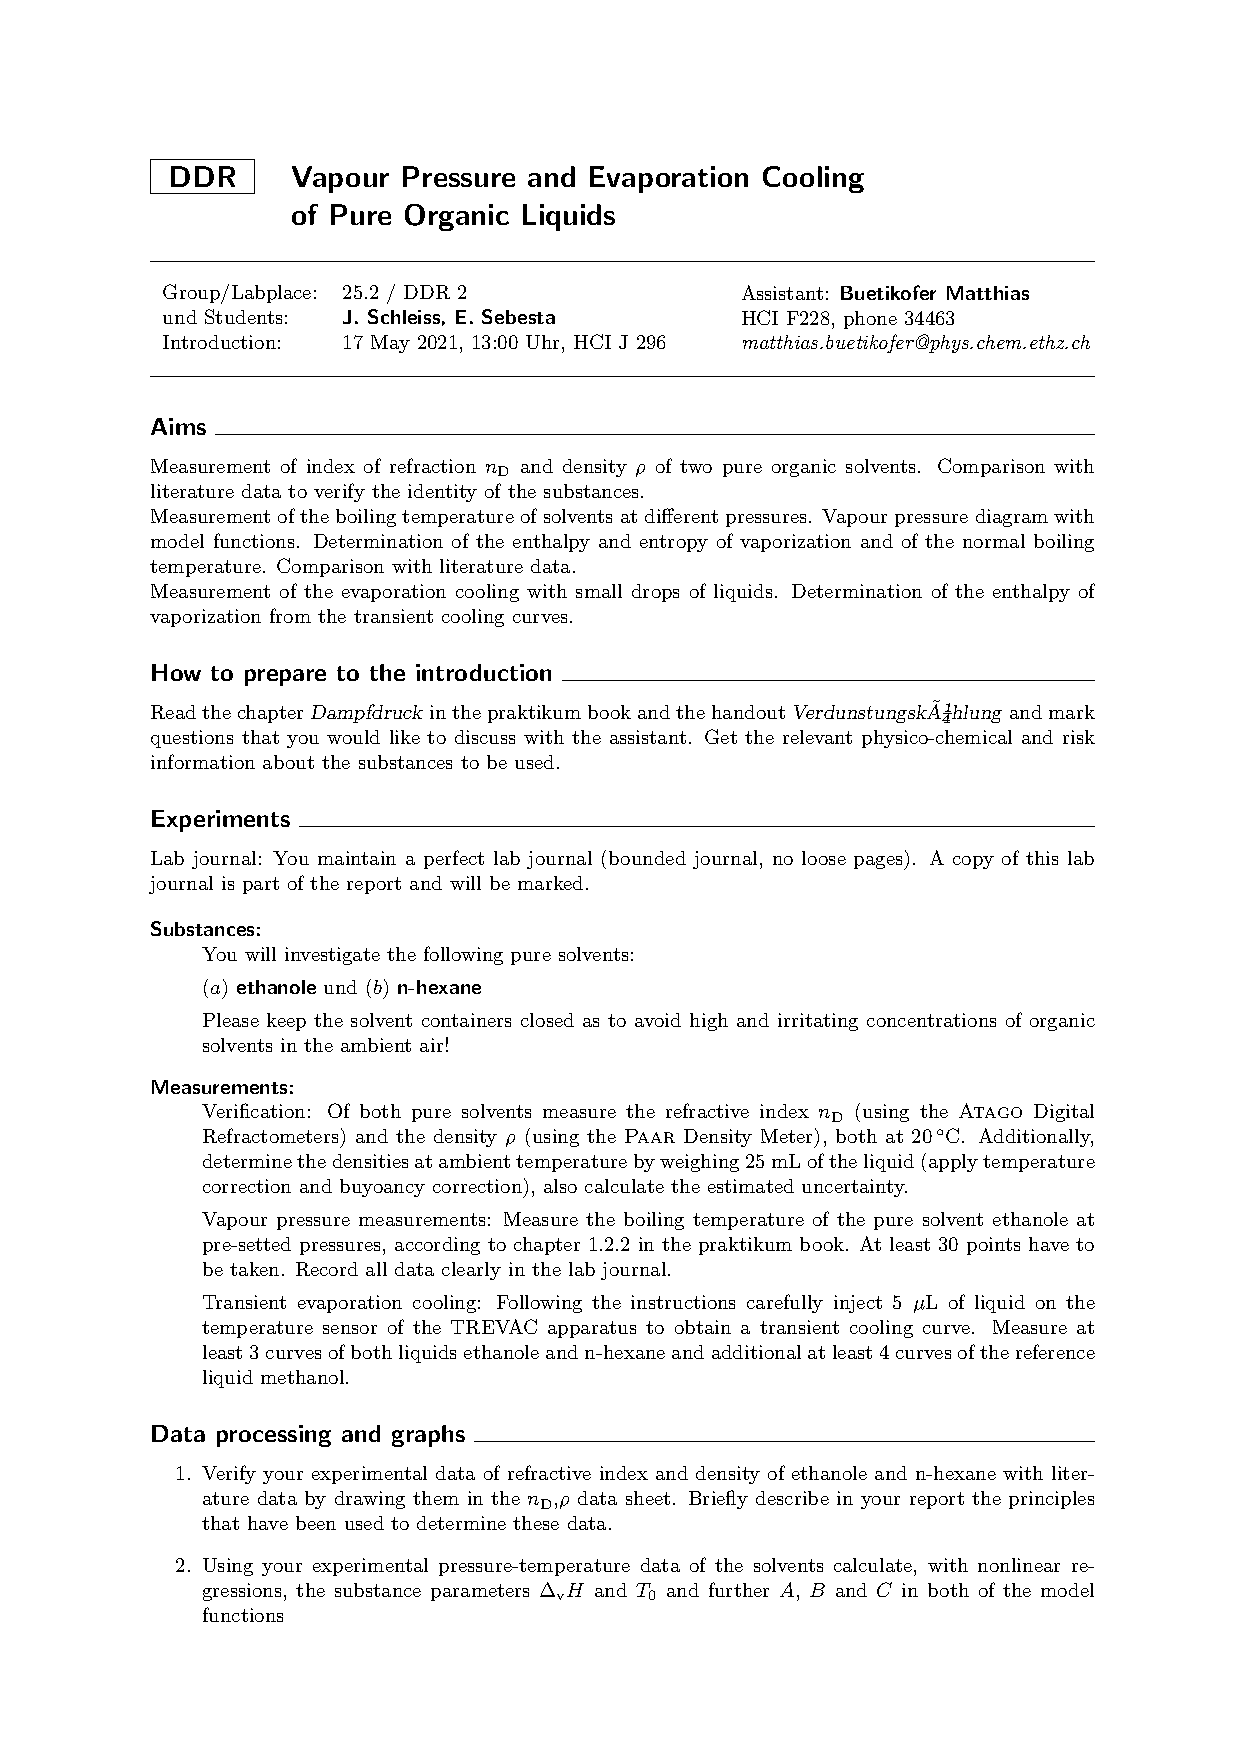
\includegraphics[page = 1,width=\textwidth]{DDRtask.pdf}

\includegraphics[page = 2,width=\textwidth]{DDRtask.pdf}

\subsection*{A4 - Additional Plots}

\begin{figure}[H]
    \centering
    % This file was created by tikzplotlib v0.9.8.
\begin{tikzpicture}

\definecolor{color0}{rgb}{0.12156862745098,0.466666666666667,0.705882352941177}

\begin{axis}[
tick align=outside,
tick pos=left,
x grid style={white!69.0196078431373!black},
width=\textwidth,
height=7cm,
xlabel={time / s},
xmin=-9.58, xmax=201.18,
xtick style={color=black},
y grid style={white!69.0196078431373!black},
ylabel={$\theta$ / C$^{\circ}$},
ymin=31.1025175, ymax=34.7688725,
ytick style={color=black}
]
\path [draw=blue, fill=blue]
(axis cs:25.2,34.59735)
--(axis cs:25.2,34.59735)
--(axis cs:25.4,34.59735)
--(axis cs:25.6,34.59735)
--(axis cs:25.8,34.59735)
--(axis cs:26,34.59735)
--(axis cs:26.2,34.59735)
--(axis cs:26.4,34.59735)
--(axis cs:26.6,34.59735)
--(axis cs:26.8,34.59735)
--(axis cs:27,34.59735)
--(axis cs:27.2,34.59735)
--(axis cs:27.4,34.59735)
--(axis cs:27.6,34.59735)
--(axis cs:27.8,34.59735)
--(axis cs:28,34.59735)
--(axis cs:28.2,34.59735)
--(axis cs:28.4,34.59735)
--(axis cs:28.6,34.59735)
--(axis cs:28.8,34.59735)
--(axis cs:29,34.59735)
--(axis cs:29.2,34.59735)
--(axis cs:29.4,34.59735)
--(axis cs:29.6,34.59735)
--(axis cs:29.8,34.59735)
--(axis cs:30,34.59735)
--(axis cs:30.2,34.59735)
--(axis cs:30.4,34.59735)
--(axis cs:30.6,34.59735)
--(axis cs:30.8,34.59735)
--(axis cs:31,34.59735)
--(axis cs:31.2,34.59735)
--(axis cs:31.4,34.59735)
--(axis cs:31.6,34.59735)
--(axis cs:31.8,34.59735)
--(axis cs:32,34.59735)
--(axis cs:32.2,34.59735)
--(axis cs:32.4,34.59735)
--(axis cs:32.6,34.59735)
--(axis cs:32.8,34.59735)
--(axis cs:33,34.59735)
--(axis cs:33.2,34.59735)
--(axis cs:33.4,34.59735)
--(axis cs:33.6,34.59735)
--(axis cs:33.8,34.59735)
--(axis cs:34,34.59735)
--(axis cs:34.2,34.59735)
--(axis cs:34.4,34.59735)
--(axis cs:34.6,34.59735)
--(axis cs:34.8,34.59735)
--(axis cs:35,34.59735)
--(axis cs:35.2,34.59735)
--(axis cs:35.4,34.59735)
--(axis cs:35.6,34.59735)
--(axis cs:35.8,34.59735)
--(axis cs:36,34.59735)
--(axis cs:36.2,34.59735)
--(axis cs:36.4,34.59735)
--(axis cs:36.6,34.59735)
--(axis cs:36.8,34.59735)
--(axis cs:37,34.59735)
--(axis cs:37.2,34.59735)
--(axis cs:37.4,34.59735)
--(axis cs:37.6,34.59735)
--(axis cs:37.8,34.59735)
--(axis cs:38,34.59735)
--(axis cs:38.2,34.59735)
--(axis cs:38.4,34.59735)
--(axis cs:38.6,34.59735)
--(axis cs:38.8,34.59735)
--(axis cs:39,34.59735)
--(axis cs:39.2,34.59735)
--(axis cs:39.4,34.59735)
--(axis cs:39.6,34.59735)
--(axis cs:39.8,34.59735)
--(axis cs:40,34.59735)
--(axis cs:40.2,34.59735)
--(axis cs:40.4,34.59735)
--(axis cs:40.6,34.59735)
--(axis cs:40.8,34.59735)
--(axis cs:41,34.59735)
--(axis cs:41.2,34.59735)
--(axis cs:41.4,34.59735)
--(axis cs:41.6,34.59735)
--(axis cs:41.8,34.59735)
--(axis cs:42,34.59735)
--(axis cs:42.2,34.59735)
--(axis cs:42.4,34.59735)
--(axis cs:42.6,34.59735)
--(axis cs:42.8,34.59735)
--(axis cs:43,34.59735)
--(axis cs:43.2,34.59735)
--(axis cs:43.4,34.59735)
--(axis cs:43.6,34.59735)
--(axis cs:43.8,34.59735)
--(axis cs:44,34.59735)
--(axis cs:44.2,34.59735)
--(axis cs:44.4,34.59735)
--(axis cs:44.6,34.59735)
--(axis cs:44.8,34.59735)
--(axis cs:45,34.59735)
--(axis cs:45.2,34.59735)
--(axis cs:45.4,34.59735)
--(axis cs:45.6,34.59735)
--(axis cs:45.8,34.59735)
--(axis cs:46,34.59735)
--(axis cs:46.2,34.59735)
--(axis cs:46.4,34.59735)
--(axis cs:46.6,34.59735)
--(axis cs:46.8,34.59735)
--(axis cs:47,34.59735)
--(axis cs:47.2,34.59735)
--(axis cs:47.4,34.59735)
--(axis cs:47.6,34.59735)
--(axis cs:47.8,34.59735)
--(axis cs:48,34.59735)
--(axis cs:48.2,34.59735)
--(axis cs:48.4,34.59735)
--(axis cs:48.6,34.59735)
--(axis cs:48.8,34.59735)
--(axis cs:49,34.59735)
--(axis cs:49.2,34.59735)
--(axis cs:49.4,34.59735)
--(axis cs:49.6,34.59735)
--(axis cs:49.8,34.59735)
--(axis cs:50,34.59735)
--(axis cs:50.2,34.59735)
--(axis cs:50.4,34.59735)
--(axis cs:50.6,34.59735)
--(axis cs:50.8,34.59735)
--(axis cs:51,34.59735)
--(axis cs:51.2,34.59735)
--(axis cs:51.4,34.59735)
--(axis cs:51.6,34.59735)
--(axis cs:51.8,34.59735)
--(axis cs:52,34.59735)
--(axis cs:52.2,34.59735)
--(axis cs:52.4,34.59735)
--(axis cs:52.6,34.59735)
--(axis cs:52.8,34.59735)
--(axis cs:53,34.59735)
--(axis cs:53.2,34.59735)
--(axis cs:53.4,34.59735)
--(axis cs:53.6,34.59735)
--(axis cs:53.8,34.59735)
--(axis cs:54,34.59735)
--(axis cs:54.2,34.59735)
--(axis cs:54.4,34.59735)
--(axis cs:54.6,34.59735)
--(axis cs:54.8,34.59735)
--(axis cs:55,34.59735)
--(axis cs:55.2,34.59735)
--(axis cs:55.4,34.59735)
--(axis cs:55.6,34.59735)
--(axis cs:55.8,34.59735)
--(axis cs:56,34.59735)
--(axis cs:56.2,34.59735)
--(axis cs:56.4,34.59735)
--(axis cs:56.6,34.59735)
--(axis cs:56.8,34.59735)
--(axis cs:57,34.59735)
--(axis cs:57.2,34.59735)
--(axis cs:57.4,34.59735)
--(axis cs:57.6,34.59735)
--(axis cs:57.8,34.59735)
--(axis cs:58,34.59735)
--(axis cs:58.2,34.59735)
--(axis cs:58.4,34.59735)
--(axis cs:58.6,34.59735)
--(axis cs:58.8,34.59735)
--(axis cs:59,34.59735)
--(axis cs:59.2,34.59735)
--(axis cs:59.4,34.59735)
--(axis cs:59.6,34.59735)
--(axis cs:59.8,34.59735)
--(axis cs:60,34.59735)
--(axis cs:60.2,34.59735)
--(axis cs:60.4,34.59735)
--(axis cs:60.6,34.59735)
--(axis cs:60.8,34.59735)
--(axis cs:61,34.59735)
--(axis cs:61.2,34.59735)
--(axis cs:61.4,34.59735)
--(axis cs:61.6,34.59735)
--(axis cs:61.8,34.59735)
--(axis cs:62,34.59735)
--(axis cs:62.2,34.59735)
--(axis cs:62.4,34.59735)
--(axis cs:62.6,34.59735)
--(axis cs:62.8,34.59735)
--(axis cs:63,34.59735)
--(axis cs:63.2,34.59735)
--(axis cs:63.4,34.59735)
--(axis cs:63.6,34.59735)
--(axis cs:63.8,34.59735)
--(axis cs:64,34.59735)
--(axis cs:64.2,34.59735)
--(axis cs:64.4,34.59735)
--(axis cs:64.6,34.59735)
--(axis cs:64.8,34.59735)
--(axis cs:65,34.59735)
--(axis cs:65.2,34.59735)
--(axis cs:65.4,34.59735)
--(axis cs:65.6,34.59735)
--(axis cs:65.8,34.59735)
--(axis cs:66,34.59735)
--(axis cs:66.2,34.59735)
--(axis cs:66.2,34.57976)
--(axis cs:66.2,34.57976)
--(axis cs:66,34.57879)
--(axis cs:65.8,34.57814)
--(axis cs:65.6,34.57735)
--(axis cs:65.4,34.57642)
--(axis cs:65.2,34.57548)
--(axis cs:65,34.5748)
--(axis cs:64.8,34.57399)
--(axis cs:64.6,34.5733)
--(axis cs:64.4,34.57252)
--(axis cs:64.2,34.57148)
--(axis cs:64,34.57024)
--(axis cs:63.8,34.56977)
--(axis cs:63.6,34.56864)
--(axis cs:63.4,34.56797)
--(axis cs:63.2,34.56749)
--(axis cs:63,34.5665)
--(axis cs:62.8,34.56581)
--(axis cs:62.6,34.56497)
--(axis cs:62.4,34.56421)
--(axis cs:62.2,34.56294)
--(axis cs:62,34.56167)
--(axis cs:61.8,34.5603)
--(axis cs:61.6,34.55933)
--(axis cs:61.4,34.55809)
--(axis cs:61.2,34.55658)
--(axis cs:61,34.55479)
--(axis cs:60.8,34.55286)
--(axis cs:60.6,34.55115)
--(axis cs:60.4,34.54947)
--(axis cs:60.2,34.54758)
--(axis cs:60,34.54582)
--(axis cs:59.8,34.54386)
--(axis cs:59.6,34.54163)
--(axis cs:59.4,34.54007)
--(axis cs:59.2,34.53794)
--(axis cs:59,34.53535)
--(axis cs:58.8,34.53293)
--(axis cs:58.6,34.5305)
--(axis cs:58.4,34.5277)
--(axis cs:58.2,34.5245)
--(axis cs:58,34.52188)
--(axis cs:57.8,34.51809)
--(axis cs:57.6,34.51409)
--(axis cs:57.4,34.51008)
--(axis cs:57.2,34.50676)
--(axis cs:57,34.5033)
--(axis cs:56.8,34.49889)
--(axis cs:56.6,34.49445)
--(axis cs:56.4,34.48977)
--(axis cs:56.2,34.48456)
--(axis cs:56,34.47881)
--(axis cs:55.8,34.47359)
--(axis cs:55.6,34.46803)
--(axis cs:55.4,34.46166)
--(axis cs:55.2,34.45571)
--(axis cs:55,34.44848)
--(axis cs:54.8,34.4419)
--(axis cs:54.6,34.43412)
--(axis cs:54.4,34.42653)
--(axis cs:54.2,34.41762)
--(axis cs:54,34.40943)
--(axis cs:53.8,34.40028)
--(axis cs:53.6,34.39014)
--(axis cs:53.4,34.37978)
--(axis cs:53.2,34.36884)
--(axis cs:53,34.3576)
--(axis cs:52.8,34.34525)
--(axis cs:52.6,34.33258)
--(axis cs:52.4,34.31817)
--(axis cs:52.2,34.30383)
--(axis cs:52,34.28838)
--(axis cs:51.8,34.27183)
--(axis cs:51.6,34.25464)
--(axis cs:51.4,34.23599)
--(axis cs:51.2,34.21666)
--(axis cs:51,34.19656)
--(axis cs:50.8,34.17446)
--(axis cs:50.6,34.15204)
--(axis cs:50.4,34.12791)
--(axis cs:50.2,34.10259)
--(axis cs:50,34.07585)
--(axis cs:49.8,34.04757)
--(axis cs:49.6,34.01822)
--(axis cs:49.4,33.98678)
--(axis cs:49.2,33.95242)
--(axis cs:49,33.91687)
--(axis cs:48.8,33.87815)
--(axis cs:48.6,33.83777)
--(axis cs:48.4,33.79514)
--(axis cs:48.2,33.74969)
--(axis cs:48,33.70182)
--(axis cs:47.8,33.65127)
--(axis cs:47.6,33.59714)
--(axis cs:47.4,33.54002)
--(axis cs:47.2,33.47953)
--(axis cs:47,33.41532)
--(axis cs:46.8,33.34734)
--(axis cs:46.6,33.27543)
--(axis cs:46.4,33.19811)
--(axis cs:46.2,33.11747)
--(axis cs:46,33.03086)
--(axis cs:45.8,32.93924)
--(axis cs:45.6,32.84247)
--(axis cs:45.4,32.73927)
--(axis cs:45.2,32.62959)
--(axis cs:45,32.5137)
--(axis cs:44.8,32.39094)
--(axis cs:44.6,32.2615)
--(axis cs:44.4,32.12583)
--(axis cs:44.2,31.98979)
--(axis cs:44,31.86817)
--(axis cs:43.8,31.76402)
--(axis cs:43.6,31.67728)
--(axis cs:43.4,31.60677)
--(axis cs:43.2,31.54661)
--(axis cs:43,31.49409)
--(axis cs:42.8,31.44821)
--(axis cs:42.6,31.40395)
--(axis cs:42.4,31.36428)
--(axis cs:42.2,31.33063)
--(axis cs:42,31.30079)
--(axis cs:41.8,31.28013)
--(axis cs:41.6,31.27183)
--(axis cs:41.4,31.26917)
--(axis cs:41.2,31.27052)
--(axis cs:41,31.27406)
--(axis cs:40.8,31.2812)
--(axis cs:40.6,31.28906)
--(axis cs:40.4,31.29684)
--(axis cs:40.2,31.30486)
--(axis cs:40,31.30876)
--(axis cs:39.8,31.31225)
--(axis cs:39.6,31.32006)
--(axis cs:39.4,31.3255)
--(axis cs:39.2,31.33021)
--(axis cs:39,31.33804)
--(axis cs:38.8,31.34754)
--(axis cs:38.6,31.35873)
--(axis cs:38.4,31.36957)
--(axis cs:38.2,31.37985)
--(axis cs:38,31.39199)
--(axis cs:37.8,31.4012)
--(axis cs:37.6,31.41053)
--(axis cs:37.4,31.42066)
--(axis cs:37.2,31.43334)
--(axis cs:37,31.44575)
--(axis cs:36.8,31.45855)
--(axis cs:36.6,31.47236)
--(axis cs:36.4,31.48854)
--(axis cs:36.2,31.50488)
--(axis cs:36,31.52067)
--(axis cs:35.8,31.53573)
--(axis cs:35.6,31.55307)
--(axis cs:35.4,31.57167)
--(axis cs:35.2,31.59249)
--(axis cs:35,31.61658)
--(axis cs:34.8,31.64193)
--(axis cs:34.6,31.6676)
--(axis cs:34.4,31.69389)
--(axis cs:34.2,31.72206)
--(axis cs:34,31.74936)
--(axis cs:33.8,31.77946)
--(axis cs:33.6,31.81243)
--(axis cs:33.4,31.84697)
--(axis cs:33.2,31.88526)
--(axis cs:33,31.92678)
--(axis cs:32.8,31.97187)
--(axis cs:32.6,32.01887)
--(axis cs:32.4,32.06864)
--(axis cs:32.2,32.12061)
--(axis cs:32,32.17675)
--(axis cs:31.8,32.23538)
--(axis cs:31.6,32.29727)
--(axis cs:31.4,32.36468)
--(axis cs:31.2,32.43573)
--(axis cs:31,32.51313)
--(axis cs:30.8,32.59902)
--(axis cs:30.6,32.69477)
--(axis cs:30.4,32.8007)
--(axis cs:30.2,32.9122)
--(axis cs:30,33.02968)
--(axis cs:29.8,33.15437)
--(axis cs:29.6,33.28972)
--(axis cs:29.4,33.43435)
--(axis cs:29.2,33.58986)
--(axis cs:29,33.75532)
--(axis cs:28.8,33.93439)
--(axis cs:28.6,34.12682)
--(axis cs:28.4,34.32044)
--(axis cs:28.2,34.49924)
--(axis cs:28,34.57249)
--(axis cs:27.8,34.57685)
--(axis cs:27.6,34.57934)
--(axis cs:27.4,34.58206)
--(axis cs:27.2,34.58254)
--(axis cs:27,34.58361)
--(axis cs:26.8,34.58339)
--(axis cs:26.6,34.58413)
--(axis cs:26.4,34.58421)
--(axis cs:26.2,34.58447)
--(axis cs:26,34.58572)
--(axis cs:25.8,34.58851)
--(axis cs:25.6,34.59091)
--(axis cs:25.4,34.59424)
--(axis cs:25.2,34.59735)
--cycle;

\path [draw=blue, fill=blue]
(axis cs:80.6,34.58411)
--(axis cs:80.6,34.58411)
--(axis cs:80.8,34.58411)
--(axis cs:81,34.58411)
--(axis cs:81.2,34.58411)
--(axis cs:81.4,34.58411)
--(axis cs:81.6,34.58411)
--(axis cs:81.8,34.58411)
--(axis cs:82,34.58411)
--(axis cs:82.2,34.58411)
--(axis cs:82.4,34.58411)
--(axis cs:82.6,34.58411)
--(axis cs:82.8,34.58411)
--(axis cs:83,34.58411)
--(axis cs:83.2,34.58411)
--(axis cs:83.4,34.58411)
--(axis cs:83.6,34.58411)
--(axis cs:83.8,34.58411)
--(axis cs:84,34.58411)
--(axis cs:84.2,34.58411)
--(axis cs:84.4,34.58411)
--(axis cs:84.6,34.58411)
--(axis cs:84.8,34.58411)
--(axis cs:85,34.58411)
--(axis cs:85.2,34.58411)
--(axis cs:85.4,34.58411)
--(axis cs:85.6,34.58411)
--(axis cs:85.8,34.58411)
--(axis cs:86,34.58411)
--(axis cs:86.2,34.58411)
--(axis cs:86.4,34.58411)
--(axis cs:86.6,34.58411)
--(axis cs:86.8,34.58411)
--(axis cs:87,34.58411)
--(axis cs:87.2,34.58411)
--(axis cs:87.4,34.58411)
--(axis cs:87.6,34.58411)
--(axis cs:87.8,34.58411)
--(axis cs:88,34.58411)
--(axis cs:88.2,34.58411)
--(axis cs:88.4,34.58411)
--(axis cs:88.6,34.58411)
--(axis cs:88.8,34.58411)
--(axis cs:89,34.58411)
--(axis cs:89.2,34.58411)
--(axis cs:89.4,34.58411)
--(axis cs:89.6,34.58411)
--(axis cs:89.8,34.58411)
--(axis cs:90,34.58411)
--(axis cs:90.2,34.58411)
--(axis cs:90.4,34.58411)
--(axis cs:90.6,34.58411)
--(axis cs:90.8,34.58411)
--(axis cs:91,34.58411)
--(axis cs:91.2,34.58411)
--(axis cs:91.4,34.58411)
--(axis cs:91.6,34.58411)
--(axis cs:91.8,34.58411)
--(axis cs:92,34.58411)
--(axis cs:92.2,34.58411)
--(axis cs:92.4,34.58411)
--(axis cs:92.6,34.58411)
--(axis cs:92.8,34.58411)
--(axis cs:93,34.58411)
--(axis cs:93.2,34.58411)
--(axis cs:93.4,34.58411)
--(axis cs:93.6,34.58411)
--(axis cs:93.8,34.58411)
--(axis cs:94,34.58411)
--(axis cs:94.2,34.58411)
--(axis cs:94.4,34.58411)
--(axis cs:94.6,34.58411)
--(axis cs:94.8,34.58411)
--(axis cs:95,34.58411)
--(axis cs:95.2,34.58411)
--(axis cs:95.4,34.58411)
--(axis cs:95.6,34.58411)
--(axis cs:95.8,34.58411)
--(axis cs:96,34.58411)
--(axis cs:96.2,34.58411)
--(axis cs:96.4,34.58411)
--(axis cs:96.6,34.58411)
--(axis cs:96.8,34.58411)
--(axis cs:97,34.58411)
--(axis cs:97.2,34.58411)
--(axis cs:97.4,34.58411)
--(axis cs:97.6,34.58411)
--(axis cs:97.8,34.58411)
--(axis cs:98,34.58411)
--(axis cs:98.2,34.58411)
--(axis cs:98.4,34.58411)
--(axis cs:98.6,34.58411)
--(axis cs:98.8,34.58411)
--(axis cs:99,34.58411)
--(axis cs:99.2,34.58411)
--(axis cs:99.4,34.58411)
--(axis cs:99.6,34.58411)
--(axis cs:99.8,34.58411)
--(axis cs:100,34.58411)
--(axis cs:100.2,34.58411)
--(axis cs:100.4,34.58411)
--(axis cs:100.6,34.58411)
--(axis cs:100.8,34.58411)
--(axis cs:101,34.58411)
--(axis cs:101.2,34.58411)
--(axis cs:101.4,34.58411)
--(axis cs:101.6,34.58411)
--(axis cs:101.8,34.58411)
--(axis cs:102,34.58411)
--(axis cs:102.2,34.58411)
--(axis cs:102.4,34.58411)
--(axis cs:102.6,34.58411)
--(axis cs:102.8,34.58411)
--(axis cs:103,34.58411)
--(axis cs:103.2,34.58411)
--(axis cs:103.4,34.58411)
--(axis cs:103.6,34.58411)
--(axis cs:103.8,34.58411)
--(axis cs:104,34.58411)
--(axis cs:104.2,34.58411)
--(axis cs:104.4,34.58411)
--(axis cs:104.6,34.58411)
--(axis cs:104.8,34.58411)
--(axis cs:105,34.58411)
--(axis cs:105.2,34.58411)
--(axis cs:105.4,34.58411)
--(axis cs:105.6,34.58411)
--(axis cs:105.8,34.58411)
--(axis cs:106,34.58411)
--(axis cs:106.2,34.58411)
--(axis cs:106.4,34.58411)
--(axis cs:106.6,34.58411)
--(axis cs:106.8,34.58411)
--(axis cs:107,34.58411)
--(axis cs:107.2,34.58411)
--(axis cs:107.4,34.58411)
--(axis cs:107.6,34.58411)
--(axis cs:107.8,34.58411)
--(axis cs:108,34.58411)
--(axis cs:108.2,34.58411)
--(axis cs:108.4,34.58411)
--(axis cs:108.6,34.58411)
--(axis cs:108.8,34.58411)
--(axis cs:109,34.58411)
--(axis cs:109.2,34.58411)
--(axis cs:109.4,34.58411)
--(axis cs:109.6,34.58411)
--(axis cs:109.8,34.58411)
--(axis cs:110,34.58411)
--(axis cs:110.2,34.58411)
--(axis cs:110.4,34.58411)
--(axis cs:110.6,34.58411)
--(axis cs:110.8,34.58411)
--(axis cs:111,34.58411)
--(axis cs:111.2,34.58411)
--(axis cs:111.4,34.58411)
--(axis cs:111.6,34.58411)
--(axis cs:111.8,34.58411)
--(axis cs:112,34.58411)
--(axis cs:112.2,34.58411)
--(axis cs:112.4,34.58411)
--(axis cs:112.6,34.58411)
--(axis cs:112.8,34.58411)
--(axis cs:113,34.58411)
--(axis cs:113.2,34.58411)
--(axis cs:113.4,34.58411)
--(axis cs:113.6,34.58411)
--(axis cs:113.8,34.58411)
--(axis cs:114,34.58411)
--(axis cs:114.2,34.58411)
--(axis cs:114.4,34.58411)
--(axis cs:114.6,34.58411)
--(axis cs:114.8,34.58411)
--(axis cs:115,34.58411)
--(axis cs:115.2,34.58411)
--(axis cs:115.4,34.58411)
--(axis cs:115.6,34.58411)
--(axis cs:115.8,34.58411)
--(axis cs:116,34.58411)
--(axis cs:116.2,34.58411)
--(axis cs:116.4,34.58411)
--(axis cs:116.6,34.58411)
--(axis cs:116.8,34.58411)
--(axis cs:117,34.58411)
--(axis cs:117.2,34.58411)
--(axis cs:117.4,34.58411)
--(axis cs:117.6,34.58411)
--(axis cs:117.8,34.58411)
--(axis cs:118,34.58411)
--(axis cs:118.2,34.58411)
--(axis cs:118.4,34.58411)
--(axis cs:118.6,34.58411)
--(axis cs:118.8,34.58411)
--(axis cs:119,34.58411)
--(axis cs:119.2,34.58411)
--(axis cs:119.4,34.58411)
--(axis cs:119.6,34.58411)
--(axis cs:119.8,34.58411)
--(axis cs:120,34.58411)
--(axis cs:120.2,34.58411)
--(axis cs:120.4,34.58411)
--(axis cs:120.6,34.58411)
--(axis cs:120.8,34.58411)
--(axis cs:121,34.58411)
--(axis cs:121.2,34.58411)
--(axis cs:121.4,34.58411)
--(axis cs:121.6,34.58411)
--(axis cs:121.8,34.58411)
--(axis cs:122,34.58411)
--(axis cs:122.2,34.58411)
--(axis cs:122.4,34.58411)
--(axis cs:122.6,34.58411)
--(axis cs:122.8,34.58411)
--(axis cs:123,34.58411)
--(axis cs:123.2,34.58411)
--(axis cs:123.4,34.58411)
--(axis cs:123.6,34.58411)
--(axis cs:123.8,34.58411)
--(axis cs:123.8,34.57158)
--(axis cs:123.8,34.57158)
--(axis cs:123.6,34.57125)
--(axis cs:123.4,34.57101)
--(axis cs:123.2,34.5708)
--(axis cs:123,34.57037)
--(axis cs:122.8,34.57014)
--(axis cs:122.6,34.56989)
--(axis cs:122.4,34.569)
--(axis cs:122.2,34.56904)
--(axis cs:122,34.56887)
--(axis cs:121.8,34.56839)
--(axis cs:121.6,34.56779)
--(axis cs:121.4,34.56779)
--(axis cs:121.2,34.56729)
--(axis cs:121,34.56694)
--(axis cs:120.8,34.5663)
--(axis cs:120.6,34.56543)
--(axis cs:120.4,34.56455)
--(axis cs:120.2,34.56406)
--(axis cs:120,34.56275)
--(axis cs:119.8,34.56219)
--(axis cs:119.6,34.56125)
--(axis cs:119.4,34.55983)
--(axis cs:119.2,34.55894)
--(axis cs:119,34.55837)
--(axis cs:118.8,34.5569)
--(axis cs:118.6,34.55625)
--(axis cs:118.4,34.55509)
--(axis cs:118.2,34.55438)
--(axis cs:118,34.55318)
--(axis cs:117.8,34.55276)
--(axis cs:117.6,34.55138)
--(axis cs:117.4,34.55021)
--(axis cs:117.2,34.54919)
--(axis cs:117,34.5477)
--(axis cs:116.8,34.54689)
--(axis cs:116.6,34.54493)
--(axis cs:116.4,34.54347)
--(axis cs:116.2,34.54193)
--(axis cs:116,34.54027)
--(axis cs:115.8,34.53856)
--(axis cs:115.6,34.53676)
--(axis cs:115.4,34.53539)
--(axis cs:115.2,34.5336)
--(axis cs:115,34.53211)
--(axis cs:114.8,34.52989)
--(axis cs:114.6,34.52786)
--(axis cs:114.4,34.52584)
--(axis cs:114.2,34.52331)
--(axis cs:114,34.52129)
--(axis cs:113.8,34.51856)
--(axis cs:113.6,34.51607)
--(axis cs:113.4,34.5136)
--(axis cs:113.2,34.51123)
--(axis cs:113,34.50827)
--(axis cs:112.8,34.50557)
--(axis cs:112.6,34.50194)
--(axis cs:112.4,34.4984)
--(axis cs:112.2,34.49547)
--(axis cs:112,34.49182)
--(axis cs:111.8,34.4877)
--(axis cs:111.6,34.4836)
--(axis cs:111.4,34.47949)
--(axis cs:111.2,34.47575)
--(axis cs:111,34.46996)
--(axis cs:110.8,34.46548)
--(axis cs:110.6,34.46017)
--(axis cs:110.4,34.45491)
--(axis cs:110.2,34.44895)
--(axis cs:110,34.44262)
--(axis cs:109.8,34.43594)
--(axis cs:109.6,34.42967)
--(axis cs:109.4,34.4224)
--(axis cs:109.2,34.41463)
--(axis cs:109,34.40578)
--(axis cs:108.8,34.39749)
--(axis cs:108.6,34.3886)
--(axis cs:108.4,34.37916)
--(axis cs:108.2,34.3697)
--(axis cs:108,34.35952)
--(axis cs:107.8,34.34781)
--(axis cs:107.6,34.33677)
--(axis cs:107.4,34.32506)
--(axis cs:107.2,34.3121)
--(axis cs:107,34.29898)
--(axis cs:106.8,34.28516)
--(axis cs:106.6,34.26957)
--(axis cs:106.4,34.25415)
--(axis cs:106.2,34.23647)
--(axis cs:106,34.21935)
--(axis cs:105.8,34.1997)
--(axis cs:105.6,34.17908)
--(axis cs:105.4,34.15784)
--(axis cs:105.2,34.13482)
--(axis cs:105,34.11126)
--(axis cs:104.8,34.08565)
--(axis cs:104.6,34.05875)
--(axis cs:104.4,34.03046)
--(axis cs:104.2,34.00045)
--(axis cs:104,33.9689)
--(axis cs:103.8,33.93561)
--(axis cs:103.6,33.90028)
--(axis cs:103.4,33.8625)
--(axis cs:103.2,33.82259)
--(axis cs:103,33.78063)
--(axis cs:102.8,33.73569)
--(axis cs:102.6,33.6884)
--(axis cs:102.4,33.63818)
--(axis cs:102.2,33.58476)
--(axis cs:102,33.52835)
--(axis cs:101.8,33.46854)
--(axis cs:101.6,33.40459)
--(axis cs:101.4,33.33723)
--(axis cs:101.2,33.26596)
--(axis cs:101,33.19061)
--(axis cs:100.8,33.10957)
--(axis cs:100.6,33.0249)
--(axis cs:100.4,32.93519)
--(axis cs:100.2,32.83918)
--(axis cs:100,32.7376)
--(axis cs:99.8,32.62924)
--(axis cs:99.6,32.51449)
--(axis cs:99.4,32.39299)
--(axis cs:99.2,32.26445)
--(axis cs:99,32.12875)
--(axis cs:98.8,31.99038)
--(axis cs:98.6,31.86075)
--(axis cs:98.4,31.75097)
--(axis cs:98.2,31.65907)
--(axis cs:98,31.58426)
--(axis cs:97.8,31.52383)
--(axis cs:97.6,31.47429)
--(axis cs:97.4,31.42848)
--(axis cs:97.2,31.38371)
--(axis cs:97,31.34368)
--(axis cs:96.8,31.31198)
--(axis cs:96.6,31.28874)
--(axis cs:96.4,31.27712)
--(axis cs:96.2,31.27413)
--(axis cs:96,31.2722)
--(axis cs:95.8,31.27484)
--(axis cs:95.6,31.27988)
--(axis cs:95.4,31.28617)
--(axis cs:95.2,31.29115)
--(axis cs:95,31.29714)
--(axis cs:94.8,31.30574)
--(axis cs:94.6,31.31409)
--(axis cs:94.4,31.31958)
--(axis cs:94.2,31.3265)
--(axis cs:94,31.33184)
--(axis cs:93.8,31.33817)
--(axis cs:93.6,31.34583)
--(axis cs:93.4,31.35582)
--(axis cs:93.2,31.36531)
--(axis cs:93,31.37412)
--(axis cs:92.8,31.38574)
--(axis cs:92.6,31.39827)
--(axis cs:92.4,31.40862)
--(axis cs:92.2,31.41826)
--(axis cs:92,31.42837)
--(axis cs:91.8,31.43734)
--(axis cs:91.6,31.44853)
--(axis cs:91.4,31.46137)
--(axis cs:91.2,31.47671)
--(axis cs:91,31.4926)
--(axis cs:90.8,31.50773)
--(axis cs:90.6,31.52169)
--(axis cs:90.4,31.53746)
--(axis cs:90.2,31.55488)
--(axis cs:90,31.57555)
--(axis cs:89.8,31.59532)
--(axis cs:89.6,31.61395)
--(axis cs:89.4,31.63504)
--(axis cs:89.2,31.65808)
--(axis cs:89,31.68113)
--(axis cs:88.8,31.7064)
--(axis cs:88.6,31.73196)
--(axis cs:88.4,31.76224)
--(axis cs:88.2,31.79471)
--(axis cs:88,31.83099)
--(axis cs:87.8,31.86727)
--(axis cs:87.6,31.91036)
--(axis cs:87.4,31.95453)
--(axis cs:87.2,32.00149)
--(axis cs:87,32.05131)
--(axis cs:86.8,32.1046)
--(axis cs:86.6,32.16206)
--(axis cs:86.4,32.22388)
--(axis cs:86.2,32.28791)
--(axis cs:86,32.35497)
--(axis cs:85.8,32.42661)
--(axis cs:85.6,32.50451)
--(axis cs:85.4,32.58712)
--(axis cs:85.2,32.67661)
--(axis cs:85,32.77019)
--(axis cs:84.8,32.86958)
--(axis cs:84.6,32.9774)
--(axis cs:84.4,33.09479)
--(axis cs:84.2,33.22189)
--(axis cs:84,33.35872)
--(axis cs:83.8,33.50426)
--(axis cs:83.6,33.66143)
--(axis cs:83.4,33.82829)
--(axis cs:83.2,34.00632)
--(axis cs:83,34.18622)
--(axis cs:82.8,34.36457)
--(axis cs:82.6,34.52494)
--(axis cs:82.4,34.56165)
--(axis cs:82.2,34.5664)
--(axis cs:82,34.57055)
--(axis cs:81.8,34.57423)
--(axis cs:81.6,34.57708)
--(axis cs:81.4,34.57823)
--(axis cs:81.2,34.57902)
--(axis cs:81,34.58078)
--(axis cs:80.8,34.58242)
--(axis cs:80.6,34.58411)
--cycle;

\path [draw=blue, fill=blue]
(axis cs:135.6,34.57902)
--(axis cs:135.6,34.57902)
--(axis cs:135.8,34.57902)
--(axis cs:136,34.57902)
--(axis cs:136.2,34.57902)
--(axis cs:136.4,34.57902)
--(axis cs:136.6,34.57902)
--(axis cs:136.8,34.57902)
--(axis cs:137,34.57902)
--(axis cs:137.2,34.57902)
--(axis cs:137.4,34.57902)
--(axis cs:137.6,34.57902)
--(axis cs:137.8,34.57902)
--(axis cs:138,34.57902)
--(axis cs:138.2,34.57902)
--(axis cs:138.4,34.57902)
--(axis cs:138.6,34.57902)
--(axis cs:138.8,34.57902)
--(axis cs:139,34.57902)
--(axis cs:139.2,34.57902)
--(axis cs:139.4,34.57902)
--(axis cs:139.6,34.57902)
--(axis cs:139.8,34.57902)
--(axis cs:140,34.57902)
--(axis cs:140.2,34.57902)
--(axis cs:140.4,34.57902)
--(axis cs:140.6,34.57902)
--(axis cs:140.8,34.57902)
--(axis cs:141,34.57902)
--(axis cs:141.2,34.57902)
--(axis cs:141.4,34.57902)
--(axis cs:141.6,34.57902)
--(axis cs:141.8,34.57902)
--(axis cs:142,34.57902)
--(axis cs:142.2,34.57902)
--(axis cs:142.4,34.57902)
--(axis cs:142.6,34.57902)
--(axis cs:142.8,34.57902)
--(axis cs:143,34.57902)
--(axis cs:143.2,34.57902)
--(axis cs:143.4,34.57902)
--(axis cs:143.6,34.57902)
--(axis cs:143.8,34.57902)
--(axis cs:144,34.57902)
--(axis cs:144.2,34.57902)
--(axis cs:144.4,34.57902)
--(axis cs:144.6,34.57902)
--(axis cs:144.8,34.57902)
--(axis cs:145,34.57902)
--(axis cs:145.2,34.57902)
--(axis cs:145.4,34.57902)
--(axis cs:145.6,34.57902)
--(axis cs:145.8,34.57902)
--(axis cs:146,34.57902)
--(axis cs:146.2,34.57902)
--(axis cs:146.4,34.57902)
--(axis cs:146.6,34.57902)
--(axis cs:146.8,34.57902)
--(axis cs:147,34.57902)
--(axis cs:147.2,34.57902)
--(axis cs:147.4,34.57902)
--(axis cs:147.6,34.57902)
--(axis cs:147.8,34.57902)
--(axis cs:148,34.57902)
--(axis cs:148.2,34.57902)
--(axis cs:148.4,34.57902)
--(axis cs:148.6,34.57902)
--(axis cs:148.8,34.57902)
--(axis cs:149,34.57902)
--(axis cs:149.2,34.57902)
--(axis cs:149.4,34.57902)
--(axis cs:149.6,34.57902)
--(axis cs:149.8,34.57902)
--(axis cs:150,34.57902)
--(axis cs:150.2,34.57902)
--(axis cs:150.4,34.57902)
--(axis cs:150.6,34.57902)
--(axis cs:150.8,34.57902)
--(axis cs:151,34.57902)
--(axis cs:151.2,34.57902)
--(axis cs:151.4,34.57902)
--(axis cs:151.6,34.57902)
--(axis cs:151.8,34.57902)
--(axis cs:152,34.57902)
--(axis cs:152.2,34.57902)
--(axis cs:152.4,34.57902)
--(axis cs:152.6,34.57902)
--(axis cs:152.8,34.57902)
--(axis cs:153,34.57902)
--(axis cs:153.2,34.57902)
--(axis cs:153.4,34.57902)
--(axis cs:153.6,34.57902)
--(axis cs:153.8,34.57902)
--(axis cs:154,34.57902)
--(axis cs:154.2,34.57902)
--(axis cs:154.4,34.57902)
--(axis cs:154.6,34.57902)
--(axis cs:154.8,34.57902)
--(axis cs:155,34.57902)
--(axis cs:155.2,34.57902)
--(axis cs:155.4,34.57902)
--(axis cs:155.6,34.57902)
--(axis cs:155.8,34.57902)
--(axis cs:156,34.57902)
--(axis cs:156.2,34.57902)
--(axis cs:156.4,34.57902)
--(axis cs:156.6,34.57902)
--(axis cs:156.8,34.57902)
--(axis cs:157,34.57902)
--(axis cs:157.2,34.57902)
--(axis cs:157.4,34.57902)
--(axis cs:157.6,34.57902)
--(axis cs:157.8,34.57902)
--(axis cs:158,34.57902)
--(axis cs:158.2,34.57902)
--(axis cs:158.4,34.57902)
--(axis cs:158.6,34.57902)
--(axis cs:158.8,34.57902)
--(axis cs:159,34.57902)
--(axis cs:159.2,34.57902)
--(axis cs:159.4,34.57902)
--(axis cs:159.6,34.57902)
--(axis cs:159.8,34.57902)
--(axis cs:160,34.57902)
--(axis cs:160.2,34.57902)
--(axis cs:160.4,34.57902)
--(axis cs:160.6,34.57902)
--(axis cs:160.8,34.57902)
--(axis cs:161,34.57902)
--(axis cs:161.2,34.57902)
--(axis cs:161.4,34.57902)
--(axis cs:161.6,34.57902)
--(axis cs:161.8,34.57902)
--(axis cs:162,34.57902)
--(axis cs:162.2,34.57902)
--(axis cs:162.4,34.57902)
--(axis cs:162.6,34.57902)
--(axis cs:162.8,34.57902)
--(axis cs:163,34.57902)
--(axis cs:163.2,34.57902)
--(axis cs:163.4,34.57902)
--(axis cs:163.6,34.57902)
--(axis cs:163.8,34.57902)
--(axis cs:164,34.57902)
--(axis cs:164.2,34.57902)
--(axis cs:164.4,34.57902)
--(axis cs:164.6,34.57902)
--(axis cs:164.8,34.57902)
--(axis cs:165,34.57902)
--(axis cs:165.2,34.57902)
--(axis cs:165.4,34.57902)
--(axis cs:165.6,34.57902)
--(axis cs:165.8,34.57902)
--(axis cs:166,34.57902)
--(axis cs:166.2,34.57902)
--(axis cs:166.4,34.57902)
--(axis cs:166.6,34.57902)
--(axis cs:166.8,34.57902)
--(axis cs:167,34.57902)
--(axis cs:167.2,34.57902)
--(axis cs:167.4,34.57902)
--(axis cs:167.6,34.57902)
--(axis cs:167.8,34.57902)
--(axis cs:168,34.57902)
--(axis cs:168.2,34.57902)
--(axis cs:168.4,34.57902)
--(axis cs:168.6,34.57902)
--(axis cs:168.8,34.57902)
--(axis cs:169,34.57902)
--(axis cs:169.2,34.57902)
--(axis cs:169.4,34.57902)
--(axis cs:169.6,34.57902)
--(axis cs:169.8,34.57902)
--(axis cs:170,34.57902)
--(axis cs:170.2,34.57902)
--(axis cs:170.4,34.57902)
--(axis cs:170.6,34.57902)
--(axis cs:170.8,34.57902)
--(axis cs:171,34.57902)
--(axis cs:171.2,34.57902)
--(axis cs:171.4,34.57902)
--(axis cs:171.6,34.57902)
--(axis cs:171.8,34.57902)
--(axis cs:172,34.57902)
--(axis cs:172.2,34.57902)
--(axis cs:172.4,34.57902)
--(axis cs:172.6,34.57902)
--(axis cs:172.8,34.57902)
--(axis cs:173,34.57902)
--(axis cs:173.2,34.57902)
--(axis cs:173.4,34.57902)
--(axis cs:173.6,34.57902)
--(axis cs:173.8,34.57902)
--(axis cs:174,34.57902)
--(axis cs:174.2,34.57902)
--(axis cs:174.4,34.57902)
--(axis cs:174.6,34.57902)
--(axis cs:174.8,34.57902)
--(axis cs:175,34.57902)
--(axis cs:175.2,34.57902)
--(axis cs:175.4,34.57902)
--(axis cs:175.6,34.57902)
--(axis cs:175.8,34.57902)
--(axis cs:176,34.57902)
--(axis cs:176.2,34.57902)
--(axis cs:176.4,34.57902)
--(axis cs:176.6,34.57902)
--(axis cs:176.8,34.57902)
--(axis cs:177,34.57902)
--(axis cs:177.2,34.57902)
--(axis cs:177.4,34.57902)
--(axis cs:177.6,34.57902)
--(axis cs:177.8,34.57902)
--(axis cs:178,34.57902)
--(axis cs:178.2,34.57902)
--(axis cs:178.4,34.57902)
--(axis cs:178.6,34.57902)
--(axis cs:178.8,34.57902)
--(axis cs:179,34.57902)
--(axis cs:179.2,34.57902)
--(axis cs:179.4,34.57902)
--(axis cs:179.4,34.57994)
--(axis cs:179.4,34.57994)
--(axis cs:179.2,34.5801)
--(axis cs:179,34.57937)
--(axis cs:178.8,34.57902)
--(axis cs:178.6,34.57869)
--(axis cs:178.4,34.57843)
--(axis cs:178.2,34.57873)
--(axis cs:178,34.57898)
--(axis cs:177.8,34.57902)
--(axis cs:177.6,34.57837)
--(axis cs:177.4,34.57884)
--(axis cs:177.2,34.57806)
--(axis cs:177,34.57694)
--(axis cs:176.8,34.57757)
--(axis cs:176.6,34.5778)
--(axis cs:176.4,34.57665)
--(axis cs:176.2,34.57633)
--(axis cs:176,34.57561)
--(axis cs:175.8,34.575)
--(axis cs:175.6,34.57519)
--(axis cs:175.4,34.57487)
--(axis cs:175.2,34.57414)
--(axis cs:175,34.57334)
--(axis cs:174.8,34.57321)
--(axis cs:174.6,34.57253)
--(axis cs:174.4,34.57156)
--(axis cs:174.2,34.57111)
--(axis cs:174,34.57149)
--(axis cs:173.8,34.57159)
--(axis cs:173.6,34.57031)
--(axis cs:173.4,34.56997)
--(axis cs:173.2,34.56826)
--(axis cs:173,34.5685)
--(axis cs:172.8,34.56778)
--(axis cs:172.6,34.56669)
--(axis cs:172.4,34.5654)
--(axis cs:172.2,34.56494)
--(axis cs:172,34.56427)
--(axis cs:171.8,34.56271)
--(axis cs:171.6,34.56221)
--(axis cs:171.4,34.56077)
--(axis cs:171.2,34.55936)
--(axis cs:171,34.55825)
--(axis cs:170.8,34.55732)
--(axis cs:170.6,34.55604)
--(axis cs:170.4,34.55459)
--(axis cs:170.2,34.55366)
--(axis cs:170,34.55214)
--(axis cs:169.8,34.55016)
--(axis cs:169.6,34.54857)
--(axis cs:169.4,34.54706)
--(axis cs:169.2,34.54567)
--(axis cs:169,34.54403)
--(axis cs:168.8,34.54214)
--(axis cs:168.6,34.53984)
--(axis cs:168.4,34.53787)
--(axis cs:168.2,34.53576)
--(axis cs:168,34.53401)
--(axis cs:167.8,34.53092)
--(axis cs:167.6,34.52791)
--(axis cs:167.4,34.52578)
--(axis cs:167.2,34.52287)
--(axis cs:167,34.52003)
--(axis cs:166.8,34.51664)
--(axis cs:166.6,34.51346)
--(axis cs:166.4,34.50949)
--(axis cs:166.2,34.50676)
--(axis cs:166,34.5031)
--(axis cs:165.8,34.49892)
--(axis cs:165.6,34.49498)
--(axis cs:165.4,34.49095)
--(axis cs:165.2,34.48616)
--(axis cs:165,34.48133)
--(axis cs:164.8,34.47671)
--(axis cs:164.6,34.47156)
--(axis cs:164.4,34.46624)
--(axis cs:164.2,34.46101)
--(axis cs:164,34.45501)
--(axis cs:163.8,34.44832)
--(axis cs:163.6,34.44187)
--(axis cs:163.4,34.43525)
--(axis cs:163.2,34.42834)
--(axis cs:163,34.42007)
--(axis cs:162.8,34.41175)
--(axis cs:162.6,34.40277)
--(axis cs:162.4,34.39405)
--(axis cs:162.2,34.38366)
--(axis cs:162,34.37319)
--(axis cs:161.8,34.36203)
--(axis cs:161.6,34.35093)
--(axis cs:161.4,34.33916)
--(axis cs:161.2,34.3259)
--(axis cs:161,34.31308)
--(axis cs:160.8,34.29928)
--(axis cs:160.6,34.28466)
--(axis cs:160.4,34.26881)
--(axis cs:160.2,34.25214)
--(axis cs:160,34.23426)
--(axis cs:159.8,34.21538)
--(axis cs:159.6,34.19561)
--(axis cs:159.4,34.17395)
--(axis cs:159.2,34.15193)
--(axis cs:159,34.12776)
--(axis cs:158.8,34.10274)
--(axis cs:158.6,34.07554)
--(axis cs:158.4,34.04765)
--(axis cs:158.2,34.01756)
--(axis cs:158,33.98515)
--(axis cs:157.8,33.95176)
--(axis cs:157.6,33.91588)
--(axis cs:157.4,33.87868)
--(axis cs:157.2,33.83934)
--(axis cs:157,33.79636)
--(axis cs:156.8,33.75233)
--(axis cs:156.6,33.70465)
--(axis cs:156.4,33.65333)
--(axis cs:156.2,33.60014)
--(axis cs:156,33.54362)
--(axis cs:155.8,33.48341)
--(axis cs:155.6,33.41958)
--(axis cs:155.4,33.3522)
--(axis cs:155.2,33.28059)
--(axis cs:155,33.20469)
--(axis cs:154.8,33.12388)
--(axis cs:154.6,33.0383)
--(axis cs:154.4,32.9471)
--(axis cs:154.2,32.85078)
--(axis cs:154,32.74922)
--(axis cs:153.8,32.64053)
--(axis cs:153.6,32.52593)
--(axis cs:153.4,32.40363)
--(axis cs:153.2,32.27421)
--(axis cs:153,32.13947)
--(axis cs:152.8,32.00349)
--(axis cs:152.6,31.87941)
--(axis cs:152.4,31.7745)
--(axis cs:152.2,31.68795)
--(axis cs:152,31.61426)
--(axis cs:151.8,31.55082)
--(axis cs:151.6,31.49791)
--(axis cs:151.4,31.44872)
--(axis cs:151.2,31.40181)
--(axis cs:151,31.35869)
--(axis cs:150.8,31.32563)
--(axis cs:150.6,31.30084)
--(axis cs:150.4,31.28433)
--(axis cs:150.2,31.2767)
--(axis cs:150,31.27493)
--(axis cs:149.8,31.28194)
--(axis cs:149.6,31.28754)
--(axis cs:149.4,31.29078)
--(axis cs:149.2,31.29497)
--(axis cs:149,31.30268)
--(axis cs:148.8,31.30806)
--(axis cs:148.6,31.31501)
--(axis cs:148.4,31.32322)
--(axis cs:148.2,31.3334)
--(axis cs:148,31.34165)
--(axis cs:147.8,31.35059)
--(axis cs:147.6,31.35977)
--(axis cs:147.4,31.36749)
--(axis cs:147.2,31.37803)
--(axis cs:147,31.38798)
--(axis cs:146.8,31.39479)
--(axis cs:146.6,31.40239)
--(axis cs:146.4,31.41022)
--(axis cs:146.2,31.42008)
--(axis cs:146,31.42985)
--(axis cs:145.8,31.44139)
--(axis cs:145.6,31.45368)
--(axis cs:145.4,31.46736)
--(axis cs:145.2,31.48008)
--(axis cs:145,31.49428)
--(axis cs:144.8,31.50878)
--(axis cs:144.6,31.52807)
--(axis cs:144.4,31.54986)
--(axis cs:144.2,31.57383)
--(axis cs:144,31.59824)
--(axis cs:143.8,31.62113)
--(axis cs:143.6,31.64611)
--(axis cs:143.4,31.67174)
--(axis cs:143.2,31.69989)
--(axis cs:143,31.73087)
--(axis cs:142.8,31.76291)
--(axis cs:142.6,31.79668)
--(axis cs:142.4,31.83265)
--(axis cs:142.2,31.87048)
--(axis cs:142,31.90975)
--(axis cs:141.8,31.95207)
--(axis cs:141.6,31.9968)
--(axis cs:141.4,32.04259)
--(axis cs:141.2,32.09011)
--(axis cs:141,32.14291)
--(axis cs:140.8,32.20045)
--(axis cs:140.6,32.26234)
--(axis cs:140.4,32.32784)
--(axis cs:140.2,32.39748)
--(axis cs:140,32.47161)
--(axis cs:139.8,32.55166)
--(axis cs:139.6,32.63751)
--(axis cs:139.4,32.72969)
--(axis cs:139.2,32.82943)
--(axis cs:139,32.94078)
--(axis cs:138.8,33.0605)
--(axis cs:138.6,33.18853)
--(axis cs:138.4,33.32616)
--(axis cs:138.2,33.47213)
--(axis cs:138,33.62482)
--(axis cs:137.8,33.78306)
--(axis cs:137.6,33.94416)
--(axis cs:137.4,34.08679)
--(axis cs:137.2,34.20783)
--(axis cs:137,34.3172)
--(axis cs:136.8,34.40571)
--(axis cs:136.6,34.47476)
--(axis cs:136.4,34.5313)
--(axis cs:136.2,34.56905)
--(axis cs:136,34.57711)
--(axis cs:135.8,34.57816)
--(axis cs:135.6,34.57902)
--cycle;

\addplot [semithick, color0]
table {%
0 34.601
0.200000000000003 34.60076
0.399999999999999 34.60031
0.600000000000001 34.5996
0.799999999999997 34.59976
1 34.60015
1.2 34.60016
1.4 34.5999
1.6 34.60077
1.8 34.60051
2 34.60046
2.2 34.60012
2.4 34.60061
2.6 34.60042
2.8 34.59976
3 34.59943
3.2 34.59979
3.4 34.59905
3.6 34.59937
3.8 34.59909
4 34.59972
4.2 34.59965
4.4 34.59982
4.6 34.59989
4.8 34.60042
5 34.60103
5.2 34.60117
5.4 34.60048
5.6 34.60111
5.8 34.60112
6 34.60048
6.2 34.59938
6.4 34.59878
6.6 34.59891
6.8 34.59891
7 34.59947
7.2 34.59902
7.4 34.59903
7.6 34.59896
7.8 34.59896
8 34.59875
8.2 34.59785
8.4 34.59887
8.6 34.59884
8.8 34.59861
9 34.59892
9.2 34.5989
9.4 34.59873
9.6 34.59934
9.8 34.59915
10 34.59913
10.2 34.59894
10.4 34.59888
10.6 34.59909
10.8 34.59825
11 34.59865
11.2 34.59849
11.4 34.59853
11.6 34.59799
11.8 34.59807
12 34.59865
12.2 34.59887
12.4 34.59893
12.6 34.59909
12.8 34.59862
13 34.59871
13.2 34.59848
13.4 34.59947
13.6 34.59931
13.8 34.5998
14 34.59991
14.2 34.60019
14.4 34.5997
14.6 34.59942
14.8 34.59977
15 34.59962
15.2 34.59948
15.4 34.6001
15.6 34.59931
15.8 34.5991
16 34.59928
16.2 34.59951
16.4 34.5992
16.6 34.5989
16.8 34.59887
17 34.59954
17.2 34.59901
17.4 34.59884
17.6 34.59933
17.8 34.59968
18 34.59906
18.2 34.59937
18.4 34.59912
18.6 34.59854
18.8 34.59881
19 34.5987
19.2 34.59915
19.4 34.59944
19.6 34.59946
19.8 34.60021
20 34.60054
20.2 34.60128
20.4 34.60148
20.6 34.60162
20.8 34.60125
21 34.60105
21.2 34.60077
21.4 34.60062
21.6 34.60064
21.8 34.60071
22 34.60112
22.2 34.60047
22.4 34.60058
22.6 34.6006
22.8 34.60105
23 34.60092
23.2 34.60148
23.4 34.60207
23.6 34.60159
23.8 34.60207
24 34.60222
24.2 34.60199
24.4 34.60138
24.6 34.60181
24.8 34.60142
25 34.60076
25.2 34.59735
25.4 34.59424
25.6 34.59091
25.8 34.58851
26 34.58572
26.2 34.58447
26.4 34.58421
26.6 34.58413
26.8 34.58339
27 34.58361
27.2 34.58254
27.4 34.58206
27.6 34.57934
27.8 34.57685
28 34.57249
28.2 34.49924
28.4 34.32044
28.6 34.12682
28.8 33.93439
29 33.75532
29.2 33.58986
29.4 33.43435
29.6 33.28972
29.8 33.15437
30 33.02968
30.2 32.9122
30.4 32.8007
30.6 32.69477
30.8 32.59902
31 32.51313
31.2 32.43573
31.4 32.36468
31.6 32.29727
31.8 32.23538
32 32.17675
32.2 32.12061
32.4 32.06864
32.6 32.01887
32.8 31.97187
33 31.92678
33.2 31.88526
33.4 31.84697
33.6 31.81243
33.8 31.77946
34 31.74936
34.2 31.72206
34.4 31.69389
34.6 31.6676
34.8 31.64193
35 31.61658
35.2 31.59249
35.4 31.57167
35.6 31.55307
35.8 31.53573
36 31.52067
36.2 31.50488
36.4 31.48854
36.6 31.47236
36.8 31.45855
37 31.44575
37.2 31.43334
37.4 31.42066
37.6 31.41053
37.8 31.4012
38 31.39199
38.2 31.37985
38.4 31.36957
38.6 31.35873
38.8 31.34754
39 31.33804
39.2 31.33021
39.4 31.3255
39.6 31.32006
39.8 31.31225
40 31.30876
40.2 31.30486
40.4 31.29684
40.6 31.28906
40.8 31.2812
41 31.27406
41.2 31.27052
41.4 31.26917
41.6 31.27183
41.8 31.28013
42 31.30079
42.2 31.33063
42.4 31.36428
42.6 31.40395
42.8 31.44821
43 31.49409
43.2 31.54661
43.4 31.60677
43.6 31.67728
43.8 31.76402
44 31.86817
44.2 31.98979
44.4 32.12583
44.6 32.2615
44.8 32.39094
45 32.5137
45.2 32.62959
45.4 32.73927
45.6 32.84247
45.8 32.93924
46 33.03086
46.2 33.11747
46.4 33.19811
46.6 33.27543
46.8 33.34734
47 33.41532
47.2 33.47953
47.4 33.54002
47.6 33.59714
47.8 33.65127
48 33.70182
48.2 33.74969
48.4 33.79514
48.6 33.83777
48.8 33.87815
49 33.91687
49.2 33.95242
49.4 33.98678
49.6 34.01822
49.8 34.04757
50 34.07585
50.2 34.10259
50.4 34.12791
50.6 34.15204
50.8 34.17446
51 34.19656
51.2 34.21666
51.4 34.23599
51.6 34.25464
51.8 34.27183
52 34.28838
52.2 34.30383
52.4 34.31817
52.6 34.33258
52.8 34.34525
53 34.3576
53.2 34.36884
53.4 34.37978
53.6 34.39014
53.8 34.40028
54 34.40943
54.2 34.41762
54.4 34.42653
54.6 34.43412
54.8 34.4419
55 34.44848
55.2 34.45571
55.4 34.46166
55.6 34.46803
55.8 34.47359
56 34.47881
56.2 34.48456
56.4 34.48977
56.6 34.49445
56.8 34.49889
57 34.5033
57.2 34.50676
57.4 34.51008
57.6 34.51409
57.8 34.51809
58 34.52188
58.2 34.5245
58.4 34.5277
58.6 34.5305
58.8 34.53293
59 34.53535
59.2 34.53794
59.4 34.54007
59.6 34.54163
59.8 34.54386
60 34.54582
60.2 34.54758
60.4 34.54947
60.6 34.55115
60.8 34.55286
61 34.55479
61.2 34.55658
61.4 34.55809
61.6 34.55933
61.8 34.5603
62 34.56167
62.2 34.56294
62.4 34.56421
62.6 34.56497
62.8 34.56581
63 34.5665
63.2 34.56749
63.4 34.56797
63.6 34.56864
63.8 34.56977
64 34.57024
64.2 34.57148
64.4 34.57252
64.6 34.5733
64.8 34.57399
65 34.5748
65.2 34.57548
65.4 34.57642
65.6 34.57735
65.8 34.57814
66 34.57879
66.2 34.57976
66.4 34.58034
66.6 34.58081
66.8 34.58134
67 34.58178
67.2 34.58192
67.4 34.5821
67.6 34.58203
67.8 34.58296
68 34.58282
68.2 34.58233
68.4 34.58263
68.6 34.58326
68.8 34.58411
69 34.58429
69.2 34.58426
69.4 34.58464
69.6 34.58456
69.8 34.58458
70 34.58504
70.2 34.58499
70.4 34.58527
70.6 34.58501
70.8 34.58534
71 34.58548
71.2 34.58587
71.4 34.58605
71.6 34.58591
71.8 34.58637
72 34.58648
72.2 34.58744
72.4 34.58705
72.6 34.58715
72.8 34.58717
73 34.58705
73.2 34.58721
73.4 34.58702
73.6 34.58667
73.8 34.58709
74 34.58707
74.2 34.58648
74.4 34.58717
74.6 34.58755
74.8 34.58734
75 34.58755
75.2 34.58791
75.4 34.58834
75.6 34.58879
75.8 34.58816
76 34.58841
76.2 34.58808
76.4 34.58798
76.6 34.58906
76.8 34.58856
77 34.58877
77.2 34.58839
77.4 34.5894
77.6 34.58912
77.8 34.58906
78 34.58948
78.2 34.5893
78.4 34.58904
78.6 34.5893
78.8 34.58945
79 34.59006
79.2 34.59046
79.4 34.59064
79.6 34.58998
79.8 34.58982
80 34.58972
80.2 34.58763
80.4 34.58602
80.6 34.58411
80.8 34.58242
81 34.58078
81.2 34.57902
81.4 34.57823
81.6 34.57708
81.8 34.57423
82 34.57055
82.2 34.5664
82.4 34.56165
82.6 34.52494
82.8 34.36457
83 34.18622
83.2 34.00632
83.4 33.82829
83.6 33.66143
83.8 33.50426
84 33.35872
84.2 33.22189
84.4 33.09479
84.6 32.9774
84.8 32.86958
85 32.77019
85.2 32.67661
85.4 32.58712
85.6 32.50451
85.8 32.42661
86 32.35497
86.2 32.28791
86.4 32.22388
86.6 32.16206
86.8 32.1046
87 32.05131
87.2 32.00149
87.4 31.95453
87.6 31.91036
87.8 31.86727
88 31.83099
88.2 31.79471
88.4 31.76224
88.6 31.73196
88.8 31.7064
89 31.68113
89.2 31.65808
89.4 31.63504
89.6 31.61395
89.8 31.59532
90 31.57555
90.2 31.55488
90.4 31.53746
90.6 31.52169
90.8 31.50773
91 31.4926
91.2 31.47671
91.4 31.46137
91.6 31.44853
91.8 31.43734
92 31.42837
92.2 31.41826
92.4 31.40862
92.6 31.39827
92.8 31.38574
93 31.37412
93.2 31.36531
93.4 31.35582
93.6 31.34583
93.8 31.33817
94 31.33184
94.2 31.3265
94.4 31.31958
94.6 31.31409
94.8 31.30574
95 31.29714
95.2 31.29115
95.4 31.28617
95.6 31.27988
95.8 31.27484
96 31.2722
96.2 31.27413
96.4 31.27712
96.6 31.28874
96.8 31.31198
97 31.34368
97.2 31.38371
97.4 31.42848
97.6 31.47429
97.8 31.52383
98 31.58426
98.2 31.65907
98.4 31.75097
98.6 31.86075
98.8 31.99038
99 32.12875
99.2 32.26445
99.4 32.39299
99.6 32.51449
99.8 32.62924
100 32.7376
100.2 32.83918
100.4 32.93519
100.6 33.0249
100.8 33.10957
101 33.19061
101.2 33.26596
101.4 33.33723
101.6 33.40459
101.8 33.46854
102 33.52835
102.2 33.58476
102.4 33.63818
102.6 33.6884
102.8 33.73569
103 33.78063
103.2 33.82259
103.4 33.8625
103.6 33.90028
103.8 33.93561
104 33.9689
104.2 34.00045
104.4 34.03046
104.6 34.05875
104.8 34.08565
105 34.11126
105.2 34.13482
105.4 34.15784
105.6 34.17908
105.8 34.1997
106 34.21935
106.2 34.23647
106.4 34.25415
106.6 34.26957
106.8 34.28516
107 34.29898
107.2 34.3121
107.4 34.32506
107.6 34.33677
107.8 34.34781
108 34.35952
108.2 34.3697
108.4 34.37916
108.6 34.3886
108.8 34.39749
109 34.40578
109.2 34.41463
109.4 34.4224
109.6 34.42967
109.8 34.43594
110 34.44262
110.2 34.44895
110.4 34.45491
110.6 34.46017
110.8 34.46548
111 34.46996
111.2 34.47575
111.4 34.47949
111.6 34.4836
111.8 34.4877
112 34.49182
112.2 34.49547
112.4 34.4984
112.6 34.50194
112.8 34.50557
113 34.50827
113.2 34.51123
113.4 34.5136
113.6 34.51607
113.8 34.51856
114 34.52129
114.2 34.52331
114.4 34.52584
114.6 34.52786
114.8 34.52989
115 34.53211
115.2 34.5336
115.4 34.53539
115.6 34.53676
115.8 34.53856
116 34.54027
116.2 34.54193
116.4 34.54347
116.6 34.54493
116.8 34.54689
117 34.5477
117.2 34.54919
117.4 34.55021
117.6 34.55138
117.8 34.55276
118 34.55318
118.2 34.55438
118.4 34.55509
118.6 34.55625
118.8 34.5569
119 34.55837
119.2 34.55894
119.4 34.55983
119.6 34.56125
119.8 34.56219
120 34.56275
120.2 34.56406
120.4 34.56455
120.6 34.56543
120.8 34.5663
121 34.56694
121.2 34.56729
121.4 34.56779
121.6 34.56779
121.8 34.56839
122 34.56887
122.2 34.56904
122.4 34.569
122.6 34.56989
122.8 34.57014
123 34.57037
123.2 34.5708
123.4 34.57101
123.6 34.57125
123.8 34.57158
124 34.57201
124.2 34.57316
124.4 34.57263
124.6 34.57355
124.8 34.57342
125 34.57422
125.2 34.57394
125.4 34.57439
125.6 34.57471
125.8 34.57513
126 34.57591
126.2 34.57618
126.4 34.57625
126.6 34.57578
126.8 34.57584
127 34.57579
127.2 34.57584
127.4 34.57645
127.6 34.57645
127.8 34.57667
128 34.57656
128.2 34.57712
128.4 34.57661
128.6 34.57681
128.8 34.57761
129 34.57758
129.2 34.57813
129.4 34.57769
129.6 34.57795
129.8 34.578
130 34.57806
130.2 34.57808
130.4 34.57879
130.6 34.57868
130.8 34.57865
131 34.57986
131.2 34.58023
131.4 34.58059
131.6 34.5802
131.8 34.58059
132 34.58001
132.2 34.57977
132.4 34.58054
132.6 34.58059
132.8 34.5813
133 34.58116
133.2 34.58154
133.4 34.58152
133.6 34.58179
133.8 34.58258
134 34.58225
134.2 34.58285
134.4 34.58303
134.6 34.58295
134.8 34.58264
135 34.58262
135.2 34.58154
135.4 34.58034
135.6 34.57902
135.8 34.57816
136 34.57711
136.2 34.56905
136.4 34.5313
136.6 34.47476
136.8 34.40571
137 34.3172
137.2 34.20783
137.4 34.08679
137.6 33.94416
137.8 33.78306
138 33.62482
138.2 33.47213
138.4 33.32616
138.6 33.18853
138.8 33.0605
139 32.94078
139.2 32.82943
139.4 32.72969
139.6 32.63751
139.8 32.55166
140 32.47161
140.2 32.39748
140.4 32.32784
140.6 32.26234
140.8 32.20045
141 32.14291
141.2 32.09011
141.4 32.04259
141.6 31.9968
141.8 31.95207
142 31.90975
142.2 31.87048
142.4 31.83265
142.6 31.79668
142.8 31.76291
143 31.73087
143.2 31.69989
143.4 31.67174
143.6 31.64611
143.8 31.62113
144 31.59824
144.2 31.57383
144.4 31.54986
144.6 31.52807
144.8 31.50878
145 31.49428
145.2 31.48008
145.4 31.46736
145.6 31.45368
145.8 31.44139
146 31.42985
146.2 31.42008
146.4 31.41022
146.6 31.40239
146.8 31.39479
147 31.38798
147.2 31.37803
147.4 31.36749
147.6 31.35977
147.8 31.35059
148 31.34165
148.2 31.3334
148.4 31.32322
148.6 31.31501
148.8 31.30806
149 31.30268
149.2 31.29497
149.4 31.29078
149.6 31.28754
149.8 31.28194
150 31.27493
150.2 31.2767
150.4 31.28433
150.6 31.30084
150.8 31.32563
151 31.35869
151.2 31.40181
151.4 31.44872
151.6 31.49791
151.8 31.55082
152 31.61426
152.2 31.68795
152.4 31.7745
152.6 31.87941
152.8 32.00349
153 32.13947
153.2 32.27421
153.4 32.40363
153.6 32.52593
153.8 32.64053
154 32.74922
154.2 32.85078
154.4 32.9471
154.6 33.0383
154.8 33.12388
155 33.20469
155.2 33.28059
155.4 33.3522
155.6 33.41958
155.8 33.48341
156 33.54362
156.2 33.60014
156.4 33.65333
156.6 33.70465
156.8 33.75233
157 33.79636
157.2 33.83934
157.4 33.87868
157.6 33.91588
157.8 33.95176
158 33.98515
158.2 34.01756
158.4 34.04765
158.6 34.07554
158.8 34.10274
159 34.12776
159.2 34.15193
159.4 34.17395
159.6 34.19561
159.8 34.21538
160 34.23426
160.2 34.25214
160.4 34.26881
160.6 34.28466
160.8 34.29928
161 34.31308
161.2 34.3259
161.4 34.33916
161.6 34.35093
161.8 34.36203
162 34.37319
162.2 34.38366
162.4 34.39405
162.6 34.40277
162.8 34.41175
163 34.42007
163.2 34.42834
163.4 34.43525
163.6 34.44187
163.8 34.44832
164 34.45501
164.2 34.46101
164.4 34.46624
164.6 34.47156
164.8 34.47671
165 34.48133
165.2 34.48616
165.4 34.49095
165.6 34.49498
165.8 34.49892
166 34.5031
166.2 34.50676
166.4 34.50949
166.6 34.51346
166.8 34.51664
167 34.52003
167.2 34.52287
167.4 34.52578
167.6 34.52791
167.8 34.53092
168 34.53401
168.2 34.53576
168.4 34.53787
168.6 34.53984
168.8 34.54214
169 34.54403
169.2 34.54567
169.4 34.54706
169.6 34.54857
169.8 34.55016
170 34.55214
170.2 34.55366
170.4 34.55459
170.6 34.55604
170.8 34.55732
171 34.55825
171.2 34.55936
171.4 34.56077
171.6 34.56221
171.8 34.56271
172 34.56427
172.2 34.56494
172.4 34.5654
172.6 34.56669
172.8 34.56778
173 34.5685
173.2 34.56826
173.4 34.56997
173.6 34.57031
173.8 34.57159
174 34.57149
174.2 34.57111
174.4 34.57156
174.6 34.57253
174.8 34.57321
175 34.57334
175.2 34.57414
175.4 34.57487
175.6 34.57519
175.8 34.575
176 34.57561
176.2 34.57633
176.4 34.57665
176.6 34.5778
176.8 34.57757
177 34.57694
177.2 34.57806
177.4 34.57884
177.6 34.57837
177.8 34.57902
178 34.57898
178.2 34.57873
178.4 34.57843
178.6 34.57869
178.8 34.57902
179 34.57937
179.2 34.5801
179.4 34.57994
179.6 34.57999
179.8 34.58083
180 34.58089
180.2 34.58116
180.4 34.5815
180.6 34.5824
180.8 34.5824
181 34.5822
181.2 34.58241
181.4 34.58222
181.6 34.58184
181.8 34.5819
182 34.58197
182.2 34.58232
182.4 34.58291
182.6 34.58311
182.8 34.58355
183 34.58378
183.2 34.58373
183.4 34.58383
183.6 34.58378
183.8 34.58403
184 34.58388
184.2 34.58407
184.4 34.58402
184.6 34.58378
184.8 34.58439
185 34.58502
185.2 34.58449
185.4 34.58512
185.6 34.58521
185.8 34.58504
186 34.58494
186.2 34.58493
186.4 34.58537
186.6 34.58554
186.8 34.58541
187 34.58514
187.2 34.58538
187.4 34.58507
187.6 34.58488
187.8 34.58539
188 34.58473
188.2 34.58518
188.4 34.58564
188.6 34.58551
188.8 34.5861
189 34.58669
189.2 34.58639
189.4 34.58661
189.6 34.58619
189.8 34.5865
190 34.58714
190.2 34.58638
190.4 34.58728
190.6 34.58741
190.8 34.58724
191 34.58759
191.2 34.58734
191.4 34.58765
191.6 34.58817
};
\addplot [semithick, black]
table {%
25.2 34.59735
25.4 34.59424
25.6 34.59091
25.8 34.58851
26 34.58572
26.2 34.58447
26.4 34.58421
26.6 34.58413
26.8 34.58339
27 34.58361
27.2 34.58254
27.4 34.58206
27.6 34.57934
27.8 34.57685
28 34.57249
28.2 34.49924
28.4 34.32044
28.6 34.12682
28.8 33.93439
29 33.75532
29.2 33.58986
29.4 33.43435
29.6 33.28972
29.8 33.15437
30 33.02968
30.2 32.9122
30.4 32.8007
30.6 32.69477
30.8 32.59902
31 32.51313
31.2 32.43573
31.4 32.36468
31.6 32.29727
31.8 32.23538
32 32.17675
32.2 32.12061
32.4 32.06864
32.6 32.01887
32.8 31.97187
33 31.92678
33.2 31.88526
33.4 31.84697
33.6 31.81243
33.8 31.77946
34 31.74936
34.2 31.72206
34.4 31.69389
34.6 31.6676
34.8 31.64193
35 31.61658
35.2 31.59249
35.4 31.57167
35.6 31.55307
35.8 31.53573
36 31.52067
36.2 31.50488
36.4 31.48854
36.6 31.47236
36.8 31.45855
37 31.44575
37.2 31.43334
37.4 31.42066
37.6 31.41053
37.8 31.4012
38 31.39199
38.2 31.37985
38.4 31.36957
38.6 31.35873
38.8 31.34754
39 31.33804
39.2 31.33021
39.4 31.3255
39.6 31.32006
39.8 31.31225
40 31.30876
40.2 31.30486
40.4 31.29684
40.6 31.28906
40.8 31.2812
41 31.27406
41.2 31.27052
41.4 31.26917
41.6 31.27183
41.8 31.28013
42 31.30079
42.2 31.33063
42.4 31.36428
42.6 31.40395
42.8 31.44821
43 31.49409
43.2 31.54661
43.4 31.60677
43.6 31.67728
43.8 31.76402
44 31.86817
44.2 31.98979
44.4 32.12583
44.6 32.2615
44.8 32.39094
45 32.5137
45.2 32.62959
45.4 32.73927
45.6 32.84247
45.8 32.93924
46 33.03086
46.2 33.11747
46.4 33.19811
46.6 33.27543
46.8 33.34734
47 33.41532
47.2 33.47953
47.4 33.54002
47.6 33.59714
47.8 33.65127
48 33.70182
48.2 33.74969
48.4 33.79514
48.6 33.83777
48.8 33.87815
49 33.91687
49.2 33.95242
49.4 33.98678
49.6 34.01822
49.8 34.04757
50 34.07585
50.2 34.10259
50.4 34.12791
50.6 34.15204
50.8 34.17446
51 34.19656
51.2 34.21666
51.4 34.23599
51.6 34.25464
51.8 34.27183
52 34.28838
52.2 34.30383
52.4 34.31817
52.6 34.33258
52.8 34.34525
53 34.3576
53.2 34.36884
53.4 34.37978
53.6 34.39014
53.8 34.40028
54 34.40943
54.2 34.41762
54.4 34.42653
54.6 34.43412
54.8 34.4419
55 34.44848
55.2 34.45571
55.4 34.46166
55.6 34.46803
55.8 34.47359
56 34.47881
56.2 34.48456
56.4 34.48977
56.6 34.49445
56.8 34.49889
57 34.5033
57.2 34.50676
57.4 34.51008
57.6 34.51409
57.8 34.51809
58 34.52188
58.2 34.5245
58.4 34.5277
58.6 34.5305
58.8 34.53293
59 34.53535
59.2 34.53794
59.4 34.54007
59.6 34.54163
59.8 34.54386
60 34.54582
60.2 34.54758
60.4 34.54947
60.6 34.55115
60.8 34.55286
61 34.55479
61.2 34.55658
61.4 34.55809
61.6 34.55933
61.8 34.5603
62 34.56167
62.2 34.56294
62.4 34.56421
62.6 34.56497
62.8 34.56581
63 34.5665
63.2 34.56749
63.4 34.56797
63.6 34.56864
63.8 34.56977
64 34.57024
64.2 34.57148
64.4 34.57252
64.6 34.5733
64.8 34.57399
65 34.5748
65.2 34.57548
65.4 34.57642
65.6 34.57735
65.8 34.57814
66 34.57879
66.2 34.57976
};
\addplot [black, dashed]
table {%
25.2 31.1025175
25.2 34.7688725
};
\addplot [black, dashed]
table {%
66.2 31.1025175
66.2 34.7688725
};
\addplot [semithick, black]
table {%
80.6 34.58411
80.8 34.58242
81 34.58078
81.2 34.57902
81.4 34.57823
81.6 34.57708
81.8 34.57423
82 34.57055
82.2 34.5664
82.4 34.56165
82.6 34.52494
82.8 34.36457
83 34.18622
83.2 34.00632
83.4 33.82829
83.6 33.66143
83.8 33.50426
84 33.35872
84.2 33.22189
84.4 33.09479
84.6 32.9774
84.8 32.86958
85 32.77019
85.2 32.67661
85.4 32.58712
85.6 32.50451
85.8 32.42661
86 32.35497
86.2 32.28791
86.4 32.22388
86.6 32.16206
86.8 32.1046
87 32.05131
87.2 32.00149
87.4 31.95453
87.6 31.91036
87.8 31.86727
88 31.83099
88.2 31.79471
88.4 31.76224
88.6 31.73196
88.8 31.7064
89 31.68113
89.2 31.65808
89.4 31.63504
89.6 31.61395
89.8 31.59532
90 31.57555
90.2 31.55488
90.4 31.53746
90.6 31.52169
90.8 31.50773
91 31.4926
91.2 31.47671
91.4 31.46137
91.6 31.44853
91.8 31.43734
92 31.42837
92.2 31.41826
92.4 31.40862
92.6 31.39827
92.8 31.38574
93 31.37412
93.2 31.36531
93.4 31.35582
93.6 31.34583
93.8 31.33817
94 31.33184
94.2 31.3265
94.4 31.31958
94.6 31.31409
94.8 31.30574
95 31.29714
95.2 31.29115
95.4 31.28617
95.6 31.27988
95.8 31.27484
96 31.2722
96.2 31.27413
96.4 31.27712
96.6 31.28874
96.8 31.31198
97 31.34368
97.2 31.38371
97.4 31.42848
97.6 31.47429
97.8 31.52383
98 31.58426
98.2 31.65907
98.4 31.75097
98.6 31.86075
98.8 31.99038
99 32.12875
99.2 32.26445
99.4 32.39299
99.6 32.51449
99.8 32.62924
100 32.7376
100.2 32.83918
100.4 32.93519
100.6 33.0249
100.8 33.10957
101 33.19061
101.2 33.26596
101.4 33.33723
101.6 33.40459
101.8 33.46854
102 33.52835
102.2 33.58476
102.4 33.63818
102.6 33.6884
102.8 33.73569
103 33.78063
103.2 33.82259
103.4 33.8625
103.6 33.90028
103.8 33.93561
104 33.9689
104.2 34.00045
104.4 34.03046
104.6 34.05875
104.8 34.08565
105 34.11126
105.2 34.13482
105.4 34.15784
105.6 34.17908
105.8 34.1997
106 34.21935
106.2 34.23647
106.4 34.25415
106.6 34.26957
106.8 34.28516
107 34.29898
107.2 34.3121
107.4 34.32506
107.6 34.33677
107.8 34.34781
108 34.35952
108.2 34.3697
108.4 34.37916
108.6 34.3886
108.8 34.39749
109 34.40578
109.2 34.41463
109.4 34.4224
109.6 34.42967
109.8 34.43594
110 34.44262
110.2 34.44895
110.4 34.45491
110.6 34.46017
110.8 34.46548
111 34.46996
111.2 34.47575
111.4 34.47949
111.6 34.4836
111.8 34.4877
112 34.49182
112.2 34.49547
112.4 34.4984
112.6 34.50194
112.8 34.50557
113 34.50827
113.2 34.51123
113.4 34.5136
113.6 34.51607
113.8 34.51856
114 34.52129
114.2 34.52331
114.4 34.52584
114.6 34.52786
114.8 34.52989
115 34.53211
115.2 34.5336
115.4 34.53539
115.6 34.53676
115.8 34.53856
116 34.54027
116.2 34.54193
116.4 34.54347
116.6 34.54493
116.8 34.54689
117 34.5477
117.2 34.54919
117.4 34.55021
117.6 34.55138
117.8 34.55276
118 34.55318
118.2 34.55438
118.4 34.55509
118.6 34.55625
118.8 34.5569
119 34.55837
119.2 34.55894
119.4 34.55983
119.6 34.56125
119.8 34.56219
120 34.56275
120.2 34.56406
120.4 34.56455
120.6 34.56543
120.8 34.5663
121 34.56694
121.2 34.56729
121.4 34.56779
121.6 34.56779
121.8 34.56839
122 34.56887
122.2 34.56904
122.4 34.569
122.6 34.56989
122.8 34.57014
123 34.57037
123.2 34.5708
123.4 34.57101
123.6 34.57125
123.8 34.57158
};
\addplot [black, dashed]
table {%
80.6 31.1025175
80.6 34.7688725
};
\addplot [black, dashed]
table {%
123.8 31.1025175
123.8 34.7688725
};
\addplot [semithick, black]
table {%
135.6 34.57902
135.8 34.57816
136 34.57711
136.2 34.56905
136.4 34.5313
136.6 34.47476
136.8 34.40571
137 34.3172
137.2 34.20783
137.4 34.08679
137.6 33.94416
137.8 33.78306
138 33.62482
138.2 33.47213
138.4 33.32616
138.6 33.18853
138.8 33.0605
139 32.94078
139.2 32.82943
139.4 32.72969
139.6 32.63751
139.8 32.55166
140 32.47161
140.2 32.39748
140.4 32.32784
140.6 32.26234
140.8 32.20045
141 32.14291
141.2 32.09011
141.4 32.04259
141.6 31.9968
141.8 31.95207
142 31.90975
142.2 31.87048
142.4 31.83265
142.6 31.79668
142.8 31.76291
143 31.73087
143.2 31.69989
143.4 31.67174
143.6 31.64611
143.8 31.62113
144 31.59824
144.2 31.57383
144.4 31.54986
144.6 31.52807
144.8 31.50878
145 31.49428
145.2 31.48008
145.4 31.46736
145.6 31.45368
145.8 31.44139
146 31.42985
146.2 31.42008
146.4 31.41022
146.6 31.40239
146.8 31.39479
147 31.38798
147.2 31.37803
147.4 31.36749
147.6 31.35977
147.8 31.35059
148 31.34165
148.2 31.3334
148.4 31.32322
148.6 31.31501
148.8 31.30806
149 31.30268
149.2 31.29497
149.4 31.29078
149.6 31.28754
149.8 31.28194
150 31.27493
150.2 31.2767
150.4 31.28433
150.6 31.30084
150.8 31.32563
151 31.35869
151.2 31.40181
151.4 31.44872
151.6 31.49791
151.8 31.55082
152 31.61426
152.2 31.68795
152.4 31.7745
152.6 31.87941
152.8 32.00349
153 32.13947
153.2 32.27421
153.4 32.40363
153.6 32.52593
153.8 32.64053
154 32.74922
154.2 32.85078
154.4 32.9471
154.6 33.0383
154.8 33.12388
155 33.20469
155.2 33.28059
155.4 33.3522
155.6 33.41958
155.8 33.48341
156 33.54362
156.2 33.60014
156.4 33.65333
156.6 33.70465
156.8 33.75233
157 33.79636
157.2 33.83934
157.4 33.87868
157.6 33.91588
157.8 33.95176
158 33.98515
158.2 34.01756
158.4 34.04765
158.6 34.07554
158.8 34.10274
159 34.12776
159.2 34.15193
159.4 34.17395
159.6 34.19561
159.8 34.21538
160 34.23426
160.2 34.25214
160.4 34.26881
160.6 34.28466
160.8 34.29928
161 34.31308
161.2 34.3259
161.4 34.33916
161.6 34.35093
161.8 34.36203
162 34.37319
162.2 34.38366
162.4 34.39405
162.6 34.40277
162.8 34.41175
163 34.42007
163.2 34.42834
163.4 34.43525
163.6 34.44187
163.8 34.44832
164 34.45501
164.2 34.46101
164.4 34.46624
164.6 34.47156
164.8 34.47671
165 34.48133
165.2 34.48616
165.4 34.49095
165.6 34.49498
165.8 34.49892
166 34.5031
166.2 34.50676
166.4 34.50949
166.6 34.51346
166.8 34.51664
167 34.52003
167.2 34.52287
167.4 34.52578
167.6 34.52791
167.8 34.53092
168 34.53401
168.2 34.53576
168.4 34.53787
168.6 34.53984
168.8 34.54214
169 34.54403
169.2 34.54567
169.4 34.54706
169.6 34.54857
169.8 34.55016
170 34.55214
170.2 34.55366
170.4 34.55459
170.6 34.55604
170.8 34.55732
171 34.55825
171.2 34.55936
171.4 34.56077
171.6 34.56221
171.8 34.56271
172 34.56427
172.2 34.56494
172.4 34.5654
172.6 34.56669
172.8 34.56778
173 34.5685
173.2 34.56826
173.4 34.56997
173.6 34.57031
173.8 34.57159
174 34.57149
174.2 34.57111
174.4 34.57156
174.6 34.57253
174.8 34.57321
175 34.57334
175.2 34.57414
175.4 34.57487
175.6 34.57519
175.8 34.575
176 34.57561
176.2 34.57633
176.4 34.57665
176.6 34.5778
176.8 34.57757
177 34.57694
177.2 34.57806
177.4 34.57884
177.6 34.57837
177.8 34.57902
178 34.57898
178.2 34.57873
178.4 34.57843
178.6 34.57869
178.8 34.57902
179 34.57937
179.2 34.5801
179.4 34.57994
};
\addplot [black, dashed]
table {%
135.6 31.1025175
135.6 34.7688725
};
\addplot [black, dashed]
table {%
179.4 31.1025175
179.4 34.7688725
};
\end{axis}

\end{tikzpicture}

    \caption{\label{fig:DDR4}The cooling curves from the reference substance methanol.}
\end{figure}


\end{document}





















